\documentclass{book}
\usepackage{fix-cm}
\usepackage{lmodern}
\usepackage{newtxtext, geometry, amsmath, amssymb}
\usepackage{mathtools}
\usepackage{amsthm} % 设置定理环境，要在amsmath后用
\usepackage{bbm}
\usepackage{bm}
\usepackage{interval}
\usepackage{xpatch} % 用于去除amsthm定义的编号后面的点
\usepackage[strict]{changepage} % 提供一个 adjustwidth 环境
\usepackage{multicol} % 用于分栏
\usepackage{cancel}
\usepackage{caption}
\usepackage{enumerate}
\usepackage{enumitem}
\usepackage{graphicx}
\usepackage[fontsize=14pt]{fontsize} % 字号设置
\usepackage{esvect} % 实现向量箭头输入（显示效果好于\vec{}和\overrightarrow{}），格式为\vv{⟨向量符号⟩}或\vv*{⟨向量符号⟩}{⟨下标⟩} 
\usepackage[
            colorlinks, % 超链接以颜色来标识，而并非使用默认的方框来标识
            linkcolor=mlv,
            anchorcolor=mlv,
            citecolor=mlv % 设置各种超链接的颜色
            ]
            {hyperref} % 实现引用超链接功能
\usepackage{float}
\usepackage{adjustbox}
\numberwithin{figure}{section}
\usepackage{tikz}
\usetikzlibrary{shapes.geometric, positioning, patterns}
\usepackage{tcolorbox} % 盒子效果
\tcbuselibrary{breakable}
\tcbuselibrary{most} % tcolorbox宏包的设置，详见宏包说明文档

\geometry{a4paper,centering,scale=0.8}

% ————————————————————————————————————自定义符号————————————————————————————————————
\newcommand{\ee}{\mathrm{e}} % 正体e
\newcommand{\ztd}{\mathrm{d}} % 正体d
\newcommand{\ii}{\mathrm{i}} % 正体i
\newcommand{\ztj}{\mathrm{j}} % 正体j
\newcommand{\ztk}{\mathrm{k}} % 正体k
\newcommand{\CC}{\mathbb{C}} % 黑板粗体C
\newcommand{\QQ}{\mathbb{Q}} % 黑板粗体Q
\newcommand{\RR}{\mathbb{R}} % 黑板粗体R
\newcommand{\ZZ}{\mathbb{Z}} % 黑板粗体Z
\newcommand{\NN}{\mathbb{N}} % 黑板粗体N
\newcommand{\defm}[2]{%
  \hypertarget{#1}{{#2}}%
}
% 引用命令：\refm{标签}{显示内容}
\newcommand{\refm}[2]{%
  \hyperlink{#1}{\textcolor{mlv}{#2}}%
}
\newcommand{\dis}{\displaystyle}
\newcommand{\pl}{|\!|}
\newcommand{\dd}{\mathrm{d}}
\newcommand{\DD}{\mathrm{D}}
\DeclareMathOperator{\Span}{\mathrm{Span}}
\DeclareMathOperator{\diam}{\mathrm{diam}}
\DeclareMathOperator{\Aff}{\mathrm{Aff}}
\DeclareMathOperator{\Conv}{\mathrm{Conv}}
\DeclareMathOperator{\orb}{\mathrm{orb}}
\DeclareMathOperator{\GL}{\mathrm{GL}}
\newcommand{\pa}{\partial}
\DeclareMathOperator{\Obj}{\mathrm{Obj}}
\DeclareMathOperator{\Id}{\mathrm{Id}}
\DeclareMathOperator{\id}{\mathrm{Id}}
\newcommand{\op}{\mathrm{op}}
\newcommand{\set}{\mathbf{set}}
\DeclareMathOperator{\Aut}{\mathrm{Aut}}
\DeclareMathOperator{\End}{\mathrm{End}}
\DeclareMathOperator{\Hom}{\mathrm{Hom}}
\DeclareMathOperator{\Iso}{\mathrm{Iso}}
\DeclareMathOperator{\sgn}{\mathrm{sgn}}
\DeclareMathOperator{\stab}{\mathrm{Stab}}
\DeclareMathOperator{\supp}{\mathrm{Supp}}
\DeclareMathOperator{\cc}{C_{c}}
\DeclareMathOperator{\ccp}{C_{c}^{+}}
\DeclareMathOperator{\ord}{\mathrm{ord}}
\DeclareMathOperator{\lcm}{\mathrm{lcm}}
\DeclareMathOperator{\tr}{\mathrm{tr}}
\DeclareMathOperator{\Sp}{\mathrm{Sp}}
\DeclareMathOperator{\Der}{\mathrm{Der}}
\newcommand{\commutator}[2]{\left[#1, #2\right]_{*}}
% \newcommand[1]{\anglebracket}{\left \langle {#1} \right \rangle}
% 该文件包含了自定义符号的设置，格式为\newcommand{\⟨符号名⟩}{⟨符号内容⟩}，如\newcommand{\R}{\mathbb{R}}表示实数集
% ————————————————————————————————————自定义颜色————————————————————————————————————
\definecolor{mlv}{RGB}{40, 137, 124} % 墨绿
\definecolor{qlv}{RGB}{240, 251, 248} % 浅绿
\definecolor{slv}{RGB}{33, 96, 92} % 深绿
\definecolor{qlan}{RGB}{239, 249, 251} % 浅蓝
\definecolor{slan}{RGB}{3, 92, 127} % 深蓝
\definecolor{hlan}{RGB}{82, 137, 168} % 灰蓝
\definecolor{qhuang}{RGB}{246, 250, 235} % 浅黄
\definecolor{shuang}{RGB}{77, 82, 59} % 深黄
\definecolor{qzi}{RGB}{240, 243, 252} % 浅紫
\definecolor{szi}{RGB}{49, 55, 70} % 深紫
\definecolor{pink}{RGB}{220,115,156}
% 将RGB换为rgb，颜色数值取值范围改为0到1

% ————————————————————————————————————盒子设置————————————————————————————————————
% tolorbox提供了tcolorbox环境，其格式如下：
% 第一种格式：\begin{tcolorbox}[colback=⟨背景色⟩, colframe=⟨框线色⟩, arc=⟨转角弧度半径⟩, boxrule=⟨框线粗⟩]   \end{tcolorbox}
% 其中设置arc=0mm可得到直角；boxrule可换为toprule/bottomrule/leftrule/rightrule可分别设置对应边宽度，但是设置为0mm时仍有细边，若要绘制单边框线推荐使用第二种格式
% 方括号内加上title=⟨标题⟩, titlerule=⟨标题背景线粗⟩, colbacktitle=⟨标题背景线色⟩可为盒子加上标题及其背景线
\newenvironment{box1}{
    \begin{tcolorbox}[colback=hlan, colframe=hlan, arc = 1mm]
    }
    {\end{tcolorbox}}
\newenvironment{box2}{
    \begin{tcolorbox}[colback=hlan!5!white, colframe=hlan, arc = 1mm]
    }
    {\end{tcolorbox}}
% 第二种格式：\begin{tcolorbox}[enhanced, colback=⟨背景色⟩, boxrule=0pt, frame hidden, borderline={⟨框线粗⟩}{⟨偏移量⟩}{⟨框线色⟩}]   {\end{tcolorbox}}
% 将borderline换为borderline east/borderline west/borderline north/borderline south可分别为四边添加框线，同一边可以添加多条
% 偏移量为正值时，框线向盒子内部移动相应距离，负值反之
\newenvironment{box3}{
    \begin{tcolorbox}[enhanced, colback=hlan!5!white, boxrule=0pt, frame hidden,
        borderline south={0.5mm}{0.1mm}{hlan}]
    }
    {\end{tcolorbox}}
























%                             颜色










    \newenvironment{lvse}{
    \begin{tcolorbox}[breakable,enhanced, colback=qlv, boxrule=0pt, frame hidden,
        borderline west={0.7mm}{0.1mm}{slv}]
    }
    {\end{tcolorbox}}
\newenvironment{lanse}{
    \begin{tcolorbox}[breakable,enhanced, colback=qlan, boxrule=0pt, frame hidden,
        borderline west={0.7mm}{0.1mm}{slan}]
    }
    {\end{tcolorbox}}
\newenvironment{huangse}{
    \begin{tcolorbox}[breakable,enhanced, colback=qhuang, boxrule=0pt, frame hidden,
        borderline west={0.7mm}{0.1mm}{shuang}]
    }
    {\end{tcolorbox}}
\newenvironment{zise}{
    \begin{tcolorbox}[breakable,enhanced, colback=qzi, boxrule=0pt, frame hidden,
        borderline west={0.7mm}{0.1mm}{szi}]
    }
    {\end{tcolorbox}}
\newenvironment{pinkenv}{\begin{tcolorbox}[breakable,enhanced, colback=pink!10!white, boxrule=0pt, frame hidden,
        borderline west={0.7mm}{0.1mm}{pink!30!black}]}
    {\end{tcolorbox}}
% tcolorbox宏包还提供了\tcbox指令，用于生成行内盒子，可制作高光效果
\newcommand{\hl}[1]{
    \tcbox[on line, arc=0pt, colback=hlan!5!white, colframe=hlan!5!white, boxsep=1pt, left=1pt, right=1pt, top=1.5pt, bottom=1.5pt, boxrule=0pt]
{\bfseries \color{hlan}#1}}
% 其中on line将盒子放置在本行（缺失会跳到下一行），boxsep用于控制文本内容和边框的距离，left、right、top、bottom则分别在boxsep的参数的基础上分别控制四边距离












\newenvironment{box_blueness}{\begin{tcolorbox}
[colback=Emerald!10,colframe=cyan!40!black,title=\textbf{Definition}]
\end{tcolorbox}}

%挂链接（懒）https://zhuanlan.zhihu.com/p/336171630

% ————————————————————————————————————定理类环境设置————————————————————————————————————
\newtheoremstyle{t}{0pt}{}{}{\parindent}{\bfseries}{}{1em}{} % 定义新定理风格。格式如下：
%\newtheoremstyle{⟨风格名⟩}
%                {⟨上方间距⟩} % 若留空，则使用默认值
%                {⟨下方间距⟩} % 若留空，则使用默认值
%                {⟨主体字体⟩} % 如 \itshape
%                {⟨缩进长度⟩} % 若留空，则无缩进；可以使用 \parindent 进行正常段落缩进
%                {⟨定理头字体⟩} % 如 \bfseries
%                {⟨定理头后的标点符号⟩} % 如点号、冒号
%                {⟨定理头后的间距⟩} % 不可留空，若设置为 { }，则表示正常词间间距；若设置为 {\newline}，则环境内容开启新行
%                {⟨定理头格式指定⟩} % 一般留空
% 定理风格决定着由 \newtheorem 定义的环境的具体格式，有三种定理风格是预定义的，它们分别是：
% plain: 环境内容使用意大利斜体，环境上下方添加额外间距
% definition: 环境内容使用罗马正体，环境上下方添加额外间距
% remark: 环境内容使用罗马正体，环境上下方不添加额外间距
\theoremstyle{t} % 设置定理风格
\swapnumbers
\newtheorem{theorem}{\color{shuang} Theorem}[section]
\newtheorem{definitin}[theorem]{\color{slv} Definition} % 定义定义环境，格式为\newtheorem{⟨环境名⟩}{⟨定理头文本⟩}[⟨上级计数器⟩]或\newtheorem{⟨环境名⟩}[⟨共享计数器⟩]{⟨定理头文本⟩}，其变体\newtheorem*不带编号
\newtheorem{example}[theorem]{\color{szi} Example}
\newtheorem{application}[theorem]{\color{szi} Application}
\newtheorem*{solutipon}{\color{slan} Solution} % 定义无编号的解答环境
\newtheorem*{prof}{\color{slan} Proof} % 定义无编号的证明环境
\newtheorem{proposition}[theorem]{\color{shuang}Proposition}
\newtheorem{corollary}[theorem]{\color{shuang}Corollary}
\newtheorem{remarkthm}[theorem]{Remark}
\newtheorem{axiom}[theorem]{Axiom}
\newtheorem{notation}[theorem]{\color{slv}Notation}
\newtheorem{lemma}[theorem]{\color{shuang}Lemma}
\newenvironment{definitionenv}{\begin{lvse}\begin{definitin}}{\end{definitin}\end{lvse}}
\newenvironment{notationenv}{\begin{lvse}\begin{notation}}{\end{notation}\end{lvse}}
\newenvironment{proofenv}{\begin{lanse}\begin{prof}}{$\hfill \square$\end{prof}\end{lanse}}
\newenvironment{theoremenv}{\begin{huangse}\begin{theorem}}{\end{theorem}\end{huangse}}
\newenvironment{lemmaenv}{\begin{huangse}\begin{lemma}}{\end{lemma}\end{huangse}}
\newenvironment{exampleenv}{\begin{zise}\begin{example}}{\end{example}\end{zise}}
\newenvironment{applicationenv}{\begin{zise}\begin{application}}{\end{application}\end{zise}}
\newenvironment{propositionenv}{\begin{huangse}\begin{proposition}}{\end{proposition}\end{huangse}}
\newenvironment{corollaryenv}{\begin{huangse}\begin{corollary}}{\end{corollary}\end{huangse}}
\newenvironment{axiomenv}{\begin{zise}\begin{axiom}}{\end{axiom}\end{zise}}
\newenvironment{remark}{\begin{pinkenv}\begin{remarkthm}}{\end{remarkthm}\end{pinkenv}}
% ————————————————————————————————————目录设置————————————————————————————————————
\setcounter{tocdepth}{4} % 设置在 ToC 的显示的章节深度
\setcounter{secnumdepth}{3} % 设置章节的编号深度
% 数值可选选项：-1 part 0 chapter 1 section 2 section 3 subsubsection 4 paragraph 5 subparagraph
%\renewcommand{\contentsname}{\bfseries 目\hspace{1em}录}
% ————————————————————————————————————目录设置————————————————————————————————————

\usepackage{mathrsfs}
\usepackage{tikz-cd}
\numberwithin{equation}{section}

\usepackage{authblk} 

\title{}



\author[I]{Compiled by \textbf{Huayi Chen}}
\author[II]{$$\&$$Edited by \textbf{Jiete Xue}}
\author[III, IV, V]{$$-------------------------$$TAs: {\small\textbf{Mai Hao, Zhongpeng Zhou, Yihan Chen}}}
\author[VI, VII]{$$\diamond $$Substitute Professor: {\small\textbf{Weronica Aniela Czerniawska}}}
\affil[I]{\itshape\small Department of Mathematics (ITS),  School of Science,  Westlake University}
\affil[II]{\itshape\small Undegraduate $\beta$ Collage,  Westlake University}
\affil[I]{\texttt{chenhuayi@westlake.edu.cn}}
\affil[II]{\texttt{xuejiete@westlake.edu.cn}}

\date{}


\begin{document}
\pagecolor{green!2} 
\setlength{\parindent}{0em}
\begin{box3}
        \begin{center}
            \Huge 
    FUNDAMENTAL \\
    ALGEBRA \& ANALYSIS (II)
        \end{center}
    
    \end{box3}


\pagestyle{empty}
\newpage
\nopagecolor
\pagenumbering{roman}
%\maketitle

\pagestyle{headings}
\pagenumbering{roman}
\setcounter{page}{1}
\tableofcontents
\clearpage
\pagenumbering{arabic}
\setcounter{page}{1}




\chapter{Language of Category Theory}
\section{Universe}
\begin{definitionenv}
    We call \textbf{universe} any set $\mathcal{U}$ whose elements are sets, satisfying the following conditions:
    \begin{enumerate}[label=(\alph*)]
        \item $\varnothing \in \mathcal{U}$.
        \item If $A\in \mathcal{U}$ and $B\in A$, then $B\in \mathcal{U}$.
        \item If $A\in \mathcal{U}$, then $\mathscr{P}(A)\in \mathcal{U}$.
        \item If $I\in \mathcal{U}$ and $(A_i)_{i\in I}\in \mathcal{U}^{I}$, then $$\bigcup_{i\in I} A_i\in \mathcal{U}.$$
    \end{enumerate}
\end{definitionenv}
\begin{axiomenv}
Every set belongs to some universe.
\end{axiomenv}
\begin{propositionenv}
    Let $\mathcal{U}$ be a universe
    \begin{enumerate}[label=(\arabic*)]
        \item If $A\in \mathcal{U}$ and $B\subseteq A$, then $B\in \mathcal{U}$.
        \item For any $A\in \mathcal{U}$, one has $\{A\}\in \mathcal{U}$.
        \item If $A,B\in \mathcal{U}$, then $\{A,B\}\in \mathcal{U}$.
        \item If $A,B\in \mathcal{U}$, then $(A,B)\in \mathcal{U}$, where $$ (A,B)\coloneq \{\{A\},\{A,B\}\}.$$
        \item If $X,Y\in \mathcal{U}$, then the Cartesian product $X\times Y\in \mathcal{U}$, where $$ X\times Y\coloneq \{(x,y)\mid x\in X, y\in Y\}.$$
        \item If $X,Y\in \mathcal{U}$, then the set of all correspondences from $X$ to $Y$ belongs to $\mathcal{U}$.
        \item If $X,Y\in \mathcal{U}$, then $Y^X\in \mathcal{U}$.
        \item Let $I\in \mathcal{U}$, $(X_i)_{i\in I}\in \mathcal{U}^I$, then $$\prod_{i\in I} X_i \in \mathcal{U}.$$
    \end{enumerate}
\end{propositionenv}
\begin{proofenv}
\quad
\begin{enumerate}[label=(\arabic*)]
    \item By (c), $\mathscr{P}(A)\in \mathcal{U}$ and as $B\in \mathscr{P}(A)$ then from (b), we get $B\in \mathcal{U}$.
    \item By (c), $\mathscr{P}(A)\in \mathcal{U}$, as $\{A\}\subseteq \mathscr{P}(A)$ one can deduce from (1) $\{A\}\in \mathcal{U}$.
    \item By (c) and (a) $$\mathscr{P}(\mathscr{P}(\varnothing))=\{\varnothing,\{\varnothing\}\}\in \mathcal{U}.$$ $A,B\in \mathcal{U}$ then by (2), $\{A\},\{B\}\in \mathcal{U}$, by (d), $\{A,B\}=\{A\}\cup\{B\}\in \mathcal{U}.$
    \item By (2), $\{A\}\in \mathcal{U}$, by (3) $\{A,B\}\in \mathcal{U}$ and again by (3), $\{\{A\},\{A,B\}\}\in \mathcal{U}$.
    \item $X,Y\in\mathcal{U}$, so for $x\in X$, $y\in Y$, by (b), $x,y\in U$. By (4), $(x,y)\in \mathcal{U}$, by (2), $\{(x,y)\}\in \mathcal{U}$ and therefore $$\{x\}\times Y = \bigcup_{y\in Y} \{(x,y)\}\in \mathcal{U}.$$ Still by (2), $\dis X\times Y = \bigcup_{x\in X}\{x\}\times Y\in \mathcal{U}$.
    \item A correspondence from $X$ to $Y$ is of the form $f = ((X,Y), \Gamma)$, where $\Gamma \subseteq X\times Y$. By (5) and (c) and (b) $\Gamma \in \mathcal{U}$. By (4), $f \in \mathcal{U}$, and by (2) $\{(X,Y),\Gamma\}\in \mathcal{U}.$ Finally, by (d) $$\bigcup_{\Gamma \in \mathscr{P}(X\times Y)}\{((X,Y),\Gamma)\} \in \mathcal{U}.$$
    \item $Y^X$ is a subset of the set of correspondences from $X$ to $Y$, so by (1) and (b), $Y^X\in \mathcal{U}$.
    \item Let $\dis X=\bigcup_{i\in I}X_i \in \mathcal{U}$, note that $\dis \prod_{i\in I}X_i \subseteq X^I.$ So by (1) and (7), $\dis \prod_{i\in I}X_i \in \mathcal{U}$.
\end{enumerate}
\end{proofenv}
\begin{remark}
    All we have mentioned are sets. And here the ordered pair $(A,B)$ is given by $(A,B)=\{\{A\},\{A,B\}\}$, we can regard it as a kind of coding method, then we can also regard the tuple $(A,B)$ as a set. This makes the problem easy to discuss.
\end{remark}
\section{Category}
\begin{definitionenv}
    Let $\mathcal{U}$ be a universe. We call $\mathcal{U}$-category $\mathcal{C}$ the data consist of
    \begin{enumerate}[label=(\roman*)]
        \item A set $\Obj(\mathcal{C})$. (The elements of which are called objects.)
        \item For any $(X,Y) \in \Obj(\mathcal{C})\times \Obj(\mathcal{C})$ a set $\mathcal{C}(X,Y)\in \mathcal{U}$. (The elements of which are called morphisms from $X$ to $Y$.)
        \item For any $(X,Y,Z)\in \Obj(\mathcal{C})^3$, we have a composition mapping
$$
            \begin{array}{rcl}
            \mathcal{C}(X,Y)\times \mathcal{C}(Y,Z) &\rightarrow &\mathcal{C}(X,Z)\\ 
            (f,g)&\mapsto & g\circ f
            \end{array}
$$
            satisfying the following axioms:
            \begin{enumerate}[label=(\alph*)]
                \item For any $X\in \Obj(\mathcal{C})$, there exists $\mathrm{Id}_X\in \mathcal{C}(X\times X)$ (called the identity morphism of $X$) such that $Y\in \Obj(\mathcal{C})$, one has
                $$\forall f\in \mathcal{C}(X,Y), f\circ \mathrm{Id}_X = f\ ,\forall g\in \mathcal{C}(Y,X), \mathrm{Id}_X\circ g = g$$
                \item For any $(X,Y,Z,W)\in \Obj(\mathcal{C})^4$, $f\in \mathcal{C}(X,Y)$, $g\in \mathcal{C}(Y,Z)$, $h\in \mathcal{C}(Z,W)$, one has $$ h\circ(g\circ f) = (h\circ g)\circ f.$$
                    If $\Obj(\mathcal{C})\in \mathcal{U}$, then we say that $\mathcal{C}$ is \textbf{$\mathcal{U}$-small}. If $\Obj(\mathcal{C})$ is finite and $\mathcal{C}(X,Y)$ is finite for any $X,Y\in \Obj(\mathcal{C})$, then we say that $\mathcal{C}$ is a \textbf{finite category}.
            \end{enumerate}
    \end{enumerate}
\end{definitionenv}
\begin{exampleenv}
    Let $\mathcal{U}$ be a universe. The elements of $\mathcal{U}$ are sets (by definition). Together with (standard set-theoretic) mappings as morphisms, they form a category denoted by $\mathcal{U}$-set. The objects of $\mathcal{U}$-set are the elements of $\mathcal{U}$ and for any $A,B\in \mathcal{U}$,
    $$ \mathcal{U}\text{-}\mathrm{set}(A,B)$$
    is just the set of all mappings from $A$ to $B$.
\end{exampleenv}
\begin{remark}
    In practice, we often omit the mention of the universe $\mathcal{U}$ in which we consider the category theory. With this abbreviation, a $\mathcal{U}$-category is simply called a category. A $\mathcal{U}$-small category is called a small category. Similarly $\mathcal{U}$-set is typically denoted by set.
\end{remark}
\begin{notationenv}[also example]
    \quad
\begin{enumerate}[label=(\arabic*)]
    \item $\mathbf{Top} = \{\text{topological spaces with continuous mappings between them}\}$
    \item $\mathbf{Gp} = \{\text{groups, homomorphisms of monoids}\}$
    
        $\mathbf{Mon} = \{\text{monoid, homomorphism of monoids}\}$

        $\mathbf{Ab}= \{\text{abelian groups, homomorphisms of groups}\}$
    \item $\mathbf{Ring} = \{\text{Unitary rings, homomorphisms of unitary rings}\}$
    \item $\mathbf{K}\text{-}\mathbf{Mod} = \{\text{left-K-modules, }\mathrm{Hom}_K(M,N)\}$, where $K$ is a unitary ring and $M,N$ left $K$-modules.
    \item $\mathbf{Alg}_K=\{K\text{-algebras, homomorphisms of }K\text{ algebras}\}$, where $K$ is a commutative unitary ring.
        Also, $\mathbf{CAlg}$ for those commutative.
\end{enumerate}
\end{notationenv}
\begin{remark}
    Let $K$ be a commutative unitary ring. Recall that a $K$-algebra is a $K$-module $A$ together with a bilinear mapping $$A\times A\rightarrow A$$ such that $A$ equipped with this bilinear mapping forms a unitary ring.
\end{remark}
\begin{notationenv}
    Let $\mathcal{C}$ be a category, $X,Y\in \Obj(\mathcal{C})$. We often write 
    $$ f: X\rightarrow Y \text{ or } X\overset{f}{\longrightarrow} Y$$
    to denote $f\in \mathcal{C}(X,Y)$.
\end{notationenv}
\begin{propositionenv}
    Let $\mathcal{C}$ be a category, $X\in \Obj(\mathcal{C})$. The identity morphism of $X$ is unique.
\end{propositionenv}
\begin{proofenv}
    $ \Id_X = \Id_X \circ \Id_X' = \Id_X'.$
\end{proofenv}
\begin{definitionenv}
    Let $\mathcal{C}$ be a category and $f:X\rightarrow Y$ be a morphism. We say that $f$ is left invertible if there exists $g:Y\rightarrow X$ such that $g\circ f=\Id_X$. We say that $f$ is right invertible if there exists $h:Y\rightarrow X$ such that $f\circ h=\Id_Y$.
\end{definitionenv}
\begin{propositionenv}
    Suppose that $f$ is left invertible and right invertible. Then $f$ has only one left inverse and only one inverse, and they are equal.
\end{propositionenv}
\begin{proofenv}
    Let $g$ be a left inverse and $h$ be a right inverse of $f$.
    $$g = g\circ \Id_Y = g\circ \left(f\circ h\right)= \left(g\circ f\right)\circ h = \Id_X\circ h = h.$$
\end{proofenv}
\begin{definitionenv}
    Let $\mathcal{C}$ be a category and $f:X\rightarrow Y$ be a morphism in $\mathcal{C}$. If $f$ is left and right invertible, there exists a unique morphism $f^{-1}:Y\rightarrow X$ such that
    $$f\circ f^{-1}=\Id_{Y}, f^{-1}\circ f=\Id_{X}.$$
    In this case, we say that $f$ is invertible (or is an isomorphism) and $f^{-1}$ is called the inverse of $f$.
\end{definitionenv}
\begin{exampleenv}
    $\Obj(\mathcal{C})=\{*\}$, $\mathcal{C}(*,*)=(M,\cdot)$ a monoid.
    $$\begin{array}{rcl}
        \mathcal{C}(*,*)\times\mathcal{C}(*,*)&\rightarrow&\mathcal{C}(*,*)\\
        (a,b)&\mapsto& ab
    \end{array}$$
    identity morphism $\Id_X$ is given by the neutral element of $M$.
\end{exampleenv}
\begin{propositionenv}
    Let $\mathcal{C}$ be a category. $X\overset{f}{\rightarrow}Y\overset{g}{\rightarrow}Z$ be a morphism of $\mathcal{C}$. If $f$ and $g$ are isomorphism, so is $g\circ f$. Moreover,
    $$\left(g\circ f\right)^{-1} = f^{-1}\circ g^{-1}.$$
\end{propositionenv}
\begin{proofenv}
    $$\left(f^{-1}\circ g^{-1}\right) \circ\left(g\circ f\right) = f^{-1} \circ \left(g^{-1}\circ g\right)\circ f = f^{-1} \circ \Id_{Y} \circ f = f^{-1}\circ f = \Id_{X}.$$
    $$\left(g\circ f\right)^{-1} \circ \left(f^{-1}\circ g^{-1} \right) = g\circ\left(f\circ f^{-1}\right)\circ g^{-1} = g \circ \Id_{Y} \circ g^{-1} = g\circ g^{-1} =\Id_Z.$$
\end{proofenv}
\begin{definitionenv}
    Let $\mathcal{C}$ be a category. We denote by $\mathcal{C}^{\op}$ the following category
    \begin{itemize}
        \item $\Obj(\mathcal{C}^{\op}) = \Obj(\mathcal{C})$.
        \item $\forall (X,Y)\in \Obj(\mathcal{C})^2$, $\mathcal{C}^{\op}(X,Y) = \mathcal{C}(Y,X).$
        \item $$\begin{array}{rcl}
            \mathcal{C}^{\op}(X,Y)\times \mathcal{C}^{\op}(Y,Z)&\rightarrow&\mathcal{C}^{op}(X,Z)\\
            (f,g)&\mapsto&f\circ g.
        \end{array}$$
    \end{itemize}
        \begin{center}
    \begin{tikzcd}
X \arrow[r,  "f"] \arrow[dr,  swap,  "f\circ g"] &\displaystyle Y \arrow[d,  "g"] \\
& Z
\end{tikzcd}
\end{center}
\end{definitionenv}
\begin{definitionenv}
    A diagram of morphism in a category $\mathcal{C}$ is a directed graph whose vertices are objects and arrows are morphisms.

    \quad We say that a diagram is commutative if for any pair of vertices $(X,Y)$, the morphism obtained by composing along different paths linking $X$ to $Y$ are the same.
\end{definitionenv}
\begin{exampleenv}
    \quad \newline
    Commutative if $g\circ f =h$.
    \begin{center}
    \begin{tikzcd}
X \arrow[r,  "f"] \arrow[dr,  swap,  "h"] &\displaystyle Y \arrow[d,  "g"] \\
& Z
\end{tikzcd}
\end{center}
Commutative if $g\circ f =k\circ h$.
    \begin{center}
    \begin{tikzcd}
X \arrow[r,  "f"] \arrow[d,  swap,  "h"] &\displaystyle Y \arrow[d,  "g"] \\
Z \arrow[r,"k"]& W
\end{tikzcd}
\end{center}
\end{exampleenv}
\newpage
\section{Functors}
\begin{definitionenv}
    Let $\mathcal{C}$ and $\mathcal{D}$ be categories. We call \textbf{functor} from $\mathcal{C}$ to $\mathcal{D}$ the following data:
    \begin{enumerate}[label=(\alph*)]
        \item A mapping $$\begin{array}{rcl}
            \Obj(\mathcal{C})&\rightarrow&\Obj(\mathcal{D})\\
            X&\mapsto & F(X).
        \end{array}$$
        \item $\forall(X,Y)$ couple of objects in $\mathcal{C}$, a mapping
        $$\begin{array}{rcl}
            \mathcal{C}(X,Y)&\rightarrow&\mathcal{D}(F(X),F(Y))\\
            f&\mapsto & F(f).
        \end{array}$$
        which satisfy the following axioms
        \begin{enumerate}[label=(\roman*)]
            \item $\forall X\in \Obj(\mathcal{C})$, $F(\Id_X)=\Id_{F(X)}$.
            \item For any morphism $X\overset{f}{\rightarrow}Y\overset{g}{\rightarrow}Z$ in $\mathcal{C}$,
            $$F\left(g\circ f\right) = F(g)\circ F(f).$$
        \end{enumerate}
    \end{enumerate}
    We use the expression $F:\mathcal{C}\rightarrow\mathcal{D}$ to denote a functor from $\mathcal{C}$ to $\mathcal{D}$.
    \begin{center}
        

\tikzset{every picture/.style={line width=0.75pt}} %set default line width to 0.75pt        

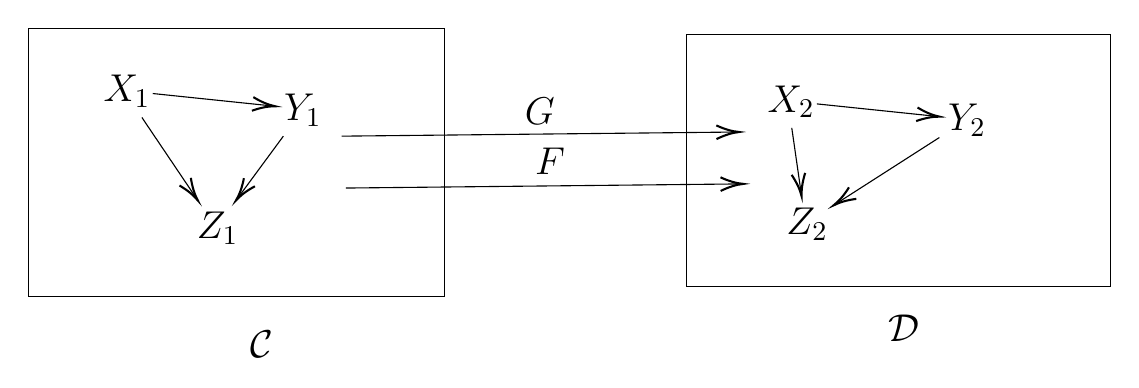
\begin{tikzpicture}[x=0.75pt,y=0.75pt,yscale=-1,xscale=1]
%uncomment if require: \path (0,300); %set diagram left start at 0, and has height of 300

%Shape: Rectangle [id:dp583091700239915] 
\draw   (66,78) -- (266.5,78) -- (266.5,207.07) -- (66,207.07) -- cycle ;
%Shape: Rectangle [id:dp2047555694997948] 
\draw   (383,81) -- (587.5,81) -- (587.5,202.33) -- (383,202.33) -- cycle ;
%Straight Lines [id:da9244423735196277] 
\draw    (219,155) -- (408.5,153.02) ;
\draw [shift={(410.5,153)}, rotate = 179.4] [color={rgb, 255:red, 0; green, 0; blue, 0 }  ][line width=0.75]    (10.93,-3.29) .. controls (6.95,-1.4) and (3.31,-0.3) .. (0,0) .. controls (3.31,0.3) and (6.95,1.4) .. (10.93,3.29)   ;
%Straight Lines [id:da5065283240152253] 
\draw    (217,130) -- (406.5,128.02) ;
\draw [shift={(408.5,128)}, rotate = 179.4] [color={rgb, 255:red, 0; green, 0; blue, 0 }  ][line width=0.75]    (10.93,-3.29) .. controls (6.95,-1.4) and (3.31,-0.3) .. (0,0) .. controls (3.31,0.3) and (6.95,1.4) .. (10.93,3.29)   ;

% Text Node
\draw (171.89,222.52) node [anchor=north west][inner sep=0.75pt]    {$\mathcal{C}$};
% Text Node
\draw (479.2,214.96) node [anchor=north west][inner sep=0.75pt]    {$\mathcal{D}$};
% Text Node
\draw (101,99.4) node [anchor=north west][inner sep=0.75pt]    {$X_{1}$};
% Text Node
\draw (188,108.4) node [anchor=north west][inner sep=0.75pt]    {$Y_{1}$};
% Text Node
\draw (146,165.4) node [anchor=north west][inner sep=0.75pt]    {$Z_{1}$};
% Text Node
\draw (421,104.4) node [anchor=north west][inner sep=0.75pt]    {$X_{2}$};
% Text Node
\draw (508,113.4) node [anchor=north west][inner sep=0.75pt]    {$Y_{2}$};
% Text Node
\draw (430,163.4) node [anchor=north west][inner sep=0.75pt]    {$Z_{2}$};
% Text Node
\draw (309,134.4) node [anchor=north west][inner sep=0.75pt]    {$F$};
% Text Node
\draw (304,110.4) node [anchor=north west][inner sep=0.75pt]    {$G$};
% Connection
\draw    (120.77,121) -- (146.62,159.34) ;
\draw [shift={(147.73,161)}, rotate = 236.01] [color={rgb, 255:red, 0; green, 0; blue, 0 }  ][line width=0.75]    (10.93,-3.29) .. controls (6.95,-1.4) and (3.31,-0.3) .. (0,0) .. controls (3.31,0.3) and (6.95,1.4) .. (10.93,3.29)   ;
% Connection
\draw    (126,109.46) -- (183.01,115.39) ;
\draw [shift={(185,115.6)}, rotate = 185.94] [color={rgb, 255:red, 0; green, 0; blue, 0 }  ][line width=0.75]    (10.93,-3.29) .. controls (6.95,-1.4) and (3.31,-0.3) .. (0,0) .. controls (3.31,0.3) and (6.95,1.4) .. (10.93,3.29)   ;
% Connection
\draw    (188.92,130) -- (167.27,159.39) ;
\draw [shift={(166.08,161)}, rotate = 306.38] [color={rgb, 255:red, 0; green, 0; blue, 0 }  ][line width=0.75]    (10.93,-3.29) .. controls (6.95,-1.4) and (3.31,-0.3) .. (0,0) .. controls (3.31,0.3) and (6.95,1.4) .. (10.93,3.29)   ;
% Connection
\draw    (433.87,126) -- (438.34,157.02) ;
\draw [shift={(438.63,159)}, rotate = 261.8] [color={rgb, 255:red, 0; green, 0; blue, 0 }  ][line width=0.75]    (10.93,-3.29) .. controls (6.95,-1.4) and (3.31,-0.3) .. (0,0) .. controls (3.31,0.3) and (6.95,1.4) .. (10.93,3.29)   ;
% Connection
\draw    (446,114.46) -- (503.01,120.39) ;
\draw [shift={(505,120.6)}, rotate = 185.94] [color={rgb, 255:red, 0; green, 0; blue, 0 }  ][line width=0.75]    (10.93,-3.29) .. controls (6.95,-1.4) and (3.31,-0.3) .. (0,0) .. controls (3.31,0.3) and (6.95,1.4) .. (10.93,3.29)   ;
% Connection
\draw    (505,130.65) -- (455.68,162.27) ;
\draw [shift={(454,163.35)}, rotate = 327.34] [color={rgb, 255:red, 0; green, 0; blue, 0 }  ][line width=0.75]    (10.93,-3.29) .. controls (6.95,-1.4) and (3.31,-0.3) .. (0,0) .. controls (3.31,0.3) and (6.95,1.4) .. (10.93,3.29)   ;

\end{tikzpicture}
    \end{center}
\end{definitionenv}
\begin{exampleenv}
    $P:\underline{\mathrm{CRing}}\rightarrow\underline{\mathrm{Set}}$.
    
    $\forall A\in \Obj(\mathbf{CRing})$,
    $$P(A)=\{(x,y,z)\in A^3\mid x^2+y^2=z^2\},$$
    $\forall f:A\rightarrow B$,
    $$ \begin{array}{rrcl}
        P(f):&P(A)&\rightarrow& P(B)\\
        &(x,y,z)&\mapsto&(f(x),f(y),f(z)).
    \end{array}
    $$
\end{exampleenv}
\begin{exampleenv}
    Let $\mathcal{C}$ be a category and $X\in\Obj\left(\mathcal{C}\right)$. We denote by $h_X:\mathcal{C}\rightarrow\underline{\mathrm{Set}}$, sending $Y\in \Obj(\mathcal{C})$ to $\mathcal{C}(X,Y)$.

    \quad If $f:Y\rightarrow Z$ is a morphism in $\mathcal{C}$,
    $$\begin{array}{rrcl}
        h_X(f):& \mathcal{C}(X,Y)&\rightarrow &\mathcal{C}(X,Z)\\
        & g&\mapsto&f\circ g\\
        \Id_{\mathcal{C}(X,Y)}=h_X(\Id_Y):&\mathcal{C}(X,Y)&\rightarrow & \mathcal{C}(X,Y)\\
        & g&\mapsto& \Id_Y\circ g = g
    \end{array}
    $$
    \begin{figure}[H]
        \centering


\tikzset{every picture/.style={line width=0.75pt}} %set default line width to 0.75pt        

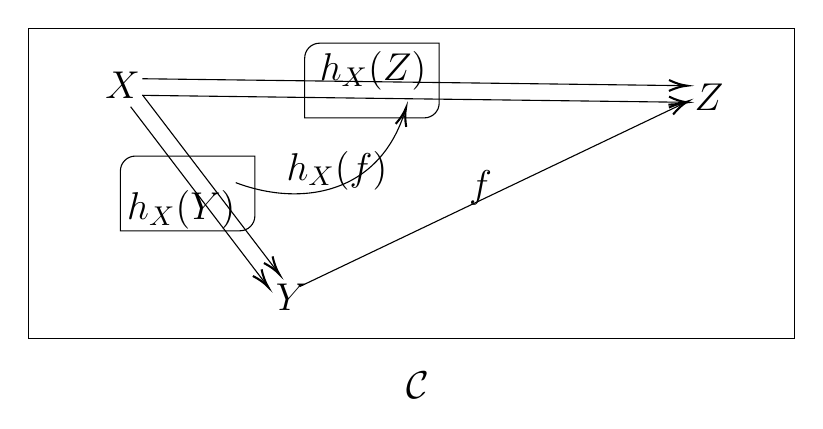
\begin{tikzpicture}[x=0.75pt,y=0.75pt,yscale=-1,xscale=1, scale = 0.8]
%uncomment if require: \path (0,300); %set diagram left start at 0, and has height of 300

%Shape: Rectangle [id:dp6898378251500559] 
\draw   (86,26) -- (547.5,26) -- (547.5,212.71) -- (86,212.71) -- cycle ;
%Rounded Diagonal Corner Rect [id:dp90110473299386] 
\draw   (141.5,112) .. controls (141.5,107.03) and (145.53,103) .. (150.5,103) -- (222.5,103) .. controls (222.5,103) and (222.5,103) .. (222.5,103) -- (222.5,139) .. controls (222.5,143.97) and (218.47,148) .. (213.5,148) -- (141.5,148) .. controls (141.5,148) and (141.5,148) .. (141.5,148) -- cycle ;
%Rounded Diagonal Corner Rect [id:dp20981670874217795] 
\draw   (252.5,44) .. controls (252.5,39.03) and (256.53,35) .. (261.5,35) -- (333.5,35) .. controls (333.5,35) and (333.5,35) .. (333.5,35) -- (333.5,71) .. controls (333.5,75.97) and (329.47,80) .. (324.5,80) -- (252.5,80) .. controls (252.5,80) and (252.5,80) .. (252.5,80) -- cycle ;
%Curve Lines [id:da18061312650610728] 
\draw    (211,119) .. controls (250.11,133.85) and (297.54,126.16) .. (313.04,75.55) ;
\draw [shift={(313.5,74)}, rotate = 106.09] [color={rgb, 255:red, 0; green, 0; blue, 0 }  ][line width=0.75]    (10.93,-3.29) .. controls (6.95,-1.4) and (3.31,-0.3) .. (0,0) .. controls (3.31,0.3) and (6.95,1.4) .. (10.93,3.29)   ;

% Text Node
\draw (312.19,231.45) node [anchor=north west][inner sep=0.75pt]    {$\mathcal{C}$};
% Text Node
\draw (130.81,50.69) node [anchor=north west][inner sep=0.75pt]    {$X$};
% Text Node
\draw (485.82,58.14) node [anchor=north west][inner sep=0.75pt]    {$Z$};
% Text Node
\draw (233.55,178.5) node [anchor=north west][inner sep=0.75pt]    {$Y$};
% Text Node
\draw (144,122.4) node [anchor=north west][inner sep=0.75pt]    {$h_{X}( Y)$};
% Text Node
\draw (350,110.4) node [anchor=north west][inner sep=0.75pt]    {$f$};
% Text Node
\draw (260,38.4) node [anchor=north west][inner sep=0.75pt]    {$h_{X}( Z)$};
% Text Node
\draw (240,98.4) node [anchor=north west][inner sep=0.75pt]    {$h_{X}( f)$};
% Connection
\draw    (154.81,66.16) -- (235.97,172.51) ;
\draw [shift={(237.18,174.1)}, rotate = 232.66] [color={rgb, 255:red, 0; green, 0; blue, 0 }  ][line width=0.75]    (10.93,-3.29) .. controls (6.95,-1.4) and (3.31,-0.3) .. (0,0) .. controls (3.31,0.3) and (6.95,1.4) .. (10.93,3.29)   ;
% Connection
\draw    (147.68,73.29) -- (229.33,180.31) ;
\draw [shift={(230.55,181.9)}, rotate = 232.66] [color={rgb, 255:red, 0; green, 0; blue, 0 }  ][line width=0.75]    (10.93,-3.29) .. controls (6.95,-1.4) and (3.31,-0.3) .. (0,0) .. controls (3.31,0.3) and (6.95,1.4) .. (10.93,3.29)   ;
% Connection
\draw    (154.81,56.42) -- (480.82,60.59) ;
\draw [shift={(482.82,60.62)}, rotate = 180.73] [color={rgb, 255:red, 0; green, 0; blue, 0 }  ][line width=0.75]    (10.93,-3.29) .. controls (6.95,-1.4) and (3.31,-0.3) .. (0,0) .. controls (3.31,0.3) and (6.95,1.4) .. (10.93,3.29)   ;
% Connection
\draw    (249.55,181.57) -- (481.01,71.13) ;
\draw [shift={(482.82,70.27)}, rotate = 154.49] [color={rgb, 255:red, 0; green, 0; blue, 0 }  ][line width=0.75]    (10.93,-3.29) .. controls (6.95,-1.4) and (3.31,-0.3) .. (0,0) .. controls (3.31,0.3) and (6.95,1.4) .. (10.93,3.29)   ;
% Connection
\draw    (154.81,66.42) -- (480.82,70.59) ;
\draw [shift={(482.82,70.62)}, rotate = 180.73] [color={rgb, 255:red, 0; green, 0; blue, 0 }  ][line width=0.75]    (10.93,-3.29) .. controls (6.95,-1.4) and (3.31,-0.3) .. (0,0) .. controls (3.31,0.3) and (6.95,1.4) .. (10.93,3.29)   ;

\end{tikzpicture}
    \end{figure}

$$\begin{array}{rrcl}
    h_X\left(\nu\circ\mu\right):&\mathcal{C}(X,Y) & \rightarrow &\mathcal{C}(X,W)\\
    & g &\rightarrow &\left(\nu\circ\mu\right)\circ g = \nu\circ \left(\mu\circ g\right)
\end{array}
$$
$$\mu\circ g = h_X(\mu)(g),$$

\begin{center}
\begin{tikzcd}
Y \arrow[r,  "\mu"] \arrow[dr,  swap,  "\nu\circ\mu"] &Z \arrow[d,  "\nu"] \\
& W
\end{tikzcd}
\end{center}
so,
$$\nu\circ\left(\mu\circ g\right) = h_X(\nu)\left(h_X(\mu)(g)\right),\ h_X(\nu\circ\mu) = h_X(\nu)\circ h_X(\mu).$$
\end{exampleenv}
\begin{exampleenv}
    Let $\mathcal{C}$ be a category. $\Id_\mathcal{C}$ that sends $X\in \Obj(C)$ to $X$ and $f:X\rightarrow Y$ to $f$. This is a functor.
\end{exampleenv}
\begin{exampleenv}
    Let $\mathcal{C}$, $\mathcal{D}$, $\mathcal{E}$ be categories, $F:\mathcal{C}\rightarrow\mathcal{D}$ and $G:\mathcal{D}\rightarrow\mathcal{E}$ be functors. We define a functor
    $$G\circ F:\mathcal{C}\rightarrow \mathcal{E}$$
    such that 
    $$\forall X\in \Obj(\mathcal{C}),\ \left(G\circ F\right)(X)=G(F(X)),$$
    $$\forall f:X\rightarrow Y,\ \left(G\circ F\right)(f) = G(F(f)).$$
\end{exampleenv}
\begin{definitionenv}
    Let $\mathcal{C}$ and $\mathcal{D}$ be categories, and $F:\mathcal{C}\rightarrow \mathcal{D}$ and $G:\mathcal{C}\rightarrow\mathcal{D}$ be functors. We call natural transformation (morphism of function) from $F$ to $G$ any family
    $$\varphi=\left(\varphi_X\right)_{X\in \Obj(\mathcal{C})}$$
    where $\varphi_X:F(X)\rightarrow G(X)$ is a morphism (in $\mathcal{D}$) such that for any morphism $f:X\rightarrow Y$ in $\mathcal{C}$, the following diagram is commutative:
    \begin{center}
    \begin{tikzcd}
F(X) \arrow[r,  "F(f)"] \arrow[d,  swap,  "\varphi_{X}"] &\displaystyle F(Y) \arrow[d,  "\varphi_Y"] \\
G(X) \arrow[r,"G(f)"]& G(Y)
\end{tikzcd}
\end{center}
$$G(f)\circ \varphi_X=\varphi_Y\circ F(f).$$
\begin{figure}[H]
    \centering


\tikzset{every picture/.style={line width=0.75pt}} %set default line width to 0.75pt        

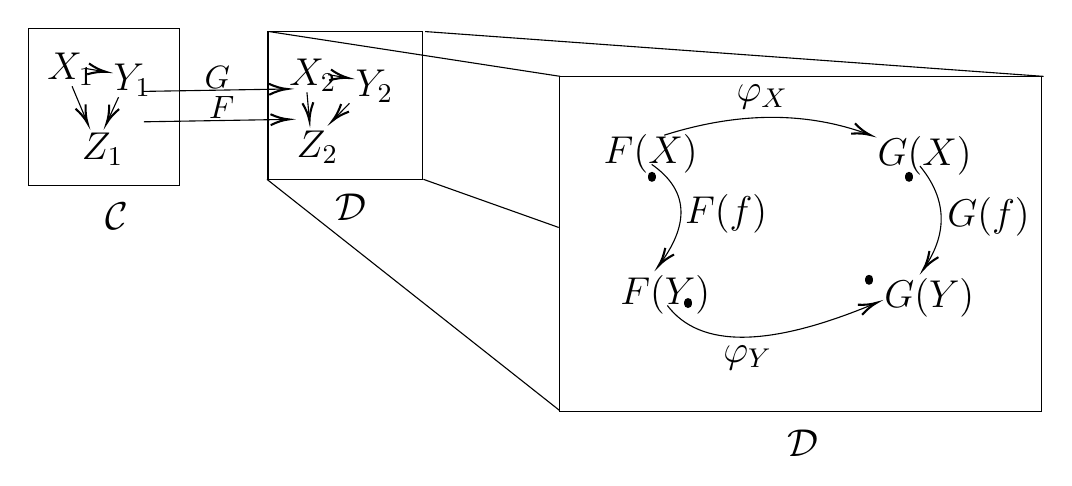
\begin{tikzpicture}[x=0.75pt,y=0.75pt,yscale=-1,xscale=1, scale = 0.8]
%uncomment if require: \path (0,300); %set diagram left start at 0, and has height of 300

%Shape: Rectangle [id:dp7089110550670655] 
\draw   (16,19) -- (107.31,19) -- (107.31,113.48) -- (16,113.48) -- cycle ;
%Shape: Rectangle [id:dp6149851284848306] 
\draw   (160.37,21.2) -- (253.5,21.2) -- (253.5,110.01) -- (160.37,110.01) -- cycle ;
%Straight Lines [id:da9596541637490664] 
\draw    (85.68,75.36) -- (170.89,73.93) ;
\draw [shift={(172.89,73.9)}, rotate = 179.04] [color={rgb, 255:red, 0; green, 0; blue, 0 }  ][line width=0.75]    (10.93,-3.29) .. controls (6.95,-1.4) and (3.31,-0.3) .. (0,0) .. controls (3.31,0.3) and (6.95,1.4) .. (10.93,3.29)   ;
%Straight Lines [id:da2100847392454801] 
\draw    (84.77,57.06) -- (169.98,55.63) ;
\draw [shift={(171.98,55.6)}, rotate = 179.04] [color={rgb, 255:red, 0; green, 0; blue, 0 }  ][line width=0.75]    (10.93,-3.29) .. controls (6.95,-1.4) and (3.31,-0.3) .. (0,0) .. controls (3.31,0.3) and (6.95,1.4) .. (10.93,3.29)   ;
%Shape: Rectangle [id:dp1302044156137787] 
\draw   (336,48) -- (626.5,48) -- (626.5,250) -- (336,250) -- cycle ;
%Straight Lines [id:da036506408298424] 
\draw    (159.78,110.02) -- (335.78,249.02) ;
%Straight Lines [id:da8328603435353752] 
\draw    (255,21) -- (627.5,48) ;
%Shape: Free Drawing [id:dp9920703584396833] 
\draw  [line width=3] [line join = round][line cap = round] (391.5,108) .. controls (391.5,108.33) and (391.5,108.67) .. (391.5,109) ;
%Shape: Free Drawing [id:dp7832409228988187] 
\draw  [line width=3] [line join = round][line cap = round] (546.5,108) .. controls (546.5,108.33) and (546.5,108.67) .. (546.5,109) ;
%Shape: Free Drawing [id:dp8584801540259973] 
\draw  [line width=3] [line join = round][line cap = round] (413.5,184) .. controls (413.5,184.33) and (413.5,184.67) .. (413.5,185) ;
%Shape: Free Drawing [id:dp8934882364262572] 
\draw  [line width=3] [line join = round][line cap = round] (522.5,170) .. controls (522.5,170.33) and (522.5,170.67) .. (522.5,171) ;
%Straight Lines [id:da8036087358907691] 
\draw    (254,110) -- (335.5,139) ;
%Straight Lines [id:da9261767614907577] 
\draw    (161,21) -- (336.5,48) ;

% Text Node
\draw (60.68,122.75) node [anchor=north west][inner sep=0.75pt]    {$\mathcal{C}$};
% Text Node
\draw (199.55,117.21) node [anchor=north west][inner sep=0.75pt]    {$\mathcal{D}$};
% Text Node
\draw (25.95,32.36) node [anchor=north west][inner sep=0.75pt]    {$X_{1}$};
% Text Node
\draw (65.84,38.95) node [anchor=north west][inner sep=0.75pt]    {$Y_{1}$};
% Text Node
\draw (46.72,80.67) node [anchor=north west][inner sep=0.75pt]    {$Z_{1}$};
% Text Node
\draw (171.68,36.02) node [anchor=north west][inner sep=0.75pt]    {$X_{2}$};
% Text Node
\draw (211.58,42.61) node [anchor=north west][inner sep=0.75pt]    {$Y_{2}$};
% Text Node
\draw (176.05,79.2) node [anchor=north west][inner sep=0.75pt]    {$Z_{2}$};
% Text Node
\draw (123.4,58.25) node [anchor=north west][inner sep=0.75pt]    {\footnotesize$F$};
% Text Node
\draw (120.58,40.68) node [anchor=north west][inner sep=0.75pt]    {\footnotesize$G$};
% Text Node
\draw (471.55,259.21) node [anchor=north west][inner sep=0.75pt]    {$\mathcal{D}$};
% Text Node
\draw (361,81.4) node [anchor=north west][inner sep=0.75pt]    {$F( X)$};
% Text Node
\draw (526,82.4) node [anchor=north west][inner sep=0.75pt]    {$G( X)$};
% Text Node
\draw (371,166.4) node [anchor=north west][inner sep=0.75pt]    {$F( Y)$};
% Text Node
\draw (530,168.4) node [anchor=north west][inner sep=0.75pt]    {$G( Y)$};
% Text Node
\draw (441,51.4) node [anchor=north west][inner sep=0.75pt]    {$\varphi _{X}$};
% Text Node
\draw (433,208.4) node [anchor=north west][inner sep=0.75pt]    {$\varphi _{Y}$};
% Text Node
\draw (410,117.4) node [anchor=north west][inner sep=0.75pt]    {$F( f)$};
% Text Node
\draw (568,119.4) node [anchor=north west][inner sep=0.75pt]    {$G( f)$};
% Connection
\draw    (42.4,53.96) -- (50.99,74.42) ;
\draw [shift={(51.76,76.27)}, rotate = 247.24] [color={rgb, 255:red, 0; green, 0; blue, 0 }  ][line width=0.75]    (10.93,-3.29) .. controls (6.95,-1.4) and (3.31,-0.3) .. (0,0) .. controls (3.31,0.3) and (6.95,1.4) .. (10.93,3.29)   ;
% Connection
\draw    (50.95,43.3) -- (60.87,44.96) ;
\draw [shift={(62.84,45.29)}, rotate = 189.49] [color={rgb, 255:red, 0; green, 0; blue, 0 }  ][line width=0.75]    (10.93,-3.29) .. controls (6.95,-1.4) and (3.31,-0.3) .. (0,0) .. controls (3.31,0.3) and (6.95,1.4) .. (10.93,3.29)   ;
% Connection
\draw    (70.38,60.55) -- (64.01,74.45) ;
\draw [shift={(63.18,76.27)}, rotate = 294.63] [color={rgb, 255:red, 0; green, 0; blue, 0 }  ][line width=0.75]    (10.93,-3.29) .. controls (6.95,-1.4) and (3.31,-0.3) .. (0,0) .. controls (3.31,0.3) and (6.95,1.4) .. (10.93,3.29)   ;
% Connection
\draw    (183.85,57.62) -- (185.21,72.81) ;
\draw [shift={(185.39,74.8)}, rotate = 264.88] [color={rgb, 255:red, 0; green, 0; blue, 0 }  ][line width=0.75]    (10.93,-3.29) .. controls (6.95,-1.4) and (3.31,-0.3) .. (0,0) .. controls (3.31,0.3) and (6.95,1.4) .. (10.93,3.29)   ;
% Connection
\draw    (196.68,46.96) -- (206.6,48.62) ;
\draw [shift={(208.58,48.95)}, rotate = 189.49] [color={rgb, 255:red, 0; green, 0; blue, 0 }  ][line width=0.75]    (10.93,-3.29) .. controls (6.95,-1.4) and (3.31,-0.3) .. (0,0) .. controls (3.31,0.3) and (6.95,1.4) .. (10.93,3.29)   ;
% Connection
\draw    (209.46,64.21) -- (200.56,73.37) ;
\draw [shift={(199.17,74.8)}, rotate = 314.15] [color={rgb, 255:red, 0; green, 0; blue, 0 }  ][line width=0.75]    (10.93,-3.29) .. controls (6.95,-1.4) and (3.31,-0.3) .. (0,0) .. controls (3.31,0.3) and (6.95,1.4) .. (10.93,3.29)   ;
% Connection
\draw    (399,83.43) .. controls (443.33,69.35) and (484.09,69.09) .. (521.3,82.65) ;
\draw [shift={(523,83.28)}, rotate = 200.64] [color={rgb, 255:red, 0; green, 0; blue, 0 }  ][line width=0.75]    (10.93,-3.29) .. controls (6.95,-1.4) and (3.31,-0.3) .. (0,0) .. controls (3.31,0.3) and (6.95,1.4) .. (10.93,3.29)   ;
% Connection
\draw    (400.92,186) .. controls (420.54,211.87) and (462.25,211.44) .. (526.04,184.73) ;
\draw [shift={(527,184.32)}, rotate = 157.14] [color={rgb, 255:red, 0; green, 0; blue, 0 }  ][line width=0.75]    (10.93,-3.29) .. controls (6.95,-1.4) and (3.31,-0.3) .. (0,0) .. controls (3.31,0.3) and (6.95,1.4) .. (10.93,3.29)   ;
% Connection
\draw    (391.47,101) .. controls (413.05,116.02) and (414.84,135.86) .. (396.82,160.49) ;
\draw [shift={(395.69,162)}, rotate = 307.18] [color={rgb, 255:red, 0; green, 0; blue, 0 }  ][line width=0.75]    (10.93,-3.29) .. controls (6.95,-1.4) and (3.31,-0.3) .. (0,0) .. controls (3.31,0.3) and (6.95,1.4) .. (10.93,3.29)   ;
% Connection
\draw    (553.03,102) .. controls (568.91,121.33) and (570.01,141.47) .. (556.33,162.39) ;
\draw [shift={(555.25,164)}, rotate = 304.57] [color={rgb, 255:red, 0; green, 0; blue, 0 }  ][line width=0.75]    (10.93,-3.29) .. controls (6.95,-1.4) and (3.31,-0.3) .. (0,0) .. controls (3.31,0.3) and (6.95,1.4) .. (10.93,3.29)   ;

\end{tikzpicture}
\end{figure}
\end{definitionenv}
\begin{exampleenv}
    Let $\Id_F$ be the family $\left(\Id_{F(X)}\right)_{X\in \Obj(\mathcal{C})}$. This is a morphism of functors from $F$ to $F$, called the identity morphism.
    \begin{center}
    \begin{tikzcd}
F(X) \arrow[r,  "F(f)"] \arrow[d,  swap,  "\Id_{F(X)}"] &\displaystyle F(Y) \arrow[d,  "\Id_{F(Y)}"] \\
F(X) \arrow[r,"F(f)"]& F(Y)
\end{tikzcd}
\end{center}
$$F(f)\circ \Id_{F(X)} = F(f) =\Id_{F(Y)}\circ F(f).$$
\end{exampleenv}
\begin{exampleenv}
    Let $F$, $G$ and $H$ be functors from $\mathcal{C}$ to $\mathcal{D}$, $\varphi: F\rightarrow G$, $\psi:G\rightarrow H$ be natural transformations. We define
    $$\psi\circ \varphi: F\rightarrow H$$
    as the family 
    $$ \left(\psi_X\circ\varphi_X\right)_{X\in \Obj(\mathcal{C})},\ F(X)\overset{\varphi_X}{\longrightarrow}G(X)\overset{\psi_X}{\longrightarrow}H(X).$$
    It is called the composite of $\psi$ and $\varphi$.
\end{exampleenv}
\begin{remark}
    Let $\mathcal{C}$ and $\mathcal{D}$ be categories. Let $\underline{\mathrm{Fun}}(\mathcal{C},\mathcal{D})$ be the data that is composite of
    \begin{itemize}
        \item The set of all functors from $\mathcal{C}$ to $\mathcal{D}$
        \item Natural transformations.
    \end{itemize}
    Then $\underline{\mathrm{Fun}}(\mathcal{C},\mathcal{D})$ forms a category (in some suitable universe). It is called the category of functors from $\mathcal{C}$ to $\mathcal{D}$. If $F$ and $G$ are two functors from $\mathcal{C}$ to $\mathcal{D}$ such that there exists an isomorphism from $F$ to $G$ in $\underline{\mathrm{Fun}}(\mathcal{C},\mathcal{D})$. We say that $F$ and $G$ are isomorphic.
\end{remark}
\begin{propositionenv}
    Let $\mathcal{U}$ be a universe, $\mathcal{C}$ be a $\mathcal{U}$-small category, and $\mathcal{D}$ be a $\mathcal{U}$-category. For any functors $F$ and $G$ from $\mathcal{C}$ to $\mathcal{D}$, the set $\mathrm{Nat}(F,G)$ of natural transformation from $F$ to $G$ belongs to $\mathcal{U}$.
\end{propositionenv}
\begin{proofenv}
    $\mathrm{Nat}(F,G)$ is a subset of $\dis \prod_{X\in \Obj(\mathcal{C})}\mathcal{D}(F(X),G(X))\in \mathcal{U}$.
\end{proofenv}
\begin{notationenv}
    If $\mathcal{C}$ is a category, then $\underline{\mathrm{Fun}}(\mathcal{C},\underline{\mathrm{Set}})$ is denoted by $\hat{\mathcal{C}}$.
\end{notationenv}
\newpage
\section{Yoneda Lemma}
\begin{theoremenv}
    Let $\mathcal{C}$ be a category, $F:\mathcal{C}\rightarrow \underline{\mathrm{Set}}$ be a functor and $X\in \Obj(\mathcal{C})$. Then
    $$\begin{array}{rrcl}
        \beta:&\mathrm{Nat}(h_X,F)&\rightarrow& F(X)\\
        & \psi&\mapsto&\psi_X(\Id_X)\footnote{$\psi_X:h_X(X)=\mathcal{C}(X,X)\rightarrow F(X)$.}
    \end{array}$$
    is a bijection.
    \begin{figure}[H]
    \centering


\tikzset{every picture/.style={line width=0.75pt}} %set default line width to 0.75pt        

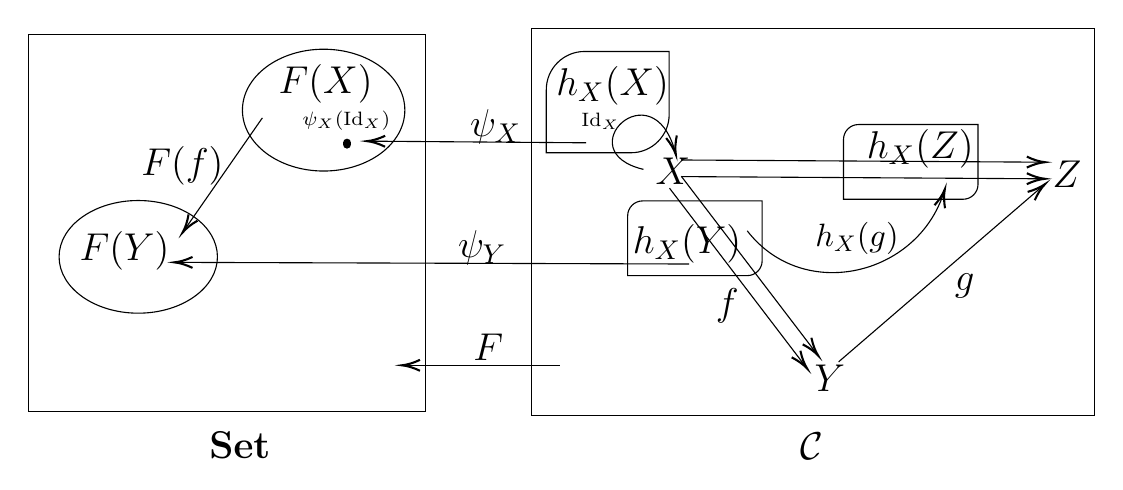
\begin{tikzpicture}[x=0.75pt,y=0.75pt,yscale=-1,xscale=1, scale =0.8]
%uncomment if require: \path (0,300); %set diagram left start at 0, and has height of 300

%Shape: Rectangle [id:dp29104558201405406] 
\draw   (314.5,30) -- (653.5,30) -- (653.5,263) -- (314.5,263) -- cycle ;
%Rounded Diagonal Corner Rect [id:dp44417459474777166] 
\draw   (372.5,143) .. controls (372.5,138.03) and (376.53,134) .. (381.5,134) -- (453.5,134) .. controls (453.5,134) and (453.5,134) .. (453.5,134) -- (453.5,170) .. controls (453.5,174.97) and (449.47,179) .. (444.5,179) -- (372.5,179) .. controls (372.5,179) and (372.5,179) .. (372.5,179) -- cycle ;
%Rounded Diagonal Corner Rect [id:dp5510703091888516] 
\draw   (502.5,97) .. controls (502.5,92.03) and (506.53,88) .. (511.5,88) -- (583.5,88) .. controls (583.5,88) and (583.5,88) .. (583.5,88) -- (583.5,124) .. controls (583.5,128.97) and (579.47,133) .. (574.5,133) -- (502.5,133) .. controls (502.5,133) and (502.5,133) .. (502.5,133) -- cycle ;
%Curve Lines [id:da6732018462293708] 
\draw    (444.5,152) .. controls (478.16,195.56) and (547.1,179.33) .. (563.03,128.55) ;
\draw [shift={(563.5,127)}, rotate = 106.09] [color={rgb, 255:red, 0; green, 0; blue, 0 }  ][line width=0.75]    (10.93,-3.29) .. controls (6.95,-1.4) and (3.31,-0.3) .. (0,0) .. controls (3.31,0.3) and (6.95,1.4) .. (10.93,3.29)   ;
%Shape: Rectangle [id:dp49619736846033] 
\draw   (11.5,34) -- (250.5,34) -- (250.5,261) -- (11.5,261) -- cycle ;
%Shape: Ellipse [id:dp5211352656838969] 
\draw   (140.5,79.32) .. controls (140.5,59.06) and (162.4,42.64) .. (189.4,42.64) .. controls (216.41,42.64) and (238.31,59.06) .. (238.31,79.32) .. controls (238.31,99.58) and (216.41,116) .. (189.4,116) .. controls (162.4,116) and (140.5,99.58) .. (140.5,79.32) -- cycle ;
%Straight Lines [id:da796610559906879] 
\draw    (331.5,233) -- (238.5,233) ;
\draw [shift={(236.5,233)}, rotate = 360] [color={rgb, 255:red, 0; green, 0; blue, 0 }  ][line width=0.75]    (10.93,-3.29) .. controls (6.95,-1.4) and (3.31,-0.3) .. (0,0) .. controls (3.31,0.3) and (6.95,1.4) .. (10.93,3.29)   ;
%Shape: Ellipse [id:dp4066346829093145] 
\draw   (30.08,167.69) .. controls (30.08,148.95) and (51.43,133.76) .. (77.76,133.76) .. controls (104.1,133.76) and (125.45,148.95) .. (125.45,167.69) .. controls (125.45,186.42) and (104.1,201.61) .. (77.76,201.61) .. controls (51.43,201.61) and (30.08,186.42) .. (30.08,167.69) -- cycle ;
%Rounded Diagonal Corner Rect [id:dp9719492308142043] 
\draw   (323.5,67.04) .. controls (323.5,54.32) and (333.82,44) .. (346.54,44) -- (397.5,44) .. controls (397.5,44) and (397.5,44) .. (397.5,44) -- (397.5,81.96) .. controls (397.5,94.68) and (387.18,105) .. (374.46,105) -- (323.5,105) .. controls (323.5,105) and (323.5,105) .. (323.5,105) -- cycle ;
%Curve Lines [id:da2752984146564955] 
\draw    (382,115) .. controls (335.97,104.11) and (387.45,54.02) .. (401.1,104.44) ;
\draw [shift={(401.5,106)}, rotate = 256.22] [color={rgb, 255:red, 0; green, 0; blue, 0 }  ][line width=0.75]    (10.93,-3.29) .. controls (6.95,-1.4) and (3.31,-0.3) .. (0,0) .. controls (3.31,0.3) and (6.95,1.4) .. (10.93,3.29)   ;
%Straight Lines [id:da19731840968168723] 
\draw    (347.5,99) -- (217.5,98.02) ;
\draw [shift={(215.5,98)}, rotate = 0.43] [color={rgb, 255:red, 0; green, 0; blue, 0 }  ][line width=0.75]    (10.93,-3.29) .. controls (6.95,-1.4) and (3.31,-0.3) .. (0,0) .. controls (3.31,0.3) and (6.95,1.4) .. (10.93,3.29)   ;
%Shape: Free Drawing [id:dp2493761350192819] 
\draw  [line width=3] [line join = round][line cap = round] (203.5,99) .. controls (203.5,99.33) and (203.5,99.67) .. (203.5,100) ;
%Straight Lines [id:da5093037449359683] 
\draw    (409.5,172) -- (101.5,171.01) ;
\draw [shift={(99.5,171)}, rotate = 0.18] [color={rgb, 255:red, 0; green, 0; blue, 0 }  ][line width=0.75]    (10.93,-3.29) .. controls (6.95,-1.4) and (3.31,-0.3) .. (0,0) .. controls (3.31,0.3) and (6.95,1.4) .. (10.93,3.29)   ;
%Straight Lines [id:da8188395842578471] 
\draw    (152.5,84) -- (105.64,151.36) ;
\draw [shift={(104.5,153)}, rotate = 304.82] [color={rgb, 255:red, 0; green, 0; blue, 0 }  ][line width=0.75]    (10.93,-3.29) .. controls (6.95,-1.4) and (3.31,-0.3) .. (0,0) .. controls (3.31,0.3) and (6.95,1.4) .. (10.93,3.29)   ;

% Text Node
\draw (475.19,272.45) node [anchor=north west][inner sep=0.75pt]    {$\mathcal{C}$};
% Text Node
\draw (387.81,106.69) node [anchor=north west][inner sep=0.75pt]    {$X$};
% Text Node
\draw (626.82,108.14) node [anchor=north west][inner sep=0.75pt]    {$Z$};
% Text Node
\draw (483.55,231.5) node [anchor=north west][inner sep=0.75pt]    {$Y$};
% Text Node
\draw (374,146.4) node [anchor=north west][inner sep=0.75pt]    {$h_{X}( Y)$};
% Text Node
\draw (568,176.4) node [anchor=north west][inner sep=0.75pt]    {$g$};
% Text Node
\draw (515,89.4) node [anchor=north west][inner sep=0.75pt]    {$h_{X}( Z)$};
% Text Node
\draw (484,145.4) node [anchor=north west][inner sep=0.75pt]    {\footnotesize$h_{X}( g)$};
% Text Node
\draw (119,271.4) node [anchor=north west][inner sep=0.75pt]    {$\mathbf{Set}$};
% Text Node
\draw (278,212.4) node [anchor=north west][inner sep=0.75pt]    {$F$};
% Text Node
\draw (160.74,50.52) node [anchor=north west][inner sep=0.75pt]    {$F( X)$};
% Text Node
\draw (40.85,150.65) node [anchor=north west][inner sep=0.75pt]    {$F( Y)$};
% Text Node
\draw (328,51.4) node [anchor=north west][inner sep=0.75pt]    {$h_{X}( X)$};
% Text Node
\draw (276,77.4) node [anchor=north west][inner sep=0.75pt]    {$\psi _{X}$};
% Text Node
\draw (343,79.4) node [anchor=north west][inner sep=0.75pt]    {\tiny$\mathrm{Id}_{X}$};
% Text Node
\draw (175,78.4) node [anchor=north west][inner sep=0.75pt]    {\tiny$\psi _{X}(\mathrm{Id}_{X})$};
% Text Node
\draw (268.77,150.4) node [anchor=north west][inner sep=0.75pt]    {$\psi _{Y}$};
% Text Node
\draw (424,185.4) node [anchor=north west][inner sep=0.75pt]    {$f$};
% Text Node
\draw (78,99.4) node [anchor=north west][inner sep=0.75pt]    {$F( f)$};
% Connection
\draw    (404.81,119.16) -- (485.97,225.51) ;
\draw [shift={(487.18,227.1)}, rotate = 232.66] [color={rgb, 255:red, 0; green, 0; blue, 0 }  ][line width=0.75]    (10.93,-3.29) .. controls (6.95,-1.4) and (3.31,-0.3) .. (0,0) .. controls (3.31,0.3) and (6.95,1.4) .. (10.93,3.29)   ;
% Connection
\draw    (397.68,126.29) -- (479.33,233.31) ;
\draw [shift={(480.55,234.9)}, rotate = 232.66] [color={rgb, 255:red, 0; green, 0; blue, 0 }  ][line width=0.75]    (10.93,-3.29) .. controls (6.95,-1.4) and (3.31,-0.3) .. (0,0) .. controls (3.31,0.3) and (6.95,1.4) .. (10.93,3.29)   ;
% Connection
\draw    (404.81,109.35) -- (621.82,110.67) ;
\draw [shift={(623.82,110.68)}, rotate = 180.35] [color={rgb, 255:red, 0; green, 0; blue, 0 }  ][line width=0.75]    (10.93,-3.29) .. controls (6.95,-1.4) and (3.31,-0.3) .. (0,0) .. controls (3.31,0.3) and (6.95,1.4) .. (10.93,3.29)   ;
% Connection
\draw    (499.55,230.92) -- (622.3,125.22) ;
\draw [shift={(623.82,123.92)}, rotate = 139.27] [color={rgb, 255:red, 0; green, 0; blue, 0 }  ][line width=0.75]    (10.93,-3.29) .. controls (6.95,-1.4) and (3.31,-0.3) .. (0,0) .. controls (3.31,0.3) and (6.95,1.4) .. (10.93,3.29)   ;
% Connection
\draw    (404.81,119.35) -- (621.82,120.67) ;
\draw [shift={(623.82,120.68)}, rotate = 180.35] [color={rgb, 255:red, 0; green, 0; blue, 0 }  ][line width=0.75]    (10.93,-3.29) .. controls (6.95,-1.4) and (3.31,-0.3) .. (0,0) .. controls (3.31,0.3) and (6.95,1.4) .. (10.93,3.29)   ;

\end{tikzpicture}
    \end{figure}
\end{theoremenv}
\begin{proofenv}
    We construct a mapping
    $$\begin{array}{rrcl}
        \alpha:&F(X)&\rightarrow&\mathrm{Nat}(h_X,F)\\
        &x&\mapsto&\alpha(x)=(\alpha(x)_Y)_{Y\in \Obj(\mathcal{C})}
    \end{array}
    $$
    \begin{figure}[H]
    \centering
\tikzset{every picture/.style={line width=0.75pt}} %set default line width to 0.75pt        

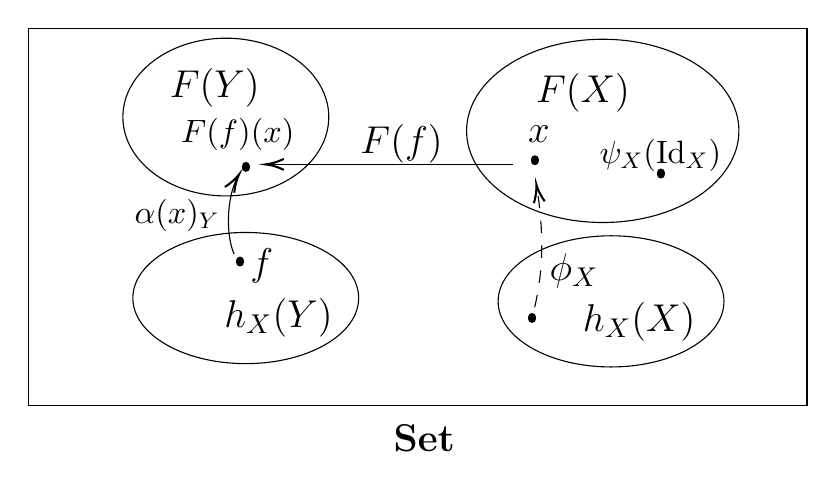
\begin{tikzpicture}[x=0.75pt,y=0.75pt,yscale=-1,xscale=1, scale = 0.8]
%uncomment if require: \path (0,300); %set diagram left start at 0, and has height of 300

%Shape: Rectangle [id:dp19892027739488838] 
\draw   (94.5,26) -- (563.5,26) -- (563.5,253) -- (94.5,253) -- cycle ;
%Shape: Ellipse [id:dp35634985592370083] 
\draw   (358.5,87.82) .. controls (358.5,57.34) and (395.21,32.64) .. (440.5,32.64) .. controls (485.79,32.64) and (522.5,57.34) .. (522.5,87.82) .. controls (522.5,118.29) and (485.79,143) .. (440.5,143) .. controls (395.21,143) and (358.5,118.29) .. (358.5,87.82) -- cycle ;
%Shape: Ellipse [id:dp7145581050737746] 
\draw   (151.5,79.5) .. controls (151.5,53.27) and (179.26,32) .. (213.5,32) .. controls (247.74,32) and (275.5,53.27) .. (275.5,79.5) .. controls (275.5,105.73) and (247.74,127) .. (213.5,127) .. controls (179.26,127) and (151.5,105.73) .. (151.5,79.5) -- cycle ;
%Shape: Free Drawing [id:dp5680895793130827] 
\draw  [line width=3] [line join = round][line cap = round] (475.5,113) .. controls (475.5,113.33) and (475.5,113.67) .. (475.5,114) ;
%Straight Lines [id:da4515185175819256] 
\draw    (386.5,108) -- (239.5,108) ;
\draw [shift={(237.5,108)}, rotate = 360] [color={rgb, 255:red, 0; green, 0; blue, 0 }  ][line width=0.75]    (10.93,-3.29) .. controls (6.95,-1.4) and (3.31,-0.3) .. (0,0) .. controls (3.31,0.3) and (6.95,1.4) .. (10.93,3.29)   ;
%Shape: Free Drawing [id:dp8664607428198391] 
\draw  [line width=3] [line join = round][line cap = round] (399.5,105) .. controls (399.5,105.33) and (399.5,105.67) .. (399.5,106) ;
%Shape: Free Drawing [id:dp8705631504135898] 
\draw  [line width=3] [line join = round][line cap = round] (225.5,109) .. controls (225.5,109.33) and (225.5,109.67) .. (225.5,110) ;
%Curve Lines [id:da06385969038265649] 
\draw  [dash pattern={on 4.5pt off 4.5pt}]  (399.5,194) .. controls (405.35,169.62) and (404.55,145.25) .. (400.79,121.8) ;
\draw [shift={(400.5,120)}, rotate = 80.54] [color={rgb, 255:red, 0; green, 0; blue, 0 }  ][line width=0.75]    (10.93,-3.29) .. controls (6.95,-1.4) and (3.31,-0.3) .. (0,0) .. controls (3.31,0.3) and (6.95,1.4) .. (10.93,3.29)   ;
%Shape: Ellipse [id:dp6467487281921943] 
\draw   (377.5,190.5) .. controls (377.5,168.68) and (407.94,151) .. (445.5,151) .. controls (483.06,151) and (513.5,168.68) .. (513.5,190.5) .. controls (513.5,212.32) and (483.06,230) .. (445.5,230) .. controls (407.94,230) and (377.5,212.32) .. (377.5,190.5) -- cycle ;
%Shape: Ellipse [id:dp4928430640278725] 
\draw   (157.5,188.5) .. controls (157.5,166.68) and (187.94,149) .. (225.5,149) .. controls (263.06,149) and (293.5,166.68) .. (293.5,188.5) .. controls (293.5,210.32) and (263.06,228) .. (225.5,228) .. controls (187.94,228) and (157.5,210.32) .. (157.5,188.5) -- cycle ;
%Shape: Free Drawing [id:dp819965093523772] 
\draw  [line width=3] [line join = round][line cap = round] (222.09,166) .. controls (222.09,166.33) and (222.09,166.67) .. (222.09,167) ;
%Curve Lines [id:da9112028098270881] 
\draw    (218.5,162) .. controls (213.7,151.44) and (213.51,128.9) .. (220.58,115.61) ;
\draw [shift={(221.5,114)}, rotate = 121.61] [color={rgb, 255:red, 0; green, 0; blue, 0 }  ][line width=0.75]    (10.93,-3.29) .. controls (6.95,-1.4) and (3.31,-0.3) .. (0,0) .. controls (3.31,0.3) and (6.95,1.4) .. (10.93,3.29)   ;
%Shape: Free Drawing [id:dp6961614065798236] 
\draw  [line width=3] [line join = round][line cap = round] (398.09,200) .. controls (398.09,200.33) and (398.09,200.67) .. (398.09,201) ;

% Text Node
\draw (313,263.4) node [anchor=north west][inner sep=0.75pt]    {$\mathbf{Set}$};
% Text Node
\draw (398.74,51.52) node [anchor=north west][inner sep=0.75pt]    {$F( X)$};
% Text Node
\draw (178.24,48.76) node [anchor=north west][inner sep=0.75pt]    {$F( Y)$};
% Text Node
\draw (437,91.4) node [anchor=north west][inner sep=0.75pt]    {\footnotesize$\psi _{X}(\mathrm{Id}_{X})$};
% Text Node
\draw (293,82.4) node [anchor=north west][inner sep=0.75pt]    {$F( f)$};
% Text Node
\draw (394,83.4) node [anchor=north west][inner sep=0.75pt]    {$x$};
% Text Node
\draw (185,78.4) node [anchor=north west][inner sep=0.75pt]    {\footnotesize$F( f)( x)$};
% Text Node
\draw (407,160.4) node [anchor=north west][inner sep=0.75pt]    {$\phi _{X}$};
% Text Node
\draw (427,189.4) node [anchor=north west][inner sep=0.75pt]    {$h_{X}( X)$};
% Text Node
\draw (211,187.4) node [anchor=north west][inner sep=0.75pt]    {$h_{X}( Y)$};
% Text Node
\draw (226.75,157.4) node [anchor=north west][inner sep=0.75pt]    {$f$};
% Text Node
\draw (157,127.4) node [anchor=north west][inner sep=0.75pt]    {\footnotesize$\alpha ( x)_{Y}$};


\end{tikzpicture}
\end{figure}
    where $\alpha(x)_{Y}:h_X(Y)=\mathcal{C}(X,Y)\rightarrow F(Y)$, $f\mapsto F(f)(x)$. We need to check that $\alpha(x)$ is a natural transformation.
    Namely, for any $ \mu:A\rightarrow B$ in $\mathcal{C}$, we have a commutative diagram
    \begin{center}
    \begin{tikzcd}
\mathcal{C}(X,A) \arrow[d, swap, "\alpha(x)_A"]  \arrow[r, "h_X(\mu)"]& \mathcal{C}(X,B) \arrow[d,  "\alpha(x)_B"] \\
F(A) \arrow[r,"F(\mu)"]& F(B)  
\end{tikzcd}
\end{center}
In fact, 
$\forall f\in \mathcal{C}(X,A)$, $$\alpha(x)_B(h_X(\mu)(f))=\alpha(x)_B(\mu\circ f)=F(\mu\circ f)(x),$$
$$F(\mu)\left(\alpha(x)_A(f)\right) = F(\mu)\left(F(f)(x)\right)=F(\mu\circ f)(x).$$
We then check that $\alpha$ and $\beta$ are inverse of each other.
\begin{itemize}
    \item Let $\psi:h_X\rightarrow F$ be a natural transformation and $x=\psi_X(\Id_X)$. For any $f:X\rightarrow Y$ in $\mathcal{C}$,
    $$\alpha(x)_{Y}(f) = F(f)(x) = F(f)\left(\psi_X(\Id_X)\right)=\psi_Y\left(h_X(f)(\Id_X)\right)=\psi_Y(f).$$
    So, $\alpha(x)=\psi$.
    \item For any $x\in F(x)$,
    $$ \beta\left(\alpha(x)\right)=\alpha(x)_X\left(\Id_X\right)= F(\Id_X)(x) = \Id_{F(X)}(x)=x.$$
\end{itemize}
    \begin{center}
    \begin{tikzcd}
h_X(X) \arrow[r,  "F(f)"] \arrow[d,  swap,  "\psi_X"] &\displaystyle F(Y) \arrow[d,  "\psi_Y"] \\
F(X) \arrow[r,"F(f)"]& F(Y)
\end{tikzcd}
\end{center}
\end{proofenv}
\begin{notationenv}
    Let $\mathcal{C}$ be a category, and $f:Y\rightarrow X$ be a morphism in $\mathcal{C}$. By the theorem, we have a bijection
    $$\begin{array}{rcl}
        \mathrm{Nat}(h_X,h_Y)&\rightarrow &h_Y(X)=\mathcal{C}(Y,X)\\
        \psi&\mapsto&\psi_X(\Id_X).
    \end{array}$$
    We denote by $\upsilon(f):h_X\rightarrow h_Y$ the natural transformation that corresponds to $f$ by this bijection. ($\upsilon(f)= \left(\upsilon(f)_Z\right)_{Z\in \Obj(\mathcal{C})}$)
    $$ \begin{array}{rrcl}
        \upsilon(f)_{Z} :& \mathcal{C}(X,Z)&\rightarrow&\mathcal{C}(Y,Z)\\
        &\mu&\mapsto& h_Y(\mu)(f)=\mu\circ f.
    \end{array}
    $$
\end{notationenv}
\begin{propositionenv}
    $\upsilon: \mathcal{C}^{\op}\rightarrow\hat{\mathcal{C}}$ is a functor.
\end{propositionenv}
\begin{proofenv}
    Let $X\in \Obj(\mathcal{C})$. For any $Z\in \Obj(\mathcal{C})$
    $$\begin{array}{rrcl}
        \Id_{\mathcal{C}(X,Z)}=\upsilon(\Id_{X})_Z:&\mathcal{C}(X,Z)&\rightarrow&\mathcal{C}(X,Z)\\
        &\mu&\mapsto&\mu\circ\Id_X=\mu.
    \end{array}
    $$
    Let $Z\overset{g}{\longrightarrow}Y\overset{f}{\longrightarrow}X$ be morphisms in $\mathcal{C}$.
    $$g\circ_{\mathcal{C}^\op} f=f\circ_{\mathcal{C}} g.$$
    $$\begin{array}{rrcl}
        \upsilon\left(g\circ_{\mathcal{C}^\op} f\right)_{W}= \upsilon\left(f\circ_{\mathcal{C}}g\right)_{W} :& \mathcal{C}(X,W)&\rightarrow &\mathcal{C}(Z,W)\\
        &\mu &\mapsto & \mu\circ \left(f\circ g\right)= \left(\mu\circ f\right)\circ g.
    \end{array}
    $$
    $$\upsilon(g)\left(\upsilon(f)(\mu)\right) = \upsilon(g)\left(\mu\circ f\right) = \left(\mu\circ f\right)\circ g.$$
\end{proofenv}
\begin{propositionenv}
    Let $\mathcal{C}$ be a category and $f:Y\rightarrow X$ be a morphism. Then $f$ is an isomorphism if and only if $\upsilon(f)$ is an isomorphism in $\hat{\mathcal{C}}$.

    Moreover, $$\upsilon(f)^{-1} = \upsilon(f^{-1}).$$
\end{propositionenv}
\begin{proofenv}\quad \newline
    ``$\Rightarrow$'' If $f$ is an isomorphism,
    $$ \upsilon(f)\circ \upsilon(f^{-1}) = \upsilon(f^{-1}\circ f) = \upsilon(\Id_Y) = \Id_{h_Y},$$
    $$ \upsilon(f^{-1})\circ \upsilon(f) = \upsilon(f\circ f^{-1}) = \upsilon(\Id_X) =\Id_{h_X}.$$
    ``$\Leftarrow$'' If $\upsilon(f)$ if invertible and $\varphi = \upsilon(f)^{-1}$. Let $g:y\rightarrow X$ such that $\varphi=\upsilon(g)$.
    $$\upsilon(f\circ g) =\upsilon(g)\circ \upsilon(f) =\Id_{h_X},$$
    $$\upsilon(g\circ f) = \upsilon(f)\circ \upsilon(g) = \Id_{h_Y}.$$
\end{proofenv}
\newpage
\section{Representable Functors}
\begin{definitionenv}
    Let $\mathcal{C}$ be a category, $F:\mathcal{C}\rightarrow\underline{\mathrm{Set}}$ be a functor.
    
    \quad If there exists an object $X$ in $\mathcal{C}$ such that $F$ and $h_X$ are isomorphic, then we say that the functor $F$ is \textbf{representable} and $X$ is an object that represents the functor $F$.
    
    \quad An isomorphism from $h_X$ to $F$ is called a \textbf{representation} of the functor $F$ by the object $X$.

    \quad Let $F:\mathcal{C}\rightarrow \set$ be a representable functor and $X\in \mathcal{C}$ be an object that represents $F$. Let $\psi: h_X\rightarrow F$ be an isomorphism (of functors). Then the element $\psi_X\left(\Id_X\right)\in F(X)$ is called the \textbf{universal object} of the representation $\psi$.
\end{definitionenv}
\begin{propositionenv}\label{1.5.2}
    Let $\mathcal{C}$ be a category, $F:\mathcal{C}\rightarrow\set$ be a functor. Assume that $F$ is representable by $X\in \mathcal{C}$ and $\varphi:h_X \rightarrow F$ be the representing isomorphism. Denote $x$ the universal object of $\varphi$
    $$ x\coloneq \varphi_X\left(\Id_X\right).$$
    Then for any $Y\in \Obj(\mathcal{C})$ and any $y\in F(Y)$, there exists a unique morphism $f:X\rightarrow Y$ such that
    $$
    F(f)(x) = y.
    $$
    Actually, the morphism $f$ is given by $\varphi^{-1}_{Y}(y)$.
\end{propositionenv}
\begin{proofenv}
    Uniqueness: 
\begin{center}
\begin{tikzcd}
h_X(X) \arrow[r,  "\varphi_X"] \arrow[d,  swap,  "h_X (f)"] &F(X) \arrow[d,  "F(f)"] \\
h_X(Y) \arrow[r,"\varphi_Y"]& F(Y)
\end{tikzcd}
\end{center}
can be also written as
\begin{center}
\begin{tikzcd}
\mathcal{C}(X,X) \arrow[r,  "\varphi_X"] \arrow[d,  swap,  "f\circ(\ )"] &F(X) \arrow[d,  "F(f)"] \\
\mathcal{C}(X,Y) \arrow[r,"\varphi_Y"]& F(Y)
\end{tikzcd}
\end{center}
$$
y = F(f)(x) = F(f) \left(\varphi_X(\Id_X)\right) =\varphi_Y\left(f\circ\Id_X\right) = \varphi_Y(f).
$$
So, $$f = \varphi_Y^{-1}(y).$$
It remains to check that $\varphi^{-1}_Y(y)$ works.
\end{proofenv}
\begin{corollaryenv}
    Let $\mathcal{C}$ be a category, $F:\mathcal{C}\rightarrow \set$ representable.
    The object representing $F$ is unique up to a unique isomorphism.
    
    \quad Namely, if $X$ and $Y$ are two objects of $\mathcal{C}$ representing $F$ and $\varphi:h_X\rightarrow F$ are corresponding representations, then there exists a unique isomorphism $f:X\rightarrow Y$ such that $F(f)$ sends the universal object $x\in X$ of $\varphi$ to the universal object of $y\in Y$ of $\psi$.
\end{corollaryenv}
\begin{proofenv}
    By proposition\ref{1.5.2}, $f = \varphi_Y^{-1}(y)$ is unique in $\mathcal{C}(X,Y)$ such that $F(f)(x) = y$. It remains to check that $f$ is an isomorphism. 
    
    \quad By proposition\ref{1.5.2}, $g = \psi^{-1}_{X}(x)$ is the unique morphism in $\mathcal{C}(Y,X)$ such that $F(g)(y) = x$.
    $$
    F\left(g\circ f\right)(x) = \left(F(g)\circ F(f)\right)(x) = F(g)\left(F(f)(x)\right) = F(g)(y) = x.
    $$
    By proposition\ref{1.5.2}, $g\circ f = \Id_X$. Similarly, 
    $$
    F\left(f\circ g\right) = F(f)\left(F(g)(y)\right) = F(f)(x) = y.
    $$
    $f\circ g = \Id_Y$, by proposition\ref{1.5.2}. So $f$ is a isomorphism.
\end{proofenv}
\begin{exampleenv}[The forgetful functor]
    Let $F:\mathbf{Mon}\rightarrow\mathbf{Set}$ that sends any monoid $M$ to its underlying set and any homomorphism of monoids $f:M\rightarrow N$ to itself (viewed as a mapping of sets).

    \quad This functor is representable by the additive monoid $(\NN,+)$ (neutral number with addition). Indeed, for any element $x\in M$, there exists a unique homomorphism of monoids $\NN\rightarrow M$ that sends $1$ to $x$. Therefore the mapping
    $$ \begin{array}{rrcl}
        \varphi_{M} :& h_{\NN}(M) = \mathbf{Mon}(\NN,M) &\rightarrow & F(M) = M\\
        & f & \mapsto &f(1)
    \end{array}
    $$
    is a bijection, and the family $\varphi = \left(\varphi_M\right)_{M\in \mathbf{Mon}}$ forms a representation of the forgetful functor $F:\mathbf{Mon} \rightarrow\mathbf{Set}$.
\end{exampleenv}
\begin{exampleenv}
    Let $K$ be a commutable unitary ring and $I$ be a set. Let $F$ be a functor:
    $$ \begin{array}{rrcl}
        F: & \mathbf{Mod}_K & \rightarrow & \mathbf{Set}\\
        & W & \mapsto & W^I.
    \end{array}
    $$
    Then $F$ is representable by the direct sum $K^{\oplus I}$.
    
    \quad For any $K$ module $W$, the following mapping
    $$ \begin{array}{rcl}
        W^I & \rightarrow & \mathbf{Mod}_{K}\left(K^{\oplus I}, W\right)\\
        \left(x_i\right)_{i\in I} & \mapsto & \left(\left(a_i\right)_{i\in I} \in K^{\oplus I} \mapsto \sum_{i\in I} a_i x_i\right)
    \end{array}
    $$
    is a bijection. These mappings define an isomorphism from the functor $F$ to the functor $h_{K^{\oplus I}}$.
\end{exampleenv}
\begin{exampleenv}
    Let $K$ be a unitary ring, $V$ be a $K$ module, $V'$ right $K$ submodule of $V$.
    $$ F:\mathbf{Mod}_{K} \rightarrow \mathbf{Set}$$
    sends $W$ to the set of $f\in \mathbf{Mod}_K(V,W)$ such that $\forall x\in V'$, $f(x) = 0_W$.
    This functor is representable by $V/V'$. Indeed, for any $f\in F(W)$, there exists a unique homomorphism of right $K$ module.
    $\tilde{f}:V/V'\rightarrow W$ such that 
    $$ \forall x\in V,\ \tilde{f}\left([x]\right) =f(x).$$
\end{exampleenv}

\chapter{Bilinear Algebra}
\section{Linear Forms}\label{2.1}
\quad In this section, we fix a unitary ring $K$. (In practice, we will only need the case, when $K$ is commutative.)

\begin{definitionenv}\label{2.1.1}
    Let $V$ be a left $K$ module, we denote by $V^\vee $ the set of left $K$-module homomorphisms from $V$ to $K$.

    \quad Note that $V^\vee$ is equipped with the following structure of right $K$-module
    $$ \begin{array}{rcl}
        K \times V^\vee & \rightarrow & V^\vee\\
        (a,f) & \mapsto & f(\cdot) a.
    \end{array}$$
    Recall that in the particular case where 
    $$
    V\coloneq \{(a_1, \cdots, a_n)\mid \forall i\in \{1,\cdots,n\},a_i\in K\}
    $$
    is the set of vectors, the set $V^\vee$ is composed of the column vectors
    $$
    V^\vee \coloneq \left\{ 
        \begin{pmatrix}
        a_1\\
        \vdots\\
        a_n
        \end{pmatrix}\mid \forall i\in \{1,\cdots , n\}, a_i\in K \right\}.
    $$
    In other words, if we view $K^n$ as a left $K$-module, then $(K^n)^{\vee}$ is isomorphic to $K^n$ viewed as a right $K$-module.
\end{definitionenv}
\begin{definitionenv}
    Let $V,W$ be left $K$-modules, $\varphi: V\rightarrow W$ be a homomorphism of left $K$-modules. We denote $\varphi^\vee : W^\vee \rightarrow V^\vee$ the homomorphism of right $K$-modules that sends $(g:W\rightarrow K) \in W^\vee$ to $g\circ \varphi \in V^\vee$.
    \begin{center}
    \begin{tikzcd}
    V \arrow[r,  "\varphi"] \arrow[dr,  swap,  "\varphi^{\vee} (g)"] &W \arrow[d,  "g"] \\
    & K
    \end{tikzcd}
    \end{center}
    Note that for any $a\in K$, one has
    $$
    \left(g\circ \varphi\right)\left(\cdot\right) a = g\left(\varphi\left(\cdot\right)\right) a = \left(g\left(\cdot\right)a \right) \circ \varphi.
    $$
\end{definitionenv}
\begin{propositionenv}
    Let $E,F,G$ be left $K$-modules, and $\varphi : E\rightarrow F$ and $\psi: F\rightarrow G$, be homomorphisms of left $K$-modules. Then 
    $$
    \left(\psi \circ \varphi\right)^\vee = \varphi^\vee \circ \psi^\vee.
    $$
\end{propositionenv}
\begin{proofenv}
    Let $g \in G^\vee$. By definition, $\psi^\vee(g) = g \circ \psi$. Hence
    $$
    \varphi^\vee \left(\psi^\vee (g)\right) = \varphi^\vee \left(g \circ \psi\right) = \left( g\circ \psi \right) \circ \varphi = g\circ \left(\psi \circ\phi\right) = \left(\psi \circ \varphi \right)^\vee (g).
    $$
\end{proofenv}
\begin{exampleenv}
    Let $n,p \in \NN$, and
    $$\begin{array}{rrcl}
        \beta : & \left(K^p\right)^\vee & \rightarrow & K^p\\
        \alpha : & \left(K^n\right)^\vee & \rightarrow & K^n
    \end{array}$$
    isomorphisms of right $K$-modules. If $\varphi : K^n\rightarrow K^p$ a homomorphism of left $K$-modules, then we denote by $\varphi^\tau : K^p \rightarrow K^n$ the homomorphism right $K$-modules 
    $$ \alpha \circ \varphi^\vee \circ \beta^{-1} : K^p \rightarrow K^n.$$
    Note that the following diagram is commutative
    \begin{center}
\begin{tikzcd}
\left(K^p\right)^\vee \arrow[r,  "\varphi^\vee"] \arrow[d,  swap,  "\beta"] & \left(K^n\right)^\vee \arrow[d,  "\alpha"] \\
K^p \arrow[r,"\varphi^\tau"]& K^n
\end{tikzcd}
\end{center}
Suppose that $\varphi$ is given by a matrix
$$
\begin{pmatrix}
    b_{1,1} & b_{1,2} & \cdots & b_{1,n}\\
    b_{2,1} & b_{2,2} & \cdots & b_{2,n}\\
    \vdots  & \vdots  & \ddots & \vdots\\
    b_{n,1} & b_{n,2} & \cdots & b_{n,n}
\end{pmatrix}
$$
Then $\varphi$ sends $\left(a_1,\cdots,a_n\right) \in K^{n}$ to 
$$
\left(\sum_{i=1}^{n} a_i b_{i,1}, \cdots , \sum_{i=1}^{n} a_i b_{i,n}\right).
$$
Let
$$
g = 
\begin{pmatrix}
    y_1\\
    \vdots\\
    y_p
\end{pmatrix}
\in \left(K^p\right)^\vee
$$
which sends $\left(\lambda_1,\cdots,\lambda_p\right)$ to $\lambda_1 y_1 + \cdots +\lambda_p y_p$. Then $ g \circ \varphi$ sends $\left(a_1,\cdots, a_n\right)\in K^n$ to 
$$
\sum_{j=1}^{p}\sum_{i=1}^{n} a_i b_{i,j} y_j = \sum_{i=1}^{n}a_i\sum_{j=1}^{p} b_{i,j} y_j.
$$
Therefore, $g\circ \varphi$ can be represented by the following column vector
$$
\begin{pmatrix}
    b_{1,1} y_1 + \cdots + b_{1,p} y_p\\
    b_{2,1} y_1 + \cdots + b_{2,p} y_p\\
    \vdots\\
    b_{n,1} y_1 + \cdots + b_{n,p} y_p
\end{pmatrix}.
$$
Let $K^\op$ be the opposite ring of $K$. As a homomorphism of left $K^\op$-modules, $\varphi^\tau$ sends $\left(y_1,\cdots, y_p\right)$ to $\left(\sum_{j = 1}^{p} y_j b_{1,j}, \cdots , \sum_{j = 1}^{p} y_j b_{n,j}\right)$. It is represented by 
$$
\begin{pmatrix}
    b_{1,1} & b_{2,1} & \cdots & b_{n,1} \\
    b_{1,2} & b_{2,2} & \cdots & b_{n,2} \\
    \vdots & \vdots & \ddots & \vdots\\
    b_{1,n} & b_{2,n} & \cdots & b_{n,n} \\
\end{pmatrix}
$$
\end{exampleenv}
\begin{propositionenv}
    Let $V$ be a \textit{free} left $K$-module of finite rank $r$ and $\left(e_i\right)_{i=1}^{r}$ be a basis of $V$. For any $i \in \{1,\cdots ,r\}$ let 
    $$ 
    \begin{array}{rccl}
        e_i^\vee : & V & \rightarrow & K\\
        & \lambda_1 e_1 + \cdots + \lambda_r e_r &\mapsto & \lambda_i
    \end{array}
    $$
    Then $V^\vee$ is a free right $K$-module, and 
    $\left(e_i^\vee\right)_{i=1}^{r}$ is a basis of $V^\vee$ called the \textbf{dual basis} of $\left(e_i\right)_{i=1}^{r}$.
\end{propositionenv}
\begin{proofenv}
    Let $f: V\rightarrow K$ be a linear form. Then 
    $$
    v\coloneq f\left(\sum_{i=1}^{r}\lambda_i e_i\right) = \sum_{i=1}^{r}\lambda_i f(e_i)= \sum_{i=1}^{r}e_i^\vee(v) f(e_i).
    $$
    So,
    $$
    f\left(\cdot\right) = e_1^\vee \left(\cdot\right)f(e_1) + \cdots + e_r^\vee \left(\cdot\right) f(e_r).
    $$
    If $\left(b_1,\cdots ,b_r\right) \in K^r$ such that
    $$
    f\left(\cdot\right) = e_1^\vee \left(\cdot\right) b_1 + \cdots + e_r^\vee\left(\cdot\right)b_r.
    $$
    For any $i\in \{1,\cdots ,r\}$,
    $$ f(e_i) = e_1^\vee (e_1) b_1 + \cdots + e_r^\vee (e_i) b_r = b_i.
    $$
    We conclude that $f$ can be written in a unique way as a linear combination of $e_1^\vee,\cdots ,e_r^\vee$. Hence $\left(e_i^\vee\right)_{i=1}^r$ is a basis of $V^\vee$.
\end{proofenv}

\section{Bilinear Forms}
\quad In this section, $K$ is a commutative unitary ring.
\begin{definitionenv}
    Let $V$ be a $K$-module. We call \textbf{linear form} on $V$ any homomorphism of $K$-modules from $V$ to $K$ (it also applies to the previous section).
    The set of linear forms on $V$ forms a sub-$K$-module of $K^V$. As in \ref{2.1}, we will denote it as $V^\vee$ following the notation from \ref{2.1.1}.
    
    \quad We call \textbf{bilinear form} on $V$ any bilinear mapping from $V\times V$ to $K$.
    The set of bilinear forms on $V$ forms a sub-$K$-module of $K^{V\times V}$. We will denote it as $\mathrm{Bil}_K\left(V\right)$.
    
    \quad We say that a bilinear form $\varphi: V\times V\rightarrow K$ is
    \begin{itemize}
        \item Symmetric if
        $$\forall (x,y)\in V\times V, \varphi(x,y) = \varphi(y,x).$$
        \item Alternating if
        $$ \forall x\in V, \varphi (x,x) = 0.$$
    \end{itemize}
\end{definitionenv}
\begin{exampleenv}
    Let $n\in \NN$,
    $$ \begin{array}{rcl}
        K^n\times K^n & \rightarrow & K\\
        \left((x_1,\cdots,x_n), (y_1,\cdots,y_n)\right) & \mapsto & \dis \sum_{i=1}^{n} x_i y_i.
    \end{array}$$
\end{exampleenv}
\begin{definitionenv}
    Let $V$ be a $K$-module and $\varphi: V\times V \rightarrow K$ a symmetric bilinear form. We say that $x,y \in V$ are $\varphi$ orthogonal (and we write $x \perp_\varphi y$) if
    $$ \varphi\left(x,y\right) = 0.$$
    Let $A\subseteq V$. We denote by $A^\perp$ the following set
    $$ A^\perp \coloneq \{y\in V\mid \forall x\in A, \varphi (x,y) = 0\}.$$
\end{definitionenv}
\begin{propositionenv}
    Let $V$ be a $K$-module, $\varphi:V\times V\rightarrow K$ a symmetric bilinear form.
    \begin{enumerate}
        \item For any $A\in \mathscr{P}(V)$, $A^\perp$ is a sub-$K$-module of $V$.
        \item For any $A\in \mathscr{P}(V)$, the sub-$K$-module generated by $A$ is contained in $\left(A^\perp\right)^\perp$.
        \item For any $A,B\in \mathscr{P}(V)$, if $A\subseteq B$ then $B^\perp\subseteq A^\perp$. 
    \end{enumerate}
\end{propositionenv}
\begin{proofenv}
    \quad
    \begin{enumerate}
        \item Let $x,y\in A^\perp$, $a,b\in K$ and $z\in A$.
        $$ \varphi\left(z, ax+by\right) = a \varphi \left(z,x\right) + b \varphi \left(z,y\right) = 0.$$
        Hence, $ax+by\in A^\perp$.
        \item It suffices to check that $A\subseteq \left(A^\perp\right)^\perp$. For any $x\in A$, $y\in A^\perp$, $\varphi(x,y) = 0$, so $x\in \left(A^\perp\right)^\perp$.
        \item We take $y \in B^\perp$ and $x\in A$. Then $x\in B$ and hence $\varphi(x,y)=0$. Therefore $y\in A^\perp$.
    \end{enumerate}
\end{proofenv}

\begin{definitionenv}
    Let $V$ be a $K$-module, $\varphi:V\times V\rightarrow K$ be \textit{symmetric} bilinear form.
    We define
    $$
    \begin{array}{rrcl}
        l_\varphi : & V& \rightarrow & V^\vee\\
        & x &\mapsto & \varphi(x,\cdot).
    \end{array}
    $$
    The kernel of $l_\varphi$ is called the \textbf{kernel} of $\varphi$.
    We say that $\varphi$ is \textbf{non-degenerate} when $l_\varphi$ is an isomorphism.
\end{definitionenv}
\begin{theoremenv}
    Let $K$ be a field, $V$ be a finite dimensional vector space over $K$, $\varphi : V\times V\rightarrow K$ be a symmetric bilinear form.
    $\varphi$ is non-degenerate if and only if its kernel is $\{0\}$.
\end{theoremenv}
\begin{proofenv}
    If $l_\varphi$ is an isomorphism, then its kernel is $\{0\}$. ($\varphi$ non-degenerate implies that the kernel of $\varphi$ is $\{0\}$.)

    \quad Now suppose that the kernel of $l_\varphi$ is $\{0\}$ (kernel of $\varphi$ is $0$.) Then $l_\varphi$ is injective. We have 
    $$ \dim_{K}(V) = \dim_{K} \ker(l_\varphi) + \dim_{K} \mathrm{Im}(l_\varphi).$$
    Hence $\dim_{K}(V) = \dim_{K} \mathrm{Im}(l_\varphi)$, which means
    $$ \mathrm{Im}(l_\varphi) \cong  V.$$
    So $l_\varphi$ is also surjective.
\end{proofenv}

\section{Quadratic Forms}
\quad Let $K$ be a commutative ring.

\begin{definitionenv}
    Let $V$ be a $K$-module. We call \textbf{quadratic form} over $K$ any mapping
    $$ q : V\rightarrow K,$$
    such that there exists a bilinear form $\varphi:V\times V\rightarrow K$ such that
    $$ \forall x\in V, q(x) = \varphi(x,x).$$
    The set of quadratic forms on $V$ can be seen as a $K$-submodule of $K^{V}$.
\end{definitionenv}
\begin{propositionenv}
    Let $V$ be a $K$-module and $q:V\rightarrow K$ be a quadratic form. Then for any $x\in V$, $a\in K$ one has 
    $$q(ax) = a^2 q(x).$$
\end{propositionenv}
\begin{proofenv}
    Let $\varphi : V\times V\rightarrow K$ such that $\forall x\in V$, $q(x) = \varphi(x,x)$. For any $(a,x) \in K \times V$,
    $$ q(ax) = \varphi (ax,ax) = a^2 \varphi(x,x) = a^2 q(x).$$
\end{proofenv}
\begin{definitionenv}
    Let $V$ be a $K$-module, $q: V\rightarrow K$ a quadratic form. The set 
    $$ C(q) \coloneq \{x\in V\mid q(x) =0 \}$$
    is a cone in $V$. (i.e. for any $x\in C(q)$ and any $\lambda \in K$, $\lambda x \in C(q)$.)
    We call it the \textbf{isotropic cone} of $q$.
    
    \quad If there exists at least one non-zero element in $C(q)$, we say that $q$ is \textbf{isotropic}.
\end{definitionenv}
\begin{propositionenv}\label{2.3.4}
    Let $V$ be a $K$-module, $a:V\rightarrow K$ a quadratic form.
    \begin{enumerate}
        \item The mapping $\psi: V\times V\rightarrow K$ defined as
        $$\psi (x,y) = q(x+y) -q(x) -q(y)$$
        is a symmetric bilinear form.
        \item Assume that $2$ is invertible in $K$, then 
        $ \forall x\in V, q(x) = \frac{1}{2} \psi(x,x).$
    \end{enumerate}
\end{propositionenv}
\begin{proofenv}
    \quad
    \begin{enumerate}
        \item Let $\varphi : V\times V\rightarrow K$ is such that $q(x) = \psi (x,x)$. We have 
        $$ q(x,y) -q(x) -q(y) = \varphi (x+y,x+y) - \varphi (x,x) - \varphi(y,y) = \varphi(x,y) + \varphi(y,x).$$
        \item If $2$ is invertible in $K$, 
        $$ \frac{1}{2} \psi(x,x) = \frac{1}{2} \left(\varphi (x,x) + \varphi(x,x)\right) = \varphi(x,x) = q(x).$$
    \end{enumerate}
\end{proofenv}
\begin{remark}
    Assume $2$ is invertible in $K$, proposition \ref{2.3.4} shows that the correspondence
    $$ q\leftrightarrow \left(\varphi_q : V\times V\rightarrow K, (x,y) \mapsto \frac{1}{2} \left(q(x+y) - q(x) -q(y)\right)\right)$$
    defines an isomorphism between the $K$-module of all quadratic forms. And the $K$-module of all bilinear symmetric forms on $V$. The bilinear form $\varphi_q$ is called the \textbf{polarization} of $q$. The kernel of $\varphi_q$ defined as 
    $$\{x\in V\mid  \forall y\in V, \varphi_q(x,y) = 0\}$$
    is also called the kernel of $q$, and denoted as $\ker q$. We have $\ker q\subseteq C(q)$.
\end{remark}
\begin{definitionenv}
    Let $K$ be a field, $V$ a vector space over $K$, $\varphi:V\times V\rightarrow K$ symmetric bilinear form, $\left(e_i\right)_{i\in I}$ a family of non-zero elements of $V$.
    
    \quad If for any $i\neq j\in I$, one has $e_i\perp e_j$, then we say that the family $\left(e_i\right)_{i\in I}$ is \textbf{orthogonal} with respect to $\varphi$.
\end{definitionenv}
\begin{propositionenv}
    Let $K$ a field, $V$ a vector space over $K$, $\varphi:V\times V\rightarrow K$ bilinear symmetric form and $q: V\rightarrow K$ quadratic form such that $q(x)\coloneq \varphi(x,x)$.

    \quad Assume that $q$ is not isotropic. If $\left(e_i\right)_{i\in I}$ is an orthogonal family of elements in $V$, then $\left(e_i\right)_{i\in I}$ is linearly independent over $K$.
\end{propositionenv}
\begin{proofenv}
    Without loss of generality, we may assume $I=\{1,\cdots,n\}$, $n\in \NN^+$. Let $\left(a_1,\cdots,a_n\right)\in K^n$ be such that 
    $$ \sum_{i=1}^{n} a_i e_i = 0.$$
    For any $i\in \{1,\cdots,n\}$, we can write 
    $$0 = \varphi\left(\sum_{i=1}^{n}a_i e_i ,e_j\right) = a_j \varphi(e_j,e_j).$$
    Since $\varphi$ is not isotropic, $\varphi(e_j,e_j)\neq 0 $ implies that $a_j=0$.
\end{proofenv}
\begin{propositionenv}
    Let $K$ be a field, $2$ is invertible in $K$, V is a finite dimensional vectors space in $K$, $\varphi : V\times V\rightarrow K$ symmetric bilinear. There exists a basis of $V$ which is $\varphi$-orthogonal.
\end{propositionenv}
\begin{proofenv}
    Induction with respect to $r = \dim_{K}(V)$. If $r=0,1$, the result is trivial. Assume that $r \ge 2$, if $\varphi$ is zero bilinear form, then any basis is. In the remaining case, there exists $e_1\in V_1$ such that $\varphi(e_1,e_1) \neq 0$.
    
    Consider
    $$\begin{array}{rrcl}
        l_{e_1} : & V& \rightarrow & K\\ & x &\mapsto &\varphi(e_1,x).
    \end{array}$$
    It is linear, non-zero, so surjective. $\dim_{K}\left(\ker l_{e_1}\right) = r- 1 $. Apply the induction hypothesis to $\ker l_{e_1}$, $\varphi : \ker l_{e_1} \times \ker l_{e_1} \rightarrow K$.
\end{proofenv}
\begin{propositionenv}
    Let $K$ be a field, $2^{-1}\in K$, $V$ a finite dimensional vector space over $K$, $q: V\rightarrow K$ quadratic form.

    \quad There exists a basis $\left(\alpha_i\right)_{i=1}^{n}$ of $V^\vee$ and $\left(\lambda_1,\cdots,\lambda_r\right)\in K^r$ such that
    $$ \forall x\in V, q(x) = \sum_{i=1}^{r} \lambda_i \alpha_i(x)^2.$$
\end{propositionenv}
\begin{proofenv}
    Let $\varphi : V\times V\rightarrow K$ symmetric bilinear form such that $q(x) = \varphi(x,x)$ and $\left(e_i\right)_{i=1}^{r}$ a $\varphi$-orthogonal basis of $V$.
    Take $\left(\alpha_i\right)_{i=1}^{n}$ the dual basis of $\left(e_i\right)_{i=1}^{r}$. 
    For any $x\in V$, we can write $x = \sum_{i=1}^{r} a_i e_i$. We have
    $$ q(x) = \varphi\left(\sum_{i=1}^{r} a_i e_i, \sum_{i=1}^{r} a_i e_i\right) = \sum_{i=1}^{r} a_i^2 \varphi(e_i,e_i) = \sum_{i=1}^{r} \varphi(e_i,e_i) \alpha_i(x)^2.$$
\end{proofenv}
\begin{remark}
    Let $K$ be a field, $2^{-1}\in K$, $V$ a finite dimensional vector space over $K$, $\varphi : V\times V\rightarrow K$ symmetric bilinear form, $q: V\rightarrow K$ quadratic form such that $\forall x\in V, q(x) = \varphi(x,x)$.

    \quad Assume that $q$ can be written as 
    $$ q(x) = \sum_{i=1}^{r} \lambda_i \alpha_i(x)^2,\ r =\dim_{K}V,$$
    where $\left(\alpha_i\right)_{i=1}^{r}$ is a basis of $V^\vee$ and $\left(\lambda_1,\cdots,\lambda_r\right)\in K^r$. 
    Assume that $\left(\alpha_i\right)_{i=1}^{r}$ is dual to a basis $\left(e_i\right)_{i=1}^{r}$ of $V$.
    Then 
    $$ q \left(\sum_{i=1}^{r} b_i e_i\right) = \sum_{i=1}^{r} \lambda_i b_i^2. $$
    In particular, for $i,j \in \{1,2,\cdots,r\},\ i\neq j$,
    $$ q(e_i + e_j) - q(e_i) - q(e_j) = 0.$$
    which shows that $\left(e_i\right)_{i=1}^{r}$ is $\varphi$-orthogonal.
\end{remark}
\begin{remark}
    Let $K$ be a field, $\mathrm{char} K \neq 2$, $q: K^r \rightarrow K$ a quadratic form.
    $$ q(x_1,\cdots,x_r) = \sum_{1\le i \le j\le r} a_{ij} x_i x_j. $$
    We use an algorithm, to write $q$ as a linear combination of squares of linearly independent linear forms. We can assume that $q$ is non-zero.
    Consider the case, when $a_{i,i}\neq 0,$
    $$ q(x_1,\cdots,x_r) = a_{i,i} x_i^2 +\left(\sum_{j<i} a_{i,j} x_j + \sum_{j>i} a_{i,j} x_j\right)x_i + \tilde{q}\left(x_1,\cdots,x_r\right).$$
    $\tilde{q}:K^{r}\rightarrow K$ is a quadratic form with expression independent on $x_i$. 

    \quad After completing the square, we can write $q$ as
    $$ q(x_1,\cdots,x_r) = a_{i,i} \left(x_i + \frac{1}{2 a_{i,i}} \left(\sum_{j<i} a_{i,j} x_j + \sum_{j>i} a_{i,j} x_j\right)\right)^2 + q^*\left(x_1,\cdots,x_r\right),$$
    where,
    $$ q^* \left(x_1,\cdots,x_r\right)=\tilde{q}\left(x_1,\cdots,x_r\right) - \frac{1}{4 a_{i,i}^2} \left(\sum_{j<i} a_{i,j} x_j + \sum_{j>i} a_{i,j} x_j\right)^2.$$
    $i,j\in\{1,\cdots,r\}$, $i<j$, $a_{i,j}\neq 0$.
    $$ q(x_1,\cdots,x_r) = a_{i,j} x_i x_j + \varphi(x_1,\cdots,x_r)x_i + \psi(x_1,\cdots,x_r) + q_1(x_1,\cdots,x_r).$$
    where $\varphi, \psi : K^r \rightarrow K$ are linear forms and $q_1: K^r\rightarrow K$ is a quadratic form.
    $$ q(x_1,\cdots,x_r) = a_{i,j} \left(x_i + \frac{1}{a_{i,j}} \psi(x_1,\cdots,x_r)\right) \left(x_j + \frac{1}{a_{i,j}} \varphi(x_1,\cdots,x_r)\right) + q_2,$$
    where
    $$ q_2(x_1,\cdots,x_r) = q_1(x_1,\cdots,x_r) - \frac{1}{a_{i,j}} \varphi(x_1,\cdots,x_r) \psi(x_1,\cdots,x_r).$$
    $f_1,f_2\in \left(K^r\right)^\vee$,
    $$ f_1(x_1,\cdots,x_r) = x_i + \frac{1}{a_{i,j}} \psi(x_1,\cdots,x_r) + x_j + \frac{1}{a_{i,j}}\varphi(x_1,\cdots,x_r)$$
    $$ f_2(x_1,\cdots,x_r) = x_i + \frac{1}{a_{i,j}} \psi(x_1,\cdots,x_r) - x_j - \frac{1}{a_{i,j}}\varphi(x_1,\cdots,x_r).$$
    One has
    $$ q(x_1,\cdots,x_r) = \frac{a_{i,j}}{4} f_1(x_1,\cdots,x_r)^2 - \frac{a_{i,j}}{4} f_2(x_1,\cdots,x_r)^2 + q_2(x_1,\cdots,x_r).$$
\end{remark}

\section{Quadratic Forms over a Real Vector Space}
\begin{definitionenv}
    Let $V$ be a vector space over $\RR$, $q: V\rightarrow \RR$ a quadratic form. If $q(V) \subseteq \RR_{\ge 0}$, we say that $q$ is \textbf{positive semi-definite}. If for any $x\in V\setminus\{0\}$, $q(x)>0$, then we say that $q$ is \textbf{positive definite}. (Resp. for negative.)

    \quad The restriction of $q$ to any $\RR$-vector subspace of $V$ induces the listed properties on the subspace.
\end{definitionenv}
\begin{definitionenv}
    Let $V$ be a vector space over $\RR$, $\varphi: V\times V\rightarrow \RR$ symmetric bilinear form.
    If the quadratic form $x\mapsto \varphi(x,x)$ is positive semi-definite (resp. negative) then we say that $\varphi$ is \textbf{positive semi-definite}.
\end{definitionenv}
\begin{lemmaenv}\label{2.4.3}
    Let $V$ be a vector space over $\RR$, $q:V\rightarrow \RR$ is a quadratic form which is semi-definite (positive or negative).
    Then the kernel of $q$ is equal to the isotropic cone if $q$.
\end{lemmaenv}
\begin{proofenv}
    Without loss of generality, suppose that $q$ is positive semi-definite. By definition, the kernel of $q$ is contained in the isotropic cone of $q$.
    $$ C(q) = \{ x\in V\mid \varphi(x,x) = 0 \},\ \ker(q) = \{x\in V\mid \forall y\in V, \varphi(x,y) = 0\},$$
    so,
    $$ C(q) \supseteq \ker(q).$$
    Let $x\in C(q)$ and let $y\in V$. For any $t\in\RR$,
    $$ 0\le q(y+ tx)  = q (y) + 2t\varphi(x,y) + t^2 q(x).$$
    This is positive if and only if $\varphi(x,y) = 0.$
\end{proofenv}
\begin{theoremenv}[Cauchy-Schwarz]
    Let $V$ be a $\RR$-vector space, $\varphi:V\times V\rightarrow \RR$ a symmetric positive definite bilinear form, $q : V\rightarrow \RR$ a quadratic form such that $\forall x\in V,\ q(x) = \varphi(x,x).$
    For any $(x,y)\in V^2$,
    $$ \varphi(x,y)^2 \le q(x)q(y).$$
    Thw equality holds if and only if $[x]$ and $[y]$ are colinear in $V/\ker(\varphi)$.
\end{theoremenv}
\begin{remark}
    $$\varphi \coloneq \left((x_1,\cdots,x_n),(y_1,\cdots,y_n)\right)\mapsto \sum_{i=1}^{n}x_iy_i.$$
    Then we obtain the classical Cauchy-Schwarz inequality.
\end{remark}
\begin{proofenv}
    \quad
    \begin{enumerate}[label=(\roman*)]
        \item If $x$ or $y$ belongs to $\ker(\varphi)$, then
        $$ 0 =\varphi(x,y) = q(x)q(y).$$
        $[x]$ or $[y]$ is equal to $\ker(\varphi) =[0]$ in $V/\ker(\varphi)$.
        \item $x,y\notin \ker(\varphi)$, then $x\notin C(q)$, $q(x)\neq 0$, let
        $$ t = - \frac{\varphi(x,y)}{q(x)},$$
        we have 
        $$ 0\le q(y+tx) = q(y) +2t\varphi(x,y) +t^2q(x) = q(y) - 2\frac{\varphi(x,y)^2}{q(x)} + \frac{\varphi(x,y)^2}{q(x)}.$$
        The equality holds if and only if $y +tx \in C(q) = \ker(\varphi).$ (i.e. $[y] = t[x]$.)
    \end{enumerate}
\end{proofenv}
\begin{definitionenv}
    Let $K$ be a commutative unitary ring, $V$ be a $K$-module and $\left(V_i\right)_{i\in I}$ a family of $K$-submodules of $V$.
    We say that $V$ is \textbf{generated} by $\left(V_i\right)_{i\in I}$ (resp. a direct sum of $\left(V_i\right)_{i\in I}$) if the homomorphism of $K$-modules
    $$ \begin{array}{rcl}
        \dis \bigoplus _{i\in I} V_i & \rightarrow & V\\
        \left(x_i\right)_{i\in I} & \mapsto & \dis \sum_{i\in I} x_i
    \end{array}$$
    is surjective (resp. is an isomorphism). 
    
    \quad Note that $V$ is a direct sum of $\left(V_i\right)_{i\in I}$ if any $x\in V$ can be decomposed in a unique way as a sum.
    $$ x = \sum_{i\in I} x_i \text{ with } x_i \in V_i$$
    and $x_i=0$ for all but finitely many $i\in I$.
\end{definitionenv}
\begin{propositionenv}
    Let $K$ be a commutative unitary ring, $V$ be a $K$-module. Let $W_1,W_2$ be $K$-submodule of $V$, such that $V$ is generated by $W_1$ and $W_2$. 
    Then $V$ is a direct sum of $W_1$ and $W_2$ if and only if $W_1\cap W_2 =\{0\}$.
\end{propositionenv}
\begin{proofenv}
    Assume that $V$ is a direct sum of $W_1$ and $W_2$, and we have a homomorphism
    $$ \begin{array}{rrcl}
        f: & W_1\oplus W_2 & \rightarrow & V\\
        & (x,y) & \mapsto & x+y.
    \end{array}$$
    If $x\in W_1\cap W_2$, then $f(x, -x) = x - x = 0$, we must have $x = 0$.

    \quad Conversely, if $W_1\cap W_2 =\{0\}$, then for any $(x,y)\in \ker(f)^2$, $x = - y \in W_1\cap W_2$, hence $x - y = 0$.
\end{proofenv}
\begin{definitionenv}
    Let $V$ be a vector space over $\RR$, and $q: V\rightarrow \RR$ a quadratic form.
    We call a \textbf{Sylvester decomposition} of $q$ any decomposition of $V$ into the direct sum of three vector subspace
    $$ V = V_+ + V_- +V_0,$$
    where
    \begin{itemize}
        \item $q|_{V_+}$ is positive definite.
        \item $q|_{V_-}$ is negative definite.
        \item $q|_{V_0}$ is identically zero.
    \end{itemize}
\end{definitionenv}
\begin{propositionenv}
    Let $V$ be a finitely dimensional $\RR$-vector space, $q: V\rightarrow \RR$ a quadratic form.
    Let 
    $$ V = V_+ + V_- + V_0$$
    be a Sylvester decomposition of $V$. Then $V_0$ identifies with $\ker(q)$.
\end{propositionenv}
\begin{proofenv}
    $q|_{V_+ + V_0}$ is positive semi-definite, $q|_{V_- + V_0}$ is negative semi-definite.
    By definition, $V_0$ is the isotropic cone for both the restrictions, by lemma \ref{2.4.3}, $V_0 = \ker \left(q|_{V_+ + V_0}\right) = \ker\left(q|_{V_-+V_0}\right)$, hence $V_0$ is orthogonal to $V_+ + V_0$ and $V_0$ is orthogonal to $V_- + V_0$.
    One conclude that $V_0\subseteq \ker (q)$.

    \quad We need to show $V_0 \supseteq \ker(q)$.
    Let $x \in \ker(q)$, and let $\varphi$ be the polarization of $q$.
    $$ x = x_+ +x_- + x_0,\ x_+ \in V_+, x_- \in V_-, x_0\in V_0.$$
    $x_0 \in \ker(q)$ and therefore $x - x_0 = x_+ + x_- \in \ker(q)$.
    In particular,
    $$ 0 = \varphi(x_+ +x_- ,x_+) = q(x_+) + \varphi(x_- + x_+) \Leftrightarrow \varphi (x_-,x_+) = -q(x_+) \le 0.$$
    $$ 0 = \varphi(x_+ + x_-,x_-) = q(x_-) + \varphi(x_+,x_-) \Leftrightarrow \varphi(x_-, x_+) = -q(x_-) \ge 0.$$
    So 
    $$ q(x_-) = q(x_+)= 0 =\varphi(x_+,x_-) = \varphi(x_-,x_+).$$
    $q(x_+ +x_- +x_0) = 0.$
\end{proofenv}


\begin{propositionenv}
    Let $K$ be a unitary ring, $M$ is a left $K$-module, $E,F$ be left $K$-submodules, then the mapping
    $$ E/(E\cap F )\rightarrow (E+F)/ F$$
    which sends the class of $x$ in $E/(E\cap F)$ of the class of $x$ in $(E+F)/F$ is an isomorphism. 
    
    \quad In particular, if $K$ is a field and $M$ is finite dimensional over $K$, then
    $$ \dim \left(E\cap F\right) + \dim \left(E+F\right) = \dim\left(E\right) + \dim \left(F\right).$$
\end{propositionenv}
\begin{proofenv}
    Consider the left $K$-module homomorphism
    $$ \begin{array}{rrcl}
        f: & E & \rightarrow & (E+F)/F\\
        & x & \mapsto & [x]
    \end{array}.$$
    Note that $(x,y)\in E\times F$, then $[x+y] = [x]$ in $(E+F)/F$.
    We conclude that $f$ is surjective, its kernel equals $E\cap F$.
\end{proofenv}
\begin{theoremenv}[Sylvester's law of inertia]
    Let $V$ be a finite dimensional $\RR$-vector space, $q : V\rightarrow \RR$ be a quadratic form.
    \begin{enumerate}
        \item $q$ admits Sylvester decomposition.
        \item If $V = V_+ + V_- +V_0 = W_+ +W_- + W_0$ are two Sylvester decompositions, then
        $$ \dim_{\RR} V_+ = \dim_{\RR} W_+,\ \dim_{\RR} V_- = \dim_{\RR} W_-,\ \dim_{\RR} V_0 = \dim_{\RR} W_0.$$
    \end{enumerate}
\end{theoremenv}
\begin{proofenv}
    \quad 
    \begin{enumerate}
        \item Let $\varphi$ be polarization of $q$, $\left(e_i\right)_{i=1}^r $ be $\varphi$-orthogonal basis of $V$, $r = \dim_{\RR}(V)$, $\left(\alpha_i\right)_{i=1}^r$ the dual basis, then 
            $$ q(x) = \sum_{i=1}^{r} \lambda_{i} \alpha_i(x) ,\ \left(\lambda_1,\cdots , \lambda_r\right) \in \RR^r.$$
            Let
            $$ V_+ = \sum_{\substack{i\in \{1,\cdots,r\}\\ \lambda_i>0}} \RR e_i, V_- = \sum_{\substack{i\in \{1,\cdots,r\}\\ \lambda_i<0}} \RR e_i,\ V_0 = \sum_{\substack{i\in \{1,\cdots,r\}\\ \lambda_i=0}} \RR e_i,$$
            $V = V_+ + V_- +V_0$ is a Sylvester decomposition of $q$.
        \item $q|_{V_- + V_0}$ is negative semi-definite, $q|_{W_+}$ is positive define. 
            Hence 
            $$ \left(V_0 + V_-\right)\cap W_+ = \{0\}.$$
            Therefore,
            $$ \dim\left(V_- + V_0\right) + \dim_{W_+} \le \dim(V).$$
            So,
            $$ \dim(W_+) \le \dim(V) - \dim(V_- + V_0) = \dim(V_+).$$
            Similarly, we get
            $$ \dim(V_+) \le \dim(W_+).$$
            So, $\dim(V_+)= \dim(W_+)$. Similarly we obtain $\dim(V_-) = \dim(W_-)$.
    \end{enumerate}
    
\end{proofenv}
\begin{definitionenv}
    Let $V$ be a finite dimensional $\RR$-vector space, $q:V\rightarrow \RR$ a quadratic form.
    If $V = V_0 + V_+ +V_-$, is a Sylvester decomposition, then the triple
    $$ \left(\dim_{\RR} V_+, \dim_{\RR} V_-, \dim_{\RR} V_0\right)$$
    is called \textbf{Sylvester inertia} of $q$.
\end{definitionenv}

\chapter{Self Adjoint Operators}
\section{Inner Product Space}
Let $K = \RR$ or $K =\CC$.
\begin{enumerate}
    \item When $K = \RR$, for $a\in \RR$, $|a| =\max \{a, -a\} \in \RR_{\ge 0}$.
    \item When $K=\CC$, for $z = x+ \ii y \in \CC$, $x,y\in \RR$, $|z|= \sqrt{x^2 +y^2} \in \RR_{\ge 0}$.
\end{enumerate}
\begin{definitionenv}
    We fix a vector space over $K$, $\langle \cdot,\cdot\rangle : V\times V \rightarrow K$.
    We say that $\langle\cdot,\cdot\rangle$ is a semi-inner product if the following conditions hold:
    \begin{enumerate}
        \item $\langle \cdot ,\cdot\rangle$ is linear with respect to the second variable, namely for $(y,z) \in V\times V$, $(a,b) \in K\times K$, $x\in V$,
        $$ \langle x, ay+bz\rangle = a\langle x,y\rangle + b\langle x,z \rangle.$$
        \item $\langle \cdot ,\cdot\rangle$ is conjugate symmetric, namely for $(x,y)\in V^2$, 
        $$ \langle y ,x\rangle = \overline{\langle x,y\rangle}.$$
        \item $\langle \cdot ,\cdot\rangle$ is semi-positive, namely for $x\in V$,
        $$ \langle x,x\rangle \ge 0.$$
    \end{enumerate}
    The pair $\left(V,\langle \cdot ,\cdot\rangle\right)$ is called \textbf{semi-inner product space}.
    When $K=\RR$ a semi-inner product on $V$ is just a positive semi-definite bilinear form. If in addition, $\langle x,x\rangle>0$ when $x\in V\setminus \{0\}$, we say that $\langle \cdot ,\cdot\rangle$ is an \textbf{inner product} and $\left(V,\langle \cdot ,\cdot\rangle\right)$ is an \textbf{inner product space}.
\end{definitionenv}
\begin{remark}
    Let $\left(V,\langle \cdot ,\cdot\rangle\right)$ be a semi-inner product space, $(x,y,z)\in V^3$, $(a,b)\in K^2$.
    $$ \langle ax+by,z\rangle = \overline{\langle z, ax + by\rangle} = \overline{a\langle z,x\rangle + b\langle z,y\rangle} = \overline{a} \langle x,z \rangle +\overline{b} \langle y,z \rangle.$$ 
\end{remark}
\begin{exampleenv}
    Let $n\in \NN_{> 0}$, $\langle \cdot ,\cdot\rangle : K^n \times K^n \rightarrow K$,
    $$ \langle x,y\rangle = \sum_{i=1}^{n} x_i \overline{y_i}$$
    is an inner product. We call it the \textbf{canonical inner product}.
\end{exampleenv}
\begin{definitionenv}
    Let $\left(V,\langle \cdot ,\cdot\rangle\right)$ be a semi-inner product space. If $x,y\in V$ are such that $\langle x,y\rangle =0$, then we say that $x$ and $y$ are \textbf{orthogonal} and we write $x\perp y$.

    \quad Note that if $x$ and $y$ are orthogonal, then for any $(a,b)\in K^2$, 
    $$ \langle ax , by\rangle = \overline{a}b \langle x, y\rangle =0.$$
    Moreover, 
    $$ \langle x+y, x+y \rangle = \langle x,x \rangle + \langle y,y\rangle.$$
    For any $A\subseteq V$, we denote by $A^\perp$ the set
    $$ A^\perp \coloneq \{x\in V\mid \forall y\in A, \langle x,y\rangle =0 \}.$$
    $V^\perp$ is called the \textbf{kernel} of the semi-inner product.
\end{definitionenv}
\begin{propositionenv}\label{3.1.5}
    Let $\left(V, \langle \cdot, \cdot\rangle\right)$ be a semi-inner product space.
    \begin{enumerate}
        \item For any $A\subseteq V$, $A^\perp$ is a vector subspace of $V$.
        \item For any $A\subseteq V$, the vector subspace of $V$ generated by $A$ is contained in $\left(A^\perp\right)^\perp$.
        \item For any $A,B\subseteq V$, if $A\subseteq B$, then $B^\perp \subseteq A^\perp$.
        \item For any $A\subseteq V$, let $W$ be a vector subspace generated by $A$, then $$A^\perp = W^\perp.$$
    \end{enumerate}
\end{propositionenv}
\begin{proofenv}
    \quad 
    \begin{enumerate}
        \item Let $(x,y)\in A^\perp\times A^\perp$, $(a,b) \in K^2$, for any $z\in A$, $$ \langle ax + by, z \rangle = \overline{a} \langle x,z\rangle + \overline{b} \langle y,z\rangle =0.$$
        \item By 1. we only need to show $A\subseteq \left(A^\perp\right)^\perp$. For any $x\in A$, $y\in A^\perp$, we have $$ \langle x,y\rangle = \overline{\langle y , x\rangle} = 0,\ x\in \left(A^\perp\right)^\perp.$$
        \item Let $y\in B^\perp$. For any $x\in A$, we have $x\in B$, so $\langle y, x\rangle =0$, so $y\in A^\perp$.
        \item By 3. $W^\perp \subseteq A^\perp$, by 2. $W\subseteq \left(A^\perp\right)^\perp$. Therefore, by 2. and 3. $$ A^\perp \subseteq \left(\left(A^\perp\right)^\perp\right)^\perp \subseteq W^\perp.$$
    \end{enumerate}
\end{proofenv}
\begin{theoremenv}[Cauchy-Schwarz]
    Let $\left(V,\langle \cdot, \cdot \rangle\right)$ be a semi-inner product space.
    For any $(x,y)\in V^2$, one has 
    $$ \left| \langle x,y\rangle\right|^2 \le \langle x, x\rangle \cdot \langle y,y\rangle.$$
\end{theoremenv}
\begin{proofenv}
    Let $u\in K$ such that $|u|=1$, such that
    $$ u\langle x,y\rangle = \left|\langle x,y\rangle\right|.$$
    For any $t\in \RR$, one has 
    $$ 0\le \langle x + ty, x+ty\rangle = \langle x,x\rangle + 2t \left| \langle x,y\rangle \right| + t^2\langle y,y\rangle.$$
    So the discriminant of the quadratic function is non-positive.
\end{proofenv}
\begin{propositionenv}
    Let $\left(V, \langle \cdot, \cdot\rangle\right)$ be a semi-inner product space.
    \begin{enumerate}
        \item The mapping $$\begin{array}{rrcl}
            \|\cdot\|: & V & \rightarrow &\RR_{\ge 0}\\
            & x &\mapsto & \sqrt{\langle x,x \rangle}
        \end{array}$$
        is a semi-norm on $V$. We call it the \textbf{semi-norm associated with the semi-inner product} $\langle \cdot ,\cdot\rangle$.
        It is a norm when $\langle \cdot ,\cdot\rangle$ is an inner product.
        \item The kernel of $\langle \cdot ,\cdot\rangle$ is equal to $\{x\in V\mid \| x\| = 0\}.$
        \item Let $W$ be a vector subspace of $V$, such that $W\subseteq V^\perp$. Then the semi-inner product $\langle \cdot,\cdot\rangle$ induces a semi-inner product:
        $$\begin{array}{rrcl}
            \langle \cdot ,\cdot\rangle^\sim : & \left(V/W\right) \times \left(V/W\right) & \rightarrow & K\\
            & \langle [x], [y] \rangle & \mapsto & \langle x,y\rangle.
        \end{array}$$
        Moreover, if $W = V^\perp$, then $\langle \cdot, \cdot\rangle^\sim$ is an inner product on $V/W$.
    \end{enumerate}
\end{propositionenv}
\begin{proofenv}
    \quad 
    \begin{enumerate}
        \item Take any $(a,x) \in K\times V$, we have 
        $$\| ax\| = \langle ax, ax\rangle^{\frac{1}{2}} = |a| \langle x,x\rangle^{\frac{1}{2}} = |a|\|x\|.$$
        Take any $(x,y)\in V^2$, we have 
        $$ \| x+y\|^2 = \langle x+y,x+y\rangle = \langle x,x\rangle + 2\mathrm{Re}\langle x, y\rangle + \langle y, y\rangle.$$
        By Cauchy-Schwarz, $\mathrm{Re}\langle x,y\rangle \le |\langle x, y\rangle| \le \|x\|\|y\|$, hence
        $$ \| x+y \|^2 \le \| x\|^2 +\|y \|^2 + 2\|x\|\|y\| = \left(\|x\| +\|y\|\right)^2.$$
        \item $$ V^\perp \subseteq \{x \in V\mid \| x\| = 0\}.$$
        It remains to show the opposite inclusion. Let $x\in V$ such that $\| x\| = 0$. For any $y\in V$, by Cauchy-Schwarz,
        $$ |\langle x,y\rangle|^2 \le \| x\|^2 \cdot \| y\|^2 =0.$$
        So $\langle x,y\rangle =0$, so $x\in V^\perp$.
        \item Let $(x,y)\in V^2$, $(u,v)\in W^2$, we have
        $$ \langle x + u, y + v \rangle = \langle x,y\rangle + \langle x,v\rangle + \langle u,y\rangle + \langle u,v\rangle = \langle x,y\rangle.$$
        Hence, by passing to the quotient, $\langle \cdot, \cdot\rangle^\sim$ induces 
        $$\begin{array}{rrcl}
            \langle \cdot ,\cdot\rangle^\sim : & \left(V/W\right) \times \left(V/W\right) & \rightarrow & K\\
            & \left( [x], [y] \right) & \mapsto & \langle x,y\rangle.
        \end{array}$$
        We check $\langle \cdot ,\cdot\rangle^\sim$ is an inner product. Let $(x,y,z)\in V^3$, $(a,b)\in K^2$, we have
        $$ \begin{array}{rl}
            \langle [x] , a[y] + b[z]\rangle &= \langle x, a[y] + b[z]\rangle  \\
            &= a\langle x,y\rangle + b\langle x,z\rangle = a\langle [x], [y]\rangle^\sim + b\langle [x], [z]\rangle^\sim.
        \end{array}$$
        $$ \langle [y],[x] \rangle^\sim = \langle y,x\rangle = \overline{\langle x,y\rangle} = \overline{\langle [x], [y]\rangle^\sim}.$$
        $ \langle [x], [x]\rangle^\sim = \langle x,x\rangle \ge0.$ So $\langle \cdot, \cdot\rangle^\sim$ is a semi-inner product on $V/W$.
        If $W = V^\perp$, then $\langle [x], [x]\rangle^\sim = \| x\| = 0$ if and only if $[x]=0$ in $V/W$.
    \end{enumerate}
\end{proofenv}
\begin{propositionenv}\label{prop:3.1.8}
    Let $(V,\langle \cdot ,\cdot\rangle)$ be a inner product space. $\| \cdot \|: V\rightarrow \RR_{\ge 0}$ a norm such that $\| x\| = \sqrt{\langle x,x\rangle}$ for any $x\in V$.
    \begin{enumerate}
        \item For any $ x\in V $, the mapping
        $$\begin{array}{rrcl}
            l_x: & V & \rightarrow & K\\
            & y & \mapsto & \langle x,y\rangle
        \end{array}$$
        is bounded $K$-linear mapping whose norm is equal to $\|x\|$.
        \item For any $(x,y)\in V^2$, $l_x = l_y$ if and only if $x = y$.
    \end{enumerate}
\end{propositionenv}
\begin{proofenv}
    \quad
    \begin{enumerate}
        \item By Cauchy-Schwarz, $\left| \langle x,y\rangle \right| \le \left\| x \right\| \cdot \left\| y \right\|$, for any $y \in V$.
        So $l_x$ is bounded, and since $l_x (x) = \left\| x\right\|^2$ so the norm of $l_x$ is equal to $\| x\|$.
        \item One has $l_x - l_y = l_{x-y}$, so $\| l_x - l_y \| = \|x -y\|$. So $l_x - l_y =0$ if and only if $x - y =0$.
    \end{enumerate}
\end{proofenv}
\begin{propositionenv}\label{prop:3.1.9}
    Let $\left(V,\langle \cdot ,\cdot\rangle\right)$ be an inner product space, $\left\| \cdot \right\|$ a norm such that $\| x\| = \sqrt{\langle x,x\rangle}$ for any $x\in V$.
    \begin{enumerate}
        \item For any subset $A \subseteq V$, $A^\perp$ is a closed subset of $V$.
        \item Let $A \subseteq V$, $B = \bar{A}$, then $A^\perp = B^\perp$.
    \end{enumerate}
\end{propositionenv}
\begin{proofenv}
    \quad 
    \begin{enumerate}
        \item $$A^\perp = \bigcap_{x\in A} \ker\left(l_x\right).$$
        \item By proposition \ref{3.1.5}, $B^\perp \subseteq A^\perp$. To show the opposite inclusion, take $ y\in A^\perp$.
        We see that $A \subseteq \ker\left(l_y\right)$, since $l_y$ is continuous, $\ker\left(l_y\right)$ is closed. 
        Hence $B =\bar{A} \subseteq \ker\left(l_y\right)$.
    \end{enumerate}
\end{proofenv}
\begin{propositionenv}
    Let $\left(V,\langle \cdot ,\cdot\rangle\right)$ be an inner product space over $K$.
    The norm $\| \cdot \|$ is associated with some inner product $\langle \cdot ,\cdot\rangle$ if and only if for any $(x,y)\in V^2$,
    $$ \|x+y\|^2 + \|x-y\|^2 = 2\|x\|^2 + 2\|y\|^2. $$
\end{propositionenv}
\begin{proofenv}
    Suppose that there exist an inner-product such that $\| x\| = \sqrt{\langle x,x\rangle}$ for any $x\in V$. For any $(x,y)\in V^2$, we have
    $$ \| x+y\|^2 + \| x-y\|^2 = \langle x+y, x+y\rangle + \langle x-y, x-y\rangle = 2\| x\|^2 + 2\| y\|^2.$$
    Conversely, suppose that for any $(x,y)\in V^2$, we have
    $$ \| x+y\|^2 + \| x-y\|^2 = 2\| x\|^2 + 2\| y\|^2.$$
    We define $\langle \cdot ,\cdot\rangle : V\times V \rightarrow K$ as follows:
    $$ \langle x,y\rangle = \frac{1}{2}\left(\|x+y\|^2 - \|x-y\|^2\right).$$
\end{proofenv}

\section{Orthogonal Projection}
\begin{definitionenv}
    Let $\left(V, \langle \cdot, \cdot \rangle\right)$ be an inner product space. 
    If $V$ is complete with respect to the topology induced by the norm
    $$\begin{array}{rrcl}
        \left\| \cdot \right\|: & V & \rightarrow & \RR_{\ge 0}\\
        & x & \mapsto & \sqrt{\langle x,x\rangle},
    \end{array}$$
    then we say that $V$ is a \textbf{Hilbert space}.

    \quad In particular, if $V$ is finite-dimensional, then $V$ is a Hilbert space.
\end{definitionenv}

\begin{theoremenv}\label{3.2.2}
    Let $\left(V,\langle \cdot,\cdot\rangle\right)$ be a inner product space and $W$ be a vector subspace of $V$. We assume that $\left(W, \left.\langle\cdot,\cdot\rangle\right|_{W}\right)$ is a Hilbert space.
    
    \quad For any $x\in V$, there exist a \textit{unique} element $p_W(x) \in W$ such that $\left\| x - p_W(x)\right\|$ minimizes the function $ \left(y \in W\right) \mapsto \left\| x - y\right\|$.
    
    \quad $p_W(x)$ is the only element of $W$ such that $x - p_W(x) \in W^\perp$.
\end{theoremenv}
\begin{proofenv}
    We first prove the existence of $p_W(x)$. 
    Consider $\left( y \in W\right) \mapsto \left\| x- y\right\|$.
    Put $\dis c\coloneq \inf_{y \in W} \left\| x- y\right\|$.
    Take a sequence $\left(y_n\right)_{n\in \NN}$ in $W$ such that $$\lim_{n\rightarrow \infty} \left\| x - y_n\right\| = c.$$
    Note that for any $m,n\in \NN$,
    $$\begin{array}{rl}
        \left\| y_n - y_m\right\|^2 =& 2\left\| y_n - x\right\|^2 + 2\left\| y_m - x\right\|^2 - \left\| y_m + y_n -2x\right\|^2 \\
        = & 2\left\| y_n - x\right\|^2 + 2\left\| y_m - x\right\|^2 - 4 \left\| \frac{y_m + y_n}{2} - x \right\|^2 \\
        \le& 2 \left\| y_n - x\right\|^2 + 2 \left\| y_m - x\right\|^2 - 4 c^2.
    \end{array}.$$
    So, 
    $$ \lim_{ N \rightarrow +\infty} \sup_{n,m\ge N} \left\| y_n - y_m\right\|^2 = 0,$$
    and hence $\left(y_n\right)_{n\in \NN}$ is a Cauchy sequence in $W$.
    Put $\dis p_W(x) \coloneq \lim_{n\rightarrow \infty} y_n$, then
    $$ \left\| x - p_W(x)\right\| = \inf_{y\in W} \left\| x - y\right\|.$$
    We now prove that $x - p_W(x) \in W^\perp$.
    Let $y\in W$, $a\in K$ such that $|a|=1$, and $a \langle x -p_W(x) , y\rangle = \left| \langle x- p_W(x), y\rangle\right|.$
    For any $t\in \RR$,
    $$ \begin{array}{rl}
        0 \le& \left\| x - p_W(x) + t a y\right\|^2 \\
        =& \left\| x - p_W(x)\right\|^2 + 2t \left| \langle x - p_W(x), y\rangle\right| + t^2 \left\| y\right\|^2\\
        \ge& \left\| x - p_W(x)\right\|^2.
    \end{array}$$
    We deduce that $\forall t \in \RR$,
    $$2t\left| \langle x - p_W(x), y\rangle\right| + t^2 \left\| y\right\|^2 \ge 0,$$
    hence $\langle x - p_W(x) ,y\rangle =0$.

    \quad ``uniqueness'': Take any $z \in W$, 
    $$ \begin{aligned}
        \left\| x - z\right\| = \left\| (x - p_W(x)) + (p_W(x) - z)\right\|^2 =& \left\| x - p_W(x)\right\|^2 + \left\| p_W(x) - z\right\|^2 \\
        \ge& \left\| x - p_W(x)\right\|^2.
    \end{aligned}$$
    If $x - z \in W^\perp$,
    $$ \left\| x - z\right\|^2 = \left\| x - p_W(x)\right\|^2 + \left\| p_W(x) - z\right\|^2.$$
    So $p_W(x) = z$.
\end{proofenv}

\begin{definitionenv}
    Let $\left(V, \langle \cdot, \cdot\rangle\right)$ be an inner product space, $W$ a vector subspace of $V$ such that $\left(W, \left.\langle\cdot,\cdot\rangle\right|_W\right)$ is a Hilbert space. The mapping
    $$\begin{array}{rrcl}
        p_W: & V & \rightarrow & W\\
        & x & \mapsto & p_W(x)
    \end{array}$$
    is called the \textbf{orthogonal projection} from $V$ to $W$. $p_W(x)$ is called the \textbf{orthogonal projection} of $x$ to $W$.
\end{definitionenv}
\begin{definitionenv}
    Let $\left(V, \langle \cdot, \cdot\rangle\right)$ be an inner product space.
    
    \quad We say that a family $\left(x_i\right)_{i\in I}$ of non-zero elements in $V$ is \textbf{orthogonal} if for any $\left(i,j\right)\in I^2$, $i\neq j$, $\langle x_i, x_j\rangle = 0$. 
    
    \quad If additionally, if $ \left\| x_i \right\| = 1 $ for any $i\in I$, then we say that $\left(x_i\right)_{i\in I}$ is an \textbf{orthonormal} family.
    
    \quad If $\left(x_i\right)_{i\in I}$ is an orthogonal family such that  $\mathrm{Vect}_{K}\left(\left\{ x_i \mid  i\in I \right\}\right)$ is dense in $V$, then we say that $\left(x_i\right)_{i\in I}$ is an \textbf{orthogonal base} of $V$.
\end{definitionenv}
\begin{propositionenv}
    Let $\left(V, \langle \cdot, \cdot\rangle\right)$ be an inner product space.
    Any orthogonal family in $V$ is linearly independent in $V$.
\end{propositionenv}

\begin{proofenv}
    Without loss of generality, let $I = \left\{1,\cdots,n\right\}$, $\left(a_1,\cdots,a_n\right)\in K^n$ such that
    $$ a_1 x_1 + \cdots + a_n x_n =0.$$
    Then, for any $i\in I$, 
    $$ 0 = \langle a_1 x_1 + \cdots + a_n x_n, x_i\rangle = a_i \langle x_i, x_i\rangle.$$
    So $a_i =0$ for any $i\in I$, as $\langle x_i,x_i\rangle = \left\| x_i \right\|^2 \neq 0$.
\end{proofenv}
\begin{propositionenv}
    Let $\left(V, \langle \cdot, \cdot\rangle\right)$ be a Hilbert space, $\left(x_i\right)_{i\in I}$ orthogonal family in $V$. $\left(a_i\right)_{i\in I} \in K^I$. Suppose that 
    $$ \sum_{i\in I} \left|a_i\right|^2 \cdot \left\|x_i\right\|^2 \coloneq \sup_{\substack{J\subseteq I\\ J \text{finite}}} \sum_{i\in J} \left|a_i\right|^2 \cdot \left\|x_i\right\|^2 < +\infty.$$
    \begin{enumerate}
        \item Then the set $I' = \left\{i\in I \mid a_i \neq 0\right\}$ is countable.
        \item In the case when $I'$ is infinite, for any bijection $ \varphi : \NN \rightarrow I'$, the series
        $$ \sum_{n\in \NN} a_{\varphi(n)} x_{\varphi(n)}$$
        converges in $V$ and its limit does not depend on the choice of $\varphi$.
        We denote the limit by $$\sum_{i\in I} a_i x_i.$$
        \item One has 
        $$ \left\| \sum_{i\in I} a_i x_i\right\|^2 = \sum_{i\in I} \left|a_i\right|^2 \cdot \left\|x_i\right\|^2.$$
        Moreover, for any bijection $\varphi : \NN \rightarrow I'$, and any $y \in V$, the series
        $$ \sum_{n\in \NN} \langle a_{\varphi(n)} x_{\varphi(n)}, y\rangle$$
        converges absolutely  to $\dis \langle \sum_{i\in I} a_i x_i, y\rangle$.
    \end{enumerate}
\end{propositionenv}

\begin{proofenv}
    \quad 
    \begin{enumerate}
        \item For any $\varepsilon \in \QQ$, the set $\{i\in I \mid \left|a_i\right|\left\|x_i\right\| > \varepsilon\}$ is finite, since otherwise, $\dis \sum_{i\in I} \left|a_i\right|^2 \cdot \left\|x_i\right\|^2$ would be infinite.
        Therefore, 
        $$ I' = \bigcup_{\varepsilon \in \QQ} \left\{i\in I \mid \left|a_i\right|\left\|x_i\right\| > \varepsilon\right\}$$
        is countable.
        \item We will prove that the series is a Cauchy sequence, i.e. for any $\varphi : \NN \rightarrow I'$, $\dis \sum_{n\in\NN} a_{\varphi(n)} x_{\varphi(n)}$ is a Cauchy sequence.
        For any $N\in \NN$, $n,m\in \NN$, $n>m\ge N$, one has 
        $$ \left\| \sum_{k = m + 1}^{n} a_{\varphi(k)} x_{\varphi(k)}\right\|^2 = \sum_{k = m + 1}^{n} |a_{\varphi(k)}|^2 \cdot \|x_{\varphi(k)}\|^2.$$
        We assume that
        $$ \sum_{n\in \NN} |a_{\varphi(n)}|^2 \|x_{\varphi(n)}\|^2 = \sum_{i \in I} |a_i|^2 \|x_i\|^2 < +\infty.$$
        We deduce that 
        $$ \lim_{N\rightarrow +\infty} \sup_{n>m\ge N} \left\| \sum_{k = m + 1}^{n} a_{\varphi(k)} x_{\varphi(k)}\right\|^2 = 0.$$
        Hence $\dis  \sum_{n\in \NN} a_{\varphi(n)} x_{\varphi(n)}$ is a Cauchy sequence and converges to $x \in V$.
        
        \quad For any $n\in \NN$, 
        $$ \begin{aligned}
            \left\| x - \sum_{n = 0}^{N} a_{\varphi(n)} x_{\varphi(n)}\right\|^2 &= \lim_{m\rightarrow +\infty} \left\| \sum_{n = 0}^{N + m} a_{\varphi(n)} x_{\varphi(n)} - \sum_{n = 0}^{N} a_{\varphi(n)} x_{\varphi(n)}\right\|^2\\
            & = \lim_{m\rightarrow +\infty} \left\| \sum_{n = N + 1}^{N + m} a_{\varphi(n)} x_{\varphi(n)}\right\|^2\\
            & = \sum_{n = N + 1}^{\infty} |a_{\varphi(n)}|^2 \|x_{\varphi(n)}\|^2
        \end{aligned}$$
        We need to check that $\dis \sum_{ n\in \NN} a_{\varphi(n)} x_{\varphi(n)}$ does not depend on the choice of $\varphi$.

        \quad Let $\psi: \NN \rightarrow I'$ be another bijection. 
        For any $N\in \NN$, there exists $M\in \NN$ such that
        $$ \{\varphi(0),\cdots \varphi(N)\}\subseteq \{\psi(0), \cdots \psi(M) \},\ M \coloneq \max\{\psi^{-1} \left(\varphi(i)\right)\}.$$
        equivalently,
        $$\{\psi(n)\mid  b\ge M + 1 \}\subseteq \{\varphi(m) \mid n\ge N + 1\}.$$
        Therefore, 
        $$ \left\| x - \sum_{n = 0}^{M} a_{\psi(n)} x_{\psi(n)}\right\|^2 = \sum_{n = M + 1}^{\infty} |a_{\psi(n)}|^2 \|x_{\psi(n)}\|^2\le \sum_{n = N + 1}^{+\infty} |a_{\varphi(n)}|^2 \|x_{\varphi(n)}\|^2,$$
        which gives
        $$ \lim_{M\rightarrow +\infty} \left\| x - \sum_{n = 0}^{M} a_{\psi(n)} x_{\psi(n)}\right\|^2 = 0.$$
        \item Pick a bijection $\varphi : \NN\rightarrow I'$, the mapping $\|\cdot\|^2$ is continuous,
        $$ \begin{aligned}
            \left\| \sum_{i\in I} a_i x_i\right\|^2 &= \lim_{N\rightarrow +\infty} \left\| \sum_{n = 0}^{N} a_{\varphi(n)} x_{\varphi(n)}\right\|^2\\
            & = \lim_{N\rightarrow +\infty} \sum_{n = 0}^{N} \left|a_{\varphi(n)}\right|^2 \cdot \left\|x_{\varphi(n)}\right\|^2\\
            & = \sum_{i\in I} \left|a_i\right|^2 \cdot \left\|x_i\right\|^2
        \end{aligned}$$
        By Cauchy Schwarz,
        $$\begin{aligned}
            \left| \langle \sum_{i\in I} a_i x_i, y\rangle - \sum_{n=0}^{N}\langle a_{\varphi(n)} x_{\varphi(n)}, y\rangle \right| = & \left| \left\langle \sum_{n =N+1}^{+\infty} a_{\varphi(n)} x_{\varphi(n)}, y\right\rangle \right|\\
            & \le \left(\sum_{n=N+1}^{+\infty} |a_{\varphi(n)}|^2 \right)^{1/2} \cdot \left\|y\right\|.
        \end{aligned}$$
        Hence, 
        $$\lim_{N\rightarrow +\infty} \left| \langle \sum_{i\in I} a_i x_i, y\rangle - \sum_{n=0}^{N}\langle a_{\varphi(n)} x_{\varphi(n)}, y\rangle \right| = 0.$$
        Now, we will check that $\dis i\in I \left| \left\langle a_i x_i, y\right\rangle\right|<+\infty $.

        \quad For any $i\in I$, pick $b_i \in K$, such that $|b_i|=1$,
        $$ \langle b_i a_i x_i, y\rangle = \left|\langle a_i x_i, y\rangle\right|.$$
        We know that 
        $$ \sum_{i\in I} |b_i a_i|^2 \left\|x_i\right\|^2 = \sum_{i\in I} \left|a_i\right|^2 \cdot \left\|x_i\right\|^2 < +\infty.$$
        We obtain,
        $$ \sum_{i\in I} |\langle a_i x_i, y\rangle|^2 = \sum_{n\in \NN} \langle b_{\varphi(n)} a_{\varphi(n)} x_{\varphi(n)}, y\rangle^2 < +\infty.$$
    \end{enumerate}
\end{proofenv}
\begin{propositionenv}[Parseval]
    Let $\left(V,\langle \cdot, \cdot\rangle\right)$ be an inner product space, $W\subseteq V$ be a subspace, such that $\left(W,\langle\cdot,\cdot\rangle|_W\right)$ is a Hilbert space.
    \begin{enumerate}
        \item The mapping $p_W : V\rightarrow W$ is $K$-linear.
        \item For any $x\in W$, $p_W(x) = x$. In particular, $p_W\circ p_W = p_W$.
        \item Let $\left(e_i\right)_{i\in I}$ be an orthonormal basis of $W$, then for any $x\in V$,
        $$ \sum_{i\in I} |\langle e_i, x\rangle|^2 \le \| x\|^2,$$
        and 
        $$ p_W(x) = \sum_{i\in I} \langle e_i, x\rangle e_i.$$
    \end{enumerate}
\end{propositionenv}
\begin{proofenv}
    \quad
    \begin{enumerate}
        \item Let $(x,y)\in V\times V$, $(a,b)\in K^2$. For any $z\in W$,
        $$ \langle z,\left(ax +by\right) - \left(a p_W(x) + bp_W(y)\right)\rangle = a\langle z, x - p_W(x)\rangle + b\langle z, y - p_W(y)\rangle,$$
        which is $0$. By theorem \ref{3.2.2} we obtain,
        $$p_W(x) (ax + by) = ap_W(x) + bp_W(x).$$
        \item For any $z\in W$, $0 = z-z$ belongs to $W^\perp$. Hence, $p_W(z) = z$.
        We also get $p_W(p_W(x)) = p_W(x)$, $\forall x\in V$.
        \item First consider finite $I=\{1,\cdots,n\}$. Take
        $$ y\coloneq x - \sum_{i=1}^{n} \langle e_i , x\rangle e_i.$$
        For any $j \in \{1,\cdots ,n\}$,
        $$ \langle e_j,y \rangle = \langle e_j, x\rangle - \langle e_j, x\rangle \langle e_j,e_j\rangle = 0.$$
        So, $y\in W^\perp$. Therefore $\dis p_W(x) = \sum_{i=1}^{n} \langle e_i,x\rangle e_i.$
        In particular,
        $$ \left\| p_W(x)\right\|^2 = \sum_{i=1}^{n} \left|\langle e_i,x\rangle\right|^2 \le \left\|x\right\|^2.$$
        Now $I$ is general. For any $J\subseteq I$ finite,
        $$ \sum_{i\in J} |\langle e_i,x\rangle|^2 \le \|x\|^2.$$
        Taking sup over all possible $J$, we obtain
        $$ \sum_{i\in I} |\langle e_i,x\rangle|^2 \le \|x\|^2.$$
        So $\dis \sum_{i\in I} |\langle e_i,x\rangle|^2 $ is well-defined.
        For an $j\in I$, 
        $$ \langle e_j,\sum_{i\in I} |\langle e_i,x\rangle e_i\rangle = \langle e_i,x\rangle.$$
        So, 
        $$ x - \sum_{i\in I} \langle e_i, x\rangle e_i \in \{e_i \mid i\in I\}^\perp = W^\perp$$
        which allows us to conclude that $\dis p_W(x) = \sum_{i\in I} \langle e_i,x\rangle.$
    \end{enumerate}
\end{proofenv}

\begin{theoremenv}[Gram-Schmidt]
    Let $\left(V,\langle \cdot, \cdot\rangle\right)$ be an inner product space,
    $$ \{0\} = V_0\subseteq V_1 \subseteq \cdots \subseteq V_n$$
    sequence of vector space such that $\forall i\in \{1,\cdots,n\}$, $\dim \left(V_i\right) = i.$
    Then there exists an orthonormal family $\left(x_i\right)_{i=1}^n$ in $V$ such that $x_{i} \in V_i\setminus V_{i-1}$ for any $i\in \{1,\cdots,n\}$.
\end{theoremenv}
\begin{proofenv}
    For any $i \in \{1,\cdots,n\}$, pick $y_{i}\in V_i\setminus V_{i-1}$ and 
    $$ x_i = \frac{y_i - p_{V_i} (y_i)}{\| y_i - p_{V_{i-1}}(y_i)\|},\ x_i \in \left(V_i \setminus V_{i-1}\right)\cap V_{i-1}^\perp.$$
    $\left(x_i\right)_{i=1}^n$ is orthonormal.
\end{proofenv}
\begin{remark}
    In the proof of Gram-Schmidt theorem, the family $\left(x_j\right)_{j=1}^{i-1}$ forms an orthogonal basis.
    Hence the vector $x_i$ can be construct in recursive way:
    $$ z_i \coloneq y_i - \sum_{j=1}^{i-1} \langle y_i,x_j\rangle x_j, y_i \in V_i\setminus V_{i-1},\ x_i = \frac{z_i}{\|z_i\|}.$$
    $$ \|z_i\|^2 = \|y_i\|^2 - \sum_{j=1}^{i-1} |\langle x_j ,y_j \rangle|^2 = \|y_i\|^2 - \sum_{j=1}^{i-1}\frac{|\langle z_i, y_i\rangle|^2}{\|z_j\|^2}.$$
\end{remark}


\section{Adjoint of a Bounded Linear Mapping}

\begin{lemmaenv}\label{lem:3.3.1}
    Let $\left(V,\langle \cdot,\cdot\rangle\right)$ be a Hilbert space and $W\subseteq V$ be a vector space of $V$.
    If $W$ is not dense in $V$, then $W^\perp$ is non-zero.
\end{lemmaenv}
\begin{proofenv}
    By proposition \ref{prop:3.1.9}, if $W' = \overline{W}$, then $\left(W'\right)^\perp = W^\perp$, so without loss of generality,
    we can assume that $W$ is closed (i.e. $\left(W, \left.\langle\cdot,\cdot\rangle\right|_{W}\right)$ is a Hilbert space) and $W \neq V$.
    Let $x\in V\setminus W$. Then $p_W (x)\neq x$.
    $$ x - p_W(x) \in W^\perp\setminus \{0\}.$$
\end{proofenv}

\begin{definitionenv}
    Let $V,W$ be vector spaces over $K$.
    We call \textbf{conjugate homomorphism} from $V$ to $W$ any mapping $f:V\rightarrow W$ such that 
    for any $(a,b)\in K^2$ and $(x,y)\in V^2$,
    $$ f(ax +by) = \bar{a} f(x) + \bar{b}f(y).$$
    If in addition, $f$ if a bijection, we say that $f$ is a \textbf{conjugate isomorphism}.
\end{definitionenv}

\begin{definitionenv}
    Let $\left(V, \langle \cdot,\cdot\rangle\right)$ be a Hilbert space.
    We say that a $K$-linear mapping $f : V\rightarrow V$ is \textbf{isometric} (or \textbf{isometry}) if 
    $$ \| f(x)\| = \|x\|, \ \forall x\in V.$$
    Note that isometry is automatically bounded and injective.
\end{definitionenv}

\begin{theoremenv}[Riesz Representation Theorem]
    Let $\left(V, \langle \cdot,\cdot\rangle\right)$ be a Hilbert space.
    For any $f: V\rightarrow K$ that is linear and bounded, there exists a \textit{unique} $x\in V$ such that
    $$ f = l_x \coloneq \langle x,\cdot\rangle.$$
    The mapping 
    $$\begin{array}{rcl}
        V & \rightarrow & \mathcal{L}(V,K)\\
        x & \mapsto & l_x
    \end{array}$$
    is a conjugate isomorphism, that is also an isometry, when we consider $\mathcal{L}(V,K)$ with the standard operator norm.
\end{theoremenv}

\begin{proofenv}
    By proposition \ref{prop:3.1.8}, if the mapping $V\rightarrow \mathcal{L}(V,K)$, $x\mapsto l_x$ is well-defined, injective and for any $x\in V$, $\| l_x\| = \| x\|_{V}$.
    Let $(x,y)\in V^2$, $(a,b)\in K^2$,
    $$ \forall z \in V, l_{ax + by} (z) = \langle ax+by, z\rangle = \bar{a} \langle x,z\rangle + \bar{b}\langle y,z\rangle = \bar{a} l_x(z) + \bar{b} l_y(z).$$
    So the mapping is a conjugate homomorphism.
    It remains to show that the mapping $x\mapsto l_x$ is surjective.

    \quad $f$ is bounded and linear (hence continuous) so $\ker f\eqcolon W$ is a closed vector subspace of $V$. 
    If $f$ is the zero mapping, then $x = 0$ is the only element of $V$ such that $l_x = f$.
    For non-zero $f$, $\overline{W}\neq V$, hence by lemma \ref{lem:3.3.1}, there exists $0\neq y\in W^\perp$ such that $\|y\| =1$.
    Put $x \coloneq \overline{f(y)}y$.
    We have $V/W \cong K$.
    So for any $z\in V$, there exists $\lambda \in K$ such that $z - \lambda y\in W$.
    $$ l_x(z) = \langle \overline{f(y)} y,z\rangle = f(y) \langle y,z\rangle = f(y) \langle y,\lambda y\rangle = \lambda f(y) = f(\lambda y) = f(z).$$
\end{proofenv}

\begin{corollaryenv}
    Let $\left(V, \langle \cdot,\cdot\rangle_V\right)$ and $\left(W, \langle \cdot,\cdot\rangle_W\right)$ be Hilbert spaces
    and $f: V\rightarrow W$ be a bounded linear mapping.
    There exists a \textit{unique} bounded linear mapping $f^*: W \rightarrow V$ such that 
    $$ \forall (x,y)\in W\times V, \langle f^*(x), y\rangle_V = \langle x, f(y) \rangle_W.$$
    The mapping $f^*$ is called \textbf{adjoint} of $f$.
    The operator norm of $f^*$ is equal to that of $f$, and one has
    $$ \left(f^*\right)^* = f.$$
\end{corollaryenv}
\begin{proofenv}
    For any $x\in W$, the mapping $l_x \circ f : V\rightarrow K$ is linear bounded.
    By Riesz representation theorem (applied to $l_x \circ f$), there exists a unique element of $f$, which we denote by $f^*(x)$, such that
    $$ l_x\circ f = l_{f^*(x)}.$$
    For any $(x,x')\in W^2$ and $(a,b)\in K^2$, 
    $$ \begin{aligned}
        l_{f^*(ax+bx')} &= l_{ax+bx'}\circ f = \left(\bar{a}l_x + \bar{b} l_{x'}\right)\circ f = \bar{a}\left(l_x \circ f\right) + \bar{b} \left(l_{x'} \circ f\right)\\
        &= \bar{a} l_{f^*(x)} + \bar{b} l_{f^*(x')} = l_{a f^*(x)+bf^*(x')}.
    \end{aligned}$$
    So $f^*: W\rightarrow V$ is unique linear mapping such that 
    $$ \forall (x,y)\in W\times V,\ \langle f^*(x), y\rangle_V = \langle x, f(y) \rangle_W.$$
    Let's check that $f^*$ is bounded.
    $$\forall x\in W,\ \| f^*(x)\|_V =\| l_{f^*(x)}\|  = \| l_x\circ f\| \le \|l_x\| \|f\| = \|x\|_{W} \|f\|.$$
    Hence $\| f^*\|\le \|f\|$. For any $(x,y)\in W\times V$,
    $$ \langle y, f^*(x)\rangle_V = \overline{\langle f^*(x), y\rangle_{V}} = \overline{\langle x, f(y)\rangle_W} = \langle f(x), x\rangle_W.$$
    So $\left(f^*\right)^* = f$, which also leads to 
    $$ \| f\| = \| \left(f^*\right) ^* \| \le \|f^*\|.$$
    So, $\|f\| = \|f^*\|$.
\end{proofenv}

\begin{exampleenv}
    Let $n$, $p$ be two positive integers, and $\langle \cdot,\cdot\rangle_{n}$, $\langle \cdot, \cdot\rangle_{p}$ be the canonical inner product on $K^n$ and $K^p$ respectively.
    Let $A:K^n \rightarrow K^p$ be $K$-linear. $A$ can be represented as
    $$ A \bumpeq  \begin{pmatrix}
        a_{1,1} & \cdots & a_{1,p}\\
        \vdots & \ddots & \vdots\\
        a_{n,1} & \cdots & a_{n,p}
    \end{pmatrix}.$$
    $$ A: (y_1, \cdots, y_n)\longmapsto \left(\sum_{j=1}^{n} y_j a_{j,1}, \cdots,\sum_{j=1}^{n}y_j a_{j,p}\right).$$
    For any $x= (x_1,\cdots,x_p)\in K^p$, the mapping $l_x\circ A$ works the following way:
    $$ (y_1,\cdots y_n) \mapsto \left(\sum_{i=1}^{p}\bar{x_i} \sum_{j=1}^{n}y_ja_{j,i}\right)$$
    Right hand side is $\dis \sum_{j=1}^{n}\overline{\left(\sum_{i=1}^{p} x_i \overline{a_{j,i}}\right)}y$. So,
    $$ A^* \bumpeq \begin{pmatrix}
        \overline{a_{1,1}} & \cdots & \overline{a_{1,p}}\\
        \vdots & \ddots & \vdots\\
        \overline{a_{n,1}} & \cdots & \overline{a_{n,p}}
    \end{pmatrix}.$$
\end{exampleenv}

\begin{propositionenv}
    Let $\left(V, \langle \cdot,\cdot\rangle_{V}\right)$ and $\left(W, \langle \cdot,\cdot\rangle_{W}\right)$ be Hilbert spaces.
    Then $f\mapsto f^*$ defines a conjugate homomorphism from $\mathcal{L}(V,W)$ to $\mathcal{L}(W,V)$.
\end{propositionenv}
\begin{proofenv}
    Let $(f,g) \in \mathcal{L}(V,W)\times \mathcal{L}(V,W)$, $(a,b) \in K\times K$.
    For any $(x,y)\in W\times V$, 
    $$\begin{aligned}
        \langle x,(af+bg)(y) \rangle_{W} & =  a\langle x,f(y)\rangle_{W} + b\langle x,g(y)\rangle_{W}\\
        &= a\langle f^*(x),y\rangle_V + b\langle g^*(x),y\rangle_V \\
        &= \langle \bar{a} f^*(x) + \bar{b} g^*(x), y\rangle_V\\
        &= \langle (af+bg)^*(x), y\rangle_V.
    \end{aligned}$$
    So $(af + bg)^* = \bar{a} f^* + \bar{b} g^*$.
\end{proofenv}

\begin{propositionenv}
    Let $(V_1,\langle\cdot,\cdot\rangle_{1})$, $(V_2,\langle\cdot,\cdot\rangle_{2})$, $(V_3,\langle\cdot,\cdot\rangle_{3})$ be Hilbert spaces,
    $f: V_1\rightarrow V_2$, $g:V_2\rightarrow V_3$ be bounded linear mappings. 
    Then 
    $$ (g\circ f)^* = f^*\circ g^*.$$
\end{propositionenv}
\begin{proofenv}
    For $(x,y) \in V_3\times V_1$,
    $$\begin{aligned}
        \langle x, (g\circ f)(y)\rangle_{3} &= \langle x,g(f(y))\rangle_{3} = \langle g^*(x), f(y)\rangle_{2}\\
        &= \langle f^*(g^*(x)), y\rangle_{1} = \langle (f^*\circ g^*)(x), y\rangle_{1}.
    \end{aligned}$$
    So, $\left(g\circ f\right)^* = f^*\circ g^*$.
\end{proofenv}

\begin{definitionenv}
    Let $\left(V,\langle\cdot,\cdot\rangle\right)$ be a Hilbert space.
    We say that a bounded endomorphism $f:V\rightarrow V$ is self-adjoint if $f^* = f$:
    $$ \forall (x,y)\in V\times V, \ \langle x,f(y)\rangle = \langle f(x),y\rangle.$$
\end{definitionenv}

\begin{definitionenv}
    Let $n\in \NN_{>0}$.
    We equipped $K^n$ with the canonical inner product
    $$ \langle x,y\rangle = \sum_{i=1}^{n} \overline{x}_i y_i.$$
    Let $A:K^n\rightarrow K^n$ be linear, then $A^* = \overline{A^{\mathsf{T}}}$.

    \quad In the cases when $K =\RR$ and $A$ is self-adjoint (i.e. $A = A^* = A^{\mathsf{T}}$), we say that the matrix of $A$ is a \textbf{symmetric matrix}.

    \quad In the case when $K = \CC$ and $A$ is self-adjoint, (i.e. $A = A^* = \overline{A^{\mathsf{T}}}$), we say that the matrix of $A$ is a \textbf{Hermitian matrix}.
\end{definitionenv}

\begin{exampleenv}
    Let $(V,\langle \cdot,\cdot\rangle)$ be a Hilbert space and $W$ be a closed vector subspace of $V$.
    Then the mapping of orthogonal projection $p_W:V\rightarrow V$ is self-adjoint.
    
    \quad Indeed, for any $(x,y)\in V\times V$, one has
    $$ \langle x, p_W(y)\rangle = \langle p_W(x), p_W(y)\rangle + \langle x - p_W(x), p_W(y)\rangle = \langle p_W(x), p_W(y)\rangle,$$
    since $x - p_W(x) \in W^\perp$ and $p_W(y)\in W$.
    Similarly, 
    $$ \langle p_W(x), y\rangle = \langle p_W(x), p_W(y)\rangle + \langle p_W(x), y - p_W(y)\rangle = \langle p_W(x), p_W(y)\rangle.$$
\end{exampleenv}



\section{Reduction of Self-adjoint Mappings}

\begin{definitionenv}
    Let $F$ be a field, $V$ be a vector space over $F$ and $f:V\rightarrow V$ be an endomorphism.
    Let $\lambda\in F$.
    If there exists $x\in V\setminus\{0\}$ such that
    $$f(x) = \lambda x,$$
    then we say that $\lambda$ is an \textbf{eigenvalue} of $f$ and that $x$ is an \textbf{eigenvector} of $f$ associated with the eigenvalue $\lambda$.
    
    \quad Note that $\lambda \in F$ is an eigenvalue of $f$ if and only if $\lambda \Id_{V} - f$ is not injective.
    Suppose that $V$ is finitely-dimensional over $F$. 
    We say that the endomorphism $f: V\rightarrow V$ is \textbf{diagonalizable} if there exists a basis of $V$ composed of eigenvectors of $f$.
\end{definitionenv}

\begin{remark}
    Let $F$ be a field, $V$ be a finitely-dimensional vector space over $F$, $f:V\rightarrow V$ be an endomorphism.
    Let $\left(e_i\right)_{i=1}^{n}$ ($n = \dim_F(V)$) be a basis such that $\forall i\in \{1,\cdots,n\}$, $e_i$ is an eigenvector of $f$.
    For any $i\in \{1,\cdots,n\}$, let $\lambda_i \in F$ be such that 
    $$ f(e_i) = \lambda_i e_i.$$
    Let
    $$\begin{array}{rrcl}
        \varphi: & K^n & \rightarrow & V\\
        & (a_1,\cdots,a_n) & \mapsto & \sum_{i=1}^{n} a_i e_i
    \end{array}$$
    be a natural isomorphism $K^n \cong V$, then 
    $$ \begin{array}{rrcl}
        \varphi^{-1} \circ f \circ \varphi: & K^n & \rightarrow & K^n\\
        & (a_1,\cdots,a_n) & \mapsto & (\lambda_1 a_1,\cdots,\lambda_n a_n)
    \end{array}$$
    i.e. $\varphi^{-1}\circ f \circ \varphi = \mathrm{diag} (\lambda_1,\cdots,\lambda_n)$.
\end{remark}

\begin{definitionenv}
    Let $(V,\|\cdot\|)$ be a Banach space over $K$ ($K = \RR $ or $\CC$), $f:V\rightarrow V$ bounded linear mapping.
    Note that the \textit{open mapping theorem} shows that if $\lambda \Id_{V}-f$ is a bijection, then $\left(\lambda\Id_{V} - f\right)^{-1}$ is bounded, linear.
    We denote by $\sigma (f)$ the set of $\lambda \in K$ such that $\lambda\Id_{V} - f$ is invertible.
    We call $\sigma(f)$ the \textbf{resolvent of $f$}.

    The set 
    $$ \rho(f) = K\setminus \sigma(f)$$
    is called the \textbf{spectrum} of $f$.
    
    \quad In the case when $V$ is finite dimensional, a $K$-linear mapping is an isomorphism if and only if it is injective.
    Therefore, in this case, the spectrum of $f$ is equal to the set of eigenvalue of $f$.
    {\bf This is not true in general!}

    \quad In the infinite dimensional case, the points of the spectrum can be divided into two classes:
    \begin{enumerate}[label= \Roman*.]
        \item $\lambda \in \rho(f)$ such that $\lambda \Id_{V} - f$ is not injective.
        \item $\lambda \in \rho(f)$ such that $\lambda \Id_{V} - f$ is injective but not surjective.
    \end{enumerate}
    The points of type I correspond to the eigenvalues of $f$ and the set of points of type II might be non-empty.
\end{definitionenv}

\begin{exampleenv}
    Consider a Hilbert space of countable dimensional over $K$ with an orthonormal basis $\{e_n\}_{n\in\NN}$ and let $f$ be such that $f(e_n) = \frac{1}{n} e_n$ for all $n\in \NN$.
    The set of eigenvalues of $f$ if exactly $\{\frac{1}{n} \mid n\in \NN\}$ while the spectrum contains also the value $0\in K$.
    Indeed, $f^{-1}$ sends $e_n$ to $ne_n$ for all $n\in \NN$ and therefore is not bounded.
    The open mapping theorem implies that $f$ cannot be surjective.
    This implies that $0\in \rho(f)$ and $0$ is not an eigenvalue of $f$.
    ($0\in K$ is a point of type II)
\end{exampleenv}
\begin{theoremenv}
    Let $\left(V, \langle\cdot,\cdot\rangle\right)$ be a finitely dimensional inner product space and let $f:V\rightarrow V$ be a self-adjoint endomorphism.
    There exists an orthonormal basis of $V$ composed of eigenvectors of $f$.
    
    \quad In particular, $f$ is diagonalizable.
    Moreover, the eigenvalues of $f$ must be all real. 
\end{theoremenv}
\begin{proofenv}
    If $\lambda$ is an eigenvalue of $f$ and $v\in V$ is an eigenvector of the eigenvalue, then
    $$ \lambda \langle v,v\rangle = \langle v,\lambda v\rangle = \langle v,f(v)\rangle = \langle f(v), v\rangle = \bar{\lambda} \langle v,v\rangle.$$
    So $\lambda \in \RR$.

    \quad We reason by induction on $\dim_{K} (V) = n$.
    When $n = 0$, the statement is trivial.
    Suppose $n = \dim_{K} V >0$, since $f$ is self-adjoint
    $$ \langle x,f(x)\rangle = \langle f(x),x \rangle = \overline{\langle x, f(x)\rangle}$$
    for all $x \in V$.
    Hence $\langle x,f(x)\rangle \in \RR$ for all $x \in V$.
    Define 
    $$ \begin{array}{rrcl}
        q: & V & \rightarrow & \RR\\
        & x & \mapsto & \langle x,f(x)\rangle.
    \end{array}
    $$
    Let $B\coloneq \{x \in V \mid \|x\| \le 1\}$, $S\coloneq \{x \in V\mid \|x\| = 1\}$.
    $S$ is closed bounded in finitely-dimensional vector space $V$, so it is compact.
    The mapping $q|_S$ attains its maximum $\lambda$.
    For any $y \in V$, there exists $a\in K$ and $x \in S$ such that $y = a x$.
    $$ q(y) = \langle ax, f(ax)\rangle = |a|^2 \langle x,f(x)\rangle = |a|^2 q(x) \le |a|^2 \lambda = \lambda\|y\|^2.$$
    Let $e_1$ be an element of $S$ such that $q(e_1) = \lambda$.
    Let $y\in S$ and $\theta \in K$ be such that $|\theta|=1$.
    For any $t \in \RR_{>0}$,
    $$\begin{aligned}
        q(\theta e_1 + ty) = \langle \theta e_1 + ty, f(\theta e_1 + ty)\rangle &= q(e_1) + t^2 q(y) + 2t\mathrm{Re}\left(\theta\langle y,f(e_1)\rangle\right)\\
        &\le \lambda\|\theta e_1 + ty\|^2,
    \end{aligned}$$
    $$ \lambda \|\theta e_1 + ty\|^2 = \lambda\left(1+ t^2 +2t \mathrm{Re}(\theta\langle y,e_1\rangle)\right),$$
    so
    $$ tq(y) + 2\mathrm{Re} \left(\theta \langle y,f(e_1)\rangle\right)\le \lambda t + 2\lambda \mathrm{Re} \left(\theta\langle y,e_1\rangle\right).$$
    Taking the limit as $t\rightarrow 0$, we obtain
    $$ \mathrm{Re} \left(\theta \langle y,f(e_1)\rangle\right) \le \lambda \mathrm{Re} \left(\theta \langle y,e_1\rangle\right).$$
    Replacing $y$ with $-y$, we get
    $$ \mathrm{Re} \left(\theta \langle y,f(e_1)\rangle\right)\ge \lambda \mathrm{Re} \left(\theta \langle y,e_1\rangle\right).$$
    We deduce that $\mathrm{Re}\left(\theta\langle y,f(e_1)\rangle\right) = \lambda \mathrm{Re}\left(\theta \langle y, e_1\rangle\right)$, so $\mathrm{Re}\left(\theta\langle y, f(e_1)-\lambda e_1\rangle\right) = 0.$
    Since $\theta$ is arbitrary but $|\theta|=1$, we can fix it in a way that
    $$\mathrm{Re}\left(\theta\langle y, f(e_1) - \lambda e_1\rangle\right) = | \langle y, f(e_1) - \lambda e_1\rangle|.$$
    Thus $f(e_1) = \lambda e_1$, i.e. $\lambda$ is an eigenvalue of $f$ and $e_1$ is its eigenvector.
    Let $W = \{e_1\}^{\perp}$, $\dim_{K}(W) = \ker(l_{e_1}) = n - 1$.
    $$ \langle e_1, f(y) \rangle = \langle f(e_1) ,y\rangle = \langle \lambda e_1 ,y \rangle = \bar{\lambda} \langle e_1, y\rangle = 0.$$
    The restriction of $f$ to $W$ gives a self-adjoint operator $f|_{W} : W\rightarrow W$.
    After using the inductive assumption, we obtain an orthonormal basis $\left(e_i\right)_{i=1}^{n}$ of $W$ composed of eigenvectors of $f|_{W}$.
    Since $e_1\in W^\perp$ and $\|e_1\| =1$, we conclude that $\left(e_i\right)_{i=1}^{n}$ is the desired basis of $V$.
\end{proofenv}

\begin{corollaryenv}
    Let $(V,\langle\cdot,\cdot\rangle)$ be a finite-dimensional inner product space and $f:V\rightarrow V$ be a self-adjoint $K$-linear mapping (bounded since $\dim_{K}(V) < \infty$).
    The operator norm of $f$ is equal to the maximal eigenvalue of $f$.
\end{corollaryenv}
\begin{proofenv}
    Let $\lambda \in K$ be an eigenvalue and $v$ be its eigenvector that $\|v\| = 1$.
    By Cauchy-Schwarz,
    $$ |\lambda| = |\langle v,f(v)\rangle| \le \| v\| \cdot\|f(v)\| \le \|f\|.$$
    Let $(e_i)_{i=1}^{n}$ be an orthonormal basis of $V$ composed of eigenvectors.
    Let $x = a_1 e_1 + \cdots + a_n e_n$, with $a_i \in K$ be an arbitrary element of $V$,
    $$ f(x) = a_1 f(e_1) + \cdots + a_n f(e_n) = a_1 \lambda_1 e_1 + \cdots + a_n \lambda_n e_n.$$
    So, 
    $$\begin{aligned}
        \|f(x)\|^2 = |a_1 \lambda_1|^2 + \cdots + |a_n \lambda_n|^2 &\le \max_{i\in \{1,\cdots,n\}} |\lambda_i|^2 \left(|a_1|^2 + \cdots + |a_n|^2\right)\\
        &= \max_{i\in \{1,\cdots,n\}} |\lambda_i|^2 \|x\|^2.
    \end{aligned}$$
    Thus, $\|f\|^2 \le \max_{i\in \{1,\cdots,n\}} |\lambda_i|^2.$
\end{proofenv}

\begin{definitionenv}
    Let $\left(V,\langle\cdot,\cdot\rangle\right)$ be a Hilbert space, and $f:V\rightarrow V$ be a self-adjoint bounded $K$-linear mapping.
    We say that $f$ is 
    \begin{enumerate}[label=\roman*]
        \item positive semi-definite if $\langle f(x),x\rangle \ge 0$ for all $x\in V$.
        \item negative semi-definite if $\langle f(x),x\rangle \le 0$ for all $x\in V$.
        \item positive definite if $\langle f(x),x\rangle > 0$ for all $x\in V\setminus \{0\}$.
        \item negative definite if $\langle f(x),x\rangle < 0$ for all $x\in V\setminus \{0\}$.
    \end{enumerate}
\end{definitionenv}

\begin{propositionenv}
    Let $(V,\langle\cdot,\cdot\rangle)$ be a finite-dimensional inner product space and $f:V\rightarrow V$ be a self-adjoint $K$-linear mapping.
    \begin{enumerate}
        \item $f$ is positive semi-definite if and only if all eigenvalues of $f$ are non-negative.
        \item $f$ is negative semi-definite if and only if all eigenvalues of $f$ are non-positive.
        \item $f$ is positive definite if and only if all eigenvalues of $f$ are strictly positive.
        \item $f$ is negative definite if and only if all eigenvalues of $f$ are strictly negative.
    \end{enumerate}
\end{propositionenv}
\begin{proofenv}
    Let $(e_i)_{i=1}^{n}$ be an orthonormal basis of $V$ composed of eigenvectors of $f$.
    For $i\in \{1,\cdots,n\}$, let $\lambda_i$ be the eigenvalue associated with $e_i$.
    If $f$ is positive semi-definite (resp. semi-definite, etc.), then for any $i\in \{1,\cdots,n\}$,
    $$ \lambda_i = \langle f(e_i), e_i\rangle \ge 0.$$
    Conversely, for any $x = a_1e_1 + \cdots + a_n e_n \in V\in \{0\}$ one has
    $$\begin{aligned}
        \langle f(x),x\rangle &= \langle a_1 e_1 + \cdots + a_n e_n, f(a_1 e_1 + \cdots + a_n e_n)\rangle\\
        &= \langle a_1 e_1 + \cdots + a_n e_n, a_1 \lambda_1 e_1 + \cdots + a_n \lambda_n e_n\rangle\\
        &= \lambda_1 |a_1|^2 + \cdots + \lambda_n |a_n|^2.
    \end{aligned}$$
    If for any $i \in \{1,\cdots,n\}$, $\lambda_i\ge 0$, then one has that $\langle x, f(x) \rangle\ge 0$ as required.
\end{proofenv}


\section{Linear Isometry}

\begin{propositionenv}
    Let $(V,\langle\cdot,\cdot\rangle)$ be a Hilbert space.
    A $K$-linear mapping $f : V\rightarrow V$ is isometric if and only if
    $$ f^*\circ f = \Id_V,$$
    or equivalently, 
    $$ \forall x,y\in V, \ \langle f(x),f(y)\rangle = \langle x,y\rangle.$$
\end{propositionenv}
\begin{proofenv}
    For any $(x,y)\in V\times V$,
    $$ \langle f(x),f(y)\rangle = \langle f^*(f(x)),y\rangle .$$
    Suppose that $f^*\circ f = \Id_V$, then for any $(x,y)\in V\times V$,
    $$ \langle f(x),f(y)\rangle = \langle f^*(f(x)),y\rangle = \langle x,y\rangle.$$
    In particular, for any $x\in V$, 
    $$ \| f(x)\|^2 = \langle f(x),f(x)\rangle = \langle x,x\rangle,$$
    so $f$ is isometric.

    \quad Conversely, suppose that $f$ is isometric.
    Let $(x,y)\in V\times V$, $\theta \in K$ such that $|\theta| = 1$.
    One has
    $$ \|f(x+\theta y)\|^2 = \|f(x)\|^2 + \|f(y)\|^2 + 2 \mathrm{Re} \left(\theta \langle f(x),f(y)\rangle\right),$$
    $$ \| x+ \theta y\|^2 = \|x\|^2 + \|y \|^2 + 2 \mathrm{Re} \left(\theta \langle x,y\rangle\right),$$
    so 
    $$ \mathrm{Re} \left(\theta \langle f^*(f(x)),y \rangle\right) = \mathrm{Re}(\theta\langle x,y\rangle),\ \mathrm{Re} \left(\theta \langle f^*(f(x)) - x,y\rangle\right) = 0.$$
    Fix $\theta\in K$ in a way that $\theta \langle f^*(f(x)) - x,y\rangle \in \RR$.
    We deduce that $f^*(f(x)) = x$.
\end{proofenv}

\begin{remark}
    Let $(V,\langle\cdot,\cdot\rangle)$ be a Hilbert space,
    $f: V\rightarrow V$ be a isometric $K$-linear mapping.
    Then $f$ must be injective (otherwise $f(x) = f(y)$ for some $x\neq y$ and $\| f(x) - f(y)\| = 0 \neq \|x - y\|$).
    If $\dim V < +\infty$, $f$ is an isomorphism.
    
    \quad In general, an isometric $K$-linear mapping is called an automorphism of the Hilbert space $\left(V, \langle\cdot, \cdot\rangle\right)$.
    The set of automorphisms of $\left(V, \langle\cdot, \cdot\rangle\right)$ forms a group under the composition of mappings, denoted as $\mathrm{Aut}\left(V, \langle\cdot, \cdot\rangle\right)$.
    
    \quad When $K = \RR$, $O(V,\langle\cdot,\cdot\rangle)\coloneq\mathrm{Aut}_{\RR} \left(V, \langle\cdot, \cdot\rangle\right)$ the orthogonal group of $V$.
    
    \quad When $K = \CC$, $U(V,\langle\cdot,\cdot\rangle)\coloneq\mathrm{Aut}_{\CC} \left(V, \langle\cdot, \cdot\rangle\right)$ the unitary group of $V$.
\end{remark}

\begin{exampleenv}
    Let $(V,\langle\cdot,\cdot\rangle)$ be a Hilbert space.
    Let $W \subseteq V$ be a closed $K$-vector subspace.
    We call \textbf{orthogonal symmetry} with respect to $W$ the following mapping:
    $$ \begin{array}{rrcl}
        s_W: & V & \rightarrow & V\\
        & x & \mapsto & 2p_W(x) - x.
    \end{array}$$
    Clearly, $s_W$ is $K$-linear.
    Moreover, for any $x\in V$,
    $$ s_W\left(s_W (x)\right) = 2p_W\left(s_W(x)\right) - s_W(x) = x.$$
    So $s_W$ is an involution ($s_W\circ s_W = \Id_V$).
    Also, 
    $$ s_W^* = 2p_W^* - \Id_V^* = 2p_W - \Id_V.$$
    So $s_W$ is self-adjoint endomorphism of the Hilbert space $\left(V,\langle \cdot,\cdot\rangle\right)$.
\end{exampleenv}

\chapter{Multilinear Algebra}
\section{Tensor Product}

\quad We fix a commutative unitary ring $K$.
For a natural number $n\in \NN_{\ge 1}$, $V_1,\cdots, V_n$, $W$ collection of $K$-modules,
we denote by $\mathrm{Hom}_{K}^{(n)} \left(V_1,\cdots,V_n;W\right)$ the set of $n$-linear mappings from $V_1\times\cdots\times V_n$ to $W$.

\begin{theoremenv}\label{thm:4.1.1}
    Let $n$ be a natural number, $V_1,\cdots, V_n$ be $K$-modules.
    The functor $F$ from $\mathbf{Mod}_{K}$ to $\mathbf{Set}$ that sends any $K$-module $W$ to the set of $n$-linear mappings from $V_1\times\cdots\times V_n$ to $W$ is representable.
    $$\begin{array}{rrcl}
        F: & \mathbf{Mod}_{K} & \longrightarrow & \mathbf{Set}\\
        & W & \longmapsto & \mathrm{Hom}_{K}^{(n)} \left(V_1,\cdots,V_n;W\right).
    \end{array}$$
\end{theoremenv}
\begin{proofenv}
    We have seen that, for any $K$-module $W$, the mapping
    $$ W^{V_1\times \cdots \times V_n} \rightarrow \mathrm{Hom}_{K} \left(K^{\oplus (V_1\times \cdots \times V_n)}, W\right)$$
    sending any $s \in W^{V_1\times \cdots \times V_n}$ to 
    $$\begin{array}{rrcl}
        f_{s} : & K^{\oplus (V_1\times \cdots \times V_n)} & \longrightarrow & W\\
        & \left(a_{\bm{x}}\right)_{\bm{x}\in V_1\times \cdots \times V_n} & \longmapsto &\displaystyle \sum_{\bm{x}\in V_1\times \cdots \times V_n} a_{\bm{x}} s(\bm{x})
    \end{array}$$
    is a bijection (example about $G: \mathbf{Mod}_{K} \rightarrow \mathbf{Set}$, $W \mapsto W^I$ is representable by $K^{\oplus I}$.)
    Let $\left(e_{\bm{x}}\right)_{\bm{x}\in V_1 \times \cdots \times V_n}$ be the canonical basis of $K^{\oplus (V_1\times \cdots \times V_n)}$ which means that $e_{\bm{x}}$ sends $\bm{x}$ to $1$ and any $\bm{y}\in V_{1}\times \cdots \times V_n\setminus\{\bm{x}\}$ to $0$.
    Let $M$ be the $K$-submodule of $K^{\oplus V_1\times \cdots \times V_n}$ generated by elements of the form
    \begin{equation*}
        \begin{aligned}
            & e\left(x_1,\cdots,x_{i-1}, ax_i' + x_i'',x_{i+1},\cdots,x_n\right)\\
            & - a e\left(x_1,\cdots,x_{i-1}, x_i',x_{i+1},\cdots,x_n\right)\\
            & - b e\left(x_1,\cdots,x_{i-1}, x_i'',x_{i+1},\cdots,x_n\right)
        \end{aligned} \tag{$*$}
    \end{equation*}
    where $a,b\in K$, $x_i', x_i'' \in V_i$.
    $f_s$ associated to $s \in W^{V_1\times V_n}$ sends ($*$) to  
        \begin{equation*}
        \begin{aligned}
            & s\left(x_1,\cdots,x_{i-1}, ax_i' + x_i'',x_{i+1},\cdots,x_n\right)\\
            & - a s\left(x_1,\cdots,x_{i-1}, x_i',x_{i+1},\cdots,x_n\right)\\
            & - b s\left(x_1,\cdots,x_{i-1}, x_i'',x_{i+1},\cdots,x_n\right)
        \end{aligned}
    \end{equation*}
    and therefore $s$ is linear if and only if $f_s$ vanishes on $M$.
    In this case, $f_s$ is induced homomorphism from
    $$K^{\oplus (V_1\times \cdots \times V_n)}/M \eqcolon V_1\otimes \cdots \otimes V_n.$$
    We conclude that $F$ is representable by the object $V_1\otimes \cdots \otimes V_n$.
\end{proofenv}

\begin{definitionenv}
    Let $n\in \NN$, $V_1,\cdots, V_n$ be $K$-modules.
    The $K$-module $V_1\otimes \cdots \otimes V_n$ is called the \textbf{tensor product} of $V_1,\cdots, V_n$.
    For any $(x_1,\cdots,x_n) \in V_1\times \cdots \times V_n$, we denote $x_1\otimes \cdots \otimes x_n$ the image of $(x_1,\cdots,x_n)$ by the universal $n$-linear mapping
    $$ V_1\times \cdots \times V_n \rightarrow V_1\otimes \cdots \otimes V_n.$$
    Note that for any $K$-module $W$ and any $n$-linear mapping $f: V_1\times \cdots \times V_n \rightarrow W$, there exists a \textit{unique} homomorphism of $K$-modules such that the following diagram commutes
    \begin{center}
    \begin{tikzcd}
    V_1 \times \cdots \times V_n \arrow[d, ""] \arrow[dr, "f"]& \\
    V_1 \otimes \cdots \otimes V_n \arrow[r, swap, "\exists! \tilde{f}"]& W 
    \end{tikzcd}
    \end{center}

Sometimes $V_1 \otimes \cdots \otimes V_n$ is denoted by $V_1 \otimes_{K} \cdots \otimes_{K} V_n$.
\end{definitionenv}

\begin{propositionenv}
    Let $n\in \NN_{\ge 2}$, $V_1, \cdots, V_n$ be $K$-modules. 
    Let $i \in \{1,\cdots, n-1\}$ and $j \in \{0, \cdots, n-i\}$.
    There is an isomorphism of $K$-modules
    \begin{equation*}
        \begin{array}{rcl}
            V_1 \otimes \cdots \otimes V_n & \rightarrow & V_1 \otimes \cdots \otimes V_{i-1} \otimes \left(V_i \otimes \cdots \otimes V_{i+j}\right) \otimes V_{i+j+1} \otimes \cdots \otimes V_n\\
            x_1 \otimes \cdots \otimes x_n & \mapsto & x_1 \otimes \cdots \otimes x_{i-1} \otimes (x_i \otimes \cdots \otimes x_{i+j}) \otimes x_{i+j+1} \otimes \cdots \otimes x_n.
        \end{array}
    \end{equation*}
\end{propositionenv}
\begin{proofenv}
    The mapping
    \begin{equation*}
        \begin{array}{rcl}
            V_1 \times \cdots \times V_n & \rightarrow & V_1 \otimes \times \otimes V_{i-1} \otimes \left(V_i \otimes \cdots \otimes V_{i+j}\right) \otimes V_{i+j+1} \otimes \cdots \otimes V_n\\
            (x_1 \times \cdots \times x_n) & \mapsto & x_1 \otimes \cdots \otimes x_{i-1} \otimes (x_i \otimes \cdots \otimes x_{i+j}) \otimes x_{i+j+1} \otimes \cdots \otimes x_n
        \end{array}
    \end{equation*}    
    is linear, hence induces a $K$-module homomorphism
    \begin{equation*}
        \begin{array}{rcl}
            V_1 \otimes \cdots \otimes V_n & \rightarrow & V_1 \otimes \times \otimes V_{i-1} \otimes \left(V_i \otimes \cdots \otimes V_{i+j}\right) \otimes V_{i+j+1} \otimes \cdots \otimes V_n\\
            x_1 \otimes \cdots \otimes x_n & \mapsto & x_1 \otimes \cdots \otimes x_{i-1} \otimes (x_i \otimes \cdots \otimes x_{i+j}) \otimes x_{i+j+1} \otimes \cdots \otimes x_n.
        \end{array}
    \end{equation*}
    It remains to check that this is actually an isomorphism.
    To achieve it, it is enough to show that both modules represent the same functor.
    $$\begin{array}{rrcl}
        F: & \mathbf{Mod}_{K} & \rightarrow & \mathbf{Set}\\
        & W & \mapsto & \mathrm{Hom}_{K}^{(n)} \left(V_1\times\cdots\times V_n,W\right).
    \end{array}$$
    By theorem \ref{thm:4.1.1}, we have the following bijections functorial with respect to $W$:
    \[
    \begin{aligned}
    &\mathrm{Hom}_K(V_1 \otimes \cdots \otimes V_n; W) \\
    &\rightarrow \mathrm{Hom}_K^{(n)}(V_1, \cdots, V_n; W) \\
    &\rightarrow \mathrm{Hom}_K^{(n-j)}(V_1, \cdots, V_{i-1}, V_i \otimes \cdots \otimes V_{i+j}, V_{i+j+1}, \cdots, V_n; W) \\
    &\rightarrow \mathrm{Hom}_K(V_1 \otimes \cdots \otimes V_{i-1} \otimes (V_i \otimes \cdots \otimes V_{i+j}) \otimes V_{i+j+1} \otimes \cdots \otimes V_n; W).
    \end{aligned}
    \]
\end{proofenv}

\section{Tensor Algebra}

\begin{definitionenv}
    Let $K$ be a commutative unitary ring and $E$ be a $K$-module.
    For any $n \in \NN_{\ge 1}$, we denote by $E^{\otimes n}$ the $K$-module
     $$\underset{n \text{ times}}{\underbrace{E\otimes \cdots\otimes E}}.$$
    By convention $E^{\otimes 0} = K.$
    Define
    $$ T(E) \coloneq \bigotimes_{n\in \NN} E^{\otimes n}.$$

    For any $n\in \NN$, we have a homomorphism of $K$-modules
    $$ E^{\otimes n} \rightarrow T(E)$$
    that sends any $\alpha_n \in E^{\otimes n}$ to the element of $T(E)$ whose $n$-th coordinate equals $\alpha_n$ and all the other coordinates equals zero.
    This mapping allows us to see $E^{\otimes n}$ as a $K$-submodule of $T(E)$.
    By abuse of notation, an element $\left(\alpha_n\right)_{n\in \NN}$ is written as
    $$ \sum_{n\in \NN} \alpha_n.$$
    We consider he following bilinear map:
    $$ \otimes : T(E) \times T(E) \rightarrow T(E)$$
    that sends $(x_1\otimes \cdots \otimes x_n, x_{n+1}\otimes \cdots \otimes x_{n+m}) \in E^{\otimes n} \times E^{\otimes m}$ to
    $$ x_1 \otimes \cdots \otimes x_n \otimes x_{n+1} \otimes \cdots \otimes x_{n+m} \in E^{\otimes (n+m)}.$$
    This equips $T(E)$ with a structure of $K$-algebra.
    It is called the \textbf{tensor algebra} of $E$.
    Sometimes we write $T_{K}(E)$ instead of $T(E)$.
\end{definitionenv}

\begin{theoremenv}
    Let $K$ be a commutative unitary ring, $E$ be a $K$-module.
    The functor from $\mathbf{Alg}_{K}$ to $\mathbf{Set}$ that sends any $K$-algebra $A$ to the set of $K$-module homomorphisms from $E$ to $A$ is representable by $T(E)$.
\end{theoremenv}
\begin{proofenv}
    It is suffices to check that for any $K$-algebra $A$, and any $K$-module homomorphism $f: E \rightarrow A$, $f$ extends in a unique way to a homomorphism of $K$-algebras $\lambda_f$ from $T(E)$ to $A$.

    \quad Assume that such $\lambda_f$ exists.
    Then for any $x_1 \otimes \cdots \otimes x_n \in E^{\otimes n}$,
    $$ \lambda_f \left(x_1 \otimes \cdots \otimes x_n\right) = f \left(x_1\right) \cdot \ldots \cdot f \left(x_n\right)$$
    which proves uniqueness of $\lambda_f$ since $T(E)$ is generated by the elements of the form $x_1 \otimes \cdots \otimes x_n$ for some $n\in \NN$ and $x_1, \cdots, x_n \in E$.

    \quad It remains to show existence of $\lambda_f$.
    First, consider the mapping:
    $$\begin{array}{rcl}
        E^n & \longrightarrow & A\\
        (x_1, \cdots, x_n) & \longmapsto & f(x_1) \cdot \ldots \cdot f(x_n).
    \end{array}$$
    The mapping is $n$-linear, hence induces a $K$-linear mapping $E^{\otimes n} \rightarrow A$ by universal property of $\otimes$.
    We can construct these $E^{\otimes n} \rightarrow A$ for any $n\in \NN$.
    The collection obtained this way gives us a $K$-linear mapping
    $$ \lambda_f : T(E) \longrightarrow A$$
    that sends $x_1 \otimes \cdots \otimes x_n$ to $f(x_1) \cdot \ldots \cdot f(x_n).$
    One has 
    $$\begin{aligned}
        &\lambda_f \left(x_1 \otimes \cdots \otimes x_n \otimes x_{n+1} \otimes \cdots \otimes x_{n+m}\right)\\
        = & f(x_1) \cdot \ldots \cdot f(x_n) \cdot f(x_{n+1}) \cdot \ldots \cdot f(x_{n+m})\\
        = & \left(f(x_1) \cdot \ldots \cdot f(x_n)\right) \cdot \left(f(x_{n+1}) \cdot \ldots \cdot f(x_{n+m})\right)\\
        =& \lambda_f \left(x_1 \otimes \cdots \otimes x_n\right) \cdot \lambda_f \left(x_{n+1} \otimes \cdots \otimes x_{n+m}\right).
    \end{aligned}$$
    So $\lambda_f$ is indeed a homomorphism of $K$-algebras.
\end{proofenv}

\begin{corollaryenv}
    Let $V$, $W$ be $K$-modules and $f : V\rightarrow W$ be a homomorphism of $K$-modules.
    Then $f$ induces a homomorphism of $K$-algebras 
    $$ \begin{array}{rrcl}
        T(f) : & T(V) & \longrightarrow & T(W)\\
        & x_1 \otimes \cdots \otimes x_n & \longmapsto & f(x_1) \otimes \cdots \otimes f(x_n).
    \end{array}$$
\end{corollaryenv}
\begin{proofenv}
    $V \overset{f}{\longrightarrow} W \overset{i}{\longrightarrow} T(W) $ is a homomorphism, where $i: W \longrightarrow T(W)$ is the inclusion.
    By the theorem, there exists a homomorphism of $K$-algebras $T(f) : T(V) \rightarrow T(W)$ such that the following diagram commutes:
    \begin{center}    \begin{tikzcd}
    V \arrow[r, "f"] \arrow[d, "i_V"] & W \arrow[d, "i_W"]\\
    T(V) \arrow[r, swap, "T(f)"] & T(W)
    \end{tikzcd}
    \end{center}
\end{proofenv}

\begin{remark}
    We call \textbf{graded $\bm{K}$-algebra} $A$ any $K$-algebra that can be written in the form
    $$ A = \bigoplus_{n\in \NN} A_n$$
    as a $K$-module, such that for any $n,m \in \NN$,
    $$ \forall a_n \in A_n, a_m \in A_m, a_n a_m \in A_{n+m}.$$
    
    \quad For example, if $V$ is a $K$-module, then the tensor algebra $T(V)$ is a graded $K$-algebra.
    Given a graded $K$-algebra
    $$ A = \bigoplus_{n\in \NN} A_n,$$
    for any $n \in \NN$, an element of $A_n$ is said to be \textbf{homogeneous of degree $\bm{n}$}.
    (In particular, the zero element of $A$ is homogeneous of degree $n$ for any $n\in \NN$.)
    Note that for any $a \in A$, $a$ can be written in a \text{unique} way as
    $$ a = \sum_{n\in \NN} a_n,\; a_n \in A_n.$$
    In particular, like in the case of tensor algebra, we consider $A_n$ as a $K$-submodule of $A$.
    The element $a_n$ is called the \textbf{homogeneous component of degree $\bm{n}$}.
    
    \quad Let $I$ be an ideal of $A$.
    We say that $I$ is a \textbf{homogeneous ideal of $\bm{A}$} if for any $a \in I$, the homogeneous components of $a$ belong to $I$ (this is equivalent to saying that $I$ is generated by homogeneous elements).
    Any homogeneous ideal $I$ in $A = \bigoplus_{n \in \NN} A_n$ can be written as
    $$ I = \bigoplus_{n\in \NN} I_n$$
    where $I_n$ is the $K$-submodule of $I$ consisting of all its homogeneous elements of degree $n$.
    The quotient ring $A/I$ can be written as
    $$ A/I = \bigoplus_{n\in \NN} A_n/I_n$$
    and therefore admits a graded $K$-algebra structure.
\end{remark}


\section{Symmetric Algebra}

\begin{definitionenv}
    For any set $X$, we denote by $\mathfrak{S}_X$ of all bijections from $X$ to $X$.
    The set $\mathfrak{S}_X$ equipped with the composition of mappings forms a group called the \textbf{symmetric group} of $X$.
    The elements of $\mathfrak{S}_X$ are called \textbf{permutations} of $X$.

    \quad If $x_1,\cdots,x_n$ are distinct elements of $X$, we denote by
    $$ (x_1\; x_2\; \cdots\; x_n)$$
    the mapping that sends $x_1$ to $x_2$, $x_2$ to $x_3$, $\cdots$, $x_{n-1}$ to $x_n$ and $x_n$ to $x_1$, and any other element of $X$ to itself.
    An element of this form is called an \textbf{$\bm{n}$-cycle}.
    A $2$-cycle is called a \textbf{transposition}.
    During the first semester, we have proved that for a finite set $X$, any permutation $\sigma \in \mathfrak{S}_n$ can be written as
    $$ \sigma = \tau_1 \cdots \tau_d$$
    where $\tau_i$, $1\le i\le d$ is an $n_i$-cycle on a subset $X_i \subseteq X$ for $X_1,\cdots,X_d$ being pairwise disjoint sets of cardinality $n_1,\cdots,n_d$ respectively.
\end{definitionenv}

\begin{remark}
    Let $n\in \NN_{\ge 2}$ be an integer.
    The symmetric group $\mathfrak{S}_{\{1,\cdots,n\}}$ is denoted by $\mathfrak{S}_{n}$.
    A transposition of the form $(i,i+1)$ is called an \textbf{adjacent transposition}.
    We have seen that any permutation can be written as a product of adjacent transpositions.
\end{remark}

\begin{theoremenv}
    Let $V$ be a $K$-module.
    The functor from $\mathbf{CAlg}_{K}$ to $\mathbf{Set}$ sending any commutative $K$-algebra $A$ to the set of $K$-module homomorphisms from $V$ to $A$ is representable.
\end{theoremenv}
\begin{proofenv}
    Let $I$ be the ideal of $T(V)$ generated by the elements of the form $x\otimes y - y\otimes x$, where $x,y \in V$.
    Since any permutation in $\mathfrak{S}_{n}$ can be written as a composition of adjacent transpositions, for any $x_1, \cdots, x_n \in V$ and any $\sigma \in \mathfrak{S}_n$, one has
    $$ x_1 \otimes \cdots \otimes x_n - x_{\sigma(1)} \otimes \cdots \otimes x_{\sigma(n)} \in I.$$
    Hence the equivalent classes of $x_1\otimes \cdots \otimes x_n$ and $x_{\sigma(1)} \otimes \cdots \otimes x_{\sigma(n)}$ in $S(V) \coloneq T(V)/I$ are the same.
    In particular, one can see that the quotient ring $S(V)$ is commutative.
    
    \quad Let $f: V \rightarrow A$ be a homomorphism of $K$-modules, where $A$ is a commutative $K$-algebra.
    It induces ni a unique way a homomorphism of $K$-algebras $\lambda_f : T(V) \rightarrow A$.
    In addition, for any $x,y \in V$,
    $$ \lambda_f(x\otimes y - y\otimes x) = f(x) \cdot f(y) - f(y) \cdot f(x) = 0.$$
    So $\lambda_f$ vanishes on $I$ and therefore induces a unique homomorphism of $K$-algebras from $S(V)$ to $A$ that extends $f$.
    We conclude that $S(V)$ represents the functor under consideration.
\end{proofenv}

\begin{definitionenv}
    Let $V$ be a $K$-module.
    The commutative $K$-algebra $\bm{S(V)}$ is called the \textbf{symmetric algebra} of $V$.
\end{definitionenv}

\begin{remark}
    The ideal $I$ such that $S(V) = T(V)/I$ is generated by homogeneous elements.
    Therefore $S(V)$ is a graded $K$-algebra.
    We denote by $S^n(V)$ the homogeneous component of $S(V)$ of degree $n$.
    $$ S(V) = \bigoplus_{n\in \NN} S^n(V).$$
    The composition law written multiplicatively in $S(V)$, for any $n\in \NN$, one has a natural surjective mapping
    $$ \begin{array}{rcl}
        V^{\otimes n} & \rightarrow & S^n(V)\\
        x_1 \otimes \cdots \otimes x_n & \mapsto & x_1 \cdots x_n.
    \end{array}$$
    Since $I_n$ is generated by elements of the form $x_1 \otimes \cdots \otimes x_n - x_{\sigma(1)} \otimes \cdots \otimes x_{\sigma(n)}$ 
    we obtain $S(V)$ is the quotient of $V^{\otimes n}$ by the linear action of the symmetric group $\mathfrak{S}_n$ as follows
    $$ \forall \sigma \in \mathfrak{S}_n, \sigma (x_1 \otimes \cdots \otimes x_n) = x_{\sigma(1)} \otimes \cdots \otimes x_{\sigma(n)}.$$
\end{remark}

\begin{exampleenv}
    Let $K$ be a commutative unitary ring and $V$ be a $K$-module of finite type, and $\{T_i\}_{i=1}^{d}$ be a basis of $V$ over $K$.
    For any commutative $K$-algebra $A$, the set of homomorphisms of $K$-modules from $V$ to $K$ is a functorial bijection with $A^{\{T_1,\cdots,T_d\}}$ (fancy way to say that a homomorphism of $K$-modules $V \rightarrow K$ is uniquely determined by $f(T_1), \cdots, f(T_d) \in A$).
    
    \quad We denote by $K[T_1,\cdots, T_d]$ the graded $K$-algebra $S(V)$, called the \textbf{polynomial algebra} of variables $T_1, \cdots, T_d$. 
\end{exampleenv}
\newpage

\section{Exterior Algebra}
In this section, $K$ stands for a commutative unitary ring.

\begin{definitionenv}
    Let $V$ be a $K$-module.
    We denote by $\bigwedge (V)$ the quotient $K$-algebra of $T(V)$ modulo the ideal generated by elements of the form $x\otimes x$ for $x \in V$.
    The homogeneous component of $\bigwedge (V)$ of degree $n$ is denoted by $\bigwedge^n (V)$.
    The composition law of $\bigwedge (V)$ is denoted by $\wedge$.
    If $n$ is a positive integer, and $x_1, \cdots, x_n$ are elements of $V$, then we have
    $$\begin{array}{rcl}
        V^{\otimes n} & \longrightarrow & \bigwedge^n (V),\\
        x_1 \otimes \cdots \otimes x_n & \longmapsto & x_1 \wedge \cdots \wedge x_n.
    \end{array}$$
    The $K$-algebra $\bigwedge (V)$ is called the \textbf{exterior algebra} of $V$.
\end{definitionenv}

\begin{propositionenv}
    Let $n$ be a natural number.
    There exists a homomorphism $\mathrm{sgn}$ from $\mathfrak{S}_n$ to $\{\pm 1\}$ that sends any transposition to $-1$.
\end{propositionenv}
\begin{proofenv}
    Consider the mapping
    $$\begin{array}{rrcl}
        \mathrm{sgn} : & \mathfrak{S}_n & \longrightarrow & \QQ^{\times}\\
        & \sigma & \longmapsto & \displaystyle\prod_{1\le i < j \le n} \frac{\sigma(j) - \sigma(i)}{j - i}.
    \end{array}$$
    Let $\Theta$ be a set of all $A \in \mathscr{P}(\{1,\cdots,n\})$ of cardinality $2$.
    For any $\sigma, \tau \in \mathfrak{S}_n$, we have
    $$\begin{aligned}
        \mathrm{sgn}(\tau \circ \sigma) & = \prod_{\{i,j\} \in \Theta} \frac{\tau(\sigma(j)) - \tau(\sigma(i))}{j - i}\\
        & = \prod_{\{i,j\} \in \Theta} \frac{\tau(\sigma(j)) - \tau(\sigma(i))}{\sigma(j) - \sigma(i)} \cdot \prod_{\{i,j\} \in \Theta} \frac{\sigma(j) - \sigma(i)}{j - i}\\
        & = \mathrm{sgn}(\tau) \cdot \mathrm{sgn}(\sigma).
    \end{aligned}$$
    Therefore $\mathrm{sgn}$ is a homomorphism of groups.
    We check the transposition condition.
    Let $\tau$ be of the form $(a\ b)$, $a\neq b$, $a,b \in \{1,\cdots,n\}$
    $$ \mathrm{sgn} (\tau) = \frac{b - a}{a - b} \left(\prod_{i \in \{1, \cdots, n\} \setminus \{a,b\}} \frac{i - a}{i - b}\frac{i - b}{i - a}\right) \left(\prod_{i,j \in \{1,\cdots,n\}\setminus\{a,b\}}\frac{i - j}{i - j}\right) = -1.$$
\end{proofenv}

\begin{propositionenv}\label{4.4.3}
    Let $V$ be a $K$-module and $n$ be a positive integer.
    Let $(x_1,\cdots,x_n) \in V^n$.
    One has
    $$ x_1 \wedge \cdots \wedge x_n = \mathrm{sgn}(\sigma) x_{\sigma(1)} \wedge \cdots \wedge x_{\sigma(n)}$$
    for any $\sigma \in \mathfrak{S}_n$.
\end{propositionenv}
\begin{proofenv}
    The case $n = 1$ is trivial.
    We first treat the case $n = 2$.
    Let $x,y \in V$,
    $$ 0 = \left(x + y\right)\wedge\left(x + y\right) = x\wedge x + x\wedge y + y \wedge x + y \wedge y$$
    so $x \wedge y = - y \wedge x$.

    \quad For the general case, since any $\sigma \in \mathfrak{S}_n$ can be written as the composition of adjacent transpositions, we may assume that $\sigma$ is of the form $(i\; i+1)$ for some $i \in \{1,\cdots, n-1\}$.
    We have
    $$ x_{i+1} \wedge x_i = - x_i \wedge x_{i+1}$$
    so
    $$\begin{aligned}
        & x_1 \wedge \cdots \wedge x_{i-1} \wedge x_{i+1} \wedge x_i \wedge x_{i+2} \wedge \cdots \wedge x_n\\
        = & - x_1 \wedge \cdots \wedge x_{i-1} \wedge x_i \wedge x_{i+1} \wedge x_{i+2} \wedge \cdots \wedge x_n.
    \end{aligned}$$
\end{proofenv}

\begin{remark}
    By proposition \ref{4.4.3}, we obtain that the kernel of the homomorphism:
    $$\begin{array}{rcl}
        V^{\otimes n} & \longrightarrow & \bigwedge^n (V)\\
        x_1 \otimes \cdots \otimes x_n & \longmapsto & x_1 \wedge \cdots \wedge x_n
    \end{array}$$
    is generated by elements of the form $x_1 \otimes \cdots \otimes x_n$ where at least two elements $x_i$, $x_j$ are equal.
\end{remark}

\begin{definitionenv}
    Let $V$, $M$ be $K$-modules and $n$ be a positive integer.
    Let $f: V^n \rightarrow M$ be a $n$-linear mapping.
    If for $(x_1,\cdots,x_n) \in V^n$ such that $x_i = x_{i+1}$ for some $i \in \{1,\cdots,n-1\}$, one has $f(x_1,\cdots,x_n) = 0$, then $f$ is called an \textbf{alternating} $n$-linear mapping.
\end{definitionenv}

\begin{propositionenv}
    Let $V$, $M$ be $K$-modules, $n\in \NN_{\ge 1}$ and $f: V^n \rightarrow M$ be an alternating $n$-linear mapping.
    There exists a unique $K$-linear mapping $\hat{f} : \bigwedge^n (V) \rightarrow M$ such that for any $\left(x_1,\cdots, x_n\right) \in V^n$, 
    $$\hat{f}\left(x_1 \wedge \cdots \wedge x_n\right) = f\left(x_1,\cdots,x_n\right).$$
    \begin{center}
        \begin{tikzcd}
        & V^n \arrow[d, ""] \arrow[dr, "f"] \arrow[dl,""]& \\
        V\otimes \cdots \otimes V \arrow[r, ""] & \bigwedge^n (V) \arrow[dashed, r, swap, "\exists! \hat{f}"]& M
        \end{tikzcd}
    \end{center}
\end{propositionenv}
\begin{proofenv}
    Uniqueness is by definition.
    We prove the existence.
    By theorem \ref{thm:4.1.1}, there exists a unique $K$-linear mapping $\tilde{f} : V^{\otimes n} \rightarrow M$ such that for any $(x_1,\cdots,x_n) \in V^n$,
    $$ \tilde{f}\left(x_1 \otimes \cdots \otimes x_n\right) = f\left(x_1,\cdots,x_n\right).$$
    %\begin{center}
    %    \begin{tikzcd}
    %        V^n \arrow[d, ""] \arrow[dr, "f"]& \text{\small universal property of }\otimes\\
    %        V^{\otimes n} \arrow[dashed, r, swap, "\exists! \tilde{f}"]& M
    %    \end{tikzcd}
    %\end{center}
    Therefore $\tilde{f}$ induces by quotient a $K$-linear mapping $\hat{f} : \bigwedge^n (V) \rightarrow M$ such that for any $(x_1,\cdots,x_n) \in V^n$,
    $$ \hat{f}\left(x_1 \wedge \cdots \wedge x_n\right) = \tilde{f}\left(x_1 \otimes \cdots \otimes x_n\right) = f\left(x_1,\cdots,x_n\right).$$
\end{proofenv}

\begin{exampleenv}[\textbf{Important!}]
    Let $V$ be a $K$-module and $n\in \NN_{\ge 1}$.
    Let $f_1,\cdots,f_n : V \rightarrow K$ be $K$-linear forms of $V$.
    Consider the $n$-linear mapping
    $$\begin{array}{rcl}
        V^n & \longrightarrow & K\\
        (x_1,\cdots,x_n) & \longmapsto & \displaystyle\sum_{\sigma \in \mathfrak{S}_n} \mathrm{sgn}(\sigma) f_{\sigma(1)}(x_1) \cdots f_{\sigma(n)}(x_n).
    \end{array}$$
    If $i,j \in \{1,\cdots,n\}$ are such that $i<j$ and $x = x_i = x_j$, $x\in V$, then
    $$\begin{aligned}
        & \displaystyle\sum_{\sigma \in \mathfrak{S}_n} \mathrm{sgn}(\sigma) f_{\sigma(1)}(x_1) \cdots f_{\sigma(n)}(x_n)\\
        =& - \displaystyle\sum_{k<l} \left(\sum_{\substack{\sigma \in \mathfrak{S}_n\\ \sigma(k) = i, \sigma(l) = j}} \mathrm{sgn}(\sigma) f_{\sigma(1)}(x_1) \cdots f_{\sigma(n)}(x_n)\right. \\
        & \left.+ \sum_{\substack{\sigma \in \mathfrak{S}_n\\ \sigma(k) = j, \sigma(l) = i}} \mathrm{sgn}(\sigma) f_{\sigma(1)}(x_1) \cdots f_{\sigma(n)}(x_n)\right)\\
        =& 0
    \end{aligned}$$
    Therefore defines an alternating linear form on $V^n$, and by universal property of tensor product induces also an alternating linear form on $V^{\otimes n}$.
    By passing to the quotient, it induced a $K$-linear form on $\bigwedge^n (V)$ which we denote by $f_1 \wedge \cdots \wedge f_n$. i.e.
    $$ f_1 \wedge \cdots \wedge f_n : \bigwedge^n (V) \rightarrow K$$
    is $K$-linear.
    
    \quad Let $V$ be a free $K$-module of finite type with a basis, i.e.
    $$ e_{i}^\vee : V\rightarrow K,\; e_{i}^\vee(a_1 e_1 + \cdots + a_n e_n) = a_i.$$
    The following equality holds:
    $$ \left(e_1^\vee \wedge \cdots \wedge e_n^\vee\right) \left(e_1 \wedge \cdots \wedge e_n\right) = \sum_{\sigma \in \mathfrak{S}_n}\mathrm{sgn}(\sigma)e_{\sigma(1)}^\vee(e_1) \cdot \cdots \cdot e_{\sigma(n)}^\vee(e_n) = 1.$$
\end{exampleenv}


\section{Linear Independence Criterion}

\begin{propositionenv}\label{prop:4.5.1}
    Let $V$ be a $K$-module and $n\in \NN_{\ge 1}$.
    Let $(e_i)_{i=1}^n$ be a family of elements of $V$.
    For any $i \in \{1,\cdots,n\}$, let $\left(a_{i,1}, \cdots, a_{i,n}\right)_{i=1}^{n} \in K^n$
    and $x_i = a_{i,1} e_1 + \cdots + a_{i,n} e_n$.
    Then the following equality holds:
    $$ x_1 \wedge \cdots \wedge x_n = \left(\sum_{\sigma \in \mathfrak{S}_n} \mathrm{sgn}(\sigma) a_{1,\sigma(1)} \cdots a_{n,\sigma(n)}\right)e_1 \wedge \cdots \wedge e_n.$$
\end{propositionenv}
\begin{proofenv}
    By multilinearity of wedge product, 
    $$\begin{aligned}
        & x_1 \wedge \cdots \wedge x_n = \sum_{j_1,\cdots,j_n \in \{1,\cdots,n\}} a_{1,j_1} \cdots a_{n,j_n} e_{j_1} \wedge \cdots \wedge e_{j_n}\\
        =& \sum_{\sigma \in \mathfrak{S}_n} a_{1,\sigma(1)} \cdots a_{n,\sigma(n)} e_{\sigma(1)} \cdots e_{\sigma(n)}
    \end{aligned}$$
    where the second equality comes from the fact that if there are distinct indices $k$ and $l$ such that $j_{k} = j_{l}$, then $e_{j_1} \wedge \cdots \wedge e_{j_k} \wedge \cdots \wedge e_{j_l} \wedge \cdots \wedge e_{j_n} = 0$.
    Since $e_{\sigma(1)} \wedge \cdots \wedge e_{\sigma(n)} = \mathrm{sgn} (\sigma) e_1 \wedge \cdots \wedge e_n$, we obtain the equality.
\end{proofenv}

\begin{theoremenv}\label{thm:4.5.2}
    Let $V$ be a $K$-module and $n\in \NN_{\ge 1}$.
    Let $\left(e_i\right)_{i=1}^{n}$ be a family of elements in $V$.
    \begin{enumerate}
        \item Assume that, for any $\lambda \in K\setminus\{0\}$, one has
        $$\lambda e_1 \wedge \cdots \wedge e_n \neq 0,$$
        then $\left(e_i\right)_{i=1}^{n}$ is $K$-linearly independent.
        \item Assume that $\left(e_i\right)_{i=1}^{n}$ forms a system of generators of $V$.
        For any $d \in \NN$, the family
        $$ \left(\lambda e_{i_1} \wedge \cdots \wedge e_{i_d}\right)_{1\le i_1< \cdots < i_d \le n}$$
        generates $\bigwedge^d (V)$.
        In particular, $\bigwedge^d (V) = 0$ if $d>n$.
        \item If $V$ is a free $K$-module and $\left(e_i\right)_{i=1}^{n}$ is a basis of $V$,
        then for any $d\in \NN$, $\left(e_{i_1} \wedge \cdots \wedge e_{i_d}\right)_{1\le i_1 < \cdots < i_d \le n}$ forms a basis of $\bigwedge^d (V)$.
    \end{enumerate}
\end{theoremenv}
\begin{proofenv}
    \quad
    \begin{enumerate}
        \item Assume that $\left(e_i\right)_{i=1}^{n}$ is $K$-linearly dependent.
        Without loss of generality, we may assume that there exists $\lambda \in K \setminus \{0\}$ such that $\lambda e_1$ is a $K$-linear combination of $e_2, \cdots, e_n$.
        Then one has
        $$ \lambda e_1 \wedge \cdots \wedge e_n = \left(a_2 e_2 + \cdots a_n e_n\right) \wedge e_2 \wedge \cdots \wedge e_n = 0.$$
        \item Let $(x_1,\cdots, x_d) \in V^d$.
        For any $i \in \{1,\cdots,d\}$, one can express $x_i$ as a linear combination of $\left(e_i\right)_{i=1}^n$, i.e.
        $$ x_i = \sum_{j=1}^n a_{ij} e_j.$$
        Therefore, $x_1 \wedge \cdots \wedge x_d$ can be expressed as a linear combination of elements of the form $e_{j_1} \wedge \cdots \wedge e_{j_d}$, where $j_1,\cdots,j_d \in \{1,\cdots,n\}$ are pairwise distinct.
        Hence, we deduce that $x_1 \wedge \cdots \wedge x_d$ can be written as a linear combination of the elements of the form $e_{i_1} \wedge \cdots \wedge e_{i_d}$, $1 \le i_1 < \cdots i_d \le n$.
        \item By 2. $\bigwedge^d (V)$ is generated by $\left(e_{i_1} \wedge \cdots \wedge e_{i_d}\right)_{1\le i_1 < \cdots < i_d \le n}$.
        
        Let $\left(\lambda_{i_1,\cdots , i_d}\right)_{1\le i_1 < \cdots <i_d\le n}$ be a family of elements of $K$ such that
        $$ \alpha \coloneq \sum_{1 \le i_1 < \cdots <i_d \le n} \lambda_{i_1,\cdots, i_d} e_{i_1} \wedge \cdots \wedge e_{i_d} = 0.$$
        Let $\left(e_{i}^\vee\right)_{i=1}^n$ be the dual basis of $\left(e_{i}\right)_{i=1}^n$.
        For any $i_1,\cdots,i_d \in \{1,\cdots,n\}$, where $1\le i_1 < \cdots < i_d\le n$, one has
        $$ \left(e_{i_1}^\vee \wedge \cdots \wedge e_{i_d}^\vee\right) \left(\alpha\right) = \lambda_{i_1,\cdots, i_d} = 0.$$
        Hence $\left(e_{i_1} \wedge \cdots \wedge e_{i_d}\right)_{1\le i_1 < \cdots < i_d \le n}$ is linearly independent.
    \end{enumerate}
\end{proofenv}

\begin{corollaryenv}\label{thm:4.5.3}
    Let $V$ be a free $K$-module of finite rank $n$.
    Let $d \in \{1,\cdots,n\}$ and 
    $$ F: \bigwedge^{n-d} (V) \longrightarrow \bigwedge^n (V)$$
    be a $K$-linear mapping.
    There exists a \textit{unique} element $\alpha\in \bigwedge^d (V)$ such that $F(\beta) = \alpha \wedge \beta$ for any $\beta \in \bigwedge^{n-d} (V)$.
\end{corollaryenv}
\begin{proofenv}
    Let $\left(e_i\right)_{i=1}^{n}$ be a basis of $V$ and
    $$ \eta = e_1 \wedge \cdots \wedge e_n$$
    has $\binom{n}{m}$ elements.
    For any $m\in \{1,\cdots, n\}$, let $S_m$ be the set of subsets of $m$ elements of $\{1,\cdots,n\}$.
    For any $I = \{i_1,\cdots, i_m\}\in S_m$, $i_1<\cdots<i_m$, let $B_I = e_{i_1} \wedge \cdots \wedge e_{i_m}$.
    By theorem \ref{thm:4.5.2},
    $$ \left(\beta_{\{1,\cdots,n\}\setminus J}\right)_{J \in S_{m}} = \left(\beta_I\right)_{I \in S_m}$$
    forms a basis of $\bigwedge^m (V)$.
    For any $\beta \in \wedge^{n-d}$, let $f(\beta)$ be the element of $K$ such that 
    $$ F(\beta) = f(\beta) \cdot\eta.$$
    We let 
    $$ \alpha = \sum_{J \in S_{n-d}} \mathrm{sgn} (J) f(\beta_J) \beta_{\{1,\cdots,n\}\setminus J},$$
    where $\mathrm{sgn}(J) \in \{\pm 1\}$ is such that $\beta_{\{1,\cdots,n\}\setminus J} \wedge \beta_J = \mathrm{sgn}(J) \cdot \eta$.
    For any $I \in S_{n-d}$,
    $$\begin{array}{rl}
        \alpha \wedge \beta_{I} &= \sum_{J \in S_{n-d}} \mathrm{sgn} (J) f(\beta_J) \beta_{\{1,\cdots,n\}\setminus J} \wedge \beta_{I}\\
        & = \mathrm{sgn}(I) f(\beta_I) \beta_{\{1,\cdots,n\}\setminus I} \wedge \beta_I \\
        & = f(\beta_I) n = F(\beta_I).
    \end{array}$$
    By linearity, we obtain that $\alpha\wedge \beta = F(\beta)$ for any $\beta \in \bigwedge^{n-d} (V)$.
    If $\alpha'$ and $\alpha$ are two elements such that 
    $$ \alpha \wedge \beta = \alpha' \wedge \beta = F(\beta),\; \forall \beta \in \bigwedge^{n-d} (V),$$
    then
    $$ \left(\alpha - \alpha'\right) \wedge \beta_{I} = 0,\; \forall I \in S_{n-d}.$$
    Hence $\alpha - \alpha' = 0$.
\end{proofenv}


\section{Determinant}

We fix a unitary commutative ring $K$.

\begin{propositionenv}
    Let $V$ be a free $K$-module, $\dim_{K} V = 1$.
    For any $K$-endomorphism $\varphi: V\rightarrow V$, there exists a unique $\lambda_{\varphi} \in K$ such that
    $$ \forall x\in V,\; \varphi(x) = \lambda_{\varphi} x.$$
\end{propositionenv}
\begin{proofenv}
    Let $x_0$ be a generator,
    $$ \varphi(x_0) = \lambda_{\varphi} x_0,\; \lambda_{\varphi} \in K.$$
    For any $x\in V$, $x = bx_0$, hence 
    $$ \varphi(x) = \varphi(b x_0) = b \lambda_{\varphi} x_0 = \lambda_{\varphi} x.$$
\end{proofenv}

\begin{definitionenv}
    Let $V$ be a free $K$-module of rank $n$.
    Let $\varphi : V \rightarrow V$ be a $K$-linear endomorphism, we denote by $\mathrm{det} (\varphi)$ the unique element of $K$ such that for any $x_1,\cdots,x_n \in V$,
    $$ \varphi(x_1) \wedge \cdots \wedge \varphi(x_n) = \det (\varphi) x_1 \wedge \cdots \wedge x_n.$$
    $V^n\rightarrow \bigwedge^n (V)$ is an $n$-linear alternating mapping.
    By the universal property of $\bigwedge^n (V)$,
    \begin{center}
\begin{tikzcd}
	{V^{n}} & {(x_1,\cdots,x_n)} & \\
	{\bigwedge^{n}(V)} & {\bigwedge^{n}(V)} \\
	{x_1 \wedge \cdots \wedge x_n} && {\varphi(x_1) \wedge \cdots \varphi(x_n)}
	\arrow[from=1-1, to=2-1]
	\arrow[from=1-1, to=2-2]
	\arrow[maps to, from=1-2, to=3-3]
	\arrow[dashed, from=2-1, to=2-2]
	\arrow[maps to, from=3-1, to=3-3]
\end{tikzcd}
    \end{center}
\end{definitionenv}

\begin{propositionenv}\label{thm:LinearMap.det_comp}
    Let $V$ be a free $K$-module of rank $n$, and $\varphi: V\rightarrow V$, $\psi: V\rightarrow V$ be $K$-linear endomorphisms.
    Then
    $$ \det (\psi \circ \varphi) = \det (\psi) \det (\varphi).$$
    Moreover,
    $$ \det (\id_V) =1.$$
\end{propositionenv}
\begin{proofenv}
    For any $x_1,\cdots,x_n \in V,$
    $$\begin{aligned}
        \det (\psi \circ \varphi) \left(x_1 \wedge \cdots \wedge x_n\right) &= \det (\psi) \left(\varphi(x_1) \wedge \cdots \wedge \varphi(x_n)\right)\\
        &= \left(\det (\psi) \det (\varphi)\right) x_1 \wedge \cdots \wedge x_n.
    \end{aligned}$$
    One has 
    $$ \id_V(x_1) \wedge \cdots \wedge \id_V(x_n) = x_1 \wedge \cdots \wedge x_n.$$
    so by definition, $\det (\id_V) = 1$.
\end{proofenv}

\begin{theoremenv}
    Let $V$ be a free $K$-module of rank $n$, and $\varphi : V\rightarrow V$ be a $K$-linear endomorphism.
    Then $\varphi$ is a bijection (i.e. a $K$-linear automorphism) if and only if $\det (\varphi)$ is invertible in $K$.
\end{theoremenv}
\begin{proofenv}
    Suppose that $\varphi$ is invertible, then by \ref{thm:LinearMap.det_comp}, 
    $$ \det (\varphi) \det (\varphi^{-1}) = \det (\id_V) = 1.$$
    So $\det (\varphi^{-1}) = \left(\det (\varphi)\right)^{-1}$ in $K$.

    \quad Conversely, assume that $\det (\varphi)$ is invertible in $K$. Let $(e_i)_{i=1}^n$ be a basis of $V$ over $K$.
    For any $i \in \{1,\cdots,n\}$, $x_i = \varphi(e_i)$.
    By 1. of \ref{thm:4.5.2}, $\left(x_i\right)_{i=1}^{n}$ is $K$-linearly independent.
    It suffices to check that $\left(x_i\right)_{i=1}^{n}$ generate $V$.

    \quad Let $\left(e_i^\vee\right)_{i=1}^{n}$ be the dual basis of $\left(e_i\right)_{i=1}^{n}$.
    Put
    $$ g = \left(\det (\varphi)\right)^{-1} \left(e_1^\vee \cdots e_{n}^{\vee}\right),$$
    then $g(x_1, \cdots, x_n) = 1$.
    We define $f: V^{n+1} \rightarrow V$ as 
    $$ \left(y_0,\cdots, y_n\right) \longmapsto \sum_{i=0}^{n}(-1)^n g(y_0, \cdots, y_{i-1}, y_{i+1}, \cdots, y_n) y_i.$$
    It is an alternating $n$-linear mapping.
    Indeed, if $(y_0,\cdots, y_n)$ is such that $y_i = y_{i+1}$, then 
    $$\begin{aligned}
        f(y_0,\cdots,y_n) = & (-1)^{i} f(y_0,\cdots,y_{i-1}, y_{i+1}, \cdots, y_n) y_i\\
        & + (-1)^{i+1} f(y_0,\cdots,y_{i}, y_{i+2}, \cdots, y_n) y_{i+1} = 0.
    \end{aligned}$$
    \begin{center}
\begin{tikzcd}
	{V^{n+1}} & \\
	{0 = \bigwedge^{n+1} (V)} & V
	\arrow[from=1-1, to=2-1]
	\arrow["f \ n\text{-linear alternating}", from=1-1, to=2-2]
	\arrow[dashed, from=2-1, to=2-2]
\end{tikzcd}
    \end{center}
    Let $x\in V$, then
    $$ x\wedge x_1 \wedge \cdots \wedge x_n = 0.$$
    Hence $f(x,x_1,\cdots,x_n) = 0$, so 
    $$ x + \sum_{i=1}^{n} (-1)^{i} g\left(x,x_1,\cdots,x_{i-1},x_{i+1},\cdots,x_n\right)x_i = 0.$$ 
    So $x$ is a linear combination of $\left(x_i\right)_{i=1}^{n}$.
    We conclude that $\left(x_i\right)_{i=1}^{n}$ generate $V$.
\end{proofenv}

\begin{propositionenv}\label{thm:Matrix.det_apply'}
    Let $n$ be a positive integer and let
    $$ A = 
    \begin{pmatrix}
        a_{1,1} & a_{1,2} & \cdots & a_{1,n}\\
        a_{2,1} & a_{2,2} & \cdots & a_{2,n}\\
        \vdots & \vdots & \ddots & \vdots\\
        a_{n,1} & a_{n,2} & \cdots & a_{n,n}
    \end{pmatrix}
    $$
    Then 
    $$ \det (A) = \sum_{\sigma \in \mathfrak{S}_n} \sgn (\sigma) a_{1,\sigma(1)} a_{2,\sigma(2)} \cdots a_{n,\sigma(n)}.$$
\end{propositionenv}
\begin{proofenv}
    Let $\left(e_i\right)_{i=1}^{n}$ be the canonical basis of $K^n$.
    For any $ A(e_i) = a_{i,1} e_1 + \cdots + a_{i,n} e_n$, by lemma \ref{prop:4.5.1}, we have
    $$ A(e_1) \wedge \cdots \wedge A(e_n) = \left(\sum_{\sigma \in \mathfrak{S}_n} \sgn (\sigma) a_{1,\sigma(1)} \cdots a_{n,\sigma(n)}\right)e_1 \wedge \cdots \wedge e_n.$$
\end{proofenv}

\begin{definitionenv}
    Let $V$ and $W$ be $K$-modules and $\varphi : V\rightarrow W$ be $K$-linear mapping.
    We denote by 
    $$ \varphi^\vee : W^\vee \rightarrow V^\vee$$
    the $K$-linear mapping that sends $\alpha \in W^\vee$ to $\varphi^\vee(\alpha) \coloneq \alpha \circ \varphi$.
\end{definitionenv}

\begin{propositionenv}\label{thm:LinearMap.det_dualMap}
    Let $V$ be a free $K$-module of rank $n$, and $\varphi : V \rightarrow V$ be a $K$-linear endomorphism.
    Then
    $$ \det (\varphi^\vee) = \det (\varphi).$$
\end{propositionenv}
\begin{proofenv}
    Let $\left(e_i\right)_{i=1}^{n}$ be a basis of $V$ and $\left(e_i^{\vee}\right)_{i=1}^{n}$ be the dual basis.
    We want to evaluate 
    $$ \varphi^\vee (e_1) \wedge \cdots \wedge \varphi^\vee (e_n)$$
    for some $\alpha_1,\cdots,\alpha_n \in V^\vee$ in terms of $\alpha_1 \wedge \cdots \wedge \alpha_n \in \bigwedge^n (V^\vee)$.
    Let us take $\alpha_1 = e_1^\vee$, $\alpha_2 = e_2^\vee$, …, $ \alpha_n = e_n^\vee$.
    $$\begin{aligned}
        &\left(e_1^\vee \circ \varphi\right) \wedge \cdots \left(e_n^\vee \circ \varphi\right)(e_1 \wedge \cdots \wedge e_n)\\
        = & \left(e_1^\vee \wedge \cdots \wedge e_n^\vee\right)\left(\varphi(e_1) \wedge \cdots \wedge \varphi(e_n)\right)\\
        = & \det (\varphi) \cdot 1.
    \end{aligned}$$
    So,
    $$\left(e_1^\vee \circ \varphi\right) \wedge \cdots \left(e_n^\vee \circ \varphi\right) = \det (\varphi) \left(e_1^\vee \wedge \cdots \wedge e_n^\vee\right).$$
    We deduce that 
    $$ \det (\varphi^\vee) = \det (\varphi).$$
\end{proofenv}

\begin{corollaryenv}\label{thm:Matrix.det_transpose}
    Let $n$ be a positive integer and let $A \in M_n(K)$ be a $n$-times-$n$ matrix.
    One has
    $$ \det (A^{\mathsf{T}}) = \det (A).$$
\end{corollaryenv}


\section{Adjugate}

In this section, we fix free $K$-module of rank $n$ $E$.

\begin{theoremenv}\label{thm:4.7.1}
    For any $\varphi \in \End_K (E)$, there exists $\varphi^a \in \End_K (E)$ such that for any $x_1,\cdots,x_n \in E,$ one has
    $$ x_1 \wedge \varphi(x_2) \wedge \cdots \wedge \varphi(x_n) = \varphi^a (x_1) \wedge x_2 \wedge \cdots \wedge x_n.$$
    Moreover, 
    $$ \varphi^a \circ \varphi = \det (\varphi) \id_E.$$
\end{theoremenv}
\begin{proofenv}
    For any $x_1 \in E$ the mapping
    $$ \begin{array}{rcl}
        \bigwedge^{n-1} (E) & \longrightarrow & \bigwedge^n (E)\\
        x_2 \wedge \cdots \wedge x_n & \longmapsto & x_1 \wedge \varphi(x_2) \wedge \cdots \wedge \varphi(x_n)
    \end{array}$$
    is $K$-linear.
    \begin{center}
    \begin{tikzcd}
	{\bigwedge^{n-1} (E)} & \\
	{E^{n-1}} & {\bigwedge^{n}(E)} \\
	{(x_2,\cdots,x_n)} & {x_1 \wedge \varphi(x_2)\wedge \cdots \wedge \varphi(n)}
	\arrow[from=1-1, to=2-2]
	\arrow[from=2-1, to=1-1]
	\arrow[from=2-1, to=2-2]
	\arrow[maps to, from=3-1, to=3-2]
    \end{tikzcd}
    \end{center}
    Therefore, by \ref{thm:4.5.3}, there exists a unique element of $E$ that we will denote $\varphi^a(x_1)$, such that 
    $$ \varphi^a(x_1) \wedge x_2 \wedge \cdots \wedge x_n = x_1 \wedge \varphi(x_2) \wedge \cdots \wedge \varphi(x_n).$$
    The uniqueness of $\varphi^a(x_1)$ shows that the mapping
    $$ \begin{array}{rrcl}
        \varphi^a : & E & \longrightarrow & E\\
        & x_1 & \longmapsto & \varphi^a(x_1)
        \end{array}$$
    is $K$-linear.
    $$ \varphi^a(\varphi(x_1)) \wedge x_2 \wedge \cdots \wedge x_n = \varphi(x_1) \wedge \varphi(x_2) \wedge \cdots \wedge \varphi(x_n) = \det (\varphi) x_1 \wedge x_2 \wedge \cdots \wedge x_n.$$
    Hence, $\varphi^a \circ \varphi = \det (\varphi) \id_E$.
\end{proofenv}

\begin{definitionenv}
    Let $n$ be a positive integer and $A$ be a $n$-times-$n$ matrix over $K$.
    For $i,j \in \{1,\cdots,n\}$, let $\hat{A}_{i,j}$ be a $(n-1)$-times-$(n-1)$ matrix obtained from $A$ by deleting the $i$-th row and the $j$-th column and let
    $$ A^a_{i,j} = (-1)^{i+j}\det (\hat{A}_{i,j}).$$
    The matrix
    $$\begin{pmatrix}
        A^a_{1,1} & \cdots & A^a_{1,n}\\
        \vdots & \ddots & \vdots\\
        A^a_{n,1} & \cdots & A^a_{n,n}
    \end{pmatrix}$$
    is called the \textbf{adjugate} of $A$, denoted by $A^a$.

    \quad Note that, if we consider $A$ as an endomorphism of $K$, then $A^a$ identifies with the matrix of the endomorphism constructed in the theorem \ref{thm:4.7.1}
\end{definitionenv}

\begin{corollaryenv}
    Let $n$ be a positive integer and
    $$A = \begin{pmatrix}
        a_{1,1} & \cdots & a_{1,n}\\
        \vdots & \ddots & \vdots\\
        a_{n,1} & \cdots & a_{n,n}
    \end{pmatrix}$$
    be an element of $M_n(K)$.
    Then the following equality holds:
    $$ AA^a = \det (A) I_n.$$
    In particular, for any $i\in \{1,\cdots,n\}$,
    $$ \det (A) = \sum_{i=1}^{j} (-1)^{i+j} a_{i,j} A^a_{i,j}.$$
\end{corollaryenv}

\chapter{Haar Measure}

\section{Reminder of General Topology}

\begin{definitionenv}[Open Mapping]\label{def:IsOpenMap}
    Let $X$ and $Y$ be topological spaces and $f: X\rightarrow Y$ be a mapping.
    We say that $f$ is an open mapping if for any open $U \subseteq X$, $f(U)$ is open in $Y$.
\end{definitionenv}

\begin{definitionenv}[Quotient Topology] % Mathlib uses coinduced topology to define this.
    Let $(X,\mathscr{T})$ be a topological space and $\pi : X\rightarrow Y$ be a surjective mapping.
    We call quotient topology of $\mathscr{T}$ on $Y$ (with respect to $\pi$) the family $V\subseteq Y$ such that 
    $\pi^{-1}(V) \in \mathscr{T}$.

    \quad Note that $\pi$ is continuous if we equipped $Y$ with the quotient topology.
\end{definitionenv}

\begin{propositionenv}
    Let $X,Y$ be topological spaces, $\pi : X\rightarrow Y$ be a surjective mapping.
    We equipped $Y$ with the quotient topology and assume that $\pi$ is open.
    \begin{enumerate}
        \item A subset $U$ of $Y$ is open if and only if $\pi^{-1}(U)$ is open in $X$.
        \item A subset $F$ of $Y$ is closed if and only if $\pi^{-1}(F)$ is closed in $X$.
    \end{enumerate}
\end{propositionenv}
\begin{proofenv}
    \quad 
    \begin{enumerate}
        \item $\pi$ is continuous, so if $U$ is open in $Y$, then $\pi^{-1}(U)$ is open in $X$.
        Conversely, if $\pi^{-1}(U)$ is open in $X$, then $\pi\left(\pi^{-1}(U)\right) = U$ is open.
        \item If $F$ is closed in $Y$, then $Y\setminus F$ is open, hence
        $X\setminus \pi^{-1}(F)=\pi^{-1}(Y\setminus F)$
        is open.
        Conversely, if $X\setminus \pi^{-1}(F)$ is open, then $\pi\left(\pi^{-1}\left(Y\setminus F\right)\right) = Y\setminus F$ is open.
    \end{enumerate}
\end{proofenv}
\begin{propositionenv}\label{prop:5.1.4}
    Let $I$ be a set, $\left(X_i\right)_{i\in I}$, $\left(Y_i\right)_{i\in I}$ be families of topological spaces.
    For any $i\in I$, let $f_i: X_i \rightarrow Y_i$ be a mapping.
    Let
    $$ X = \prod_{i\in I} X_i, \ Y = \prod_{i\in I} Y_i$$
    (Considered with initial topology) and let
    $$\begin{array}{rrcl}
        f : & X & \longrightarrow & Y\\
        & \left(x_i\right)_{i\in I} & \longmapsto & \left(f_i(x_i)\right)_{i\in I}.
    \end{array}$$

    \begin{enumerate}
        \item If $f_i$ is continuous for any $i\in I$, then $f$ is continuous.
        \item If $f_i$ is open for any $i\in I$ and is surjective for all but finitely many $i\in I$, then $f$ is open.
    \end{enumerate}
\end{propositionenv}
\begin{proofenv}
    \quad
    \begin{enumerate}
        \item For any $i\in I$, let $\pi_i : X\rightarrow X_i$, $p_i : Y \rightarrow Y_i$ be projections (all continuous).
            \begin{center}
                \begin{tikzcd}
                	X & Y \\
                	{X_i} & {Y_i}
                	\arrow["f", from=1-1, to=1-2]
                	\arrow["{\pi_i}"', from=1-1, to=2-1]
                	\arrow["{p_i}", from=1-2, to=2-2]
                	\arrow["{f_i}", from=2-1, to=2-2]
                \end{tikzcd}
                $$p_i \circ f = f_i \circ \pi_i$$
            \end{center}
            Since both $\pi_i$, $f_i$ are continuous so is $f_i \circ \pi_i$.
            Therefore $p_i \circ f$ is also continuous.
        \item Let $J_0$ be the set of $i\in I$ such that $f_i$ is not surjective.
            A topological basis of $X$ can be given by sets of the from
            $$ \bigcap_{j \in J} \pi_{j}^{-1} \left(U_j\right),$$
            where $J$ is a finite subset of $I$ containing $J_0$.
            Note that
            $$ f\left(\bigcap_{j \in J} \pi^{-1}_{j} (U_j)\right) = \bigcap_{j \in J} p^{-1}_{j}\left(f_j(U_j)\right).$$
            Since $f_j$ is open for any $j$, so must be $f$.
            (Checked on the basis of topology.)
    \end{enumerate}
\end{proofenv}

\begin{propositionenv}\label{thm:closure_pi_set}
    Let $I$ be a set and $(X_i)_{i\in I}$ be a family of topological spaces.
    Let $X$ be the product $(X_i)_{i\in I}$ with initial topology.
    For any $i\in I$, let $A_i \subseteq X_i$ and $C_i = \bar{A}_i$ (in $X_i$).
    Put $A = \prod_{i\in I}A_i$ and $C = \prod_{i\in I}C_i$,
    then
    $$ \bar{A} = C \text{ in } X.$$
\end{propositionenv}
\begin{proofenv}
    First, we prove that $C$ is closed in $X$.
    For any $i\in I$, let $\pi_i : X \rightarrow X_i$ be the projection to the $i$-th coordinate.
    We have
    $$ X\setminus C = \bigcup_{i \in I} \pi_i^{-1}\left(X_i \setminus C_i\right).$$
    For the remaining part, take $x = (x_i)_{i \in I}$ to be an element of $C$.
    We claim that for any open $U \ni x$, $U \cap A \neq \varnothing$
    \begin{center}
        

% Pattern Info
 
\tikzset{
pattern size/.store in=\mcSize, 
pattern size = 5pt,
pattern thickness/.store in=\mcThickness, 
pattern thickness = 0.3pt,
pattern radius/.store in=\mcRadius, 
pattern radius = 1pt}
\makeatletter
\pgfutil@ifundefined{pgf@pattern@name@_44loeb5b3}{
\pgfdeclarepatternformonly[\mcThickness,\mcSize]{_44loeb5b3}
{\pgfqpoint{0pt}{0pt}}
{\pgfpoint{\mcSize+\mcThickness}{\mcSize+\mcThickness}}
{\pgfpoint{\mcSize}{\mcSize}}
{
\pgfsetcolor{\tikz@pattern@color}
\pgfsetlinewidth{\mcThickness}
\pgfpathmoveto{\pgfqpoint{0pt}{0pt}}
\pgfpathlineto{\pgfpoint{\mcSize+\mcThickness}{\mcSize+\mcThickness}}
\pgfusepath{stroke}
}}
\makeatother
\tikzset{every picture/.style={line width=0.75pt}} %set default line width to 0.75pt        

\begin{tikzpicture}[x=0.75pt,y=0.75pt,yscale=-1,xscale=1]
%uncomment if require: \path (0,300); %set diagram left start at 0, and has height of 300

%Shape: Regular Polygon [id:dp38747178348966016] 
\draw  [line width=2.25]  (312.77,150.33) .. controls (301.5,150.33) and (290.23,150.12) .. (278.96,150.33) .. controls (271.27,150.47) and (257.48,159.96) .. (251.91,164.63) .. controls (249.41,166.73) and (245.86,167.55) .. (243.8,170.08) .. controls (241.21,173.24) and (239.2,176.83) .. (237.03,180.3) .. controls (233.2,186.42) and (229.44,210.16) .. (237.71,215.71) .. controls (256.61,228.41) and (275.93,223.93) .. (297.22,226.61) .. controls (316.7,229.07) and (334.22,234.2) .. (354.02,232.74) .. controls (370.44,231.53) and (384.51,215.23) .. (386.48,199.37) .. controls (387.22,193.45) and (388.9,188.09) .. (385.13,183.02) .. controls (377.39,172.62) and (363.57,173.37) .. (352.67,170.08) .. controls (344,167.46) and (341.35,164.81) .. (336.44,159.86) .. controls (334.23,157.64) and (322.2,149.76) .. (312.77,150.33) -- cycle ;
%Shape: Circle [id:dp10118816507723016] 
\draw  [line width=2.25]  (270,147) .. controls (270,133.19) and (281.19,122) .. (295,122) .. controls (308.81,122) and (320,133.19) .. (320,147) .. controls (320,160.81) and (308.81,172) .. (295,172) .. controls (281.19,172) and (270,160.81) .. (270,147) -- cycle ;
%Shape: Free Drawing [id:dp7937280453890982] 
\draw  [line width=3] [line join = round][line cap = round] (296.74,148.73) .. controls (296.74,149.24) and (296.74,149.76) .. (296.74,150.27) ;
%Shape: Path Data [id:dp8272736758139742] 
\draw  [pattern=_44loeb5b3,pattern size=6pt,pattern thickness=0.75pt,pattern radius=0pt, pattern color={rgb, 255:red, 0; green, 0; blue, 0}][line width=2.25]  (312.77,150.33) .. controls (314.98,150.19) and (317.33,150.52) .. (319.66,151.13) .. controls (317.69,162.97) and (307.4,172) .. (295,172) .. controls (283.14,172) and (273.2,163.74) .. (270.64,152.65) .. controls (273.71,151.28) and (276.62,150.37) .. (278.96,150.33) .. controls (290.23,150.12) and (301.5,150.33) .. (312.77,150.33) -- cycle ;

% Text Node
\draw (288,185.4) node [anchor=north west][inner sep=0.75pt]    {$A$};
% Text Node
\draw (284,132.4) node [anchor=north west][inner sep=0.75pt]    {$x$};


\end{tikzpicture}
    \end{center}
    Without loss of generality, we can assume that $U = \prod_{i\in I}U_i$ such that for all $i\in I$ that $U_i$ open in $X_i$ and $U_i = X_i$ for all but finitely many $i \in I$
    ( $X = \prod_{i\in I}X_i $)
    Since $C_i = \bar{A}_i$, so $x_i \in U_i \cap A_i \neq \varnothing$ for any $i\in I$ hence
    $$ (x_i)_{i\in I} \in \prod_{i\in I} U_i \cap \prod_{i \in I}A_i = A.$$
    So $C$ is the closure of $A$.
\end{proofenv}

\begin{propositionenv}\label{prop:5.1.6}
    Let $X$ be a topological space and $\sim$ be an equivalence relation on $X$.
    Let $Y$ be the quotient of $X$ by equivalence relation considered with the quotient topology and let $\Gamma$ be the graph of $\sim$.
    \begin{enumerate}
        \item If $Y$ is Hausdorff, then $\Gamma$ is closed in $X \times X$.
        \item The converse is true if we assume that $\pi : X\rightarrow Y$ is open.
    \end{enumerate}
\end{propositionenv}
\begin{proofenv}
    Let
    $$ \Delta_Y \coloneq \{(y,y)\mid y \in Y\} \subseteq Y \times Y$$
    be the diagonal of $Y\times Y$.
    Consider
    $$\begin{array}{rrcl}
        \pi \times \pi : & X \times X & \longrightarrow & Y \times Y\\
        & \left(x_1,x_2\right) & \longmapsto & \left(\pi(x_1),\pi(x_2)\right).
    \end{array}$$
    By definition, $\Gamma = \left(\pi \times \pi\right)^{-1} \left(\Delta_Y\right)$, so if $Y$ is Hausdorff, then $\Gamma$ is closed, since $\pi \times \pi$ is continuous by 1. of \ref{prop:5.1.4}.

    \quad Assume that $\pi$ is open.
    By 2. of \ref{prop:5.1.4}, $\pi \times \pi$ is open.
    If $\Gamma$ is closed, then
    $$ X\times X \setminus \Gamma = \left(\pi \times \pi\right)^{-1} \left(Y \times Y \setminus \Delta_Y\right)$$
    is open.
    The image of this set by $\pi \times \pi$ identifies with $Y \times Y \setminus \Delta_Y$, so is also open.
    Hence $\Delta_Y$ is closed, i.e. $Y$ is Hausdorff.
\end{proofenv}

\begin{definitionenv}
    We say that a topological spaces $(X,\mathscr{T})$ is \textbf{disconnected} is there exists $U,V \subseteq X$ open and non-empty such that $U \cap V = \varnothing$ and $X = U \cup V$.
    If $X$ is not disconnected, then we say that it is \textbf{connected}.

    \quad We say that a subset $A \subseteq X$ is connected if $(A,\mathscr{T}|_A)$ is connected.
    
    \quad We say that $(X,\mathscr{T})$ is \textbf{path connected} if for any $x,y\in X$, there exists a continuous mapping $\gamma : [0,1]\rightarrow X$ such that $\gamma(0) = x$ and $\gamma(1) = y$.
\end{definitionenv}
\begin{propositionenv}\label{thm:connectedSpace_iff_clopen}
    Let $(X,\mathscr{T})$ be the topological space.
    $X$ is connected is and only if there does not exist a subset of $X$ different from both $X$ and $\varnothing$ that is simultaneously open and closed.
\end{propositionenv}
\begin{proofenv}
    Assume that there exists $U \subsetneq X$ such that $U \neq \varnothing$ and $U$ is simultaneously open and closed.
    Put $V = X\setminus U$, then $V \cap U = \varnothing$ and $V\cup U =X$, thus $X$ is disconnected, contradiction!
\end{proofenv}

\begin{exampleenv}
    $\sin\left(\frac{1}{x}\right) \cup \{(0,y): -1\le y\le 1\}$
 is connected but not path connected.
\end{exampleenv}

\begin{propositionenv}\label{thm:IsPathConnected.isConnected}
    Let $(X,\mathscr{T})$ be a topological space.
    If $X$ is path connected, then $X$ is connected.
\end{propositionenv}
\begin{proofenv}
    We prove by contradiction.
    We write $X$ as the union of two disjoint non-empty open subsets ($X = U\cup V,\ U\cap V =\varnothing,\ U,V \neq \varnothing$) that $X$ is disconnected but path connected.
    Pick $x\in U, y \in V$ and $\gamma:[0,1]\rightarrow X$ such that $\gamma(0) = x$ and $\gamma(1) = y$.
    Then $\gamma^{-1}(U)$, $\gamma^{-1}(V)$ are disjoint open subsets of $[0,1]$ containing $0$ and $1$ respectively and $[0,1] = \gamma^{-1}(U)\cup \gamma^{-1}(V)$.
    Let
    $$ a = \sup \{t \in [0,1] \mid \interval[open right]{0}{t} \subseteq \gamma^{-1}(U)\}.$$
    Since $\gamma^{-1}(U)$ is closed, $a \in \gamma^{-1}(U)$.
    Since $\gamma^{-1}(U)$ is open, there exists $\varepsilon > 0$ such that $\interval[open]{a-\varepsilon}{a+\varepsilon} \subseteq \gamma^{-1}(U)$, contradiction!
\end{proofenv}

\begin{remark}
    Note that we proved that all intervals are connected.
\end{remark}

\begin{definitionenv}
    Let $(X,\mathscr{T})$ be a topological spaces.
    We call \textbf{connected component} of $X$ any non-empty maximal element of the set of all connected subsets of $X$ (equipped with the order of inclusion of sets).
    An empty topological space is connected but has no connected component.
\end{definitionenv}

\begin{lemmaenv}\label{thm:IsConnected.biUnion_of_reflTransGen}
    Let $(X,\mathscr{T})$ be a topological space, $\left(A_i\right)_{i\in I}$ family of non-empty connected subsets of $X$.
    If there exists $i_0 \in I$ such that for all $i \in I$, $A_{i} \cap A_{i_0} \neq \varnothing$, then $\bigcup_{i\in I}A_i$ is connected.
\end{lemmaenv}
\begin{proofenv}
    Suppose $U,V \subseteq X$, $U \cup V = X$, $U \cap V \neq \varnothing$,
    $$ \bigcup_{i\in I} A_i \subseteq U \cup V, \bigcup_{i\in I}A_i \cap \left(U \cap V\right) = \varnothing.$$
    $A_{i_0}$ is connected so $A_{i_0} \subseteq U$ or $A_{i_0} \subseteq V$.
    Without loss of generality, assume that $A_{i_0} \subseteq U$.
    For any $i \in I$, $\varnothing \neq A_i\cap A_{i_0} \subseteq A_{i_0} \subseteq U$.
    So for any $i \in I$, $A_i\cap U \neq \varnothing$, $A_i$ is connected $A_i \subseteq U$.
    Thus 
    $$ \bigcup_{i\in I}A_i \subseteq U.$$
\end{proofenv}

\begin{propositionenv}
    Let $(X,\mathscr{T})$ be a topological space.
    Then the following binary relation $\sim$ is an equivalence relation:
    \begin{center}
        $x \sim y \ \Leftrightarrow$ there exists a connected subset $A$ of $X$ such that $\{x,y\} \subseteq A$. 
    \end{center}
    Moreover, the equivalence classes of this relation are exactly the connected components of $(X,\mathscr{T})$.
    
    \quad In particular, any $x \in X$ belongs to a \textit{unique} connected component (called the \textbf{connected component} of $X$).
\end{propositionenv}
\begin{proofenv}
    $\sim$ is already reflexive and symmetric.
    We prove that $\sim$ is transitive.
    Let $x,y, z$ be elements of $X$ such that $\{x,y\}\subseteq A$ and $\{y,z\} \subseteq B$.
    One has $A \cap B \neq \varnothing$ case $y \in A \cap B$.
    So by lemma \ref{thm:IsConnected.biUnion_of_reflTransGen}, $A \cup B$ is connected and since ${x,z} \subseteq A \cup B$, one has $x \sim z$.

    \quad Let $C$ be a connected component of $X$ and $x \in X$.
    By definition, $x\sim y$ for any $y \in C$.
    If $z \in X$ is such that $x \sim Z$, then there exists connected $A \subseteq X$ such that $\{x,z\} \subseteq A$ and $A \cup C$ is connected.
    Since by definition, $C$ is maximal, we conclude that $A \subseteq C$ and $z \in C$, so $C$ is equal to the equivalence class of $x$.

    \quad Conversely, let $x \in X$ and $C$ be the equivalence class.
    By definition, any connected subset of $X$ containing $x$ must be contained in $C$.
    
    \quad It remains to check that $C$ is connected.
    
    \quad For any $y \in c$, there exists a connected set $A_y \supseteq \{x,y\}$.
    By lemma \ref{thm:IsConnected.biUnion_of_reflTransGen}, $\displaystyle \bigcup_{y \in C} A_y$ is connected and contains $C$.
    We conclude that
    $$C = \bigcup_{y \in C} A_y.$$
    Hence $C$ is connected.
\end{proofenv}

\begin{propositionenv}\label{prop:5.1.15}
    Let $(X,\mathscr{T})$ be a topological space.
    If $A \subseteq X$ is a connected subset of $X$, then $\bar{A}$ is also connected.
    In particular, any connected component of $X$ is closed.
\end{propositionenv}
\begin{proofenv}
    Suppose, by contradiction, that $U,V \subseteq X$ are open such that
    $$ (U \cap V) \cap \bar{A} = \varnothing,\ \bar{A} \subseteq U \cup V,\ U \cap \bar{A} \neq \varnothing,\ V \cap \bar{A} \neq \varnothing.$$
    But in this situation, one would also have $U \cap A \neq \varnothing$, $V \cap A \neq \varnothing$, $(U \cap V) \cap A =\varnothing$, $A \subseteq U \cup V$ which would contradict the assumption that $A$ is connected.
\end{proofenv}


\section{Topological Groups}

\begin{definitionenv}
    Let $(G,*)$ be a group with a topology $\mathscr{T}$.
    If the mapping
    $$\begin{array}{rrcl}
        \psi : & G\times G & \longrightarrow & G\\
        & (x,y) & \longmapsto & x*\iota(y)
    \end{array}$$
    is continuous, then we say that $(G,*,\mathscr{T})$ is a \textbf{topological group}.
\end{definitionenv}

\begin{definitionenv}
    Let $(G,*)$ be a group and $X$ be a set.
    Recall that a mapping $\varphi: G \times X \rightarrow X$ is called a left action (resp. right action) if the following conditions are satisfied
    \begin{enumerate}
        \item For any $x \in X$, $\varphi(e,x) = x$ ($e$ is the neutral element of $G$).
        \item For any $(a,b) \in G\times G$ and any $x \in X$,
            $$ \varphi(a*b, x) = \varphi(a,\varphi(b,x))\ (\text{resp. } \varphi(a*b, x) = \varphi(b,\varphi(a,x))).$$
    \end{enumerate}
    For any $a \in G$, we denote by $L_a : X \rightarrow X$ (resp. $R_a : X \rightarrow X$) the mapping sends any $x \in X$ to $\varphi(a,x)$.

    \quad If $(G,*,\mathscr{T})$ is a topological space, then we say that a left action (resp. right action) is continuous if $\varphi : G \times X \rightarrow X$ is continuous as a mapping when we consider $G \times X$ with the product topology.
\end{definitionenv}

\begin{propositionenv}\label{prop:5.2.3}
    Let $(G,*,\mathscr{T})$ be a topological group and $X$ be a topological space.
    Let $\varphi: G \times X \rightarrow X$ be a continuous left action (resp. right action) on $X$.
    Then for any $a \in G$, the mapping $L_a$ (resp. $R_a$) is a homeomorphism.
\end{propositionenv}
\begin{proofenv}
    We prove the left action case (right action case is similar).
    The mapping $L_a : X\rightarrow X$, $x \mapsto \varphi(a,x)$ can be written as the components
    $$ X \overset{i_a}{\longrightarrow} G \times X \overset{\varphi}{\longrightarrow} X$$
    where $i_a : X \rightarrow G\times X$ sends $x$ to $(a,x)$.
    Note that $i_a$ composed with the projections $G\times X \rightarrow G$ and $G \times X \rightarrow X$ give us a constant mapping and the identity on $X$ which are both continuous.
    Since projections are always continuous and open, we deduce that $i_a$ is continuous and hence also $L_a = i_a \circ \varphi$ is continuous.

    \quad By definition, 
    $$ L_a \circ L_{\iota(a)} = L_{\iota(a)} \circ L_{a} = \id_{X},$$
    we deduce that $L_a$ is a homeomorphism, cause $L_{\iota(a)}$ is continuous by the first half of the proof.
\end{proofenv}

\begin{propositionenv}
    Let $(G,*,\mathscr{T})$ be a topological group.
    \begin{enumerate}
        \item The inverse mapping $\iota : G\rightarrow G$ is a homeomorphism.
        \item $G \times G \rightarrow G$, $(a,b) \mapsto a*b$ is continuous and in particular, it defines a left action on $G$ in itself.
        \item $G \times G \rightarrow G$, $(a,b) \mapsto b*a$ is continuous and in particular, it defines a right action on $G$ in itself.
        \item For any $g \in G$,
            $$ L_g : G \rightarrow G, \ x \mapsto g*x,$$
            $$ R_g : G \rightarrow G, \ x \mapsto x*g,$$
            are homeomorphisms on $G$.
    \end{enumerate}
\end{propositionenv}
\begin{proofenv}
    Let $e \in G$ be the neutral element,
    and $p_1 : G \times G \rightarrow G$ and $p_2 : G \times G \rightarrow G$ be the two projections,
    namely $$ p_1(a,b) = a,\ p_2(a,b) = b.$$
    We notice that $p_1$ and $p_2$ are both continuous and open.
    \begin{enumerate}
        \item The mapping $\lambda : G \rightarrow G \times G$, $x \mapsto (e,x)$ is continuous since its composite with each of the projections $p_1$ and $p_2$ is continuous.
            Therefore, the mapping $\iota : G \rightarrow G$, which is the composite 
            $$\begin{array}{ccccl}
                G & \overset{\lambda}{\longrightarrow} & G \times G & \overset{\varphi}{\longrightarrow} & G\\
                x & \longmapsto & (e,x) & \longmapsto & e* \iota(x)
            \end{array}$$
            is continuous.
            Since $\iota \circ \iota = \id_{G}$, we deduce that $\iota$ is a homeomorphism of $G$.
        \item Let $\tau : G \times G \rightarrow G \times G$, $(x,y) \mapsto (x, \iota(y))$ one has that $p_1 \circ \tau = p_1$, $p_2 \circ \tau = \iota \circ p_2$,
            and therefore $\tau$ is continuous.
            The mapping
            $$ \begin{array}{rrcl}
                G \times G & \longrightarrow & G\\
                (x,y) & \longmapsto & x*y
            \end{array}$$
            equals $\varphi \circ \tau$ so $(x,y) \mapsto x*y$ is continuous.
        \item $G \times G \rightarrow G \times G$, $(x,y) \mapsto (y,x)$ is continuous,
            since its composition with both $p_1$ and $p_2$ are continuous.
            The mapping $G \times G \rightarrow G$, $(x,y) \mapsto y*x$ is the composite of $(x,y) \mapsto (y,x)$ and $(x,y)\mapsto x*y$.
            Hence it is continuous.
        \item Follows from the proposition \ref{prop:5.2.3}.
    \end{enumerate}
\end{proofenv}

\begin{remark}
    Let $(G,*)$ be a group with topology $\mathscr{T}$.
    We can prove that $(G,*,\mathscr{T})$ is a topological group if and only if 
    $$\begin{array}{rrclcrrcl}
        \iota : & G & \longrightarrow & G & \quad & * : & G \times G & \longrightarrow & G \\
        & x & \longmapsto & \iota(x) & \quad & & (x,y) & \longmapsto & x*y
    \end{array}$$
    are both continuous.
\end{remark}

\begin{exampleenv}
    Let $(K, \left|\ \cdot\ \right|)$ be a valued field.
    The additive group $(K,+)$ and the multiplicative group $(K^\times,\cdot)$ are both topological groups.
\end{exampleenv}

\begin{exampleenv}
    Let $(K, \left|\ \cdot\ \right|)$ be a valued field, and $(V,\|\cdot\|)$ be a normed vector space over $K$.
    The additive group $(V,+)$ forms a topological group.
    Moreover, the mapping
    $$ \begin{array}{rrcl}
        K^\times \times V & \longrightarrow & V\\
        (a,x) & \longmapsto & ax
    \end{array}$$
    is a continuous left action.
\end{exampleenv}

\begin{exampleenv}
    Let $(K, \left|\ \cdot \ \right|)$ be a complete valued field,
    and $(V,\|\cdot\|)$ be a Banach space over $K$,
    $\mathcal{L}(V,V)$ vector space of bounded $K$-linear endomorphisms.
    $\mathcal{L}(V,V)$ is equipped with the operator norm.
    The bilinear mapping
    $$ \begin{array}{rcl}
        \mathcal{L}(V,V) \times \mathcal{L}(V,V) & \longrightarrow & \mathcal{L}(V,V)\\
        (\varphi,\psi) & \longmapsto & \varphi \circ \psi
    \end{array}$$
    is bounded and hence continuous.
    Let $\GL(V)$ be subset of $\mathcal{L}(V,V)$ of bounded $K$-linear isomorphisms.

    \quad Note that by Banach's open mapping theorem, for any $f \in \GL(V)$, then $f^{-1} \in \GL(V)$.
    Hence $\GL(V)$ forms a group under composition of mappings.
    It also has been shown that the mapping of inversion $\iota : \GL(V) \rightarrow \GL(V)$ is of class $C^\infty$.
    So it is continuous.
    Therefore $\GL(V)$ is a topological group.
    The mapping
    $$ \begin{array}{rcl}
        \GL(V) \times V & \longrightarrow & V\\
        (f,x) & \longmapsto & f(x)
    \end{array}$$
    is a continuous left action.
    In fact the mapping
    $$ \begin{array}{rcl}
       \mathcal{L}(V, V) \times V & \longrightarrow & V\\
        (f,x) & \longmapsto & f (x)
    \end{array}$$
    is a bounded linear mapping (so continuous).
\end{exampleenv}

\begin{propositionenv}\label{prop:5.2.9}
    Let $(G,*,\mathscr{T})$ be a topological group,
    $X$ be a topological space,
    $\varphi : G \times X \rightarrow X$ be a continuous left action.
    Let $U \subseteq G$ be a subset, $V \subseteq X$ be open,
    then
    $$\{\varphi(a, x) : (a, x) \in U \times V\}$$
    is open in $X$.
\end{propositionenv}
\begin{proofenv}
    One has 
    $$ \{\varphi(a, x) : (a, x) \in U \times V\} = \bigcup_{a \in U} L_a(V).$$
    $L_a (V)$ is open since $L_a$ is a homeomorphism.
\end{proofenv}

\begin{propositionenv}\label{prop:5.2.10}
    Let $(G,*,\mathscr{T})$ be a topological group,
    $e \in G$ be the neutral element,
    $e \in U \subseteq G$ open.
    \begin{enumerate}
        \item There exists an open $V \subseteq G$ such that $e \in V$, $\iota (V) = V$, and
            $$V * V = \{x * y \mid (x,y) \in V \times V\} \subseteq U.$$
        \item For any element $a \in U$, there exists $e \in V \subseteq U$ open such that 
            $$ a * V =\{a * x \mid x \in V \} \subseteq U,\ V * a = \{x * a \mid x \in V\} \subseteq U.$$
        \item For any $b \in U$, there exists $e \in V \subseteq U$ open such that
            $$ b * V * \iota(b) = \{b * x * \iota(b) \mid  x \in V\} \subseteq U.$$
    \end{enumerate}
\end{propositionenv}
\begin{proofenv}
    \quad 
    \begin{enumerate}
        \item $\varphi : G \times G \rightarrow G$, $(x,y) \mapsto x* \iota(y)$ is continuous and it sends $(e,e)$ to $e$.
            Hence $\varphi^{-1}(U) \ni (e,e)$ is open.
            There exists $V_1,V_2 \subseteq G$ open neighborhoods of $e$ such that
            $$ V_1 \times V_2 \subseteq \varphi^{-1}(U).$$
            We put $V = (V_1\cap V_2) \cap \iota\left(V_1 \cap V_2\right)$.
            It is an open neighborhood of $e$ such that $\iota(V) = V$ and $V \times V \subseteq \varphi^{-1}(U)$ so $V * V = V * \iota(V) \subseteq U$.
        \item We take 
            $$ V = L_{\iota(a)} (U) \cap R_{\iota(a)} (U) \cap U$$
            open neighborhood of $e$.
            Moreover,
            $$ a * V = L_{a} (V) \subseteq U,\quad V * a = R_{a} (V) \subseteq U.$$
        \item Put 
            $$ V = \left(\iota(b) * U * b\right) \cap U = R_{b} \left(L_{\iota(a)} (U)\right) \cap U.$$
            It is an open neighborhood of $e$ contained in $U$ ($\iota(b) * e * b = e$).
            Moreover,
            $$ b * V * \iota(b) \subseteq U.$$
    \end{enumerate}
\end{proofenv}

\begin{propositionenv}
    Let $(G,*,\mathscr{T})$ be a topological group,
    $e \in G$ be the neutral element.
    The topological group $(G,*,\mathscr{T})$ is Hausdorff if and only if the intersection of all open neighborhoods of $e$ is equal to $\{e\}$.
\end{propositionenv}
\begin{proofenv}
    Suppose that $(G,\mathscr{T})$ is Hausdorff.
    Let $x \in G$, $x \neq e$.
    There exists $e \in U_x$ open and $x \notin U_x$.
    Hence,
    $$ \bigcap_{\substack{x \in G\\ x \neq e}} U_x = \{e\}.$$

    \quad Assume that the intersection of all open neighborhoods of $e$ is equal to $\{e\}$.
    Let $x, y\in G$ such that $x \neq y$, then $x * \iota(y) \neq e$.
    There exists an open $U \ni e$ such that $x * \iota(y) \notin U$.
    By \ref{prop:5.2.10}, there exists $V$, such that $V * \iota(V) \subseteq U$.
    We claim that $L_{x} (V) \cap L_{y}(U) = \varnothing$.
    Indeed, if $(a,b) \in V$ such that $x * a = y * b$, then
    $$a * \iota(b) = \iota(x) * y \in U,$$
    contradiction.
\end{proofenv}

\begin{propositionenv}\label{prop:5.2.12}
    Let $(G,*,\mathscr{T})$ be a topological group,
    $H$ be a subgroup of $G$.
    \begin{enumerate}
        \item $\bar{H}$ is also a subgroup of $G$.
        \item If $H$ is normal, then $\bar{H}$ is also normal.
        \item If $H$ is open, then $H$ is also closed.
    \end{enumerate}
\end{propositionenv}
\begin{proofenv}
    \quad
    \begin{enumerate}
        \item 
            $$\begin{array}{rrcl}
                \varphi : & G \times G & \longrightarrow & G \\
                & (x,y) & \longmapsto & x * \iota(y)
            \end{array}$$
            is a continuous mapping, so $\varphi^{-1}(\bar{H})$ is closed in $G \times G$.
            Also, 
            $$ \varphi^{-1}(\bar{H}) \supseteq \varphi^{-1}(H) \supseteq H \times H.$$
            By proposition \ref{thm:closure_pi_set}, $\varphi^{-1}(\bar{H}) \supseteq \bar{H} \times \bar{H}$.
            So $\bar{H}$ is also a subgroup of $G$.
        \item Suppose $H$ is normal, namely, for any $g \in G$,
            $$H \subseteq g * H * \iota(g).$$
            Note that this condition is equivalent to
            $$\forall g \in G,\ g * H * \iota(g) = H.$$
            Let now $\psi_g : G \rightarrow G$, $x \mapsto g * x* \iota(g)$.
            Note that $\psi_{g} = R_{\iota(g)} \circ L_g$, so $\psi_{g}$ is continuous.
            Since $H$ is normal,
            $$ H \subseteq \psi^{-1}_{g} (H) \subseteq \psi^{-1}_{g} (\bar{H}).$$
            So $\bar{H} \subseteq \psi^{-1}_{g} (\bar{H})$, so $\bar{H}$ is normal.
        \item If $H$ is open, then $g * H$ is open for any $g \in G$ and
            $$ H = G \setminus \bigcup_{\substack{g \in G\\g \notin H}} g * H.$$
            So $H$ is closed.
    \end{enumerate}
\end{proofenv}

\begin{definitionenv}
    Let $G$ be a group, $X$ be a set, $\varphi: G \times X \rightarrow X$ be a left action of $G$ on $X$ (resp. right action).
    \begin{enumerate}
        \item If for any $g \in G$, $e \neq g$, there exists $x \in X$ such that $\varphi(g,x) \neq x$,
            then we say that $\varphi$ is \textbf{faithful}.
        \item If for any $(x,y) \in X$, there exists $g \in G$ such that $\varphi(g,x) = y$,
            then we say that $\varphi$ is \textbf{transitive},
            and that $X$ is a \textbf{homogeneous space} of $G$.
        \item For any $x \in X$, we denote by
            $$ \stab (x) = \{g \in G \mid \varphi(g,x) = x\}.$$
            This is a subgroup of $G$ called the \textbf{stabilizer} of $x$ with respect to $\varphi$.
    \end{enumerate}
\end{definitionenv}

\begin{exampleenv}
    Let $(G,*,\mathscr{T})$ be a topological group,
    $H$ be a subgroup of $G$,
    $G/H$ the set of left cosets of $G$ with respect to $H$.
    Let $\pi : G \rightarrow G/H$ be a projection.
    We equipped $G/H$ with the quotient topology,
    i.e. $V \subseteq G/H$ is open if and only if $\pi^{-1} (V)$ is open in $G$.

    \quad Note that $\pi : G \rightarrow G/H$ is open.
    In fact if $U \subseteq G$ open, then
    $$ \pi^{-1} \left(\pi(U)\right) = \bigcup_{h \in H} U * h$$
    is an open subset of $G$.
    The mapping
    $$\begin{array}{rrcl}
        \psi : & G \times (G/H) & \longrightarrow & G/H\\
        & (g, x * H) & \longmapsto & (g * x) * H
    \end{array}$$
    defines a left action of $G$ on $G/H$.
    It turns out that this action is continuous.
    Indeed, if $V \subseteq G/H$ is open, then
    $$\begin{aligned}
        \psi^{-1} (V) = & \{(g, x * H) \in G \times G/H \mid (g * x) * H \in V\}\\
        = & \{(g, x * H) \in G \times G/H \mid g * x \in \pi^{-1} (V)\}.
    \end{aligned}$$
    Let
    $$\begin{array}{rrcl}
        m : & G \times G & \longrightarrow & G\\
        & (x,y) & \longmapsto & x * y
    \end{array}$$
    It is continuous.
    Hence $m^{-1} (\pi^{-1} (V))$ is open in $G \times G$.

    \quad Note that $\psi^{-1} (V)$ is the image of $m^{-1}(\pi^{-1} (V))$ by
    $$\begin{array}{rcl}
        G \times G & \longrightarrow & G/H\\
        (x,y) & \longmapsto & x * y * H
    \end{array}$$
    is open.
    Thus $\psi^{-1} (V)$ is an open subset of $G \times G/H$.
    By definition, $\psi$ is transitive, hence $G/H$ is a homogeneous space of $G$.
\end{exampleenv}

\begin{exampleenv}
    Let $(G,*,\mathscr{T})$ be a topological group,
    $H$ be a subgroup of $G$.
    $$\begin{array}{rrcl}
        \varphi : & G \times G & \longrightarrow & G\\
        & (x,y) & \longmapsto & x * \iota(y)
    \end{array}$$
    is continuous.
    We equipped the group $G/H$ with the quotient topology.
    Let
    $$\begin{array}{rrcl}
        \psi : & (G/H) \times (G/H) & \longrightarrow & G/H\\
        & (x * H, y * H) & \longmapsto & (x * \iota(y)) * H.
    \end{array}$$
    We claim that $\psi$ is continuous.
    Let $\pi : G \rightarrow G/H$ be the projection (continuous and open).
    If $V \subseteq G/H$ is open, then $\psi^{-1}$ is open, then $\psi^{-1}(V)$ is the image of $\varphi^{-1}(\pi^{-1}(V))$ by the open mapping.
    $$\begin{array}{rcl}
        G \times G & \longrightarrow & (G/H, G/H)\\
        (x, y) & \longmapsto & (x * H, y * H).
    \end{array}$$
    Hence it is open in $(G/H) \times (G/H)$.
\end{exampleenv}

\begin{exampleenv}
    Let $(V, \langle\ ,\ \rangle)$ be the finite-dimensional inner product space over $\RR$,
    $$ S =\{x \in V \mid \langle x, x \rangle = 1\}$$
    be the unit sphere of $(V,\langle\ ,\ \rangle)$.
    Let $O(V,\langle\ ,\ \rangle)$ be the orthogonal group of $(V,\langle\ ,\ \rangle)$ ($\RR$-linear isomorphisms that are $\RR$-linear isometries).
    Then $O(V,\langle\ ,\ \rangle)$ acts continuously on $S$.
    We choose two orthogonal bases $\left(e_i\right)_{i=1}^n$, $\left(e_i'\right)_{i = 1}^{n}$ of $(V,\langle\ ,\ \rangle)$ such that $x = e_1$ and $y = e_1'$.
    Then the mapping
    $$\begin{array}{rrcl}
        f : & V & \longrightarrow & V\\
        & \lambda_1 e_1 + \cdots + \lambda_n e_n & \longmapsto & \lambda_1 e_1' + \cdots + \lambda_n e_n'
    \end{array}$$
    is a linear isometry that takes $x$ to $y$.
    So $S$ is a homogeneous space of the group $O(V,\langle\ ,\ \rangle)$.
\end{exampleenv}

\begin{propositionenv}\label{prop:5.2.17}
    Let $(G,*,\mathscr{T})$ be a topological group,
    $X$ be a topological space,
    $\varphi : G \times X \rightarrow X$ a continuous left action and $\varphi$ transitive.
    Let $x_0 \in X$, and $H =\stab (x_0)$.
    Then the mapping
    $$\begin{array}{rrcl}
        f : & G/H & \longrightarrow & X\\
        & a * H & \longmapsto & \varphi (a,x_0)
    \end{array}$$
    is bijective and continuous.
\end{propositionenv}
\begin{proofenv}
    Let $\pi : G \rightarrow G/H$ be the projection, $g: G\rightarrow X$, $a \mapsto \varphi (a,x_0)$.
    Since $\varphi$ and the mapping
    $$\begin{array}{rcl}
        G & \longrightarrow & G \times X\\
        a & \longmapsto & (a,x_0)
    \end{array}$$
    is continuous, we get that $g$ is continuous.
    Moreover,
    $$ g = f \circ \pi.$$
    So for any open set $U \subseteq X$, we get that
    $$ g^{-1} (U) = \pi^{-1} \left(f^{-1} (U)\right)$$
    is open.
    Hence $f^{-1}(U)$ must be open too (in $G/H$).
    It remains to check that $f$ is a bijection.
    Since $g$ is a surjective mapping (by transitivity of $\varphi$), $f$ is injective.
    If $a,b \in G$, are such that $\varphi (a,x_0) = \varphi (b,x_0)$, then $\varphi (\iota(a) * b, x_0) = x_0$.
    Namely, $\iota(a) * b \in H$, thus $a * H = b * H$.
    So $f$ is also injective.
\end{proofenv}

\begin{propositionenv}
    Let $(G,*,\mathscr{T})$ be a topological group,
    $X$ be a topological space,
    $\varphi : G \times X \rightarrow X$ a continuous left action.
    If $X$ is Hausdorff, then for any $x_0 \in X$, $\stab(x_0)$ is a closed subgroup of $G$.
\end{propositionenv}
\begin{proofenv}
    $$\begin{array}{rrcl}
        f : & G & \longrightarrow & X\\
        & a & \longmapsto & \varphi (a,x_0)
    \end{array}$$
    is continuous.
    We have 
    $$ f^{-1} (\{x_0\}) = \stab(x_0).$$
    ($\{x_0\}$ is closed since $X$ is Hausdorff.)
\end{proofenv}

\begin{propositionenv}
    Let $(G,*,\mathscr{T})$ be a topological group,
    $H$ be a subgroup of $G$,
    $\pi : G \rightarrow G/H$ be the projection.
    Then $G/H$ with the quotient topology is Hausdorff if and only if $H$ is closed.
\end{propositionenv}
\begin{proofenv}
    Let $e \in G$ be the neutral element.
    We suppose $G/H$ is Hausdorff,
    then $\{e * H\}$ is closed in $G/H$.
    Hence $H = \pi^{-1} (e * H)$ is closed.
    
    \quad Conversely, suppose that $H$ is closed.
    Let $\Gamma$ be the graph of the following equivalence relation:
    $$ a \sim b \Leftrightarrow \iota(a) * b \in H.$$
    Let $(a,b) \in G \times G$ such that $\iota(a) * b \notin H$.
    The mapping
    $$\begin{array}{rrcl}
        f : & G \times G & \longrightarrow & G\\
        & (x,y) & \longmapsto & \iota(x) * y
    \end{array}$$
    is continuous.
    There exists $U_a$, $U_b$ open neighborhoods of $a,b$ respectively such that
    $$ f (U_a \times U_b) \subseteq G/H.$$
    Thus
    $$ (a,b) \in U_a \times U_b \subseteq (G \times G)/\Gamma.$$
    By proposition \ref{prop:5.1.6}, we obtain that $G/H$ is Hausdorff.
\end{proofenv}

\begin{definitionenv}
    Let $(G,*,\mathscr{T})$, $(G',*',\mathscr{T}')$ be topological groups.
    If a homomorphism of groups $f : G \rightarrow G'$ is continuous,
    then we say that $f$ is a \textbf{homomorphism of topological groups}.
    If $f$ is an isomorphism of groups that is also a homeomorphism,
    then we say that $f$ is an \textbf{isomorphism of topological groups}.
\end{definitionenv}

\begin{propositionenv}
    Let $(G,*,\mathscr{T})$, $(G',*,\mathscr{T}')$ be topological groups,
    and let $f : G \rightarrow G'$ be a homomorphism of topological groups.
    Assume that $f$ is surjective and open.
    Let $N$ be the kernel of $f$,
    and $\bar{f} : G/N \rightarrow G$ be the isomorphism of groups sending $x$ to $f(x)$.
    Then $\bar{f}$ is an isomorphism of topological groups.
    \begin{center}
        \begin{tikzcd}
        	G & \\
        	{G/\ker(f)} & {G'}
        	\arrow["\pi"', from=1-1, to=2-1]
        	\arrow["f", from=1-1, to=2-2]
        	\arrow["{\bar{f}}"', dashed, from=2-1, to=2-2]
        \end{tikzcd}
    \end{center}
\end{propositionenv}
\begin{proofenv}
    Let $\pi : G \rightarrow G/N$ be te projection.
    We know that $\bar{f}$ is an isomorphism of groups.
    It remains to check that $\bar{f}$ is a homeomorphism.

    \quad For any open $V \subseteq G/N$, one has $\bar{f} (V) = f(\pi^{-1}(V))$ is open in $G'$.
    This means that $\bar{f}$ is an open mapping.
    If $V'$ is open in $G'$,
    one has
    $$ \pi\left(f^{-1} (V')\right) = f^{-1} (V')$$
    open in $G$.
    Hence $\bar{f}^{-1}(V')$ is open in $G/N$,
    so $\bar{f}$ is continuous.
\end{proofenv}

\begin{propositionenv}
    Let $(G,*,\mathscr{T})$ be a topological group, where $G$ is connected.
    Let $e$ be the neutral element of $G$, $U \ni e$ open in $G$.
    Then $G$ is generated by $U$.
    Namely, any element of $G$ can be written as the composition of a family of elements of $U$.
\end{propositionenv}
\begin{proofenv}
    By replacing $U$ by $U \cap \iota(U)$, we may assume that $U = \iota(U)$.
    For any positive integer $n$, let $U_n = \underset{n\text{-times}}{\underbrace{U*\cdots*U}}$.
    By \ref{prop:5.2.9} we obtain (By induction on $n$) that $U_n$ is an open subset of $G$.
    Let 
    $$H = \bigcup_{n\in \NN_{\ge 1}} U_n$$
    be a sub-monoid of $G$.
    Since $U = \iota(U)$, $H$ is also a subgroup of $G$.
    Hence $H$ is an open subgroup of $G$, which is also closed by \ref{prop:5.2.12}.
    Since $G$ is connected, $H = G$.
\end{proofenv}

\begin{propositionenv}
    Let $(G,*,\mathscr{T})$ be a topological group,
    $H$ be a subgroup of $G$.
    If $H$ and $G/H$ are both connected, so is $G$.
\end{propositionenv}
\begin{proofenv}
    Suppose, by contradiction, that $U_1$ and $U_2$ are open such that $U_1\cap U_2 = \varnothing$, $U_1 \cup U_2 = G$.
    Let $\pi : G \rightarrow G/H$ be the projection.
    $\pi$ is open.
    $$G/H = \pi(U_1) \cup \pi(U_2),$$
    but since $G/H$ is connected, $\pi(U_1) \cap \pi(U_2) \neq \varnothing.$
    Let $a_1$ and $a_2$ be in $U_1$ and $U_2$ respectively such that $\pi(a_1) = \pi(a_2)$.
    Let $H' = a_1 * H = a_2 * H$.
    $H$ is connected, so is $H'$.
    But $H' \cap U_1 \neq \varnothing$, $H' \cap U_2 \neq \varnothing$, $H' \cap U_1 \cup H' \cap U_2 = H'$, contradiction.
\end{proofenv}

\begin{propositionenv}
    Let $(G,*,\mathscr{T})$ be a topological group,
    and $H$ connected component of the neutral element $e \in G$.
    Then $H$ is a closed and normal subgroup of $G$,
    and for any $x \in G$, $x * H$ is the connected component of $x$.
\end{propositionenv}
\begin{proofenv}
    By \ref{prop:5.1.15}, $H$ is closed.
    We check that $H$ is a subgroup of $G$.
    Let $a \in H$, $\iota(a) * H$ is connected since $L_{\iota(a)}$ is a homeomorphism.
    Since $e \in \iota(a) * H$, so $H = \iota(a) * H$, $H$ is indeed a subgroup.
    
    \quad We want to check that $H$ is normal.
    For any $g \in G$, $g * H * \iota(g)$ is a connected subset of $G$ containing $e$.
    So $g * H * \iota(g) \subseteq H$, i.e. $H$ is normal.
    For any $x \in G$, the set $x * H$ is a connected subset of $G$ containing $x$.
    Conversely, if $A$ is connected and $x \in A$, then $\iota(x) * A$ is connected containing $e$,
    so $\iota(x) * A \subseteq H$ and so
    $$ A = x * \iota (x) * A \subseteq x * H.$$
\end{proofenv}

\begin{propositionenv}\label{prop:5.2.25}
    Let $f : \RR \rightarrow \RR$ be a continuous homomorphism of the additive group of the real numbers, then $f$ is of the form
    $$ f (x) = x f(1).$$
\end{propositionenv}
\begin{proofenv}
    By the universal property of $(\ZZ, +)$, one has:
    $$ \forall n \in \ZZ,\ f(n) = n f(1).$$
    For any $m \in \ZZ_{>0}$, $n f(1) = f(n) = f(nm/m) = m f(n/m)$.
    So
    $$ f(n/m) = n/m f(1).$$
    Since $f$ is continuous and $\QQ$ is dense in $\RR$, we prove the result.
\end{proofenv}

\begin{corollaryenv}\label{cor:5.2.26}
    Let $g : \RR^\times \rightarrow \RR_{\ge 0}$ be continuous, homomorphism of multiplicative groups.
    There exists $t \in \RR$ such that
    $$g(y) = |y|^t,\ \forall y \in \RR.$$
\end{corollaryenv}
\begin{proofenv}
    Let $f : \RR \rightarrow \RR$, $x \mapsto \ln\left(g(e^x)\right)$.
    $$ f(x_1 + x_2) = \ln(g(e^{x_1 + x_2})) = \ln (g(e^{x_1})g(e^{x_2})) = f(x_1) + f(x_2).$$
    So $f$ is continuous homomorphism, by \ref{prop:5.2.25}
    $$f(x) = x f(1) = x \ln g(e),$$
    so for any $y \in \RR_{\ge 0}$, $g(y) = g(e^{\ln y}) = e^{\ln g(e) \ln y}.$
    $g(1) = g(-1) g(-1) = 1$, $g(-1) > 0$ so $g(-1) = -1$.
    So for any $y \in \RR^\times$, $g(y) = |y|^{\ln g(e)}$.
\end{proofenv}


\section{Locally Compact Hausdorff Spaces}

\begin{definitionenv}
    Let $(X,\mathscr{T})$ be a topological space.
    We say that $(X,\mathscr{T})$ is \textbf{locally compact} if for any $x \in X$,
    there exists a compact neighborhood $C_x$.
\end{definitionenv}

\begin{exampleenv}
    The real line $\RR$ (with standard topology induced $|\cdot|$).
\end{exampleenv}

\begin{definitionenv}
    Let $(X,\mathscr{T})$ be a topological space,
    $f : X \rightarrow \RR$ be a mapping.
    We call the \textbf{support} of $f$ the set
    $$\supp(f) \coloneq \overline{\{x \in X \mid f(x) \neq 0\}}.$$
    If $\supp(f)$ is a compact subset of $X$, then we say that $f$ is \textbf{compactly supported} (or of compact support).
    We denote by $C_c(X)$ the set of all continuous mappings $f : X \rightarrow \RR$ of compact support.
    It is a vector space over $\RR$.
\end{definitionenv}

\begin{propositionenv}\label{prop:5.3.4}
    Let $(X,\mathscr{T})$ be a locally compact Hausdorff space.
    \begin{enumerate}[label=(\arabic*)]
        \item Let $x \in X$, $F \subseteq X$ closed, $x \notin F$.
            There exists a compact neighborhood $C$ of $x$ such that $F \cap C = \varnothing$.
        \item Let $x \in X$, $V_x$ open neighborhood of $x$.
            There exists an open neighborhood $W_x$ of $x$ such that $\bar{W}_x \subseteq V_x$ and $\bar{W}_x$ is compact.
        \item Let $Y \subseteq X$ be compact, $V \subseteq X$ open such that $Y \subseteq V$.
            Then there exists an open $W$ such that $\bar{W}$ is compact
            $Y \subseteq W \subseteq \bar{W} \subseteq V.$
    \end{enumerate}
\end{propositionenv}
\begin{proofenv}
    \quad
    \begin{enumerate}[label=(\arabic*)]
        \item Let $N \ni x$ be a compact neighborhood of $x$.
            Then $N \cap F$ is compact.
            Since $X$ is Hausdorff,
            there exists open $U$ and $V$ such that $x \in U$, $N \cap F \subseteq V$, and $U \cap V = \varnothing$.
            Notice that $\bar{U} \subseteq N$, $\bar{U}$ is a closed subset of a compact set.
            So $\bar{U}$ is also compact.
            \begin{figure}[H]
                \begin{center}


                    % Pattern Info

                    \tikzset{
                    pattern size/.store in=\mcSize, 
                    pattern size = 5pt,
                    pattern thickness/.store in=\mcThickness, 
                    pattern thickness = 0.3pt,
                    pattern radius/.store in=\mcRadius, 
                    pattern radius = 1pt}
                    \makeatletter
                    \pgfutil@ifundefined{pgf@pattern@name@_4c78189ts}{
                    \pgfdeclarepatternformonly[\mcThickness,\mcSize]{_4c78189ts}
                    {\pgfqpoint{0pt}{0pt}}
                    {\pgfpoint{\mcSize+\mcThickness}{\mcSize+\mcThickness}}
                    {\pgfpoint{\mcSize}{\mcSize}}
                    {
                    \pgfsetcolor{\tikz@pattern@color}
                    \pgfsetlinewidth{\mcThickness}
                    \pgfpathmoveto{\pgfqpoint{0pt}{0pt}}
                    \pgfpathlineto{\pgfpoint{\mcSize+\mcThickness}{\mcSize+\mcThickness}}
                    \pgfusepath{stroke}
                    }}
                    \makeatother
                    \tikzset{every picture/.style={line width=0.75pt}} %set default line width to 0.75pt        

                    \begin{tikzpicture}[x=0.75pt,y=0.75pt,yscale=-1,xscale=1]
                    %uncomment if require: \path (0,300); %set diagram left start at 0, and has height of 300
                    
                    %Shape: Regular Polygon [id:dp5439473125317085] 
                    \draw  [line width=2.25]  (250.77,128.33) .. controls (239.5,128.33) and (228.23,128.12) .. (216.96,128.33) .. controls (209.27,128.47) and (195.48,137.96) .. (189.91,142.63) .. controls (187.41,144.73) and (183.86,145.55) .. (181.8,148.08) .. controls (179.21,151.24) and (177.2,154.83) .. (175.03,158.3) .. controls (171.2,164.42) and (167.44,188.16) .. (175.71,193.71) .. controls (194.61,206.41) and (213.93,201.93) .. (235.22,204.61) .. controls (254.7,207.07) and (272.22,212.2) .. (292.02,210.74) .. controls (308.44,209.53) and (322.51,193.23) .. (324.48,177.37) .. controls (325.22,171.45) and (326.9,166.09) .. (323.13,161.02) .. controls (315.39,150.62) and (301.57,151.37) .. (290.67,148.08) .. controls (282,145.46) and (279.35,142.81) .. (274.44,137.86) .. controls (272.23,135.64) and (260.2,127.76) .. (250.77,128.33) -- cycle ;
                    %Shape: Regular Polygon [id:dp7360409660603735] 
                    \draw  [line width=2.25]  (372.77,124.33) .. controls (361.5,124.33) and (350.23,124.12) .. (338.96,124.33) .. controls (331.27,124.47) and (317.48,133.96) .. (311.91,138.63) .. controls (309.41,140.73) and (305.86,141.55) .. (303.8,144.08) .. controls (301.21,147.24) and (299.2,150.83) .. (297.03,154.3) .. controls (293.2,160.42) and (289.44,184.16) .. (297.71,189.71) .. controls (316.61,202.41) and (335.93,197.93) .. (357.22,200.61) .. controls (376.7,203.07) and (394.22,208.2) .. (414.02,206.74) .. controls (430.44,205.53) and (444.51,189.23) .. (446.48,173.37) .. controls (447.22,167.45) and (448.9,162.09) .. (445.13,157.02) .. controls (437.39,146.62) and (423.57,147.37) .. (412.67,144.08) .. controls (404,141.46) and (401.35,138.81) .. (396.44,133.86) .. controls (394.23,131.64) and (382.2,123.76) .. (372.77,124.33) -- cycle ;
                    %Shape: Regular Polygon [id:dp28888133472491795] 
                    \draw  [line width=2.25]  (223.66,155.27) .. controls (218.18,155.27) and (212.7,155.19) .. (207.22,155.27) .. controls (203.48,155.33) and (196.78,159.32) .. (194.07,161.28) .. controls (192.86,162.16) and (191.13,162.51) .. (190.13,163.57) .. controls (188.87,164.9) and (187.89,166.41) .. (186.84,167.86) .. controls (184.97,170.43) and (183.14,180.41) .. (187.17,182.74) .. controls (196.36,188.07) and (205.75,186.19) .. (216.1,187.32) .. controls (225.57,188.35) and (234.09,190.51) .. (243.72,189.89) .. controls (251.7,189.38) and (258.55,182.54) .. (259.51,175.87) .. controls (259.86,173.39) and (260.68,171.13) .. (258.85,169.01) .. controls (255.08,164.64) and (248.37,164.95) .. (243.06,163.57) .. controls (238.85,162.47) and (237.56,161.36) .. (235.17,159.28) .. controls (234.1,158.34) and (228.25,155.03) .. (223.66,155.27) -- cycle ;
                    %Shape: Polygon Curved [id:ds5480576438816945] 
                    \draw  [line width=2.25] [line join = round][line cap = round] (317.23,138.71) .. controls (310.4,138.71) and (303.57,138.53) .. (296.75,138.71) .. controls (292.09,138.84) and (283.73,147.37) .. (280.36,151.56) .. controls (278.85,153.45) and (276.7,154.19) .. (275.45,156.46) .. controls (273.88,159.3) and (272.66,162.53) .. (271.35,165.64) .. controls (268.5,204) and (302.8,202.27) .. (307.81,207.26) .. controls (319.61,209.46) and (322.94,206.92) .. (334.94,205.61) .. controls (344.88,204.52) and (363.5,172) .. (341.4,156.46) .. controls (336.15,154.11) and (334.54,151.73) .. (331.57,147.28) .. controls (330.23,145.28) and (322.94,138.2) .. (317.23,138.71) -- cycle ;
                    %Shape: Free Drawing [id:dp5753203482155477] 
                    \draw  [line width=3] [line join = round][line cap = round] (239.09,176) .. controls (239.09,176.33) and (239.09,176.67) .. (239.09,177) ;
                    %Shape: Path Data [id:dp2275311698121395] 
                    \draw  [pattern=_4c78189ts,pattern size=6pt,pattern thickness=0.75pt,pattern radius=0pt, pattern color={rgb, 255:red, 0; green, 0; blue, 0}][line width=2.25]  (323.13,161.02) .. controls (326.9,166.09) and (325.22,171.45) .. (324.48,177.37) .. controls (323.61,184.38) and (320.37,191.49) .. (315.61,197.33) .. controls (309.57,195.97) and (303.62,193.68) .. (297.71,189.71) .. controls (289.44,184.16) and (293.2,160.42) .. (297.03,154.3) .. controls (297.91,152.91) and (298.75,151.49) .. (299.62,150.1) .. controls (308.35,151.74) and (317.4,153.33) .. (323.13,161.02) -- cycle ;
                    
                    % Text Node
                    \draw (192.13,166.97) node [anchor=north west][inner sep=0.75pt]    {$U$};
                    % Text Node
                    \draw (398,108.4) node [anchor=north west][inner sep=0.75pt]    {$F=\bar{F}$};
                    % Text Node
                    \draw (336.94,209.01) node [anchor=north west][inner sep=0.75pt]    {$V$};
                    % Text Node
                    \draw (225.07,164.68) node [anchor=north west][inner sep=0.75pt]    {$x$};
                    % Text Node
                    \draw (205.13,105.97) node [anchor=north west][inner sep=0.75pt]    {$N$};
                    
                    
                    \end{tikzpicture}
                \end{center}
            \end{figure}
            Moreover, $\bar{U} \cap F \subseteq N \cap F \subseteq V$, so $\bar{U} \cap F \subseteq \bar{U} \cap V = \varnothing$.
            We take $\bar{U}$ as the desired compact neighborhood of $x$.
        \item Let $F = X \setminus V_x$ closed.
            By (1), there exists a compact neighborhood $C$ of $x$ such that $C \cap F = \varnothing$.
            We take $W_x = C^\circ$ (the interior of $C$).
        \item For any $y \in Y$, let $W_y$ be an open neighborhood of $y$ such that $\bar{W}_y$ is compact.
            Since $Y$ is compact, there exists a finite set $\{y_1,\cdots,y_n\}$ such that
            $$Y \subseteq W \coloneq \bigcup_{i=1}^n W_{y_i}.$$
            Notice that
            $$\bar{W} = \bigcup_{i=1}^n \bar{W}_{y_i},$$
            hence $\bar{W}$ is compact and $Y \subseteq W \subseteq \bar{W} \subseteq V.$
    \end{enumerate}
\end{proofenv}

\begin{lemmaenv}[Urysohn's lemma]
    Let $(X,\mathscr{T})$ be a locally compact Hausdorff space,
    $K \subseteq X$ be compact, $U \subseteq X$ be open such that $K \subseteq U$.
    Then there exists a continuous mapping $f : X \rightarrow [0,1]$ continuous such that
    \begin{enumerate}
        \item For any $x \in K$, $f(x) = 1$.
        \item $f$ is compact support and $\supp(f) \subseteq U$.
    \end{enumerate}
\end{lemmaenv}
\begin{proofenv}
    By proposition \ref{prop:5.3.4}, there exists open $W$ such that $\bar{W}$ is compact and
    $$K\subseteq W \subseteq \bar{W} \subseteq U.$$
    We will construct a family $\left(U_r\right)_{r\in \QQ\cap[0,1]}$ of open subsets of $X$ such that
    \begin{enumerate}
        \item $K \subseteq U_1$.
        \item For any $r \in \QQ\cap[0,1]$, $\bar{U}_{r} \subseteq W$.
        \item For any $r,s \in \QQ \cap [0,1]$ with $r < s$, one has $U_r \subseteq \bar{U}_{s}$.
    \end{enumerate}
    For this purpose, we write $\QQ\cap[0,1]$ as a sequence $(r_n)_{n\in\NN}$ such that $r_0 = 1$.
    By proposition \ref{prop:5.3.4} (3), there exists an open $U_{r_0} \subseteq X$ such that
    $$K \subseteq U_{r_0} \subseteq \bar{U}_{r_0} \subseteq W.$$ 
    Suppose that $U_{r_0}, U_{r_1}, \ldots, U_{r_{n}}$ are constructed.
    We sort the elements $\{r_0,\cdots,r_n\}$ into a strictly decreasing sequence
    $$1 = s_0 > s_1 > \cdots > s_n.$$
    Here comes to a new element $r_{n+1}$.
    We insert $r_{n+1}$ into the sorted sequence, find out index $i \in \{0,\cdots,n\}$ such that $s_i > r_{n+1} > s_{i+1}$.
    We pick an open $U_{r_{n+1}}$ such that $\bar{U}_{r_{n+1}}$ is compact and
    $$\bar{U}_{s_i} \subseteq U_{r_{n+1}} \subseteq \bar{U}_{r_{n+1}} \subseteq U_{s_{i+1}}.$$
    If $s_n > r_{n+1}$, then let
    $$\bar{U}_{s_n} \subseteq U_{r_{n+1}} \subseteq \bar{U}_{r_{n+1}} \subseteq W.$$
    By induction, we construct the family $\left(U_r\right)_{r\in \QQ\cap[0,1]}$ satisfying the desired properties.

    \quad For $x \in X$, we let
    $$f(x) = \sup\{r \in \QQ\cap[0,1] \mid x \in U_r\}$$
    with the convention that $\sup \varnothing = 0$.
    Note
    $$\{x \in X \mid f(x) \neq 0\} = W.$$
    Hence $\supp(f) \subseteq W$ is compact.
    Also $\supp(f) \subseteq \bar{W} \subseteq U$ and since $K \subseteq U_1$, $f|_K = 1$.
    
    \quad It remains to check that $f$ is continuous.
    Let $t \in [0,1]$.
    By definition,
    $$\{x \in X \mid f(x) > t\} = \{x \in X \mid \exists r \in \QQ \cap \interval[open left] {t}{1}, x \in U_r\} = \bigcup_{r \in \QQ\cap \interval[open left] {t}{1}} U_r.$$
    Moreover, for any $t \in \interval[open left]{0}{1}$,
    $$\{x \in X \mid f(x) \ge t\} = \bigcap_{r \in \QQ\cap\interval[open]{0}{t}} \bar{U}_r.$$
    Indeed, if $f(x) \ge t$, then for any $r \in \QQ \cap \interval[open]{0}{t}$, there exists $s \in \QQ$ with $r < s < t$ such that $x \in U_s \subseteq \bar{U}_r$. 
    Conversely, if $x \in \bigcap_{r \in \QQ\cap\interval[open]{0}{t}} \bar{U}_r$, then for any $s < t$ we have $x \in \bar{U}_s$, which implies $f(x) \ge s$ for all $s < t$, hence $f(x) \ge t$.

    \quad Note that the set $\{x \in X \mid f(x) > t\}$ is equal to $\bigcup_{r \in \QQ\cap\interval[open]{t}{1}} U_r$, which is open. 
    Thus $f$ is continuous.


    \quad Let $I = \interval[open]{a}{b}$ be an open interval,
    where $a,b \in \RR$ with $a < b$.
    If $a \ge 0$ and $b > 1$,
    then 
    $$f^{-1}(I) = \{x \in X \mid f(x) > a\}.$$
    If $a < 0$ and $b \le 1$, then
    $$f^{-1}(I) = \{x \in X \mid f(x) < b\}.$$
    If $\{a,b\} \subseteq [0,1]$, then
    $$f^{-1}(I) = \{x \in X \mid f(x) > a\} \cap \{x \in X \mid f(x) < b\}.$$
    In all cases, $f^{-1}(I)$ is an open set of $X$.
    Since any open set in $X$ can be written as a union of intervals.
    We deduce that $f$ is continuous.
\end{proofenv}

\begin{corollaryenv}
    Let $(X,\mathscr{T})$ be a locally compact Hausdorff space.
    Then the topology $\mathscr{T}$ identifies with the coarsest topology that makes all the mappings in $C_c(X)$ continuous.
\end{corollaryenv}
\begin{proofenv}
    By definition, any mapping in $C_c(X)$ is continuous with respect to $\mathscr{T}$ on $X$.
    Let $\mathscr{T}'$ be a topology on $X$ such that any $f \in C_c(X)$ is continuous with respect to $\mathscr{T}'$.
    Let $U \neq \varnothing$ belong to $\mathscr{T}$.
    We want to prove that $U$ must belong to $\mathscr{T}'$.
    
    \quad For any $x \in X$, we pick a compact neighborhood $K_x$ of $x$ such that $K_x \subseteq U$.
    By Urysohn's lemma, there exists $f_x \in C_c(X)$ such that $\supp(f_x) \subseteq U$ and that
    $$K_x \subseteq V_x \coloneq \{y \in X \mid  f_x(y) > 0\}.$$
    So,
    $$U = \bigcup_{x \in U} K_x \subseteq \bigcup_{x \in U}V_x \subseteq U.$$
    
    \quad Thus, $U$ belongs to $\mathscr{T}'$.
\end{proofenv}

\begin{propositionenv}\label{prop:5.3.7}
    Let $(X,\mathscr{T})$ be a locally compact Hausdorff space which has a countable basis of $\mathscr{T}$.
    We claim there exist a sequence $\left(U_n\right)_{n \in \NN}$ of open subset of $X$ such that
    \begin{enumerate}
        \item For any $n \in \NN$, $\bar{U}_n$ is compact and contained in $U_{n+1}$.
        \item $\displaystyle \bigcup_{n \in \NN} U_n = X$
    \end{enumerate}
\end{propositionenv}
\begin{proofenv}
    Let $\mathscr{B}$ be a countable basis of $\mathscr{T}$ and $\mathscr{B}_c = \{V \in \mathscr{B} \mid \bar{V} \text{ compact}\}$ is also countable.
    We want to show that $\mathscr{B}_c$ also forms a basis of $\mathscr{T}$.
    For any $x \in U$, there exists an open $W_x \ni x$ such that $\bar{W}_x$ is compact and $W_x \subseteq \bar{W}_x \subseteq U$ (by \ref{prop:5.3.4}).
    Since $\mathscr{B}$ is a basis of $\mathscr{T}$, there exists $V_x \in \mathscr{B}$ such that $x \in V_x \subseteq W_x$.
    Note that $\bar{V}_x \subseteq \bar{W}_x$  and hence is compact.
    We obtain that $V_x \in \mathscr{B}_c$.
    Hence $\mathscr{B}_c$ forms a countable basis of $\mathscr{T}$.
    Write
    $$\mathscr{B}_c = \{V_n \mid n \in \NN\}.$$
    We construct $\left(U_n\right)_{n\in \NN}$ in a recursive way.
    First, $U_0 = V_0$.
    Suppose that $U_0,\cdots,U_n$ are such that $\bar{U}_{i}$ is compact, $V_i \subseteq U_i$, and
    $$\forall i \in \{0,\cdots,n-1\},\ \bar{U}_{i} \subseteq U_{i+1}.$$
    We want to construct $U_{n+1}$.
    Note that $\bar{U}_{n} \cup \bar{V}_{n+1}$ is compact,
    and by proposition \ref{prop:5.3.4} (3), there exists an open $U_{n+1}$ such that $\bar{U}_{n+1}$ is compact and 
    $$\bar{U}_{n} \cup \bar{V}_{n+1} \subseteq U_{n+1}.$$
    Note that
    $$X = \bigcup_{n \in \NN} V_{n} = \bigcup_{n \in \NN} U_{n} \subseteq X.$$
\end{proofenv}

\begin{lemmaenv}\label{lem:5.3.8}
    Let $X$ be a topological space with a countable topological basis.
    Any open cover $\{U_i\}_{i\in I}$ of $X$ has a countable subcover.
\end{lemmaenv}
\begin{proofenv}
    Let $(V_n)_{n\in \NN}$ be a family of open sets that forms a topological basis of $X$.
    Let $\{U_i\}_{i\in I}$ be any of open cover of $X$.
    For any $x \in X$, we choose $i(x) \in I$ such that $x \in U_{i(x)}$ and let $n(x) \in \NN$ be such that $x \in V_{n(x)}$.
    Let
    $$A = \{n(x) \mid x \in X\} \subseteq \NN,\quad X = \bigcup_{m \in A} V_{m}.$$
    For any $m \in A$, we pick some $x_m \in X$ such that $n(x_m) = m$.
    $$X = \bigcup_{m \in A} V_{m} \subseteq \bigcup_{m \in A} U_{i(x_m)}.$$
\end{proofenv}

\begin{propositionenv}\label{prop:5.3.9}
    Let $X$ be a non-empty locally compact Hausdorff space.
    Let $(F_n)_{n\in \NN}$ be a family of closed subsets of $X$.
    If 
    $$X = \bigcup_{n \in \NN} F_n,$$
    then there exists $N \in \NN$ such that $F_{N}^{\circ}$ is not empty.
\end{propositionenv}
\begin{proofenv}
    Suppose, by contradiction that $F^{\circ}_{n} = \varnothing$ for any $n \in \NN$.
    
    \quad Let $U_0$ be open, such that $\bar{U}_0$ is compact.
    Suppose that non-empty open subsets $U_0,\cdots,U_n$ have been chosen in a way that $\bar{U}_{i}$ is compact and contained in $U_{i-1}\setminus F_{i}$ (open).
    
    \quad We construct $U_{n+1}$ such that $\bar{U}_{n+1} \subseteq U_{n}\setminus F_{n+1}$.
    $(\bar{U}_{n})_{n \in \NN}$ is a decreasing sequence of compact subsets and hence $\displaystyle \bigcap_{n \in \NN} \bar{U}_{n} \neq \varnothing$.
    
    \quad This contradicts
    $$\varnothing \neq X = \bigcup_{n \in \NN} F_n.$$
    (Because $x \in \bigcap_{n \in \NN} U_n \Rightarrow x \notin F_{n}$.)
\end{proofenv}

\begin{propositionenv}
    Let $(G,*,\mathscr{T})$ be a topological group,
    $X$ be a topological space and $\varphi : G \times X \rightarrow X$ continuous left action which is \textit{transitive}.
    Assume that both $G$ and $X$ are locally compact with countable topological basis.
    Let $x_0 \in X$ and let $H = \stab(x_0)$.
    
    \quad Then the mapping
    $$\begin{array}{rrcl}
        f : & G/H & \rightarrow & X\\
        & a * H & \longmapsto & \varphi (a,x_0)
    \end{array}$$
    is a homeomorphism.
\end{propositionenv}
\begin{proofenv}
    By proposition \ref{prop:5.2.17}, $f$ is continuous bijection,
    so we only have to prove that $f$ is open.

    \quad Let $V \neq \varnothing$ be an open subset of $G$.
    Let $x \in f (V)$ and let $s \in G$ such that $f(s) = x$.
    By proposition \ref{prop:5.2.10} (1), there exists an open $U_{0} \ni e$,
    $$s * \iota(U_{0}) * U_{0} \subseteq V.$$
    Let $U \ni e$ be such that $\bar{U}$ is connect and $\bar{U} \subseteq U_0$.
    Since $G$ has a countable topological basis, then by lemma \ref{lem:5.3.8}, an open cover $(a * U)_{a \in G}$ has an countable subcover $(a_n * U)_{n \in \NN}$.
    Note that
    $$G = \bigcup_{n \in \NN} (a_n * U) = \bigcup_{n \in \NN} a_{n} * \bar{U}.$$
    We have that
    $$X = \bigcup_{n \in \NN} L_{a_{n}} \left(f(\bar{U})\right).$$
    Since $\bar{U}$ is compact, so is $L_{a_{n}} \left(f(\bar{U})\right)$.
    By proposition \ref{prop:5.3.9}, there exists $n \in \NN$ such that $L_{a_{n}}\left(f(U)\right)$ has a non-empty interior.
    We conclude that
    $$ W \coloneq f(\bar{U})^\circ \text{ is non-empty.}$$
    Let $y \in W$ and $b \in \bar{U}$ such that $f(b) = y$.
    Then
    $$\begin{aligned}
        & x = f(s) = L_{s * \iota(b)} = L_{s * \iota(b)}(y)\\
        \in & L_{s * \iota(b)}(W) \subseteq f(s * \iota(\bar{U}) * \bar{U}) \subseteq f(s * \iota(U_0) * U_0) \subseteq f(V).
    \end{aligned}$$
    This shows that $L_{s * \iota(b)}(W)$ is an open neighborhood of $x$ in $f(V)$.
    We conclude that $f(V)$ is open in $X$.
\end{proofenv}


\section{Radon Measure}


\begin{definitionenv}
    Let $(X,\mathscr{T})$ be a locally compact Hausdorff space such that has a countable topological basis.
    We call \textbf{positive linear functional} on $X$ any linear mapping $I : C_c (X) \rightarrow \RR$,
    such that for any $f \in C_c(X)$,
    if $\forall x \in X$, $f(x) \ge 0$, then $I(f) \ge 0$.
\end{definitionenv}

\begin{theoremenv}
    Let $(X,\mathscr{T})$ be a locally compact Hausdorff space such that has a countable topological basis and $I : C_c(X) \rightarrow \RR$ be a positive linear functional.
    
    \quad Then $I$ is an integral operator and determines a unique $\sigma$-finite Borel measure $\mu_{I}$ on $X$ such that
    $$\forall f \in C_c(X), \ \int_{X} f(x) \mu_{I} (\dd x) = I(f).$$
    The measure $\mu_{I}$ is called the \textbf{Radon measure} associated with $I$ on the Borel $\sigma$-algebra of $X$.
\end{theoremenv}
\begin{proofenv}
    Let $f, g \in C_{c}(X)$,
    then $\inf\{f,g\}$ is still continuous and
    $$\supp(\inf\{f,g\}) \subseteq \supp(f) \cup \supp(g).$$
    Hence, 
    $$\inf\{f,g\} \in C_c(X).$$
    i.e. $C_c(X)$ is a Riesz space.
    
    \quad Let $(f_n)_{n \in \NN}$ be a decreasing sequence in $C_c(X)$ that converges pointwise to the constant zero mapping.
    (We want to show that $\displaystyle \lim_{n \rightarrow \infty}I(f_n) = 0$ to show that $I$ is an integral operator.)
    Let $K$ be the support of $f_0$ ($\supp (f_n) \subseteq K$ for any $n$),
    $K$ is compact,
    so by the Urysohn's lemma,
    one can pick $f : X \rightarrow [0,1]$ such that $f \in C_c(X)$ and $f(x) = 1$ for any $x \in K$.
    Then for any $n \in \NN$,
    $$\forall x \in X, f_n(x) \le \|f_{n}\|_{L^\infty} f(x),$$
    where $\displaystyle \|f_{n}\|_{L^\infty} = \sup_{x \in X} |f_n(x)|$.
    Since $I$ is a positive linear functional,
    $$I(f_n) \le \|f_{n}\|_{L^\infty} I(f(x)).$$
    We want to check that
    $$\lim_{n \rightarrow \infty}I(f_n) = 0.$$
    Since the sequence $\left(\|f_{n}\|_{L^\infty}\right)_{n \in \NN}$ is decreasing and bounded from below (by $0$),
    it converges to some $c \in \RR$.

    \quad Assume by contradiction that $c > 0$.
    Then there exists $\varepsilon > 0$ such that $\|f_{n}\|_{L^\infty} > \varepsilon$ for all $n \in \NN$.
    Let
    $$K_{n} \coloneq \{x \in X \mid f_{n} (x) \ge \varepsilon\}$$
    The sequence $\left(K_{n}\right)_{n \in \NN}$ is a decreasing sequence of non-empty compact sets of $X$.
    Thus
    $$\bigcap_{n \in \NN} K_{n} \neq \varnothing.$$
    This contradicts, the assumption that $(f_n)_{n\in \NN}$ converges to the constant $0$ function pointwise.
    
    \quad To conclude, we want to use Carath\'eodory's (extension) theorem.
    (It gives us the existence of $\mu_I$.)

    \quad By proposition \ref{prop:5.3.7}, we have $(U_n)_{n \in \NN}$ family of open sets $\bar{U}_{i} \subseteq U_{i+1}$, $\bar{U}_{i}$ compact,
    and $\displaystyle X = \bigcup_{n \in \NN} U_{n}$.
\end{proofenv}

\begin{remark}
    Let $X$ be a locally compact Hausdorff space,
    $I : C_c(X) \rightarrow \RR$ be a positive linear functional.
    Then, for any $f : X \rightarrow \RR_{\ge 0}$ bounded Borel measurable mapping,
    one has $f \in \mathcal{L}^1(I)^\uparrow$.
    So $I(f)$ is well defined.
    \begin{enumerate}
        \item For any Borel set $A \subseteq X$, $\mathbbm{1}_{A} \in \mathcal{L}^1(I)^\uparrow$.
        \item Let $\mathcal{B}$  be the Borel $\sigma$-algebra, then 
            $$\begin{array}{rrcl}
                \mu_{I} : & \mathcal{B} & \rightarrow & \RR \cup \{+\infty\} \\
                & A & \longmapsto & I(\mathbbm{1}_{A})
            \end{array}$$
            is a measure on $(X,\mathcal{B})$, called a \textbf{Radon measure} associated to $I$.
    \end{enumerate}
\end{remark}

\begin{propositionenv}\label{prop:5.4.4}
    Let $X$ be a locally compact Hausdorff space having a countable topological basis,
    $I : C_{c} (X) \rightarrow \RR_{\ge 0}$ be a positive linear functional,
    $\mu_{I}$ be the corresponding Radon measure.
    \begin{enumerate}[label=(\arabic*)]
        \item For any $K \subseteq X$ compact, $\mu_I(K) < +\infty$.
        \item For any open subset $U$ of $X$, one has
        $$\mu_{I} (U) = \sup_{\substack{K \subseteq U\\K \text{ compact}}} \mu_{I}(K) = \sup_{\substack{(f : X \rightarrow [0,1]) \in C_c(X)\\ \supp(f) \subseteq U}} I(f).$$
        \item For any Borel subset $A$ of $X$,
        $$\mu_{I} (A) = \inf_{\substack{U \text{ open}\\ A \subseteq U}} \mu_{I} (U).$$
        \item For any Borel subset $A$ of $X$, one has 
        $$\mu_{I}(A) = \sup_{\substack{K \subseteq A\\K \text{ compact}}} \mu_{I}(K).$$
    \end{enumerate}
\end{propositionenv}
\begin{proofenv}
    \quad 
    \begin{enumerate}[label=(\arabic*)]
        \item There exists $f \in C_c (X)$, $f(X) \subseteq [0,1]$.
            such that $f|_K \equiv 1$, $\mathbbm{1}_{K} \le f$, so $\mu_{I} (K) \le I(f)$,
        \item There exists an increasing sequence $(K_n)_{n \in \NN}$ of compact subset of $U$ such that $\displaystyle \bigcup_{n \in \NN} K_{n} = U$.
            $$\mu_{I} (U) = \lim_{n \rightarrow +\infty} \mu_{I} (K_{n}) \le \sup_{\substack{K \subseteq U\\ K \text{ compact}}} \mu_{I} (K).$$
            For any compact $K \subseteq U$, there exists $f \in C_c(X)$ such that $f|_K \equiv 1$, $\supp(f) \subseteq U$.
            $\mathbbm{1}_{K} \le f \le \mathbbm{1}_{U}$, so $\mu_{I} (K) \le I(f) \le \mu_{I}(U)$.
            So,
            $$\sup_{\substack{K \subseteq U\\ K \text{ compact}}} \mu_{I} (K) \le \sup_{\substack{(f : X \rightarrow [0,1]) \in C_c(X)\\ \supp(f) \subseteq U}} I(f) \le \mu_{I} (U).$$
        \item We may assume that $\mathbbm{1}_{A} \in \mathcal{L}^1(I)$,
            $$\mu_{I}(A) = \inf_{\substack{f \in C_{c}(X)^\uparrow\\ f \ge  \mathbbm{1}_{A}}} I(f).$$
            ($\mu_{I}(A) < +\infty$.)

            Let $f \in C_{c}(X)^\uparrow$, $t \in \RR$.
            We claim that
            $$U_{f,t} \coloneq \{x \in X \mid f(x) > t\} = f^{-1} \left(\interval[open]{t}{+\infty}\right)$$
            is open.
            In fact, if $(f_n)_{n \in \NN}$ is an increasing sequence of function in $C_{c}(X)$ that converges pointwise to $f$,
            then
            $$U_{f,t} = \bigcup_{n \in \NN} \{x \in X \mid f_{n}(x) > t\}.$$
            Now let $(g_{n})_{n \in \NN}$ be a decreasing sequence in $C_c(X)^\uparrow$ such that $g_{n} \ge \mathbbm{1}_{A}$ for any $n \in \NN$ and $\dis \lim_{n \rightarrow +\infty} I(g_n) = \mu_{I}(A)$.
            Let $\varepsilon \in \interval[open]{0}{1}$.
            For any $n \in \NN$, 
            $$U_{g,1-\varepsilon} \coloneq \{x \in X \mid g_{n}(x) > 1 - \varepsilon\}$$
            is open, and $g_{n} \ge (1 - \varepsilon) \mathbbm{1}_{U_{g_{n}, 1 - \varepsilon}}$, $\mu_{I}(A) \le \mu_{I}(U_{g_n,1 - \varepsilon}) \le \frac{I(g_n)}{1 - \varepsilon}$.
            $\dis \inf_{\substack{U \supseteq A\\ U \text{ open}}} \mu_{I}(U) \le \frac{\mu_{I}(A)}{1 - \varepsilon}$.
            Take $\varepsilon \rightarrow 0$.
        \item Suppose that $\mu_{I}(A)$ is finite.
            Let $\varepsilon > 0$, and $U$ open such that $A \subseteq U$, and $\mu_{I}(U) \le \mu_{I}(A) + \varepsilon$.
            By (2), there exists a compact subset $F$ such that $F \subseteq U$, and $\mu_{I}(U\setminus F) \le \varepsilon$.
            By (3), there exists an open subset $V$ such that $U\setminus A \subseteq V$ and $\mu_{I}(V) \le 2 \varepsilon$.
            Let $K = F \setminus V$.
            It is compact and
            $$K \subseteq F \setminus (U \setminus A) = \{x \in F \mid x \notin (U \setminus A)\} \subseteq A.$$
            $$\mu_{I}(A \setminus K) \le \mu_{I}(U \setminus K) = \mu_{I}(U \setminus F) + \mu_{I}(F \setminus K) \le 3 \varepsilon.$$
            Suppose that $\mu_{I}(A) < +\infty$.
            Since $\mu_{I}$ is $\sigma$-finite,
            there exists an increasing sequence $(A_n)_{n \in \NN}$ of Borel subsets of $X$ such that $\dis A = \bigcup_{n \in \NN} A_{n}$ and $\mu(A_n) < +\infty$, for any $n \in \NN$.

            \quad For any $n \in \NN$, there exists a compact subset $K_n$ of $A_n$, such that
            $$\sup_{\substack{K\subseteq A\\K \text{ compact}}}\mu_{I}(K) \ge \mu_{I}(K_n) \ge \mu_{I}(A_n) - 1.$$
            Taking the limit when $n \rightarrow +\infty$.
            We get $\dis \sup_{\substack{K \subseteq A\\ K \text{ compact}}} \mu_{I}(K) = +\infty$.
    \end{enumerate}
\end{proofenv}


\section{Haar Measure}

We fix a locally compact Hausdorff topological group $(G,*,\mathscr{T})$ having a countable topological basis.
Denote by
$$C_{c}^{+} (G) \coloneq \{(f : G \rightarrow \RR_{\ge 0}) \in C_c(G) \mid f \not\equiv 0\}$$
Let
$$\begin{array}{rrcl}
    \| \cdot \|_{\sup} : & \cc(G) & \longrightarrow & \RR_{\ge 0}\\
    & f & \longmapsto & \dis \sup_{x \in G} |f(x)|.
\end{array}$$
For any $a \in G$, let $L_a : \cc(G) \rightarrow \cc(G)$ such that $L_{a} f (x) = f(a * x)$,
$R_a : \cc(G) \rightarrow \cc(G)$ such that $R_{a} f (x) = f(x * a)$.

Let
$$\begin{array}{rrcl}
    \iota : & \cc(G) & \longrightarrow & \cc(G)\\
    & f(\cdot) & \longmapsto & f (\iota (\cdot))
\end{array}$$

\begin{definitionenv}
    Let $I : \cc(G) \rightarrow \RR$ be a non-zero positive linear functional.
    If for any $a \in G$ and any $f \in \cc(G)$,
    $$I(L_a f) = I(f),$$
    we say that $I$ defines a \textbf{left Haar measure}.
    (Resp. $I(R_a f) = I(f)$ and right Haar measure.)
\end{definitionenv}

\begin{theoremenv}
    Let $(G,*,\mathscr{T})$ be a locally compact Hausdorff topological group.
    \begin{enumerate}[label=(\arabic*)]
        \item There exists a positive linear functional
            $$I : \cc(G) \rightarrow \RR$$
            that defines a left Haar measure.
        \item If $I_1$ and $I_2$ are two non-zero positive linear functionals $\cc(G) \rightarrow \RR$ that define left Haar measures,
            then there exists $\lambda > 0$ such that $I_2 = \lambda I_1$.
    \end{enumerate}
\end{theoremenv}


\section{Change of Variables}


\begin{definitionenv}
    Let $(G,*)$ be a group.
    If $(a,b) \in G \times G$, we define the \textbf{commutator} of $a$ and $b$ the element
    $$\commutator{a}{b}\coloneq a * b * \iota (a) * \iota(b).$$
    $$a * b = b * a \Leftrightarrow \commutator{a}{b} = e.$$
    Denote by $\commutator{G}{G}$ the subgroup of $G$ generated by all commutators.

    \quad If $g \in G$, denote by
    $$\begin{array}{rrcl}
        C_{g} : & G & \longrightarrow & G\\
        & x & \longmapsto & g * x * \iota(g)
    \end{array}$$
    the mapping of conjugate by $g$.
    (Check that $C_g$ is a group homomorphism.)
\end{definitionenv}

\begin{propositionenv}
    Let $a,b \in G$.
    \begin{enumerate}[label=(\arabic*)]
        \item $\iota(\commutator{a}{b}) = \commutator{b}{a}$.
        \item $C_g\left(\commutator{a}{b}\right) = \commutator{C_g(a)}{C_g(b)}$.
    \end{enumerate}
\end{propositionenv}
\begin{proofenv}
    \quad
    \begin{enumerate}[label=(\arabic*)]
        \item $$\begin{aligned}
            \iota(a * b * \iota(a) * \iota(b)) = & \iota(\iota (b)) * \iota(\iota(a)) * \iota(b) * \iota(a)\\
            = & b * a * \iota(b) * \iota(a)\\
        \end{aligned}$$
        \item $$C_g(a * b * \iota(a) * \iota(b)) = C_g(a) * C_g(b) * \iota(C_g(a)) * \iota(C_g(b))$$
            since $C_{g}$ is a group homomorphism.

    \end{enumerate}
\end{proofenv}

\begin{corollaryenv}
    $\commutator{G}{G}$ is a normal subgroup of $G$.
\end{corollaryenv}

\begin{definitionenv}
    Let $K$ be a field and $V$ be a finite-dimensional vector space over $K$
    $$\End_{K}(V) \coloneq \{K\text{-linear endomorphisms} V \rightarrow V\}.$$
    Let
    $$\GL(V) \coloneq \End_{K}(V)^\times = \{\varphi \in \End_{K}(V) \mid \det (\varphi) \neq 0\},$$
    called the \textbf{general linear group} of $V$.
    Let
    $$SL(V) \coloneq \{\varphi \in \End_{K}(V) \mid \det (\varphi) = 1\} = \ker (\det),$$
    called the \textbf{special linear group} of $V$.
\end{definitionenv}

\begin{lemmaenv}\label{lem:5.6.7}
    Any element of $SL(V)$ can be written as a composition of elements of the form $S_{i,j}(\lambda)$.
    Moreover, any $f \in \GL(V)$ can be decomposed as $f = g \circ h$,
    where $g \in SL(V)$, and
    $$\begin{array}{rrcl}
        h : & V & \longrightarrow & V\\
        & \dis \sum_{i=1}^n a_i e_i & \longmapsto & \dis a_1 \det (f) + \sum_{i=2}^n a_i e_i.
    \end{array}$$
\end{lemmaenv}
\begin{proofenv}
    Let $\Theta$ be the family of $f \in \GL(V)$ that can be written as $g \circ h$ with $g$ and $f$ satisfies the conditions in the statement.
    We will prove by induction on $n = \dim (V)$ that
    $$\Theta = \GL(V).$$
    The cases $n = 0$, $n = 1$ are trivial.
    Now we assume that $n \ge 2$, and the induction hypothesis holds for $W = \Span_{K}\{e_1,\cdots,e_{n-1}\}$
    and the basis $(e_i)_{i=1}^{n-1}$.
    Note that for any $F \in \GL(V)$ and $i\neq j$, $i,j \in \{1,\cdots,n\}$, $\lambda \in K$.
    $F \in \Theta$ is equivalent to $S_{i,j}(\lambda) \circ F \in \Theta$.
    So in the reasoning without loss of generality,
    we can replace $f$ by $S_{i,j}(\lambda) \circ f$.
    For any $f \in \GL(V)$ and $(i,j) \in \{1,\cdots,n\}$, let $c_{i,j}(f)$ be such that
    $$f(e_i) = \sum_{j=1}^{n} c_{i,j}(f) e_j.$$
    $f \in \GL(V)$ (it is invertible), so $c_{n,1}(f) = \cdots = c_{n,n}(f) = 0$ can't hold.
    
    \quad First consider the case when $c_{n,j}(f) \neq 0$, for some $j \in \{1,\cdots,n-1\}$.
    Put
    $$\lambda = \frac{1 - c_{n,n}(f)}{c_{n,j}(f)}.$$
    One has
    $$\left(S_{n,j}(\lambda)\circ f\right)(e_n) = f(e_n) + \lambda c_{n,j}(f) e_n = e_n + \sum_{i=1}^{n-1}c_{n,i}(f)e_{i}.$$
    In the case where $c_{1,1}(f) = \cdots = c_{n,n-1}(f) = 0$, by replacing $f$ by $S_{1,n}(1) \circ f$ to reduce the problem, to the previous case.
    Hence, without loss of generality, we may assume that $c_{n,n}(f) = 1$.
    Replacing $f$ by
    $$S_{1,n}(-c_{n,1}(f)) \circ \cdots \circ S_{n-1,n}(-c_{n,n-1}(f)) \circ f.$$
    We may assume that $c_{n,1}(f) \circ \cdots \circ c_{n,n-1}(f) = 0$.
    Let $I: W\rightarrow W$ be the automorphism defined as
    $$\bar{f}(\sum_{i=1}^{n-1}a_i e_i) = \sum_{i=1}^{n-1}a_i \sum_{j=1}^{n-1}c_{i,j}(f)e_j.$$
    Applying the induction hypothesis to $\bar{f}$, we reduce the problem to the case where
    $$f(e_n) = e_n,\quad f(e_1) = c_{1,1} (f) e_1 + c_{1,n} (f) e_n,$$
    $$\forall i \in \{2,\cdots,n-1\},\; f(e_i) = e_i + c_{i,n}(f) e_n.$$
    $$\begin{aligned}
        f(e_1) \wedge \cdots \wedge f(e_n) = & \left(c_{1,1}(f)e_1 + c_{1,n}(f) e_n\right) \wedge \left(e_2 + c_{2,n}(f) e_n\right) \wedge \cdots\\
            & \wedge \left(e_{n-1} + c_{n-1,n}(f) e_n\right) \wedge e_n\\
            & c_{1,1}(f) e_1 \wedge \cdots \wedge e_n.
    \end{aligned}$$
    So $\det(f) = c_{1,1} (f)$.
    Finally, the mapping
    $$S_{n,1}\left(-c_{1,n}(f)/c_{1,1}(f)\right) \circ S_{n,2}(-c_{2,n}(f)) \circ \cdots \circ S_{n,n-1}(-c_{n-1,n}(f)) \circ f$$
    sends $\dis \sum_{i=1}^{n}a_ie_i$ to $\dis a_1 \det(f) + \sum_{i=2}^{n}a_ie_i.$
\end{proofenv}

\begin{theoremenv}\label{thm:5.6.*}
    Let $K$ be a field and $V$ be a finite-dimensional vector space over $K$.
    Assume that, either $\dim_{K}(V) \neq 2$, or $K \neq \ZZ /(2\ZZ)$.
    Then
    $$[\GL(V), \GL(V)]_{\circ} = SL(V).$$
\end{theoremenv}
\begin{proofenv}
    Since
    $$\det : \GL(V) \rightarrow K^\times$$
    is a homeomorphism of groups from (non-commutative) $\GL(V)$ to (commutative) $K^\times$,
    so
    $$[\GL(V), \GL(V)]_{\circ} \subseteq \ker (\det) = SL(V).$$
    If $\dim (V) = 0$, then $\GL(V) = SL(V)$ are both groups with one element.
    Hence, $[\GL(V), \GL(V)]_{\circ} = SL(V)$.
    If $\dim (V) = 1$, then $\det : \GL(V) \rightarrow K^\times$ is an isomorphism, and
    $$SL(V) = [\GL(V), \GL(V)]_{\circ} = \{\id_{V}\}.$$
    In the rest of the proof, we fix a basis $(e_i)_{i=1}^{n}$ of $V$ over $K$ ($n = \dim (V)$).
    For $i \neq j$, $i,j \in \{1,\cdots,n\}$ and $\lambda \in K$, we denote by $S_{i,j}(\lambda)$ the $K$-linear mapping:
    $$\begin{array}{rrcl}
        S_{i,j}(\lambda) : & V & \longrightarrow & V\\
        & \dis x = \sum_{i=1}^n a_i e_i & \longmapsto & x + \lambda a_j e_i.
    \end{array}$$
    In other words,
    $$S_{i,j}(\lambda)(e_j) = e_{j} + \lambda e_{i}, \quad \forall k \in \{1,\cdots,n\}\setminus \{j\},\ S_{i,j}(\lambda)(e_{k}) = e_{k}.$$
    Note that $S_{i,j}(\lambda) \in SL(V)$, for any $i,j \in \{1,\cdots, n\}, \lambda \in K$.
    Indeed,
    $$\begin{aligned}
        S_{i,j}(\lambda)(e_1) \wedge \cdots \wedge S_{i,j}(\lambda)(e_n) = & e_1 \wedge \cdots \wedge e_{j-1} \wedge (e_{j} + \lambda e_i) \wedge e_{j + 1} \wedge \cdots \wedge e_{n}\\
        = & e_1 \wedge \cdots \wedge e_{n}.
    \end{aligned}$$
    By definition, $\left(S_{i,j}(\lambda)\right)^{-1} = S_{i,j} (-\lambda)$.
    For any bijection $\sigma : \{1,\cdots,n\} \rightarrow \{1,\cdots,n\}$, we put
    $$\begin{array}{rrcl}
        P_{\sigma} : & V & \longrightarrow & V\\
        & \dis \sum_{i=1}^n a_i e_i & \longmapsto & \dis \sum_{i=1}^n a_{\sigma(i)} e_i.
    \end{array}$$
    Notice that 
    $$\sum_{i=1}^{n} a_{\sigma(i)} e_i = \sum_{i=1}^{n} a_i e_{\sigma^{-1}(i)},$$
    One has
    $$P_{\sigma}^{-1} = P_{\sigma^{-1}}.$$
    Moreover, $P_{\sigma^{-1}} \circ S_{i,j}(\lambda) \circ P_{\sigma}$ sends $\dis \sum_{i=1}^{n}a_i e_i$ to $\dis \sum_{i=1}^{n}a_{\sigma(i)} e_{\sigma(i)} + \lambda a_{\sigma(j)} e_{\sigma(i)}$.
    Hence $P_{\sigma^{-1}} \circ S_{i,j}(\lambda) \circ P_{\sigma} = S_{\sigma(i),\sigma(j)} (\lambda).$
    For $b \in K^\times$, denote $D_b \in \GL(V)$ such that
    $$D_b(\sum_{i=1}^{n}a_ie_i) = b a_1 e_1 + \sum_{i=2}^{n}a_i e_i.$$
    If $n=2$ and $K\not \cong \ZZ/(2\ZZ)$, then there exists $b\in K\setminus\{0,1\}$.
    Then
    $$[S_{1,2}(1), D_{b}]_{\circ} = S_{1,2}(1) \circ D_{b} \circ S_{1,2}(-1) \circ D_{b - 1}.$$
    $$\begin{aligned}
        [S_{1,2}(1), D_{b}]_{\circ} (a_1e_1 + a_2e_2) = & \left(S_{1,2}(1) \circ D_{b} \circ S_{1,2}(-1)\right)\left(a_1 b^{-1} e_1 + a_2 b_2\right)\\
        = & S_{1,2}(1) \circ D_{b} \left(a_1 b^{-1} e_1 + a_2 e_2 - a_2 e_1\right)\\
        = & S_{1,2}(-1) ((a_1 - b a_2) e_1 + a_2 e_2)\\
        = & (a_1 + (1 - b)a_2)e_1 + a_2 e_2\\
        = & S_{1,2}(1 - b) (a_1 e_1 + a_2 e_2).
    \end{aligned}$$
    Hence $$[S_{1,2}(1), D_{b}]_{\circ} = S_{1,2}(1 - b).$$
    If $n \ge 2$, then
    $$\begin{aligned}
        [S_{1,3}(1), S_{3,2}(1)]_{\circ} (x) = & S_{1,3}(1) \circ S_{3,2}(1) \circ S_{1,3}(-1) \circ S_{3,2}(-1)(x)\\
        = & S_{1,3}(1) \circ S_{3,2}(1) \circ S_{1,3}(-1) (x - a_2 e_3)\\
        = & S_{1,3}(1) \circ S_{3,2}(1) (x - a_2 e_3 - (a_3 -a_2)e_1)\\
        = & S_{1,3}(1 - a_2 - a_3 - (a_3 -a_2)e_2 +a_2 e_3)\\
        = & x - (a_3 - a_2) e_1 + a_3 e_1\\
        = & x + a_2 e_1\\
        = & S_{1,2}(1)(x).
    \end{aligned}$$
    In both cases $n = 2$ and $n > 2$, we obtained $t \in K\times$ such that
    $$S_{1,2}(t) \in [\GL(V), \GL(V)]_{\circ}.$$
    For general $\lambda \in K^\times$, one has
    $$S_{1,2}(\lambda) = D_{\lambda t^{-1}} \circ S_{12}(t) \circ D_{\lambda^{-1} t}.$$
    Since
    $$\begin{aligned}
        D_{\lambda t^{-1}} \circ S_{1,2}(t) \circ D_{\lambda^{-1} t} (\sum_{i=1}^{n}a_ie_i) = & D_{\lambda t^{-1}} \circ S_{1,2}(t) = a_1 \lambda^{-1} t + \sum_{i=2}^{n}a_i e_i\\
        = & D_{\lambda t^{-1}} \left(a_1 \lambda^{-1} t e_1 + a_2 t e_1 + \sum_{i=2}^{n}a_i e_i\right)\\
        = & S_{1,2}(\lambda) \left(\sum_{i=1}^{n}a_i e_i\right).
    \end{aligned}$$
    Finally for a general $(i,j) \in \{1,\cdots,n\}^2$, $i \neq j$, there exists a permutation $\sigma : \{1,\cdots,n\} \rightarrow \{1,\cdots,n\}$ such that $\sigma(1) = i$, $\sigma(2) = j$.
    We have $P_{\sigma^{-1}} \circ S_{i,j}(\lambda) \circ P_{\sigma} = P_{1,2}(\lambda)$.
    By lemma \ref{lem:5.6.7},
    $$[\GL(V), \GL(V)]_{\circ} = SL(V).$$
\end{proofenv}

\begin{remark}
    $$\det : \GL(V) \rightarrow K^\times.$$
    For any $\tau \in [\GL(V), \GL(V)]_{\circ}$, $\det(\tau) = 1$.
    So $\tau \in SL(V)$.
\end{remark}

\begin{remark}[Some assumptions and settings in \ref{thm:5.6.*}]\label{5.6.8}
    Let $\varphi : \GL(V) \rightarrow K^\times$ be a homeomorphism of groups.
    There exists an endomorphism of groups $\psi : K^\times \rightarrow K^\times$ such that
    $$\varphi = \psi \circ \det.$$
    \quad In fact, since $SL(V) = [\GL(V), \GL(V)]_{\circ}$, $\varphi$ sends elements of $SL(V)$ to $1$.
    Fix basis $(e_i)_{i=1}^{n}$ of $V$ over $K$.
    Let $D_{b} : V \rightarrow V$,
    $$\begin{array}{rrcl}
        \psi : & K^\times & \longrightarrow & K^\times\\
        & b & \longmapsto & \varphi(D_{b}).
    \end{array}$$
    This is also a homomorphism of groups.
    $$\psi(bb') = \psi(D_{bb'}) = \varphi(D_{b}\circ D_{b'}) = \varphi(D_{b}) \varphi(D_{b'}) = \psi(b)\psi(b').$$
    By lemma \ref{lem:5.6.7}, for any $f \in \GL(V)$, there exists $g \in SL(V)$ such that
    $$f = g \circ D_{\det(f)}.$$
    Hence $\varphi(f) = \varphi(g) \varphi(D_{\det(f)}) = \psi(\det(f)).$
\end{remark}

\begin{theoremenv}[Linear change of variables]\label{thm:5.6.9}
    Let $V$ be a finite-dimensional vector space over $\RR$ and $\nu$ be a Haar measure on $V$.
    For any $f \in \GL(V)$, one has
    $$f_*(\nu) = \left| \det(f)\right|^{-1} \nu.$$
    In other words, for any Borel subset $A \subseteq V$,
    $$\nu(f(A)) = \left| \det(f)\right| \nu(A).$$
\end{theoremenv}
\begin{proofenv}
    Let $(e_i)_{i=1}^n$ be a basis of $V$ over $\RR$.
    $$\begin{array}{rrcl}
        g : & \RR^n  & \longrightarrow & V\\
        & (a_1,\cdots,a_n) & \longmapsto & \sum_{i=1}^{n} a_i e_i.
    \end{array}$$
    Note that, $g$ is an isomorphism of topological groups (isomorphism of groups is also a homeomorphism).
    Let $\eta$ be the Lebesgue measure on $\RR^n$.
    Then $\eta^{\otimes n}$ is a Haar measure on $\RR^n$,
    and $g_*(\eta^{\otimes n})$ is a Haar measure on $V$.
    Without loss of generality, $\nu = g_*(\eta^{\otimes n})$.
    For $u \in \cc(V)$ and $y \in V$, one has
    $$\begin{aligned}
        \int_{V} u(x + y)f_*(\nu)(\dd x) = & \int_{V} u(f(x) + y) \nu(\dd x) = \int_{V} u(f(x + f^{-1}(y))) \nu(\dd x)\\
        = & \int_{V} u(f(x)) \nu(\dd x) = \int_{V} u(x)f_*(\nu)(\dd x).
    \end{aligned}$$
    We conclude $f_*(\nu)$ is a Haar measure on $V$.
    There exists $\phi(f) \in \RR_{>0}$ such that $f_*(\nu) = \varphi(f) \cdot \nu$.
    Moreover, for any $f_1,f_2 \in \GL(V)$,
    $$\left(f_2 \circ f_1\right)_* (\nu) = \left(f_2\right)_*\left((f_1)_*(\nu)\right) = \varphi(f_2) \cdot \varphi(f_1) \cdot \nu.$$
    Hence $\varphi$ is a morphism of groups from $\GL(V)$ to $\RR_{>0}$
    By \ref{5.6.8}, there exists a group homomorphism $\psi : \RR^\times \rightarrow \RR_{>0}$ such that
    $$\varphi = \psi \circ \det.$$
    In particular, if $f \in SL(V)$, then $\varphi(f) = 1$.
    Let $b \in V$.
    For any $u \in \cc(V)$, one has 
    $$\begin{aligned}
        \int_{V} u(x) (D_{b})_* (g_*(\eta^{\otimes n})) = & \int_{\RR^n} u(D_b(g(t_1,\cdots,t_n)))\eta^{\otimes n} \left(\dd (t_1,\cdots,t_n)\right)\\
        = & \int_{\RR^n} u(bt_1e_1 + t_2e_2 + \cdots + t_n e_n)\eta^{\otimes n}(\dd (t_1,\cdots,t_n))\\
        = & \int_{\RR^{n-1}}\left(\int_{\RR} u(bt_1e_1 + \sum_{i=2}^{n}t_ie_i)\eta(\dd t_1)\right) \eta^{\otimes n-1} \left(\dd (t_2,\cdots,t_n)\right).
    \end{aligned}$$
\end{proofenv}

\begin{lemmaenv}
    Let $h : \RR \rightarrow \RR$ be a non-negative Borel mapping.
    For any $b \in \RR^\times$, one has
    $$\int_{\RR} h(bt) \dd t = |b|^{-1} \int_{\RR} h(t) \dd t.$$
\end{lemmaenv}
\begin{proofenv}
    The above arguments applied to the additive group $\RR$ shows that there exists $\lambda : \RR^\times \rightarrow \RR_{>0}$ such that
    $$\int_{\RR} h(bt) \dd t = \lambda(b) \int_{\RR} h(t) \dd t.$$
    For any $b \in \RR^\times$, and non-negative Borel mapping $h$.
    Fixing $h \in \ccp(\RR)$, by dominated convergence,
    we obtain that $\lambda : \RR^\times \rightarrow \RR_{>0}$ is a continuous.
    By corollary \ref{cor:5.2.26}, there exists $\theta \in \RR$ such that $\lambda(b) = |b|^{\theta}$.
    Let's consider $b = 2$ and $h = \mathbbm{1}_{\interval[open right]{0}{2}}$,
    $$\int_{\RR} \mathbbm{1}_{\interval[open right]{0}{1}}(t) \dd t = \lambda(2) \int_{\RR} \mathbbm{1}_{\interval[open right]{0}{2}}(t) \dd t.$$
    So that $\lambda(2) = \frac{1}{2}$, so
    $$\forall b \in \RR,\ \lambda(b) = |b|^{-1}.$$
    By lemma, we get
    $$\int_{V} u(x) (D_b)_*(g_*(\eta^{\otimes n})) = |b|^{-1} \int_{V} u(x) g_{*} (\eta^{\otimes n})(\dd x).$$
    Therefore, by lemma \ref{lem:5.6.7}, we obtain
    $$\forall f \in \GL(V),\ \psi(f) = |\det(f)|^{-1}$$
    as required.
\end{proofenv}

\begin{theoremenv}[Change of variables]
    Let $E$ be a finite-dimensional vector space over $\RR$,
    $\nu$ be a Haar measure on $E$.
    Let $U,V$ be open subsets of $E$ and $\varphi : U \rightarrow V$ be a $C^1$-diffeomorphism.
    Then, for any Borel measurable mapping $f : V \rightarrow \RR_{\ge 0}$,
    one has
    $$\int_{V} f(y) \nu(\dd y) = \int_{U} f(\varphi(x)) |\det(\DD \varphi(x))| \nu(\dd x).$$
\end{theoremenv}
\begin{proofenv}
    Without loss of generality, we assume that $E = \RR^n$, $n = \dim(E)$.
    The case $n = 0$ is trivial, so assume that $n \ge 1$.
    We equip $\RR^n$ with the sup norm $\|\cdot\|$.
    Let $\Theta$ be the set hyperrectangles, i.e. the sets of the form:
    $$A = \prod_{i=1}^n \interval[open left]{a_i}{b_i}$$
    such that $\{a_1,b_1,a_n,b_n\} \subseteq \QQ$ and $\bar{A} \subseteq U$.
    If $b_1 - a_1 = \cdots = b_n - a_n$, then we say that $A$ is a hypercube.
    In general, $b_i - a_i$, $i \in \{1,\cdots,n\}$ are called $i$-th side length of the hyperrectangle.
\end{proofenv}

\begin{lemmaenv}\label{lem:5.6.12}
    For any hypercube $A \in \Theta$, one has
    $$\nu\left(\varphi(A)\right) \le \sup_{x \in A} \|D(\varphi(x))\|^n \nu(A).$$
\end{lemmaenv}
\begin{proofenv}
    Let $l$ be the side length of the hypercube.
    By the mean value inequality,
    for any $y,y' \in A$,
    $$\|\varphi(y) - \varphi(y')\| \le (\sup_{x \in A}\|\DD \varphi(x)\|)\|y-y'\|.$$
    So $\varphi(A)$ is contained in the hypercube of side length
    $$\left(\sup_{x \in A}\|D\varphi(A)\|\right)l.$$
\end{proofenv}

\begin{lemmaenv}
    For any hyperrectangle $A \in \Theta$, one has
    $$\nu(\varphi(A)) \le \int_{A} |\det(\DD \varphi(x))| \nu(\dd x).$$
\end{lemmaenv}
\begin{proofenv}
    Let $\varepsilon > 0$.
    Since the vertices of $A$ have rational coordinates,
    we can decompose $A$ into \textit{disjoint} finite union of hypercubes $(A_i)_{i\in I}$, $I$ finite, $\forall i \in I$, $A_i \in \Theta$,
    such that, for any $i \in I$ and any $x,y \in A_i$, one has
    $$\|\DD \varphi(y)^{-1} \circ \DD \varphi(x)\| \le (1 + \varepsilon)^{\frac{1}{n}}.$$
    This comes from the fact that $\DD \varphi$ is continuous,
    hence uniformly continuous on the compact set $\bar{A} \subseteq U$.
    Then
    $$\begin{aligned}
        \|\DD \varphi(y)^{-1} \circ \DD \varphi(x)\| \le & 1 + \|\DD \varphi(y)^{-1} \circ \DD \varphi(x) - \id_{\RR^n}\|\\
        \le & 1 + \|\DD \varphi(y)^{-1} \| \cdot \| \DD \varphi(x) - \DD \varphi(y)\|.
    \end{aligned}$$
    By the intermediate value theorem,
    for any $i \in I$, there exists $x_i \in A_i$ such that 
    $$|\det(\DD \varphi(x_i))| \nu(A_i) = \int_{A_i} |\det(\DD \varphi(x))| \nu(\dd x).$$
    By lemma \ref{lem:5.6.12}, 
    $$\nu(\DD(\varphi(x_i)^{-1})(\varphi(A_i))) \le \sup_{x \in A_i}\|\DD \varphi(x)^{-1} \circ \DD\varphi(x)\|^n \nu(A_i) \le (1 + \varepsilon)\nu(A_i).$$
    Since
    $$\varphi(A_i) = \DD\varphi (x_i) \left(\DD \varphi(x_i)^{-1}(\varphi(A_i))\right).$$
    By theorem \ref{thm:5.6.9},
    $$\begin{aligned}
        \nu(\varphi(A_i)) = & |\det(\DD \varphi(x_i))| |\nu (\DD(\varphi(x_i)^{-1})(\varphi(A_i)))|\\
        \le & |\det(\DD \varphi(x_i))| \cdot (1 + \varepsilon) \cdot \nu(A_i)\\
        = & (1 + \varepsilon) \int_{A_i} |\det(\DD \varphi(x))| \nu(\dd x).
    \end{aligned}$$
    Taking the union with respect to $i \in I$,
    we obtain
    $$\nu(\varphi(A)) \le (1 + \varepsilon) \int_{A} |\det(\DD \varphi(x))| \nu(\dd x).$$
    Note that $\Theta$ is countable and forms a (set theoretic) semi-ring on $U$.
    For any non-empty open set $U' \subseteq U$, one has
    $$U' = \bigcup_{\substack{A \in \Theta\\A \subseteq U'}}A.$$
    In particular, $U'$ can be written as a disjoint union of a countable family of elements of $\Theta$.
    By the monotone convergence theorem of Beppo-Levi, we obtain that,
    for any open, non-empty $U'\subseteq U$,
    $$\nu(\varphi(U')) \le \int_{U'} |\det(\DD \varphi(x))| \nu(\dd x).$$
    We notice that both $\nu \circ \varphi$ and $A \mapsto \int_{A} |\det(\DD \varphi(x))| \nu(\dd x)$ are Radon on $U$.
    By \ref{prop:5.4.4}, we obtain that for any Borel set $A$,
    $$\nu(\varphi(A)) \le \int_{A} |\det(\DD \varphi(x))|\nu(\dd x).$$
    Therefore, for any non-negative Borel mapping $f : V \rightarrow \RR$, one has
    $$\int_{V} f(y) \nu(\dd y) \le \int_{U} f(\varphi(x)) |\det(\DD \varphi(x))|\nu(\dd x)$$
    Indeed, we can write $f$ as a pointwise limit of the increasing sequence
    $$f_n = \sum_{k = 0}^{n2^n - 1}\frac{k}{2^n}\mathbbm{1}_{f^{-1}(\interval[open right]{\frac{k}{2^n}}{\frac{k + 1}{2^n}})}.$$
    Applying $\nu(\varphi(A)) \le \int_{A} |\det(\DD \varphi(x))|\nu(\dd x)$, we obtain
    $$\begin{aligned}
        \int_{V} f_n(y) \nu(\dd y) = & \sum_{k = 0}^{n2^n} \frac{k}{2^n} \nu(\varphi(f^{-1}(\interval[open right]{\frac{k}{2^n}}{\frac{k + 1}{2^n}})))\\
        \le & \nu(\varphi(A)) \le \int_{A} |\det(\DD \varphi(x))|\nu(\dd x)\\
        \le & \sum_{k=0}^{n2^n} \frac{k}{2^n} \int_{\varphi^{-1}(f^{-1}\interval[open right]{\frac{k}{2^n}}{\frac{k + 1}{2^n}})} |\det(\DD \varphi(x))|\nu(\dd x)\\
        = & \int_{U} f_{n} (\varphi(x)) |\det(\DD \varphi(x))|\nu(\dd x).
    \end{aligned}$$
    Taking the monotone limit $n \to +\infty$,
    we get
    $$\int_{V} f(y) \nu(\dd y) \le \int_{U} f(\varphi(x)) |\det(\DD \varphi(x))|\nu(\dd x).$$
    Applying this to $\varphi^{-1}$ and $h(x) = f(\varphi(x))|\det(\varphi(x))|$, we obtain
    $$\int_{U} f(\varphi(x)) |\det(\DD \varphi(x))|\nu(\dd x) \le \int_{V} f(y) |\det(\DD \varphi(\varphi^{-1}(y)))||\det \DD \varphi^{-1}(y)|\nu(\dd y).$$
    Since 
    $$\DD \varphi^{-1} (y) = \DD \varphi(\varphi^{-1}(y))^{-1},$$
    we obtain,
    $$\int_{U} f(\varphi(x)) |\det(\DD \varphi(x))|\nu(\dd x) \le \int_{V} f(y) \nu(\dd y).$$
    Hence the equality holds.
\end{proofenv}

\chapter{Reduction of Endomorphisms}

\section{Principal Ideal Domain}

\begin{definitionenv}
    Let $R$ be a commutative unitary ring.
    By definition, an ideal of $R$ is a sub-$R$-module of $R$. 
    If an ideal $I$ of $R$ is generated by one element, we say that $I$ is a \textbf{principal ideal}.

    \quad If all ideals of $R$ are principal, we say that $R$ is a \textbf{principal ideal ring}.

    \quad Let $a,b \in R$, then $aR \subseteq bR$ if and only if there exists $c \in R$ such that $a = b c$.
    We denote this condition as $b \mid a$, and say that $b$ is a \textbf{divisor} of $a$ and $a$ is a \textbf{multiple} of $b$.
\end{definitionenv}

\begin{definitionenv}\label{prop:6.1.3}
    Let $R$ be a commutative unitary ring.
    If the neutral element for the addition and multiplication are different, and if
    $$\forall s,t \in R\setminus\{0\},\ st \in R\setminus \{0\},$$
    then we say that $R$ is an \textbf{integral domain}.
\end{definitionenv}

\begin{propositionenv}
    Let $R$ be an integral domain and $a,b \in R$.
    Then $aR = bR$ if and only if there exists $c \in R^\times$ such that $a = b c$.
\end{propositionenv}
\begin{proofenv}
    We assume that there exists $c \in R^\times$ such that $a = b c$.
    By definition, $aR \subseteq bR$.
    Since $c$ is invertible, also $bR \subseteq aR$.

    \quad Conversely, assume that $aR = bR$, then we have $x,y \in R$ such that $a = b x$, $b = a y$.
    If $a = 0$, then $b = 0$.
    In this case, $a = 1 \cdot b$.
    If $a \neq 0$, then $a = b x = a y x$.
    So $y x = 1$ and $x y \in R^\times$.
\end{proofenv}

\begin{definitionenv}
    Let $K$ be a commutative unitary ring.
    Recall that a non-zero polynomial $P \in K[T]$ can be written as
    $$a_0 + a_1 T +\cdots + a_n T^n,$$
    where $a_0,\cdots a_n \in K$ and $a_n \neq 0$.
    
    \quad The natural number $n$ is called the \textbf{degree} of $P$, and denote as $\deg (P) \in \NN$.
    The element $a_n$ is called the \textbf{leading coefficient} of $P$, and denote as $c(P) \in K$.

    \quad If $c(P) = 1$, then we say that $P$ is a \textbf{monic}.

    \quad By convention, the degree of $0$ is defined to be $-\infty$,
    and the zero polynomial is assumed to be monic.
\end{definitionenv}

\begin{propositionenv}
    Let $K$ be an integral domain.
    Then the ring $K[T]$ is also a integral domain.
    It is a principal ideal ring if $K$ is a field.
\end{propositionenv}
\begin{proofenv}
    Since $K$ is an integral domain, if $P,Q \in K[T]$ are non-zero in $K[T]$, then
    $$\deg (PQ) = \deg (P) + \deg (Q),\quad c(PQ) = c(P)c(Q).$$
    Hence $K[T]$ is also an integral domain.

    \quad We check that $K[T]$ is a principal ideal ring when $K$ is a field.
    We solve it using Euclidean division of polynomials.
    If $I$ is a zero ideal, then $(0) = I$.
    If $I$  is non-zero, then there exists non-zero $P \in I$ such that $\deg(P)$ is minimal inside $I$.
    For any $F \in K[T]$, there exists a unique pair $(Q,R) \in K[T]^2$ such that 
    $$F = PQ + R, \quad \deg(R) < \deg(P).$$
    Hence, since the degree of $P$ is minimal, $R = 0$, so $F = PQ$.
    So $I = (P)$.
\end{proofenv}

\begin{remark}
    Let $K$ be a field,
    and $I$ be an ideal of $K[T]$.
    Then there exists a unique monic $P \in I$ such that $I = (P)$.
\end{remark}

\begin{definitionenv}
    Let $A$ be an integral domain.
    We say that $a \in A\setminus A^\times$ is \textbf{irreducible} if $a$ can not be decomposed as a product of two elements in $A\setminus A^\times$.

    \quad In case when $A = K[T]$,
    an irreducible element is called an \textbf{irreducible polynomial}.
\end{definitionenv}

\begin{definitionenv}
    Let $A$ be a commutative unitary ring and $I$ be an ideal of $A$.
    We say that $I$ is \textbf{prime ideal} if the quotient ring $A/I$ is an integral domain.
    This is equivalent to the condition that $I \neq A$ and
    $$\forall a,b \in A \setminus I, ab \in A \setminus I.$$
    We say that $I$ is \textbf{maximal} if $A/I$ is a field.
\end{definitionenv}

\begin{propositionenv}\label{prop:6.1.9}
    Let $A$ be a commutative unitary ring.
    The maximal ideals of $A$ are precisely the maximal elements in the set of al ideals of $A$ ordered by inclusion $\subseteq$.
\end{propositionenv}
\begin{proofenv}
    Let $I$ be an ideal of $A$.
    Suppose that $A/I$ is a field.
    If $J$ is another ideal of $A$ such that $J \supsetneq I$,
    then there exists $a \in J \setminus I$ such that the class of $a$ in $A/I$ is non-zero.
    This implies that there exists $b \in A$ such that $ab - 1 \in I$.
    In particular,
    $$1 = (1 - ab) + ab \in J.$$
    Hence, $J = A$.

    \quad Conversely, suppose that $I \neq A$ is maximal amongst ideals of $I$ with respect to inclusion.
    If $a \in A \setminus I$ is such that the class of $a$ is not invertible in $A/I$, then the set
    $$J = \{ab + c \mid b \in A, c \in I\}$$
    is an ideal of $A$ containing $I$.
    $J \neq A$, since $1$ does not belongs to $J$.
    Contradiction with the maximality of $I$.
\end{proofenv}

\begin{propositionenv}
    Let $A$ be an integral domain, $a \in A$.
    If $(a)$ is a prime ideal,
    then $a$ is an irreducible element of $A$.
\end{propositionenv}
\begin{proofenv}
    Suppose that $a = bc$ with $b,c \in A\setminus A^\times$.
    Since $I = (a)$ is prime,
    then $b$ and $c$ can't be simultaneously belong to $A\setminus I$. 
    Suppose that $b \in I$,
    then there exists $d \in A$ such that
    $b = ad = bcd$.
    Hence $cd = 1$.
    This contradicts $c \in A \setminus A^\times$.
\end{proofenv}

\begin{propositionenv}
    Let $A$ be a principal ideal domain.
    If $a \in A$ is irreducible,
    then the ideal generated by $a$ is a maximal ideal.
\end{propositionenv}
\begin{proofenv}
    Let $I = (a)$.
    By proposition \ref{prop:6.1.9},
    it suffices to show that $I$ is not contained in any other ideal.

    \quad Suppose by contradiction that $I \subsetneq J \subsetneq A$.
    Since $A$ is a principal ideal domain,
    there exists $b \in A$ such that $J = (b)$.
    Since $I \subseteq J$,
    there exists $c \in A$ such that $a = bc$.
    Notice that $b \in A \setminus A^\times$, $c \in A \setminus A^\times$ since otherwise we would have $I = J$.
    Contradiction.
\end{proofenv}

\begin{definitionenv}
    Let $R$ be a commutative unitary ring.
    We say that $R$ is \textbf{noetherian} if for any increasing sequence
    $$I_0 \subseteq I_1 \subseteq I_2 \subseteq \cdots$$
    of ideals in $R$, there exists $n \in \NN$ such that
    $$I_n = I_{n+1} = I_{n+2}.$$
\end{definitionenv}

\begin{propositionenv}
    A commutative unitary ring $R$ is noetherian if and only if any ideal of $R$ is finitely generated.
    Any principal ideal domain is noetherian.
\end{propositionenv}
\begin{proofenv}
    Assume $R$ is noetherian.
    Let $I$ be an ideal of $R$.
    Assume that $I$ is not finitely generated.
    One can recursively construct a strictly increasing sequence
    $$I_0 \subseteq I_1 \subseteq \cdots I_n \subseteq I_{n+1} \subseteq \cdots$$
    using the infinite set of generations of $I$.
    Contradiction.
    Conversely assume that any $I$ in $R$ is finitely generated.
    Let 
    $$I_0 \subseteq I_1 \subseteq \cdots I_n \subseteq I_{n+1} \subseteq \cdots$$
    be an increasing sequence of ideals.
    Then $\displaystyle I \coloneq \bigcup_{n \in \NN} I_n$ is an ideal in $R$, so $I = (x_1,\cdots,x_p)$.
    Let $n \in \NN$ such that
    $$I_n \supseteq \{x_1,\cdots x_p\},$$
    hence $(x_1,\cdots,x_p) = I_n = I_{n+1} = \cdots$.
\end{proofenv}

\begin{corollaryenv}\label{cor:6.1.14}
    Let $R$ be a commutative unitary noetherian ring.
    Then any ideal $I \neq R$ is contained in some maximal ideal of $R$.
\end{corollaryenv}
\begin{proofenv}
    Suppose that $I$ is not contained in any maximal ideal, then recursively we obtain a strictly increasing sequence
    $$I \subseteq I_0 \subsetneq I_1 \subsetneq \cdots \subsetneq I_n \subsetneq I_{n+1} \subsetneq \cdots$$
    such that $I_n \neq R$ for any $n \in \NN$.
\end{proofenv}

\begin{remark}\label{6.1.15}
    The statement of corollary \ref{cor:6.1.14} is true for any commutative unitary ring under the axiom of choice.
    Let $R$ be an commutative unitary ring, $I \subsetneq R$ be an ideal.
    $$\Theta = \{\text{ideals of $J$ of } R \mid I \subseteq J \neq R\},$$
    $\Theta \neq \varnothing$ and ordered by $\subseteq$.
    If $\Theta_0 \neq \varnothing$, totally ordered subset of $\Theta$ then $\bigcup_{J \Theta_0} J$ is an upper bound of $\Theta_0$ in $\Theta$.
    By Zorn lemma, $\Theta$ admits a maximal element which is necessary a maximal ideal.
\end{remark}

\begin{propositionenv}\label{prop:6.1.16}
    Let $A$ be an principal ideal domain,
    then any $a \in A\setminus A^\times$ can be written as 
    $$a = p_1 \cdots p_n,$$
    where $p_1,\cdots, p_n \in A$ are irreducible.
    Moreover, if
    $$a = p_1 \cdots p_n = q_1 \cdots q_m,$$
    then $n = m$ and there exists $\sigma \in \mathfrak{S}_n$ such that $\forall i \in \{1,\cdots,n\}$,
    $p_i A = q_{\sigma(i)} A.$
\end{propositionenv}
\begin{proofenv}
    \begin{enumerate}
        \item \textit{Existence}
            We only need to consider the case where $a$ is not irreducible, by corollary \ref{cor:6.1.14},
            $aA = (a)$ is strictly contained in a maximal ideal of $A$.
            There exists $a_1 \in A \setminus A^\times$ such that
            $$a = p_1 a_1.$$
            Iterating this strategy, we obtain
            $$a = p_1 \cdots p_i a_i,$$
            where $p_1,\cdots, p_i$ are irreducible in $A$, $a_i \in A \setminus A^\times$.
            This procedure has to terminate, as otherwise we would construct a strictly increasing
            $$aA \subsetneq a_1 A \subsetneq \cdots \subsetneq a_n A \subsetneq \cdots.$$
            Hence, $a = p_1 \cdots p_n$.
        \item \textit{Uniqueness}
            We reason by induction on the minimal number of irreducible factors in the decomposition.
            If $a$ is irreducible, trivial.

            \quad If $a$ is not irreducible,
            assume now that $a = p_1 \cdots p_n$, $n \ge 2$ and $a$ can not be written as a product of $i < n$ irreducible elements.
            By induction hypothesis,
            we assume the uniqueness (up to permutation) for elements that can be written as a product of $i < n$ irreducible elements.
            If $a = q_1 \cdots q_m \in p_n A$,
            there exists $i\{1,\cdots,m\}$ such that $q_i \in p_n A$ (by our definition, we immediately know that a maximal ideal is prime).
            By permutation, without loss of generality, $i = m$, so $q_m A \subseteq p_n A$.
            Since $q_m$ is irreducible, $q_m A$ is maximal too.
            So $q_m A = p_n A$.
            By proposition \ref{prop:6.1.3},
            there exists $\lambda \in A^\times$ such that $q_m = \lambda p_n$.
            So $p_1\cdots p_{n-1} = (\lambda q_1) \cdots q_{m-1}.$
            Note that $q_1 A = (\lambda q_1) A$,
            we obtain the desired result using the induction hypothesis.
    \end{enumerate}
\end{proofenv}

\begin{remark}
    Let $K$ be a field and $M$ be the set of all monic irreducible polynomials in $K[T]$.
    By \ref{6.1.15} and \ref{prop:6.1.16},
    any non-zero $F \in K[T]$ can be decomposed as 
    $$F(T) = c(F) P_1(T) \cdots P_n(T),$$
    where $P_1,\cdots, P_n \in M$.
    It is unique up to a permutation.
    For any $P \in M$, denote by $\ord_P(F)$ the number of occurrence of $P$ in the decomposition of $F$.
    $$F(T) = c(F) \prod_{p \in M} P(T)^{\ord_P(F)}.$$
    If $F,G \in K[T]$ to be non-zero,
    then for any $P \in M$,
    $$\ord(F \cdot G) = \ord_P(F) + \ord_P(G).$$
    $$\ord_P(F + G) \ge \min\{\ord_P(F), \ord_P(G)\}.$$
    By convention, $\ord_P(0) = +\infty$.
    Moreover, $F \mid G$ if and only if
    $$\forall P \in M,\ \ord_P(G) \ge \ord_P(F).$$
    
    \quad Conversely, assume that any $I$ in $R$ is finitely generated.
    Let
    $$I_0 \subseteq I_1 \subseteq \cdots I_n \subseteq I_{n+1} \subseteq \cdots$$
    be an increasing sequence of ideals.
    Then $\dis I \coloneq I_n$ is an ideal in $R$, so $I = (x_1,\cdots,x_p)$.
    Let $n \in \NN$ such that 
    $$I_n \supseteq \{x_1,\cdots x_p\},$$
    hence $(x_1,\cdots,x_p) = I_n = I_{n+1} = \cdots$.
    Then any ideal $I \neq R$ is contained in some maximal ideal of $R$.
\end{remark}

\begin{propositionenv}
    Let $A$ be a commutative unitary ring.
    The set of all ideals of $A$ equipped with the relation of inclusion forms an order complete totally ordered set.
\end{propositionenv}
\begin{proofenv}
    Let $\Theta$ be a family of all ideals of $A$.
    If $\Theta$ is not empty, then $\dis \bigcap_{I \in \Theta} I$ is an ideal in $\Theta$.
    It is the the infimum of $\Theta$.
    Moreover, the ideal generated by $\dis \bigcup_{I \in \Theta } I$ is the supremum of $\Theta$.
    We deduce it by
    $$\sum_{I \in \Theta} I.$$
\end{proofenv}

\begin{definitionenv}
    Let $K$ be a field, $n \in \NN$, and $F_1,\cdots, F_n \in K[T]$.
    We call the \textbf{greatest common divisor} of $F_1,\cdots, F_n$ the unique monic polynomial that generates the ideal
    $$\sum_{i=1}^n F_i(T)K[T]$$
    We denote it $\gcd(F_1,\cdots, F_n)$.
    There exists $G_1,\cdots G_n \in K[T]$ such that
    $$\gcd(F_1,\cdots, F_n)(T) = \sum_{i=1}^n F_i(T)G_i(T).$$
    We call the \textbf{least common multiple} the polynomial that generates
    $$\bigcap_{i=1}^n F_i(T)K[T]$$
    We denote it $\lcm(F_1,\cdots, F_n)$.
\end{definitionenv}

\begin{propositionenv}
    Let $K$ be a field, $n \in \NN_{>0}$, $F_1, \cdots F_n \in K[T]$.
    For any irreducible monic $P \in K[T]$,
    $$\ord_P(\gcd(F_1,\cdots, F_n)) = \min_{i \in \{1,\cdots,n\}} \ord_{P}(F_i),$$
    $$\ord_P(\lcm(F_1,\cdots, F_n)) = \max_{i \in \{1,\cdots,n\}} \ord_{P}(F_i).$$
\end{propositionenv}
\begin{proofenv}
    By definition, for any $i \in \{1,\cdots,n\}$,
    $$\gcd(F_1,\cdots, F_n) \mid F_i,\quad F_i \mid \lcm(F_1,\cdots, F_n).$$
    Hence,
    $$\ord_P\left(\gcd(F_1, \cdots F_n)\right) \le \ord_P(F_i) \quad \text{and} \quad \ord_P\left(\lcm(F_1, \cdots F_n)\right) \ge \ord_P(F_i).$$
    Let $M$ be the set of monic irreducible $P \in K[T]$.
    $$F = \prod_{P \in M} P^{\min\{\ord_P(F_1),\cdots,\ord_P(F_n)\}}.$$
    For any $i \in \{1,\cdots,n\}$, $F \mid F_i$, so $F \mid \gcd(F_1,\cdots,F_n)$,
    $$\min\{\ord_{P}(F_1),\cdots, \ord_{P}(F_n)\} \le \ord_{P}\left(\gcd(F_1,\cdots,F_n)\right).$$
    Let
    $$G = \prod_{P \in M} P^{\max\{\ord_P(F_1),\cdots,\ord_P(F_n)\}}.$$
    For any $i \in \{1,\cdots,n\}$, $G$ is a multiple of $F_i$,
    hence
    $$\lcm(F_1,\cdots,F_n) \mid G.$$
    Therefore,
    $$\max\{\ord_P(F_1),\cdots, \ord_P(F_n)\} \ge \ord_{P}\left(\lcm(F_1,\cdots,F_n)\right).$$
\end{proofenv}


\section{Cayley-Hamilton Theorem}


\begin{definitionenv}\label{def:6.2.1}
    Let $K$ be a commutative unitary ring.
    A $K$-algebra is a $K$-module $A$ with a composition law
    $$\begin{array}{rcl}
        A \times A & \to & A\\
        (a,b) & \mapsto & ab
    \end{array}$$
    such that $A$ with the addition and the composition law forms a unitary ring such that
    $$\forall(\lambda,a,b) \in K \times A \times A,\ \lambda(ab) = \lambda(a)b = a\lambda(b).$$
    Let $A$ be an $K$ algebra and $V$ be a $K$-module.
    We equip $A \otimes V$ with the following structure of left $A$-module
    $$\begin{array}{rcl}
        A \times (A \otimes V) & \longrightarrow & A \otimes V\\
        (a,(b \otimes x)) & \longmapsto & ab \otimes x.
    \end{array}$$
\end{definitionenv}

\begin{propositionenv}\label{prop:6.2.2}
    Let $K$ be a commutative unitary ring,
    $A$ be a $K$ algebra and $V$ be a free $K$-module of finite rank $n$.
    Let $(e_i)_{i=1}^{n}$ be a basis of $V$.
    Then $(1 \otimes e_i)_{i=1}^{n}$ is a basis of $A \otimes V$.
\end{propositionenv}
\begin{proofenv}
    Let $M$ be a left $A$-module.
    One has the following bijections, which are functorial with respect to $M$.
    $$\begin{aligned}
        \Hom_A (A \otimes V, M) \cong & \{f : A \times V \rightarrow M \mid f \text{ is $K$-bilinear, } f (a,x) = a f(1,x)\}\\
        \cong & \Hom_K (V,M) \cong M^{\{e_1,\cdots,e_n\}} \cong M^{\{1 \otimes e_1,\cdots,1 \otimes e_n\}}.
    \end{aligned}$$
    Therefore, $A \otimes V$ is a free $A$-module generated by $\{1 \otimes e_i\}_{i=1}^{n}$.
\end{proofenv}

\begin{definitionenv}\label{def:6.2.3}
    Let $K$ be a commutative unitary ring,
    $V$ be a $K$-module and $\varphi \in \End_{K}(V)$.
    For any polynomial
    $$F(T) = \sum_{i=0}^{d} a_i T^i \in K[T],$$
    we denote by $F(\varphi) \in \End_{K}(V)$ the following $K$-linear endomorphism
    $$F(\varphi) = \sum_{i=0}^{d} a_i \varphi^i,\quad \varphi^0 = \Id_V.$$
    Note that $F \rightarrow F(\varphi)$ defines a homomorphism of $K$-algebras from $K[T]$ to $\End_{K}(V)$.
    Since $K[T]$ is commutative, we obtain that, for any $FG \in K[T]$, 
    $$F(\varphi) \circ G(\varphi) = G(\varphi) \circ F(\varphi).$$
    We equip $V$ with the structure of left $K[T]$-module in the following way
    $$\begin{array}{rcl}
        K[T] \times V & \longrightarrow & V\\
        (F(T),x) & \longmapsto & F(\varphi)(x).
    \end{array}$$
    This mapping is $K$-linear and hence defines a $K$-linear mapping $K[T] \otimes V \rightarrow V$ that sends $F \otimes x$ to $F(\varphi)(x)$.
    Note that if we consider $K[T] \otimes V$ as a $K[T]$-module and consider the above structure of $K[T]$-module on $V$,
    then the $K$-linear mapping $K[T]\otimes V \ni F \otimes x \mapsto F(\varphi)(x) \in V$ is actually $K[T]$-linear.
    Indeed, for any $F,G \in K[T]$, one has
    $$(FG)(\varphi)(x) = (F(\varphi) \circ G(\varphi))(x) = F(\varphi) (G(\varphi))(x).$$
\end{definitionenv}

\begin{lemmaenv}\label{lem:6.2.4}
    Let $K$ be a commutative unitary ring,
    $V$ be a free $K$-module of finite rank $n$ and $\varphi \in \End_{K}(V)$.
    Then one has
    $$(\varphi^a)^\vee = (\varphi^\vee)^a.$$
\end{lemmaenv}
\begin{proofenv}
    Let $(e_i)_{i=1}^{n}$ be a basis of $V$,
    $(e_i^\vee)_{i=1}^{n}$ be its dual basis.
    One has 
    $$e_1^\vee \wedge \varphi^\vee (e_2^\vee) \wedge \cdots \wedge \varphi^\vee (e_n^\vee) = e_1^\vee \wedge (e_2^\vee \circ \varphi) \wedge \cdots \wedge (e_n^\vee \circ \varphi).$$
    Therefore,
    $$\begin{aligned}
        &(e_1^\vee \wedge \varphi^\vee (e_2^\vee) \wedge \cdots \wedge \varphi^\vee (e_n^\vee)) (e_1\wedge \cdots \wedge e_n)\\
        = & \sum_{\sigma \in \mathfrak{S}_n} \sgn(\sigma) e_1^\vee(e_{\sigma(1)})\wedge e_2^\vee(\varphi(e_{\sigma(2)})) \wedge \cdots \wedge e_n^\vee(\varphi(e_{\sigma(n)})).
    \end{aligned}$$
    We obtain
    $$\begin{aligned}
        & (e_1^\vee \wedge \varphi^\vee(e_2^\vee) \wedge \cdots \wedge \varphi^\vee(e_n^\vee))(e_1 \wedge \cdots \wedge e_n)\\
        = & (e_1^\vee \wedge \cdots \wedge e_n^\vee) (e_1 \wedge \varphi(e_2) \wedge \cdots \wedge \varphi(e_n))\\
        = & (e_1^\vee \wedge \cdots \wedge e_n^\vee)(\varphi^a(e_1) \wedge e_2 \wedge \cdots \wedge e_n)\\
        = & \sum_{\sigma \in \mathfrak{S}_n} \sgn(\sigma) e^\vee_{\sigma(1)} (\varphi^a(e_1))e_{\sigma(2)^\vee}(e_2) \cdots e_{\sigma(n)}^\vee(e_n)\\
        = & (e_1^\vee \circ \varphi^a) \wedge e_2^\vee \wedge \cdots \wedge e_n^\vee (e_1 \wedge \cdots \wedge e_n).
    \end{aligned}$$
    We obtain
    $$(\varphi^a)^\vee (e_1^\vee) = (\varphi^\vee)^a (e_1^\vee).$$
\end{proofenv}

\begin{lemmaenv}\label{lem:6.2.5}
    Let $K$ be a commutative unitary ring,
    $V$ be a free $K$-module of finite rank $n$ and $\varphi, \psi \in \End_{K}(V)$.
    If $\varphi^\vee = \psi^\vee$, then $\varphi = \psi$.
\end{lemmaenv}
\begin{proofenv}
    Let $(e_i)_{i=1}^{n}$ be a basis of $V$,
    $(e_i^\vee)_{i=1}^{n}$ be its dual basis.
    By assumption $\varphi^\vee = \psi^\vee$, we have
    $$ e_i^\vee \circ \varphi = e_i^\vee \circ \psi,\; i \in \{1,\cdots,n\}.$$
    For any $x \in V$,
    $$x = \sum_{i=1}^{n} e_i^\vee(x) \cdot e_i.$$
    Therefore, for any $y \in V$,
    $$\varphi(y) = \sum_{i=1}^{n} (e_i^\vee \circ \varphi) (y) = \sum_{i = 1}^{n} (e_i^\vee \circ \psi) (y) = \psi(y).$$
\end{proofenv}

\begin{propositionenv}\label{prop:6.2.6}
    Let $K$ be a commutative unitary ring,
    $V$ be a free $K$-module of finite rank $n$ and $\varphi \in \End_{K}(V)$.
    Then
    $$\varphi \circ \varphi^a = \det(\varphi) \Id_V.$$
\end{propositionenv}
\begin{proofenv}
    Applying the theorem \ref{thm:4.7.1} to $\varphi^\vee$, by lemma \ref{lem:6.2.4} and proposition \ref{thm:LinearMap.det_dualMap}, 
    $$(\varphi \circ \varphi^a)^\vee = (\varphi^a)^\vee \circ \varphi^\vee = \det(\varphi^\vee) \Id_{V^\vee} = \det(\varphi) \Id_{V^\vee}.$$
    Hence, by lemma \ref{lem:6.2.5}, we obtain the claimed equality.
\end{proofenv}

\begin{theoremenv}[Cayley-Hamilton]
    Let $K$ be a commutative unitary ring,
    $V$ be a free $K$-module of finite rank $n$ and $\varphi \in \End_{K}(V)$.
    Let $T \cdot \Id_{V} - \varphi$ denote the $K[T]$-linear endomorphism
    $$T \otimes \Id_{V} - 1 \otimes \varphi$$
    of $K[T] \otimes V$ that sends $F(T) \otimes x$ to 
    $$TF(T) \otimes x - F(T) \otimes \varphi(x),$$
    and let
    $$P_\varphi(T) = \det(T \cdot \Id_{V} - \varphi).$$
    Then
    $$P_\varphi(\varphi) = 0$$
    in $\End_{K}(V)$.
\end{theoremenv}
\begin{proofenv}
    For any element of the form $F(T) \otimes x \in K[T] \otimes V$,
    the image of 
    $$(T\cdot \Id_{V} - \varphi)(F(T) \otimes x)$$
    in $V$ by the $K[T]$-linear mapping $K[T] \otimes V \rightarrow V$
    described in definition \ref{def:6.2.3} vanishes, cause
    $$\varphi \circ F(\varphi) = F(\varphi) \circ \varphi.$$
    Indeed,
    $$(T\Id_{V} - \varphi)(F \otimes x) = T (F \otimes x) - F \otimes \varphi(x),$$
    $$\mu(T \Id_{V} - \varphi)(F \otimes x) = \varphi F (\varphi)(x) - F(\varphi)(\varphi(x)).$$
    By linearity, we deduce that for any $\xi \in K[T] \otimes V$,
    the image of $(T \Id_{V} - \varphi) (\xi)$ by the $K[T]$-linear mapping
    $$\begin{array}{rrcl}
        \mu : & K[T] \otimes V & \longrightarrow & V \\
        & F(T) \otimes x & \longmapsto & F(\varphi)(x)
    \end{array}$$
    vanishes.
    By proposition \ref{prop:6.2.6}, 
    $$(T - \varphi) \circ (T - \varphi)^a = P_{\varphi}(T) \Id_{K[T] \otimes V}.$$
    Let $x \in V$, consider $1 \otimes x$, then
    $$P_{\varphi} (T) \otimes x = P_{\varphi}(T)(1 \otimes x) = (T\Id_{V} - \varphi)(\xi),$$
    where $\xi = (T\Id_{V} - \varphi)^a(1 \otimes x)$.
    Taking the image of this under $\mu$, we get
    $$P_{\varphi}(\varphi)(x) = 0.$$
\end{proofenv}

\begin{definitionenv}
    Let $K$ be a commutative unitary ring,
    $V$ be a free $K$-module of finite rank $n$ and $\varphi \in \End_{K}(V)$.
    The polynomial $P_\varphi(T) = \det(T \cdot \Id_{V} - \varphi)$ is called the \textbf{characteristic polynomial} of $\varphi$.

    \quad Let $(e_i)_{i=1}^n$ be a basis of $V$ over $K$.
    Then $(1 \otimes e_1)_{i=1}^{n}$ forms a basis of the $K[T]$-module $K[T] \otimes V$.
    By abuse of notation, for any $x \in V$,
    we still use the notation $x$ to denote the element $1 \otimes x$ in $K[T] \otimes V$.
    We therefore identify $V$ as a sub-$K$-module of $K[T] \otimes V$ with this notation
    $$(T\Id_{V} - \varphi)(e_i) = Te_i - \varphi(e_i).$$
    Therefore,
    $$(T\Id_{V} - \varphi)(e_1) \wedge \cdots \wedge (T\Id_{V} - \varphi)(e_n) = (Te_1 - \varphi(e_1)) \wedge \cdots \wedge (Te_n - \varphi(e_n)).$$
    This can be written as 
    $$\begin{aligned}
        &T^n(e_1 \wedge \cdots \wedge e_n)\\
        & - T^{n-1} \sum_{i=1}^{n}(e_1 \wedge \cdots \wedge e_{i-1} \wedge \varphi(e_i) \wedge e_{i+1} \wedge \cdots \wedge e_n) + \cdots \\
        &+ (-1)^n \varphi(e_1) \wedge \cdots \wedge \varphi(e_n).
    \end{aligned}$$
    We see that $P_{\varphi}$ is a monic polynomial of degree $n$,
    and the coefficient of the polynomial is $(-1)^n \det(\varphi)$.
    We denote by $\tr(\varphi)$ the opposite of the coefficient of $T^{n-1}$ in $P_{\varphi}$,
    namely,
    $$(\tr (\varphi))(e_1 \wedge \cdots \wedge e_n) = \sum_{i=1}^{n} (e_1 \wedge \cdots \wedge e_{i-1} \wedge \varphi(e_i) \wedge e_{i+1} \wedge \cdots \wedge e_n).$$
    We can write $P_{\varphi} (T)$ as
    $$P_{\varphi}(T) = T^n - s_1 (\varphi) T^{n-1} + \cdots + (-1)^{n} s_n (\varphi).$$ 
    In particular, $\tr(\varphi) = s_1 (\varphi)$ and $\det(\varphi) = s_n(\varphi).$
\end{definitionenv}

\begin{remark}
    Assume that
    $$P_{\varphi} (T) = (T - \lambda_1) \cdots (T - \lambda_n),$$
    then
    $$s_{l} = \sum_{1 \le i_1 \le \cdots \le i_{l} \le n} \lambda_{i_1} \cdots \lambda_{i_{l}}.$$
    By definition, for any $(x_{1},\cdots,x_{n}) \in V^n$,
    $$(Tx_1 + \varphi(x_1)) \wedge \cdots \wedge (Tx_n + \varphi(x_n)) = (T^n + s_1(\varphi) T^{n-1} + \cdots + s_d(\varphi)) x_1 \wedge \cdots \wedge x_{n}.$$
    Hence,
    $$s_l (\varphi)(x_1 \wedge \cdots \wedge x_n) = \sum_{\substack{I = (i_1,\cdots,i_{l})\\1\le i_1 \le \cdots \le i_{l} \le n}} z_1^I \wedge \cdots \wedge z_n^I,$$
    where 
    $$z_j^I = 
    \begin{cases}
        x_j, \ &j \notin I\\
        \varphi(x_j), \ &j \in I
    \end{cases}.$$
    Let $F_{l} : \End_{K}(V)^l \rightarrow K$ be the multilinear mapping
    $$F_{l}(\varphi_1, \cdots, \varphi_l) x_1 \wedge \cdots x_d = \sum_{\substack{I = (i_1,\cdots,i_{l})\\1\le i_1 \le \cdots \le i_{l} \le n}} u_1^I \wedge \cdots \wedge u_d^I,$$
    where 
    $$u_j^I = 
    \begin{cases}
        x_j \ &j \notin I\\
        \varphi_k(x_j) \ &j \in I
    \end{cases}.$$
    $F_l$ is multilinear form and $s_l (\varphi) = F_{l}(\varphi,\cdots,\varphi)$.
    Hence $s_l$ is a homogenous polynomial of degree $l$ on $\End_{K}(V)$.
\end{remark}


\section{Reduction of Linear Endomorphisms}


In this section, we fix a field $K$.

\begin{definitionenv}\label{def:6.3.1}
    Let $V$ be a finite dimensional vector space over $K$.
    If $\varphi$ is a $K$-linear endomorphism of $V$,
    we let $\lambda_{\varphi}$ to be the homomorphism of $K$-algebras
    $$\begin{array}{rrcl}
        \lambda_{\varphi} : & K[T] & \longrightarrow & \End_{K}(V)\\
        & F(T) & \longmapsto & F(\varphi).
    \end{array}$$
    By Cayley-Hamilton theorem, $P_{\varphi} \in \ker(\lambda_{\varphi})$.
    As a consequence, $\ker (\lambda_{\varphi})$ is a non-zero ideal in $K[T]$ (a principal ideal domain).
    We denote by $Q_{\varphi}(T)$ the unique monic polynomial that generates $\ker(\lambda_{\varphi})$.
    
    \quad Note that $F \in K[T]$ satisfies $F(\varphi) = 0$ if and only if $Q_{\varphi} \mid F$.
    We call $Q_\varphi$ the \textbf{minimal polynomial} of $\varphi$.
\end{definitionenv}

\begin{propositionenv}\label{prop:6.3.2}
    Let $V$ be a finite dimensional vector space over $K$,
    $\varphi \in \End_{K}(V)$,
    and $W$ be a vector subspace of $V$ such that $\varphi(W) \subseteq W$.
    Let $\psi : W \rightarrow W$ be the restriction of $V$ to $W$.
    Then $Q_{\psi} \mid Q_{\varphi}$.
\end{propositionenv}
\begin{proofenv}
    $Q_{\varphi}(\varphi) = 0$, hence, for any $x \in W$,
    $$Q_{\varphi}(\psi)(x) = Q_{\varphi}(\varphi)(x) = 0.$$
    Hence, $Q_{\varphi}(\psi) = 0$, then $Q_{\psi} \mid Q_{\varphi}$.
\end{proofenv}

\begin{definitionenv}\label{def:6.3.3}
    Let $V$ be a vector space over $K$,
    $I$ be a set and $(V_i)_{i \in I}$ be a family of vector subspaces of $V$.
    Recall that, in the case where the $K$-linear mapping
    $$ \bigoplus_{i \in I} V_i \longrightarrow V, \quad (x_i)_{i \in I} \longmapsto \sum_{i \in I} x_i$$
    is an isomorphism of $K$-vector spaces, we say that $V$ is a direct sum of $(V_i)_{i \in I}$.
    
    \quad Note that if for any $i \in I$, $(e_{i,j})_{j \in J_i}$ is a basis of $V_i$, then
    $$e_{i,j}, \quad i \in I, j \in J_i$$
    forms a basis of $V$ over $K$.
\end{definitionenv}

\begin{propositionenv}\label{prop:6.3.4}
    Let $V$ be a finite dimensional vector space over $K$,
    $\varphi \in \End_{K}(V)$,
    $V_1,\cdots,V_n$ be vector subspaces of $V$.
    We assume that, for any $i \in \{1,\cdots,n\}$, $\varphi(V_i) \subseteq V_{i}$.
    Let $\varphi_i:V_i \rightarrow V_i$ be the restriction of $\varphi$ to $V_i$.
    \begin{enumerate}
        \item If $V = V_1 + \cdots + V_n$, then $Q_{\varphi} (T) = \lcm(Q_{\varphi_1}(T), \cdots, Q_{\varphi_n}(T))$.
        \item If $V$ is the direct sum of $V_1,\cdots,V_n$, then 
            $$P_{\varphi}(T) = P_{\varphi_1}(T) \cdots P_{\varphi_n}(T).$$
    \end{enumerate}
\end{propositionenv}
\begin{proofenv}
    \quad
    \begin{enumerate}
        \item Let $G = \lcm(Q_{\varphi_1}, \cdots, Q_{\varphi_n})$.
            For any $i \in \{1,\cdots,n\}$,
            let $F_i \in K[T]$ be such that $G = F_{i} Q_{\varphi_i}$.
            Let $x \in V$, $x = x_1 + \cdots + x_n$, $x_i \in V_i$, $i \in \{1,\cdots,n\}$.
            One has
            $$G(\varphi)(x) = \sum_{i=1}^{n} G(\varphi)(x_i) = \sum_{i=1}^{n} G(\varphi_i)(x_i) = \sum_{i=1}^{n} F_i (\varphi_i) Q_{\varphi_i}(\varphi_i)(x).$$
            Hence, $G$ is a vanishing polynomial of $\varphi$, so $Q_\varphi \mid G$.
            Conversely, by proposition \ref{prop:6.3.2}, one has that $Q_{\varphi_i} \mid Q_{\varphi}$ for any $i \in \{1,\cdots,n\}$.
            Hence, $G \mid Q_{\varphi}$.
        \item For any $i \in \{1,\cdots,n\}$, let $(e_{i,j})_{j=1}^{d_i}$ be a basis of $V_i$, $d_i = \dim(V_i)$.
            One has
            $$(Te_{i,1} - \varphi(e_{i,1})) \wedge \cdots \wedge (Te_{i,d_i} - \varphi(e_{i,d_i})) = P_{\varphi_i} (T) e_{i,1} \wedge \cdots \wedge e_{i,d_i}.$$
            $$P_{\varphi}(T) = P_{\varphi_{1}}(T) \cdots P_{\varphi_{n}}(T).$$
    \end{enumerate}
\end{proofenv}

\begin{theoremenv}
    Let $V$ be a finite dimensional vector space over $K$,
    $\varphi \in \End_{K}(V)$,
    let $F_1,\cdots,F_n$ be non-zero polynomials in $K[T]$ and $F = F_1 \cdots F_n$.
    Assume that $F_1,\cdots F_n$ are pairwise coprime,
    that is for any $i \neq j \in \{1,\cdots,n\}$, $F_i,F_j$ do not have any non-trivial common irreducible factor.
    Let $F = \prod_{i=1}^{n} F_i$.
    Then $\ker(F(\varphi))$ is the direct sum of
    $$\ker(F_1(\varphi)), \cdots , \ker(F_n(\varphi)).$$
\end{theoremenv}
\begin{proofenv}
    For any $i \in \{1,\cdots,n\}$,
    $$G_{i}(T) = F_1(T) \cdots F_{i-1}(T) F_{i+1}(T) \cdots F_n(T).$$
    $$\gcd(G_{1}(T), \cdots, G_{n}(T)) = 1.$$
    Hence there exist polynomials $A_1,\cdots,A_n$ in $K[T]$ such that
    $$1 = A_1(T) G_1(T) + \cdots + A_n(T)G_n(T).$$
    So $\Id_{V} = A_1(\varphi) \circ G_{1}(\varphi) + \cdots + A_n(\varphi) \circ G_{n}(\varphi).$
    Namely, $\forall x \in V$,
    $$x = A_1(\varphi) \left(G_1(\varphi)(x)\right) + \cdots + A_n(\varphi) \left(G_n(\varphi)(x)\right).$$
    If $x \in \ker\left(F(\varphi)\right)$,
    then for any $i \in \{1,\cdots,n\}$, 
    $$F_{i}(\varphi)\left(A_{i}(\varphi)\left(G_i(\varphi)(x)\right)\right) = A_i(\varphi)\left(F_i(\varphi)\left(G_i(\varphi)(x)\right)\right) = 0.$$
    So
    $$A_i(\varphi)\left(G_{i}(\varphi)(x)\right) \in \ker\left(F_{i}(\varphi)\right).$$
    Suppose that $(x_1,\cdots,x_n)\in \ker(F_1(\varphi)) \times \cdots \times \ker(F_{n}(\varphi))$ such that $x = x_1 + \cdots + x_n$.
    Then
    $$\begin{aligned}
        & \sum_{j=1}^{n}A_i(\varphi)\left(G_i(\varphi)(x_j)\right)\\
        = & A_i(\varphi)\left(G_i(\varphi)(x_i)\right)\\
        = & \sum_{j=1}^{n} A_{j}(\varphi)\left(G_j(\varphi)(x_i)\right)\\
        =& x_i.
    \end{aligned}$$
\end{proofenv}

\begin{remark}
    \quad
    \begin{enumerate}
        \item If $x \in \ker(\varphi)$, then
            $$F(\varphi)\left(\varphi(x)\right) = \varphi\left(F(\varphi)(x)\right) = 0.$$
            So $\varphi (x) \in \ker(F(\varphi))$.
        \item Suppose that $F(\varphi) = 0$,
            then $V$ is the direct sum of $\ker(F_i(\varphi))$, $i \in \{1,\cdots,n\}$.
    \end{enumerate}
\end{remark}

\begin{propositionenv}
    Let $K$ be a field and $V$ be a finite dimensional vector space over $K$.
    Let $\varphi \in \End_{K}(V)$ and $P_{\varphi}$ and $Q_{\varphi}$ be the characteristic polynomial and the minimal polynomial of $\varphi$, respectively.
    Then $Q_{\varphi} \mid P_{\varphi} \mid Q_{\varphi}^{\dim(V)}$.
    In particular, $P_{\varphi}$ and $Q_{\varphi}$ have the same irreducible factors.
\end{propositionenv}
\begin{proofenv}
    Suppose that $Q_{\varphi}(T) = T^n + a_1 T^{n-1} \cdots + \cdots + a_n$.
    $$\begin{aligned}
        & Q_{\varphi}(T) \Id_{K[T]\otimes V} = Q_{\varphi}(T) \otimes \Id_{V} - 1 \otimes Q_{\varphi}(\varphi)\\
        = & \left(T^n + a_1 T^{n-1} + \cdots + a_n\right) \otimes \Id_{V} - 1 \otimes \left(\varphi^n + a_1 \varphi^{n-1} + \cdots + a_n\right)\\
        = & \left(T^n \otimes \Id_{V} - 1 \otimes \varphi^n\right) + \sum_{i=1}^{n}a_i \left(T^{n-i}\otimes\Id_{V} - 1 \otimes \varphi^{n-i}\right)\\
        = & \left(T \otimes \Id_{V} - 1 \otimes \varphi\right) \circ \left(\sum_{i=0}^{n-1}a_i \sum_{j=0}^{n-i-1}\left(T^j \otimes \varphi^{n-i-1-j}\right)\right).
    \end{aligned}$$
    Taking the determinant, we get
    $$Q_{\varphi}(T)^{\dim(V)} = P_\varphi(T) \cdot \det\left(\sum_{i=0}^{n-1}a_i \sum_{j=0}^{n-i-1}\left(T^j \otimes \varphi^{n-i-1-j}\right)\right).$$
\end{proofenv}

\begin{definitionenv}
    Let $K$ be a field and $V$ be a finite dimensional vector space over $K$.
    Let $\varphi \in \End_{K}(V)$.
    If there is a basis $(e_i)_{i=1}^n$ which is composed of eigenvectors of $\varphi$, then we say that $\varphi$ is
    \textbf{diagonalizable} (or semi-simple).
\end{definitionenv}

\begin{propositionenv}
    Let $K$ be a field and $V$ be a finite dimensional vector space over $K$,
    and $\varphi \in \End_{K}(V)$
    Let $\lambda \in K$.
    The following statements are equivalent:
    \begin{enumerate}[label = (\arabic*)]
        \item $\lambda$ is an eigenvalue of $\varphi$.
        \item $\lambda$ is a root of the minimal polynomial $Q_{\varphi}$.
        \item $\lambda$ is a root of the characteristic polynomial $P_{\varphi}$.
    \end{enumerate}
\end{propositionenv}

\begin{proofenv}
    (1) $\Rightarrow$ (2). Let $W \coloneq \ker(\varphi - \lambda \Id_{V}) \neq 0$,
    $Q_{\varphi}(T) = T - \lambda$ since $\varphi|_{W} = \lambda \Id_{W}$.
    Since $Q_{\varphi}|_{W} \mid Q_{\varphi}$, $Q_{\varphi}(\lambda) = 0$.

    \quad
    (2) $\Rightarrow$ (1). Suppose that $Q_{\varphi}(T) = (T - \lambda)F(T)$.
    $\ker(F(\varphi)) \neq V$, so there exists $y \in V$, such that $x \coloneq F(\varphi)(y) \neq 0$.
    $$(\varphi - \lambda \Id_{V})(x) = (\varphi - \lambda \Id_{V})(F(\varphi)(y)) = Q_{\varphi}(\varphi)(y).$$
\end{proofenv}

\begin{theoremenv}
    Let $K$ be a field, $V$ be a finite-dimensional vector space over $K$,
    and $\varphi \in \End_{K}(V)$.
    Then $\varphi$ is diagonalizable if and only if all roots of the minimal polynomial of $Q_\varphi$ are simple,
    namely, $Q_{\varphi}$ can be written into the form
    $$Q_{\varphi}(T) = (T - \lambda_1)(T - \lambda_2)\cdots(T - \lambda_n),$$
    where $\lambda_1, \lambda_2, \cdots, \lambda_n$ are distinct elements of $K$.
\end{theoremenv}
\begin{proofenv}
    Suppose that $(e_i)_{i=1}^d$ is a basis of $V$ which is composed of eigenvectors of $\varphi$ with eigenvalues $\mu_1,\cdots,\mu_d$.
    For any $i \in \{1,\cdots,n\}$, let $W_i = K e_i$, $\varphi_i = \varphi|_{W_i} = \mu_i \Id_{W_i}$.
    So $Q_{\varphi_i} = T - \mu_i$,
    $$Q_{\varphi} = \lcm(Q_{\varphi_1}, \cdots, Q_{\varphi_d}) = \lcm(T-\mu_1, \cdots, T-\mu_d).$$
    Suppose that
    $$Q_{\varphi}(T) = (T - \lambda_1)(T - \lambda_2)\cdots(T - \lambda_n),$$
    where $\lambda_1, \lambda_2, \cdots, \lambda_n$ are distinct.
    Hence $T-\lambda_1,\cdots,T-\lambda_n$ are pairwise coprime.
    So $V$ is the direct sum of eigenspaces $\ker(\varphi - \lambda_i \Id_{V}),\cdots,\ker(\varphi - \lambda_n \Id_{V})$.
    Taking a basis $e_i$ of $\ker(\varphi - \lambda_i \Id_{V})$,
    then $\dis \bigcup_{i=1}^{n}e_i$ is a basis of $V$,
    which is composed of eigenvectors.
\end{proofenv}

\begin{remark}
    We denote by $\Sp(\varphi)$ the set of $\lambda \in K$ such that $\varphi - \lambda \Id_{V}$ is not injective (namely $\lambda$ is an eigenvalue of $\varphi$).
    If $\varphi$ is diagonalizable, then
    $$Q_{\varphi} (T) = \prod_{\lambda \in \Sp(\varphi)} (T - \lambda)$$
\end{remark}


\section{Dunford Decomposition}


We fix a field $K$.

\begin{definitionenv}
    Let $V$ be a finite-dimensional vector space over $K$ and $\varphi \in \End_{K}(V)$.
    Suppose that there exists $k \in \NN_{\ge 1}$ such that $\varphi^k = 0$, then we say that $\varphi$ is \textbf{nilpotent}.
\end{definitionenv}

\begin{remark}
    Suppose that $\varphi$ is nilpotent.
    Then $Q_{\varphi}$ of the form $T^n$.
    So
    $$Q_\varphi(T) = T^n \mid P_{\varphi} \mid Q_{\varphi}^{\dim(V)} = T^{n \dim(V)}.$$
    So $P_{\varphi} = T^{\dim(V)}$.
\end{remark}

\begin{theoremenv}[Dunford decomposition, semi-simple-nilpotent decomposition]
    Let $V$ be a finite-dimensional vector space over $K$ and $\varphi \in \End_{K}(V)$.
    Suppose that the characteristic polynomial $P_{\varphi}$ is of the form
    $$P_{\varphi}(T) = (T - \lambda_1)^{\alpha_1}\cdots(T - \lambda_r)^{\alpha_r},$$
    where $\lambda_1,\cdots,\lambda_r$ are distinct and $\alpha_1,\cdots,\alpha_r$ are positive integers.
    Then there exists $\mu$ and $\nu$ in $K[T]$ such that
    \begin{enumerate}[label = (\arabic*)]
        \item $s \coloneq \mu(\varphi)$ is diagonalizable.
        \item $n \coloneq \nu(\varphi)$ is nilpotent.
        \item $\varphi = s + n$.
    \end{enumerate}
\end{theoremenv}
\begin{remark}
    \quad
    \begin{enumerate}
        \item There is a unique pair $(s,n)$ in $\End_{K}(V)$ such that
        \begin{itemize}
            \item $s$ is diagonalizable
            \item $n$ is nilpotent
            \item $\varphi = s + n$
            \item $s \circ n = n \circ s$
        \end{itemize}
    \end{enumerate}
\end{remark}
\begin{proofenv}
    Let $G_i = P_{\varphi}(T)/(T - \lambda_i)^{\alpha_i}$,
    there exists $(A_1,\cdots,A_r) \in K[T]^r$ such that
    $$1 = \sum_{i=1}^{r} A_i G_i.$$
    Let $\pi_i = A_i (\varphi) \circ G_i (\varphi)$, $\pi_i (V) = V_i$.
    Let $s = \sum_{i=1}^{n} \lambda_i \pi_i$ ($\mu = \sum_{i=1}^{n}\lambda_i A_i G_i$), $\nu = T - \mu(T)$, $n = \varphi - s$.
    One has $\varphi = \varphi \circ \Id_{V} = \sum_{i=1}^{r}\varphi \circ \pi_i$,
    $$n = \varphi - s = \sum_{i=1}^{r}(\varphi - \lambda_i \Id_{V}) \circ \pi_{i}.$$
    So $n^d = \sum_{i=1}^{r} \left(\varphi - \lambda_i \Id_{V}\right)^d \circ \pi_{i} = 0$.
    In fact, if we let $V_i \coloneq \pi_i (V) = \ker\left((\varphi - \lambda_i \Id_{V})^\alpha_i\right)$.

    \quad If $\varphi$ has another decomposition $\varphi = s' + n'$, where $s'$ is semi-simple, $n'$ is nilpotent, and $s' \circ n' = n' \circ s'$.
    Then $s' \circ \varphi = \varphi \circ s'$, $n' \circ \varphi = \varphi \circ n'$.
    Let $x$ be an eigenvector of $s'$ and $\lambda$ be the corresponding eigenvalue.
    Then
    $$n'(x) = \varphi(x) - s' (x) = \varphi (x) - \lambda x = (\varphi - \lambda \Id_{V})(x).$$
    Let $d = \dim(V)$,
    $$0 = (n')^d(x) = (\varphi - \lambda \Id_{V})^d(x).$$
    Hence $x \in \ker((\varphi - \lambda \Id_{V})^d)$, which implies that $(-1)^d P_{\varphi}(\lambda) = \det(\varphi - \lambda \Id_{V}) = 0$.
    Thus $\lambda \in \{\lambda_1,\cdots,\lambda_r\}$.
    For any $i \in \{1,\cdots,r\}$, let
    $$V_i = \ker\left((\varphi - \lambda_i \Id_{V})^{\alpha_i}\right) \subseteq \ker\left((\varphi - \lambda_i \Id_{V})^{d}\right) = V_i'.$$
    $V$ is the direct sum of $V_1,\cdots,V_r$, is also the direct sum of $V_1',\cdots,V_r'$.
    $V_i = V_i'$.
    Since $s'$ is semi-simple, $V$ is the direct sum of $E_{\lambda_i}(s') = \{x \in V \mid s'(x) = \lambda_i x\} \subseteq V_i$.
    So $V_i = E_{\lambda_i}(s')$.
    Hence $s' = s$.
\end{proofenv}


\section{Jordan-Chevalley Decomposition}


We fix a field $K$.

\begin{definitionenv}
    Let $V$ be a finite dimensional vector space over $K$ and $\varphi \in \End_{K}(V)$.
    We say that $\varphi$ is a \textbf{Jordan endomorphism} (Jordan bloc) if both the characteristic polynomial and the minimal polynomial of $\varphi$ are of the form $(T - \lambda)^d$,
    where $\lambda \in K$ and $d = \dim(V)$.
\end{definitionenv}

\begin{lemmaenv}
    Let $V$ be a finite dimensional vector space over $K$,
    $\varphi \in \End_{K}(V)$, $n \in \NN_{\ge 1}$, and $x \in V$.
    Suppose that $\varphi(x)^n = 0$ and $\varphi^{n-1}(x) \neq 0$.
    Then $x,\varphi(x), \cdots , \varphi^{n-1}(x)$ form a linear independent family.
\end{lemmaenv}

\begin{proofenv}
    Let $(a_1,\cdots,a_n) \in K^n$ such that
    $$a_0 x +a_1 \varphi(x) + \cdots + a_{n-1}\varphi^{n-1}(x) = 0.$$
    Then
    $$\varphi^{n-1}\left(a_0 x +a_1 \varphi(x) + \cdots + a_{n-1}\varphi^{n-1}(x)\right) = 0.$$
    So $a_0 = 0$,
    $$a_1 \varphi(x) + \cdots + a_{n-1}\varphi^{n-1}(x) = 0.$$
    By induction, $a_0 = a_1 = \cdots = a_{n-1} = 0$.
\end{proofenv}

\begin{remark}
    Let $V$ be a finite dimensional vector space over $K$ and $\varphi \in \End_{K}(V)$ be a Jordan endomorphism with $P_{\varphi}(T) = (T - \lambda)^d$ with $\lambda \in K$, $d = \dim(V)$.
    Since $P_{\varphi}$ is also the minimal polynomial,
    $$(\varphi - \lambda \Id_{V})^{d - 1} \neq 0.$$
    Pick $x \in V \setminus \ker((\varphi - \lambda \Id_{V})^{d - 1})$.
    By the above lemma, if we denote by $\psi = \varphi - \lambda \Id_{V}$,
    then $x,\psi(x),\cdots,\psi^{d-1}(x)$ form a basis of $V$.
    $$\varphi(\psi^i(x)) = (\lambda\Id_{V} + \psi)(\psi^i(x)) = \psi^{i+1}(x) + \lambda \psi^i(x).$$
    In matrix form,
    $$\begin{pmatrix}
        \varphi(x)\\
        \varphi(\psi(x))\\
        \vdots\\
        \varphi(\psi^{d-1}(x))
    \end{pmatrix} = 
    \begin{pmatrix}
        \lambda x + \psi(x)\\
        \lambda \psi(x) + \psi^2(x)\\
        \vdots\\
        \lambda \psi^{d-1}(x)
    \end{pmatrix}
    =
    \begin{pmatrix}
        \lambda & 1 & 0 & \cdots & 0\\
        0 & \lambda & 1 & \cdots & 0\\
        \vdots & \vdots & \vdots & \ddots & \vdots\\
        0 & 0 & 0 & \cdots & \lambda
    \end{pmatrix}
    \begin{pmatrix}
        x\\
        \psi(x)\\
        \vdots\\
        \psi^{d-1}(x)
    \end{pmatrix}.$$
\end{remark}

\begin{theoremenv}
    Let $V$ be a finite dimensional vector space over $K$ and $\varphi \in \End_{K}(V)$.
    Suppose that the characteristic polynomial of $V$ can be split into a product of polynomial of degree $1$.
    There exist vector subspaces $V_1,\cdots, V_l$ of $V$ such that
    \begin{enumerate}[label = (\arabic*)]
        \item For any $i \in \{1,\cdots,n\}$, $\varphi(V_i) \subseteq V_i$, $\varphi_i \coloneq \varphi|_{V_i} \in \End_{K}(V_i)$ is a Jordan endomorphism.
        \item $V$ is the direct sum of $V_1,\cdots, V_l$.
    \end{enumerate}
\end{theoremenv}

\begin{proofenv}
    We may assume without loss of generality that the minimal polynomial of $\varphi$ is of the form $(T - \lambda)^\alpha$ with $\lambda \in K$, $\alpha \in \NN_{\ge 1}$.
    Let $d = \dim(V)$, $\psi = \varphi - \lambda \Id_{V}$.
    We reason by induction on $n$.

    \quad If $d = 0$, $P_{\varphi} = Q_{\varphi} = 1$.
    If $d = 1$, $P_{\varphi} = Q_{\varphi} = T - \lambda$. In these two cases $\varphi$ is Jordan.

    \quad We suppose that $\varphi$ is NOT Jordan ($d > \alpha$).
    Let $x \in V \setminus \ker(\psi^{\alpha - 1})$ and 
    $$W = \Span_{K}(\{x,\psi(x),\cdots,\psi^{\alpha - 1}(x)\}) \subsetneq V.$$
    Moreover, $(x,\psi(x),\cdots,\psi^{d-1}(x))$ forms a basis of $W$.
    Let $\varphi':W\rightarrow W$ be the restriction of $\varphi$.
    Then the minimal polynomial of $\varphi'$ is $(T - \lambda)^\alpha$.
    Since $\alpha = \dim(W)$, $\varphi'$ is Jordan.
    Let $f: V \rightarrow K$ be a linear form such that
    $$f(\psi^{\alpha - 1}(\alpha)) \neq 0.$$
    Let $H$ be the vector subspace of $V^\vee$ generated by 
    $$\{f,f\circ \psi , f \circ \psi^2 ,\cdots, f \circ \psi^{\alpha - 1}\} = \{f, \psi^\vee (f), (\psi^\vee)^2 (f),\cdots, (\psi^\vee)^{\alpha - 1}(f)\}.$$
    Note that $(\psi^\vee)^\alpha = (\psi^\alpha)^\vee = 0$ and 
    $$(\psi^\vee)^{\alpha - 1}(f)(x) = f(\psi^{\alpha-1}(x)) \neq 0.$$
    By the previous lemma, $f,\psi^\vee(f),\cdots,(\psi^\vee)^{\alpha - 1}(f)$ are $K$-linearly independent,
    hence forms a basis of $H$.
    Let
    $$U = \{y \in V \mid \forall h \in H, h(y) = 0\},$$
    then $\dim(U) = d - \alpha$.
    $$\begin{array}{rrcl}
        \theta : & V & \longrightarrow & K^\alpha\\
        & y & \longmapsto & (f(y), \psi^\vee(f)(y), \cdots, (\psi^\vee)^{\alpha - 1}(f)(y)).
    \end{array}$$
    is surjective since $f, \psi^\vee(f), \cdots, (\psi^\vee)^{\alpha - 1}(f)$ are linearly independent.
    $U = \ker(\theta)$.
    So $\dim(V) = \dim(U) + \alpha$.
    Let $(b_1,\cdots,b_\alpha) \in K^\alpha$, let $i$ be the smallest index in $\{1,\cdots,\alpha\}$ such that $b_i \neq 0$.
    Let $y = b_1 x + b_2 \psi(x) + \cdots + b_{\alpha}\psi^{\alpha-1}(x) \in W$.
    $$f \circ \psi^{\alpha - 1}(y) = b_i (f \circ \psi^{\alpha - 1})(x) \neq 0.$$
    So $y \notin U$, which means $U \cap W = \{0\}$.
    Since $\dim(U) + \dim (W) = \dim (V)$, $V$ is a direct sum of $U$ and $W$.

    If $y \in U$, then $f(y) = f(\psi(y)) = \cdots = f (\psi^{\alpha - 1}(y)) = 0$.
    Hence $f(\psi(y)) = \cdots = f (\psi^{\alpha}(y)) = 0$.
    So $\psi(y) \in U$.
    Hence $\varphi(y) = \lambda y + \psi(y) \in U$.
    Since $U \subseteq V$, one has
    $$Q_{\varphi|_{U}} \mid Q_{\varphi}.$$
    By the induction hypothesis, $U$ can be decomposed into a direct sum of Jordan basis.
\end{proofenv}

\begin{definitionenv}
    The vector space in the above theorem are called Jordan blocs.
\end{definitionenv}

\begin{remark}
    Under the hypothesis of the theorem $\varphi$ has a Dunford decomposition $\varphi = s + n$
    \begin{enumerate}[label = (\arabic*)]
        \item $\dim(\ker(n))$ is the number of Jordan blocs.
        \item $\dim(\ker(n^i)) - \dim(\ker(n^{i-1}))$ is the number of Jordan blocs of dimension greater than $i$.
    \end{enumerate}
\end{remark}


\section{Behavior under Conjugation}


We fix a field $K$ and a finite dimensional vector space $V$ over $K$.
Let $\varphi \in \End_{K}(V)$ and $g \in \GL(V)$, we call conjugate of $\varphi$ by $g$ the element
$$g \circ \varphi \circ g^{-1} \in \End{K}(V).$$
$$\begin{array}{rcl}
    \GL(V) \times \End_{K}(V) & \longrightarrow & \End_{K}(V)\\
    (g,\varphi) & \longmapsto & g \circ g \circ \varphi \circ g^{-1}
\end{array}$$
is a right action.

\begin{theoremenv}
    $$P_{g \circ \varphi \circ g^{-1}} = P_{\varphi}, \quad Q_{g \circ \varphi \circ g^{-1}} = Q_{\varphi}.$$
\end{theoremenv}
\begin{proofenv}
    For $\psi \in \End_{K}(V)$, we still use $\psi$ to denote
    $$1 \otimes \psi \in \End_{K[T]}(K[T]\otimes V).$$
    $$\begin{aligned}
        P_{g \circ \varphi \circ g^{-1}} = & \det \left(T \Id_{V} - g \circ \varphi \circ g_{-1}\right)\\
        = & \det\left(g \circ (T \Id_{V} - \varphi) \circ g^{-1}\right)\\
        = & \det(g) \cdot \det(T \Id_{V} - \varphi) \det(g^{-1})\\
        = & P_{\varphi} (T).
    \end{aligned}$$
    For any $F \in K[T]$,
    $$g \circ F(\varphi) \circ g^{-1} = F(g \circ \varphi \circ g^{-1})$$
    since 
    $$g \circ \varphi^n \circ g^{-1} = (g \circ \varphi \circ g^{-1})^n.$$
    Hence
    $$\begin{aligned}
        \{F \in K[T] \mid F(\varphi) = 0\} & = \{F \in K[T] \mid g \circ F(\varphi) \circ g^{-1} = 0\}\\
        & = \{F \in K[T] \mid F(g \circ \varphi \circ g^{-1}) = 0\}.
    \end{aligned}$$
    We obtain $Q_{\varphi} = Q_{g \circ \varphi \circ g^{-1}}$.
\end{proofenv}

\begin{theoremenv}
    Let $V$ and $W$ be finite dimensional vector spaces over $K$,
    $\varphi : V \rightarrow W$, $\psi : W \rightarrow V$ be $K$-linear mappings.
    Then
    $$P_{\psi \circ \varphi}(T) T^{\dim(W)} = P_{\varphi\circ\psi}(T) T^{\dim(V)}.$$
\end{theoremenv}
\begin{proofenv}
    Consider
    $$\begin{array}{rrcl}
        \Phi : & V \oplus W & \longrightarrow & V \oplus W\\
        & (x,y) & \longmapsto & (\psi(\varphi(x)), \varphi(x)).
    \end{array}$$
    Hence $P_{\Phi}(T) = P_{\psi \circ \varphi}(T) T^{\dim(W)} = P_{\psi\circ\varphi}(T) T^{\dim(V)}$.
    In fact, if $(x_i)_{i = 1}^n$ and $(y_{j})_{j = 1}^m$ are bases of $V$ and $W$, respectively, then
    $$\begin{aligned}
        & (T - \Phi)(x_1)\wedge \cdots \wedge (T-\Phi)(x_n) \wedge (T-\Phi)(y_1)\wedge \cdots \wedge (T-\Phi)(y_m)\\
        = & T^m(Tx_1 - \psi(\varphi(x_1))- \varphi(x_1)) \wedge \cdots\\
        & \wedge (Tx_n - \psi(\varphi(x_n)) - \varphi(x_n)) \wedge y_1 \wedge \cdots \wedge y_m\\
        = & T^m(Tx_1 - \psi(\varphi(x_1))) \wedge \cdots \wedge (Tx_n - \psi(\varphi(x_n))) \wedge y_1 \wedge \cdots \wedge y_m\\
        = & P_{\psi \circ \varphi}(T) T^{m} (x_1 \wedge \cdots \wedge x_n \wedge y_1 \wedge \cdots \wedge y_m).
    \end{aligned}.$$
    Let
    $$\begin{array}{rrcl}
        f : & V \oplus W & \longrightarrow & V \oplus W\\
        & (x,y) & \longmapsto & (x - \psi(y), y).
    \end{array}$$
    $f$ is invertible and, $f^{-1}(x,y) = (x + \psi(y),y)$,
    $$\begin{aligned}
        (f \circ \Phi \circ f^{-1})(x,y) = & (f \circ \Phi)(x + \psi(y), y)\\
        = & f(\psi(\varphi(x)) + \psi(\varphi(\psi(y))), \varphi(x) + \varphi(\psi(y)))\\
        = & (0, \varphi(x) + \varphi(\psi(y)))\\
    \end{aligned}$$
    $$\begin{aligned}
        & (T - f \circ \Phi \circ f^{-1})(x_1) \wedge \cdots \wedge (T - f \circ \Phi \circ f^{-1})(x_n)\\
        & \wedge (T - f \circ \Phi \circ f^{-1})(y_1) \wedge \cdots \wedge (T - f \circ \Phi \circ f^{-1})(y_m)\\
        = & (T x_1 - \varphi(x_1)) \wedge \cdots \wedge (T x_n - \varphi(x_n))\\
        & \wedge (T y_1 - \varphi(\psi(y_1))) \wedge \cdots \wedge (T y_m - \varphi(\psi(y_m)))\\
        = & P_{\varphi \circ \psi}(T) (T x_1 - \varphi(x_1)) \wedge \cdots \wedge (T x_n - \varphi(x_n)) \wedge y_1 \wedge \cdots \wedge y_m\\
        = & T^n P_{\varphi \circ \psi} (T).
    \end{aligned}$$
\end{proofenv}

\begin{corollaryenv}
    $$\tr(\varphi \circ \psi) = \tr(\psi \circ \varphi).$$
\end{corollaryenv}
\begin{proofenv}
    $$P_{\varphi \circ \psi}(T) = T^{\dim(W)} - \tr(\varphi \circ \psi) T^{\dim(W) - 1} + \cdots,$$
    $$P_{\psi \circ \varphi}(T) = T^{\dim(V)} - \tr(\psi \circ \varphi) T^{\dim(V) - 1} + \cdots.$$
\end{proofenv}

\chapter{Differential Geometry}


\section{Differential Forms}


We fix a finite dimensional vector space $E$ over $\RR$.
We denote by $E^*$ the dual vector space of $E$.

\begin{definitionenv}
    Let $U \subseteq E$ be an open subset, $p \in \NN$.
    We call $p$-form of $U$ any mapping $\omega$ from $U$ to $\bigwedge^p (E^*)$.
    For any $l \in \NN \cup\{\infty\}$, denote by $\Omega^p(U)$ the vector space of $p$-forms on $U$ which are of class $C^l$.

    \quad If $\omega: U \rightarrow \bigwedge^p(E^*)$ is a $p$-form, we define the support of $\omega$ the closure of
    $$\{x \in U \mid \omega(x) \neq 0\}$$
    in $U$, denote as $\supp(\omega)$.
    If $\supp(\omega)$ is compact, we say that $\omega$ has a compact support.
    Let $\Omega_{l,c}^{p}(U)$ be the set of $p$-forms of class $C^l$ on $U$ which are of compact support.

    \quad Let $\alpha,\beta$ be $p$-form and $q$-form respectively.
    We denote by
    $$\begin{array}{rrcl}
        \alpha \wedge \beta : & U & \longrightarrow & \bigwedge^{p+q}(E^*)\\
        & x & \longmapsto & \alpha(x) \wedge \beta(x).
    \end{array}$$
    One has $\beta \wedge \alpha = (-1)^{pq} \alpha \wedge \beta$.
\end{definitionenv}

\begin{remark}
    Let $E$ be a finite dimensional vector space over $\RR$,
    $p_1,\cdots,p_r$ be natural numbers,
    $$\begin{array}{rcl}
        \bigwedge^{p_1} (E^*) \times \cdots \times \bigwedge^{p_r} (E^*) & \longrightarrow & \bigwedge^{p_1+\cdots+p_r} (E^*)\\
        (\alpha_1,\cdots,\alpha_r) & \longmapsto & \alpha_1 \wedge \cdots \wedge \alpha_r
    \end{array}$$
    is multilinear, so it is of class $C^{\infty}$.

    Let $U \subseteq E$ be an open subset.
    For any $i \in \{1,\cdots,r\}$, let $\omega_i$ be a $p$-form on $U$.
    Let $\omega = \omega_1 \wedge \cdots \wedge \omega_r$.
    If $\omega_1,\cdots,\omega_r$ are of class $C^l$, so is $\omega$.
\end{remark}

\begin{propositionenv}
    Let $K$ be a commutative ring, $V$ and $W$ be $K$-modules.
    One has a homomorphism of $K$-modules,
    $$\begin{array}{rrcl}
        \Phi: & V^\vee \otimes W & \longrightarrow & \Hom_K (V,W)\\
        & \varphi \otimes w & \longmapsto & (x \mapsto \varphi(x) w).
    \end{array}$$
    It is an isomorphism if $V$ is a free $K$-module of finite rank.
\end{propositionenv}
\begin{proofenv}
    The mapping
    $$\begin{array}{rcl}
        V^\vee \times W & \longrightarrow & \Hom_K (V,W)\\
        (\varphi,w) & \longmapsto & (x \mapsto \varphi(x) w)
    \end{array}$$
    is $K$-bilinear, hence it induced a homomorphism of $K$-modules.
    Suppose that $(e_i)_{i=1}^n$ is a basis of $V$, let $(e_i^\vee)_{i=1}^n$ be the dual basis of $(e_i)_{i=1}^n$.

    We claim that
    $$\begin{array}{rrcl}
        \Psi: & \Hom_{K}(V,W) & \longrightarrow & V^\vee \otimes W\\
        & f & \longmapsto & \dis \sum_{i=1}^n e_i^\vee \otimes f(e_i)
    \end{array}$$
    is the inverse of $\Phi$.
    For any $(\varphi,w) \in V^\vee \times W$,
    $$\Psi(\Phi(\varphi \otimes w)) = \Psi (x \mapsto \varphi(x) w) = (\sum_{i=1}^n \varphi(e_i) e_i^\vee) \otimes w = \varphi \otimes w.$$
    For any $f \in \Hom_{K}(V,W)$,
    $$\begin{aligned}
        \Phi(\Psi(f)) = & \sum_{i=1}^{n} \Phi(e_{i}^\vee \otimes f(e_i)) = \sum_{i=1}^{n}(x \mapsto e_i^\vee (x)f(e_i))\\
        = & \left(x \mapsto f\left(\sum_{i=1}^{n}e_i^\vee (x)e_i\right)\right) = f.
    \end{aligned}$$
\end{proofenv}

\begin{definitionenv}
    Let $U \subseteq E$ be an open subset, $p \in \NN$.
    Let $\alpha : U \rightarrow \bigwedge^p E^*$ be a differentiable $p$-form.
    Then
    $$\DD \alpha : U \longrightarrow \Hom_{\RR} (E,\bigwedge^p E^*) \cong E^* \otimes \bigwedge^p E^*$$
    can be considered as a mapping from $U$ to $E^* \otimes \bigwedge^p E^*$.
    We denote by $\dd \alpha$ the mapping
    $$\begin{array}{rcccl}
        U & \overset{\DD \alpha}{\longrightarrow} & E^* \otimes \bigwedge^p E^* & \longrightarrow & \bigwedge^{p+1} E^*\\
        & & \varphi \otimes \beta & \longmapsto & \varphi \wedge \beta.
    \end{array}$$
\end{definitionenv}

\begin{exampleenv}
    If $f : U \rightarrow \RR$ is differentiable, then $\DD f : U \rightarrow E^*$, and $\dd f = \DD f$.
    If $p \in \NN$, $\omega : U \rightarrow \bigwedge^p E^*$ is a $p$-form,
    taking a basis $(x_i)_{i=1}^n$ of $E^*$, we can express $\omega$ as
    $$(x \in U) \longmapsto \sum_{1 \le i_1 \le \cdots \le i_p \le n} f_{i_1 \cdots i_p} (x) \dd x_{i_1} \wedge \cdots \wedge \dd x_{i_p}.$$
\end{exampleenv}

\begin{remark}
    In the study of $p$-forms, we may often assume, by linearity that a $p$-form $\omega$ is of the form $f\cdot\eta$, where $f : U \rightarrow \RR$ is a mapping and $\eta \in \bigwedge^{p} E^*$.
    If $f$ is differentiable,
    $$\dd(f \eta) = \dd f \wedge \eta.$$
\end{remark}

\begin{propositionenv}
    Let $p$ and $q$ be natural numbers. $U \subseteq E$ be an open subset, $\alpha : U \rightarrow \bigwedge^p E^*$ and $\beta : U \rightarrow \bigwedge^q E^*$ be differentiable mappings.
    Then $\alpha \wedge \beta$ is differentiable, and
    $$\dd(\alpha \wedge \beta) = \dd \alpha \wedge \beta + (-1)^p \alpha \wedge \dd \beta.$$
\end{propositionenv}
\begin{proofenv}
    We may assume that $\alpha = f \omega$, $\beta = g \eta$, where $f: U \rightarrow \RR$, $g: U \rightarrow \RR$ are differentiable and $(\omega,\eta) \in (\bigwedge^p E^*)\times (\bigwedge^q E^*)$.
    $$\dd \alpha = \dd f \wedge \omega,\quad \dd \beta = \dd g \wedge \eta.$$
    $$\dd \alpha \wedge \beta = \dd f \wedge \omega \wedge g \eta = g \dd f \wedge (\omega \wedge \eta)$$
    $$\alpha \wedge \dd \beta = f \omega \wedge (\dd g \wedge \eta) = f (-a)^{p+1} \dd g \wedge \omega \wedge \eta = (-1)^p f \dd g \wedge (\omega \wedge \eta).$$
    $$\dd \alpha \wedge \beta + (-1)^p \alpha \wedge \dd \beta = (g \dd f + f \dd g)\wedge (\omega \wedge \eta) = \dd(fg)\wedge (\omega \wedge \eta) = \dd (\alpha \wedge \beta).$$
\end{proofenv}

\begin{propositionenv}
    Let $K$ be a commutative unitary ring, $n \in \NN_{\ge 1}$ and $(V_{i})_{i=1}^n$ be a family of $K$-modules.
    There is a homomorphism of $K$-modules,
    $$\begin{array}{rrcl}
        \Phi : & V_1^\vee \otimes \cdots \otimes V_n^\vee & \longrightarrow & (V_1 \otimes \cdots \otimes V_n)^\vee\\
        & \varphi_1 \otimes \cdots \otimes \varphi_n & \longmapsto & (x_1 \otimes \cdots \otimes x_n \mapsto \varphi_1(x_1) \otimes \cdots \otimes \varphi_n(x_n)).
    \end{array}$$
    It is an isomorphism when $V_1,\cdots,V_n$ are free $K$-modules of finite rank.
\end{propositionenv}
\begin{proofenv}
    $$\begin{aligned}
        V_1^\vee \otimes \cdots \otimes V_n^\vee \cong & \Hom_{K} (V_1,V_2^\vee \otimes \cdots \otimes V_n^\vee) \cong \cdots\\
        \cong & \Hom_{K}\left(V_1,\Hom_{K}\left(V_2,\cdots \Hom_{K}(V_n,K)\right)\right)\\
        \cong &  \Hom_{K}^{(n)} (V_1\times \cdots \times V_n,K)\\
        = & \Hom_{K}(V_1 \otimes \cdots \otimes V_n, K) = (V_1\otimes \cdots V_n)^\vee.
    \end{aligned}$$
\end{proofenv}

\begin{definitionenv}
    Let $K$ be a commutative unitary ring, $n \in \NN$, $V$ be a $K$-module.
    Let
    $$\begin{array}{rrcl}
        \pi : & V^n & \longrightarrow & V^{\otimes n}\\
        & (x_1,\cdots,x_n) & \longmapsto & x_1 \otimes \cdots \otimes x_n
    \end{array}$$
    Note that $\mathfrak{S}_n$ acts from left to $V^n$ by permuting the coordinates.
    For any $\sigma \in \mathfrak{S}_n$, $(x_1,\cdots,x_n) \in V^n$, this action sends
    $(\sigma,(x_1,\cdots,x_n)) \mapsto (x_{\sigma^{-1}(1)},\cdots,x_{\sigma^{-1}(n)})$.

    \quad The mapping $(x_1,\cdots,x_n) \mapsto (x_{\sigma^{-1}(1)},\cdots,x_{\sigma^{-1}(n)})$ is $n$-linear, hence it induces a $K$-module homomorphism
    $$\begin{array}{rcl}
        V^{\otimes n} & \longrightarrow & V^{\otimes n}\\
        x_1 \otimes \cdots \otimes x_n & \longmapsto & x_{\sigma^{-1}(1)} \otimes \cdots \otimes x_{\sigma^{-1}(n)}
    \end{array}$$
    Thus we obtain a left action of $\mathfrak{S}_n$ on $V^{\otimes n}$.
    If $T \in V^{\otimes n}$ is such that $\forall \sigma \in \mathfrak{S}_n$, $\sigma(T) = T$, we say that $T$ is symmetric.
\end{definitionenv}

\begin{exampleenv}
    Let $(x_1,\cdots,x_n) \in V^n$, then
    $$T = \sum_{\sigma \in \mathfrak{S}_n} x_{\sigma(1)} \otimes \cdots \otimes x_{\sigma(n)}$$
    is symmetric.
\end{exampleenv}

\begin{propositionenv}
    Let $K$ be a commutative unitary ring, $n \in \NN$, $V$ be a $K$-module.
    For any $\varphi \in (V^\vee)^{\otimes n}$,
    let $\lambda_\varphi : V^n \rightarrow K$ be an $n$-linear mapping corresponding to $\Phi(\varphi)$,
    where $\Phi : (V^\vee)^{\otimes n} \rightarrow (V^{\otimes n})^\vee$ is the mapping that sends $\mu_1 \otimes \cdots \otimes \mu_n$ to $(x_1 \otimes \cdots \otimes x_n \mapsto \prod_{i=1}^{n}\mu_{i}(x_i))$.
    If $\varphi$ is symmetric, $\forall \sigma \in \mathfrak{S}_{n}$, $\forall (x_1,\cdots,x_n) \in V^n$, one has
    $$\lambda_\varphi (x_{\sigma(1)},\cdots,x_{\sigma(n)}) = \lambda_\varphi(x_1,\cdots,x_n).$$
    The converse is true when $V$ is free of finite rank.
\end{propositionenv}
\begin{proofenv}
    Note that $\varphi$ can be written as
    $$\sum_{i=1}^{n} \varphi_{i,1} \otimes \cdots \otimes \varphi_{i,n},\; \varphi_{i,j} \in V^\vee,$$
    $$\lambda_{\varphi}(x_1,\cdots,x_n) = \sum_{i=1}^{n} \varphi_{i,1}(x_1)\cdots \varphi_{i,n}(x_n).$$
    If $\varphi$ is symmetric, then $\forall \sigma \in \mathfrak{S}_n$,
    $$\begin{aligned}
        \varphi = & \sum_{i=1}^{n}\varphi_{i,\sigma^{-1}(1)} \otimes \cdots \otimes \varphi_{i,\sigma^{-1}(n)}(x_n) = \sum_{i=1}^{n}\varphi_{i,1}(x_{\sigma(1)}) \cdots \varphi_{i,n}(x_{\sigma(n)})\\
        = & \lambda_{\varphi}(x_{\sigma(1)},\cdots,x_{\sigma(n)})
    \end{aligned}.$$
    Assume that $(e_i)_{i=1}^r$ is a basis of $V$, $(e_j^\vee)_{j=1}^r$ be its dual basis.
    $$\varphi = \sum_{(j_1,\cdots,j_n) \in \{1,\cdots,r\}^n} \lambda_{\varphi} (e_{j_1},\cdots,e_{j_n})\cdot e_{j_1}^\vee \otimes \cdots \otimes e_{j_n}^\vee.$$
    $$\begin{aligned}
        \sigma(\varphi) = & \sum_{(j_1,\cdots,j_n) \in \{1,\cdots,r\}^n} \lambda_{\varphi} (e_{j_1},\cdots,e_{j_n})\cdot e_{j_{\sigma^{-1}(1)}}^\vee \otimes \cdots \otimes e_{j_{\sigma^{-1}(n)}}^\vee\\
        = & \sum_{(j_1,\cdots,j_n) \in \{1,\cdots,r\}^n} \lambda_{\varphi} (e_{j_{\sigma(1)}},\cdots,e_{j_{\sigma(n)}})\cdot e_{j_1}^\vee \otimes \cdots \otimes e_{j_n}^\vee
    \end{aligned}$$
    If for any $\sigma \in \mathfrak{S}_n$,
    $$\lambda_{\varphi}(x_1,\cdots,x_n) = \lambda_{\varphi}(x_{\sigma(1)},\cdots,x_{\sigma(n)}),$$
    then $\sigma(\varphi) = \varphi$.
\end{proofenv}

\begin{propositionenv}
    Let $K$ be a commutative unitary ring, $n \in \NN$, $V$ be a $K$-module, $\varphi \in V^{\otimes n}$.
    Suppose that $2 \coloneq 1+1$ is invertible in $K$.
    If $\varphi$ is symmetric, then the image of $\varphi$ by
    $$\begin{array}{rrcl}
        \pi : & V^{\otimes n} & \longrightarrow & \bigwedge^n V\\
        & x_1 \otimes \cdots \otimes x_n & \longmapsto & x_1 \wedge \cdots \wedge x_n
    \end{array}$$
    is zero.
\end{propositionenv}
\begin{proofenv}
    Let $\sigma = (1\;2)$, $\sigma(\varphi) = \varphi$.
    However
    $$\pi(\sigma(\varphi)) = - \pi(\varphi) = \pi(\varphi).$$
    $2 \pi(\varphi) = 0$ since $2$ is invertible.
\end{proofenv}

\begin{propositionenv}
    Let $p \in \NN$, $U \subseteq E$ be open $\alpha : U \rightarrow \bigwedge^p E^*$ be of class $C^2$.
    Then
    $$\dd^2 \alpha \coloneq \dd(\dd \alpha) = 0.$$
\end{propositionenv}
\begin{proofenv}
    We may assume $\alpha = f \cdot \eta$, $\eta \in \bigwedge^p E^*$, $f : U \rightarrow \RR$ is of class $C^2$.
    Then $\dd \alpha = \DD f \wedge \eta$.
    So $\dd^2 \alpha = \dd (\DD f) \wedge \eta$.
    For any $x \in U$, $\dd(\DD f)$ is the image of $\DD^2 f(x)$ in $\bigwedge^2 E^*$.
    Since $\DD^2f (x)$ is symmetric, one has $\dd(\DD f) = 0$.
    So $\dd^2 \alpha = 0$.
\end{proofenv}

\chapter{Fourier Series}

\section{Jensen Inequality}

\begin{definitionenv}
    Let $E$ be a vector space over $\RR$, $S \subseteq E$ be a subset.
    We call a \textbf{convex combination} of elements of $S$ any element $x \in E$ which can be written as
    $$x = \lambda_1 x_1 + \cdots + \lambda_n x_n,$$
    where $n$ is a positive integer, $\lambda_1,\cdots,\lambda_n$ are non-negative real numbers such that
    $$\lambda_1 + \cdots + \lambda_n = 1$$
    and $(x_1,\cdots,x_n) \in S^n$.

    \quad We denote by $\Conv(S)$ the set of all convex combinations of elements of $S$ and call it the \textbf{convex hull} of $S$.
    If $\Conv(S) = S$, then we say that $S$ is a convex subset of $E$.

    \quad Let $U$ be a convex subset of $E$, $f : U \longrightarrow \RR$ be a mapping.
    If the epigraph of $f$, i.e.
    $$\Gamma_{+} = \{(x,t) \in U \times \RR \mid f(x) \le t\}$$
    is a convex subset of $E \times \RR$, then we say that $f$ is \textbf{convex}.
    If the hypograph of $f$, i.e.
    $$\Gamma_{-} = \{(x,t) \in U \times \RR \mid f(x) \ge t\}$$
    is a convex subset of $E \times \RR$, then we say that $f$ is \textbf{concave}.
\end{definitionenv}

\begin{propositionenv}
    Let $E$ be a vector space over $\RR$, $U \subseteq E$ be a subset.
    Then $U$ is convex if and only if for any $t \in [0,1]$, any $(x,y) \in U^2$,
    $$tx + (1-t)y \in U.$$
\end{propositionenv}
\begin{proofenv}
    The necessary is clear. For the sufficiency, we reason by induction with respect to the number of elements in the convex combination denoted as $n$.
    The cases $n=1$ and $n=2$ are clear.
    In the following, we prove the passage from $n$ to $n+1$ elements in the convex combination.
    Let $x_1,\cdots,x_{n+1} \in U$ and $\lambda_1,\cdots,\lambda_{n+1} \in \RR_{\ge 0}$, $\lambda_1 + \cdots + \lambda_{n+1} = 1$.
    If $\lambda_{n+1}=1$, the assertion is clear. Otherwise $\lambda_1+\cdots+\lambda_n>0$.
    For $i \in \{1,\cdots,n\}$, put
    $\mu_i = \frac{\lambda_i}{\lambda_1 + \cdots + \lambda_n}$.
    Then $\mu_1 + \cdots + \mu_n = 1$.
    By the induction hypothesis, we obtain
    $$y \coloneq \mu_1 x_1 + \cdots + \mu_n x_n \in U.$$
    Let $t = \lambda_1 + \cdots + \lambda_n$.
    One has $1-t = \lambda_{n+1}$.
    By the case $n=2$, $ty + (1-t)x_{n+1} = \lambda_{1}x_1 + \cdots + \lambda_{n+1}x_{n+1} \in U$ as required.
\end{proofenv}

\begin{theoremenv}[Jensen's Inequality]
    Let $E$ be a vector space over $\RR$, $U \subseteq E$ be a convex subset,
    $f : U \longrightarrow \RR$ be a mapping, then the following statements are equivalent:
    \begin{enumerate}[label=(\arabic*)]
        \item $f$ is convex.
        \item For any $n \in \NN_{\ge 1}$, any $(x_1,\cdots,x_n) \in U^n$, any $(\lambda_1,\cdots,\lambda_n) \in \RR_{\ge 0}^n$ such that $\lambda_1 + \cdots + \lambda_n = 1$, one has
            $$f(\lambda_1 x_1 + \cdots + \lambda_n x_n) \le \lambda_1 f(x_1) + \cdots + \lambda_n f(x_n).$$
        \item  For any $(x,y) \in U^2$, any $t \in [0,1]$, one has
            $$f(tx + (1-t)y) \le t f(x) + (1-t)f(y).$$
    \end{enumerate}
\end{theoremenv}
\begin{proofenv}
    The inequality
    $$f(\lambda_1 x_1 + \cdots + \lambda_n x_n) \le \lambda_1 f(x_1) + \cdots + \lambda_n f(x_n)$$
    can be interpreted as
    $$(\lambda_1 x_1 + \cdots + \lambda_n x_n, \lambda_1 f(x_1) + \cdots + \lambda_n f(x_n)) = \lambda_1 (x_1,f(x_1)) + \cdots + \lambda_n (x_n,f(x_n))$$
    belongs to the epigraph of $f$.
    The first two statements are therefore equivalent.
    The first and the third statements are equivalent by the similar reasoning.
\end{proofenv}

\begin{definitionenv}
    Let $E$ be a vector space over $\RR$.
    We call \textbf{affine function} on $E$ any mapping $f : E \longrightarrow \RR$ of the form
    $$f(x) = \varphi(x) + C,$$
    where $\varphi : E \longrightarrow \RR$ is $\RR$-linear and $C \in \RR$ is a constant.
    For any $(x,y) \in E \times E$, $t \in [0,1]$,
    $$\begin{aligned}
        f(tx + (1 - t)y)
        &= \varphi (tx + (1 - t)y) + C\\
        &= t \varphi(x) + (1 - t)\varphi(y) + C\\
        &= t \varphi(x) + (1 - t)\varphi(y) + C(t + (1 - t))\\
        &= t f(x) + (1 - t) f(y).
    \end{aligned}$$
    So $f$ is both convex and concave.
\end{definitionenv}

\begin{propositionenv}
    Let $E$ be a vector space over $\RR$, $U \subseteq E$ be a convex subset.
    Let $(f_i)_{i \in I}$ be a family of convex mappings from $U$ to $\RR$.
    Assume that for any $x \in U$, $\displaystyle \sup_{i \in I}f_i(x) \in \RR$, then the mapping
    $$\begin{array}{rrcl}
        f : &  U & \longrightarrow & \RR\\
        & x & \longmapsto & \displaystyle \sup_{i \in I}f_i(x)
    \end{array}$$
    is convex.
\end{propositionenv}
\begin{proofenv}
    Let $(x,y) \in U^2$, $t \in [0,1]$.
    $$\begin{aligned}
        f(tx + (1 - t)y) &= \sup_{i \in I}f_i(tx + (1 - t)y)\\
        & \le \sup_{i \in I}(t f_i(x) + (1 - t)f_i(y))\\
        & \le \sup_{i \in I} t f_i(x) + \sup_{i \in I}(1 - t)f_i(y)\\
        & = t \sup_{i \in I}f_i(x) + (1 - t) \sup_{i \in I}f_i(y)\\
        & = t f(x) + (1 - t) f(y).
    \end{aligned}$$
\end{proofenv}

\begin{propositionenv}
    Let $H$ be a Hilbert space,
    $U \subseteq H$ be a convex subset,
    $f : U \longrightarrow \RR$ be a mapping.
    Assume that $f$ is at least twice differentiable and $\DD^2 f(x)$ is semipositive (resp. seminegative) for any $x \in U$.
    Then $f$ is convex (resp. concave).
    \quad Moreover, for any $a \in U$,
    $$\forall x \in U,\quad f(x) \ge f(a) + \DD f(a)(x - a) \quad \left(\text{resp. } f(x) \le f(a) + \DD f(a)(x - a) \right).$$
\end{propositionenv}
\begin{proofenv}
    It suffices to prove the semipositive case.
    We claim that for arbitrary $a \in U$, one has
    $$\forall x \in U \quad f(x) \ge f(a) + \DD f(a)(x - a).$$
    Consider
    $$g : t \longmapsto f(a + t(x - a)).$$
    $g$ is at least twice differentiable.
    One has
    $$g'(t) = \DD f(a + t(x - a))(x - a),$$
    $$g''(t) = \DD^2 f(a + t(x - a))(x - a, x - a).$$
    By the Taylor's formula (Lagrange form), there exists $\theta \in [0,1]$ such that
    $$\begin{aligned}
        f(x) = & g(1) = g(0) + g'(0) + \frac{1}{2} g''(\theta)\\
        & = f(a) + \DD f(a)(x - a) + \frac{1}{2} \DD^2 f(a + \theta(x - a))(x - a, x - a)\\
        & \ge f(a) + \DD f(a)(x - a). 
    \end{aligned}$$
    Denote by $f_a$ the affine function defined as
    $$f_a(x) \coloneq f(a) + \DD f(a) (x - a).$$
    Then
    $$f = \sup_{a \in U} f_{a}.$$
    Hence $f$ is convex.
\end{proofenv}

\section{Hölder Inequality}
We fix a measure space $(\Omega,\mathscr{A},\nu)$, and $\mathbb{K} \in \{\RR,\CC\}$.

\begin{definitionenv}
    Let $p \in \interval[open right]{1}{\infty}$.
    If $f : \Omega \longrightarrow \mathbb{K}$ is $\mathscr{A}$-measurable, we put
    $$\|f\|_{L^{p}} = \left(\int_{\Omega} |f(\omega)|^p \nu(\dd \omega)\right)^{1/p}.$$
    We denote by $\mathcal{L}^{p}(\Omega,\mathscr{A},\nu)$ the set of $\mathscr{A}$-measurable mappings from $\Omega$ to $\mathbb{K}$ such that $\|f\|_{L^{p}} < + \infty$.

    \quad For $\lambda \in \mathbb{K}$,
    $$\|\lambda f\|_{L^{p}} = |\lambda| \|f\|_{L^{p}}$$
    provided that $\lambda f \in \mathcal{L}^{p}(\Omega,\mathscr{A},\nu)$.
\end{definitionenv}

\begin{definitionenv}
    For any $f : \Omega \longrightarrow \mathbb{K}$ measurable, put
    $$\|f\|_{L^{\infty}} = \inf_{\substack{A \in \mathscr{A}\\\nu(A) = 0}}\sup_{\omega \in \Omega \setminus A} |f(\omega)|.$$
    We denote by $\mathcal{L}^{\infty}(\Omega,\mathscr{A},\nu)$ the set of all measurable $f : \Omega \longrightarrow \mathbb{K}$ such that $\|f\|_{L^{\infty}} < +\infty$.
    Note that the set
    $$\{\omega \in \Omega \mid |f(\omega)| > \|f\|_{L^{\infty}}\} = \bigcup_{\varepsilon \in \QQ_{>0}}\{\omega \in \Omega \mid |f(\omega)| > \|f\|_{L^{\infty}} + \varepsilon\}$$
    is negligible.

    \quad It turns out that $\mathcal{L}^{\infty}(\Omega,\mathscr{A},\nu)$ forms a vector space over $\mathbb{K}$ and $\|\cdot\|_{L^{\infty}}$ defines a seminorm on $\mathcal{L}^{\infty}(\Omega,\mathscr{A},\nu).$
    
    \quad Indeed, if $f,g \in \mathcal{L}^{\infty}(\Omega,\mathscr{A},\nu)$ and $A \in \mathscr{A}$, $\nu(A) = 0$,
    $$\sup_{\omega \in \Omega\setminus A} |(f + g)(\omega)| \le (\sup_{\omega \in \Omega \setminus A}|f(\omega)|) + (\sup_{\omega \in \Omega \setminus A}|g(\omega)|).$$
    Taking the infimum with respect to $A \in \mathscr{A}$, we obtain
    $$\|f + g\|_{L^{\infty}} \le \|f\|_{L^{\infty}} + \|g\|_{L^{\infty}}.$$

    \quad The null space of the seminorm $\|\cdot\|_{L^{\infty}}$ is the set of all negligible functions.
    We denote by $L^{\infty}(\Omega,\mathscr{A},\nu)$ the quotient of $\mathcal{L}^{\infty}(\Omega,\mathscr{A},\nu)$ by the null space.
    The seminorm $\|\cdot\|_{L^{\infty}}$ induces a norm on $L^{\infty}(\Omega,\mathscr{A},\nu)$.
    By abuse of notation, this norm is denoted by $\|\cdot\|_{L^{\infty}}$.
\end{definitionenv}

\begin{theoremenv}[Hölder Inequality]
    Let $n$ be a positive integer, $p_1,\cdots,p_n \in \RR_{\ge 1} \cup \{\infty\}$ such that
    $$\frac{1}{p_1} + \cdots + \frac{1}{p_n} = 1,$$
    where $\frac{1}{\infty} \coloneq 0$ by convention.
    Let $f_1,\cdots,f_n : \Omega \longrightarrow \mathbb{K}$ be measurable.
    One has
    $$\|f_1 \cdot \cdots \cdot f_n\|_{L^{1}} \le \prod_{i = 1}^n \|f_i\|_{L^{p_i}},$$
    provided that $\dis \prod_{i = 1}^n \|f_i\|_{L^{p_i}}$ is well defined.
\end{theoremenv}

%\include{Chapters/Chapter 9}
%\include{Chapters/Chapter 10}



%\include{Chapters/Appendix}
\end{document}
